\documentclass[9pt]{beamer}

\usetheme{Montpellier}
\usecolortheme{beaver}

\setbeamertemplate{caption}[numbered]
	
%pacotes usuais do latex
\usepackage[portuguese]{babel}
\usepackage[utf8]{inputenc}
\usepackage{bm}
\usepackage{graphicx}
\usepackage{subfig}
\usepackage[round]{natbib}
\usepackage{tikz}
\usetikzlibrary{shapes,arrows}
\usepackage{natbib}
\usepackage{times}
\usepackage{calc} %computes the length of a string
\usepackage{dsfont} %pacote para o 1 estilisado para indicadora
\usepackage{enumerate} %permite fazer uns enumerates diferentes
\usepackage[font=small,labelfont=bf]{caption} %permite colocar um segundo caption
\usepackage{booktabs} % comando \toprule, \midrule e \bottomrule
\usepackage{times} %times new roman font
\usepackage{multirow} %comando \multirow
\usepackage{setspace}
\usepackage{xcolor} %texto colorido
\usepackage{booktabs} %costumized tabs
\usepackage{physics} %absolute value
\usepackage{xcolor}
\usepackage{nicefrac} %fraction with backslash
\usepackage{ulem}
\usepackage{mdframed} %framed box for text

\usepackage{etoolbox}% http://ctan.org/pkg/etoolbox
\AtBeginEnvironment{figure}{\setcounter{subfigure}{0}}% Resets subfigure counter at start of figure environment


\usepackage{listings}

\definecolor{codegreen}{rgb}{0,0.6,0}
\definecolor{codegray}{rgb}{0.5,0.5,0.5}
\definecolor{codepurple}{rgb}{0.58,0,0.82}
\definecolor{backcolour}{rgb}{0.95,0.95,0.92}

\lstdefinestyle{mystyle}{
	backgroundcolor=\color{backcolour},   
	commentstyle=\color{codegreen},
	numberstyle=\tiny\color{codegray},
	stringstyle=\color{codepurple},
	basicstyle=\ttfamily\footnotesize,
	breakatwhitespace=false,         
	breaklines=true,                 
	captionpos=b,                    
	keepspaces=true,                 
	numbers=left,                    
	numbersep=5pt,                  
	showspaces=false,                
	showstringspaces=false,
	showtabs=false,                  
	tabsize=2
}

\lstset{style=mystyle}

\renewcommand{\lstlistingname}{Código}% Listing -> Código
\renewcommand{\lstlistlistingname}{Lista de \lstlistingname s}% List of Listings -> List of Código

% my own color
\definecolor{important}{RGB}{0,153,0}




%código para alinhar a esquerda os itens no description
\defbeamertemplate{description item}{align left}{\insertdescriptionitem\hfill}
\defbeamertemplate{enumerate item}{align left}{\insertdescriptionitem\hfill}



%AMS packages
\usepackage{amsmath}
\usepackage{amsfonts}
\usepackage{amssymb}

%Não quebre linhas
\binoppenalty=\maxdimen
\relpenalty=\maxdimen

%Comandos criados por mim
\DeclareMathOperator*{\argmin}{arg\,min}

\DeclareMathOperator*{\argmax}{arg\,max}


\DeclareMathOperator{\espe}{E}

\DeclareMathOperator{\spann}{span}

\DeclareMathOperator{\cov}{Cov}

\DeclareMathOperator{\vari}{Var}

%Informações para o primeiro slide
\date{}
\title[Teste de Hipóteses]{Teste de hipóteses: Duas populações.}
\author[Gilberto Sassi]{Gilberto Pereira Sassi}
\institute[IME -- UFBA]{Universidade Federal da Bahia \\ Instituto de Matem\'{a}tica e Estat\'{i}stica\\ Departamento de Estat\'{i}stica }

\begin{document}
	
\tikzstyle{decision} = [diamond, draw, fill=blue!20, 
text width=4.5em, text badly centered, node distance=3cm, inner sep=0pt]
\tikzstyle{block} = [rectangle, draw, fill=blue!20, 
text width=5em, text centered, rounded corners, minimum height=4em]
\tikzstyle{line} = [draw, -latex]
\tikzstyle{cloud} = [draw, ellipse,fill=red!20, node distance=3cm,
minimum height=2em]
	
\begin{frame}{}
	\maketitle
\end{frame}

\section{Organização dos slides}

\begin{frame}{Organização}

Duas variáveis ou duas populações:
\begin{enumerate}
	\item Teste para diferença de médias $\mu_1 - \mu_2$, para distribuição normal com $\sigma^2$ conhecido;
	\vfill
	
	\item Teste para razão de variâncias $\frac{\sigma_1^2}{\sigma_2^2}$, para distribuição normal (teste F);
	\vfill
	
	\item Teste para diferenças de médias $\mu_1 - \mu_2$, para distribuição normal com $\sigma^2$ desconhecido;
		\begin{enumerate}
			\item Variâncias das duas populações ou variáveis são iguais;
			\item Variâncias das duas populações ou variáveis são diferentes;
		\end{enumerate}
	\vfill
	
	\item Teste $t$ pareado;
	\vfill
	
	
	
	\item Teste para diferença de proporções $p_1 - p_2$, para distribuição Bernoulli quando $n \geq 40$;
	\vfill
	
	\item Teste de associação entre duas variáveis qualitativas;
	\vfill
	
	\item Teste de associação entre duas variáveis quantitativas.
\end{enumerate}

\end{frame}

\section{Algumas nomenclaturas}

\begin{frame}{Experimento comparativo: Definições}
Queremos testar as médias (ou proporções ou variâncias) de duas populações:
\begin{enumerate}[(1)]
	\item População 1: $X_1 \sim N(\mu_1, \sigma_1^2)$. Amostra da população 1: $x_{1,1}, \dots, x_{1,n_1}$;
	\item População 2: $X_2 \sim N(\mu_2, \sigma_2^2)$. Amostra da população 1: $x_{2,1}, \dots, x_{2,n_2}$;
	\item As duas populações são independentes.
\end{enumerate}
\vfill

Se as amostras foram coletadas aleatoriamente, então temos um \textcolor{important}{experimento completamente aleatório}.
\vfill

As condições (1) e (2) são denominados de tratamentos.
\vfill

Se decidirmos por $H_1$, então temos uma relação de \textcolor{important}{causa-e-efeito}.
\vfill

Quando acompanhamos um elemento da população ao longo do tempo e fazemos um experimento comparativo desses elementos no início e no fim do estudo, não temos duas populações independentes e esta configuração não satisfaz as condições (1) e (2). Neste caso, dizemos que temos um \textcolor{important}{estudo observacional} e, geralmente, usamos o teste-t pareado.
\end{frame}

\section{Duas populações normais: comparando $\mu_1$ e $\mu_2$.}

\subsection{Variâncias conhecidas}


\begin{frame}{Comparação de $\mu_1$ e $\mu_2$}

Sejam
\begin{itemize}
	\item $x_{1,1}, \dots, x_{1, n_1}$ valores amostrados da população 1 $x_1 \sim N(\mu_1, \sigma_1^2)$;
	\item $x_{2,1}, \dots, x_{2, n_2}$ valores amostrados da população 1 $x_2 \sim N(\mu_2, \sigma_2^2)$;
	\item $\sigma_1^2$ e $\sigma_2^2$ são conhecidos;
	\item $\alpha$ é o nível de significância (estabelecido pelo pesquisador e geralmente $\alpha=5\%$). 
\end{itemize}
\vfill

Queremos testar as seguintes hipóteses:
\begin{itemize}
	\item Teste bilateral: $H_0: \mu_1 - \mu_2 = 0$ e $H_1: \mu_1 - \mu_2 \neq 0$;
	\item Teste unilateral: $H_0: \mu_1 - \mu_2 \leq 0$ e $H_1: \mu_1 - \mu_2 > 0$;
	\item Teste unilateral: $H_0: \mu_1 - \mu_2 \geq 0$ e $H_1: \mu_1 - \mu_2 < 0$.
\end{itemize}
\vfill

\textbf{Ideia:} Primeiro calculamos a distância padronizada de $\bar{x}_1 - \bar{x}_2$ e $\Delta_0=\mu_1 - \mu_2$ : $Z_0 = \frac{(\bar{X}_1 - \bar{X}_2 - \Delta_0)}{\sqrt{ \frac{\sigma_1^2}{n_1} + \frac{\sigma_2^2}{n_2} }}$. Então, 
\begin{itemize}
	\item Teste bilateral: Rejeitamos $H_0: \mu_1 - \mu_2 =0$ se $\lvert Z_0 \rvert$ for grande;
	\item Teste unilateral: Rejeitamos $H_0: \mu_1 - \mu_2 \leq 0$ se $Z_0 $ for grande;
	\item Teste unilateral: Rejeitamos $H_0: \mu_1 - \mu_2 \geq 0$ se $Z_0 $ for pequeno.
\end{itemize}

\end{frame}


\begin{frame}{Comparação de médias $\mu_1$ e $\mu_2$ de duas populações}
\begin{figure}[htbp]
	\centering
	\subfloat[][Teste bilateral.]{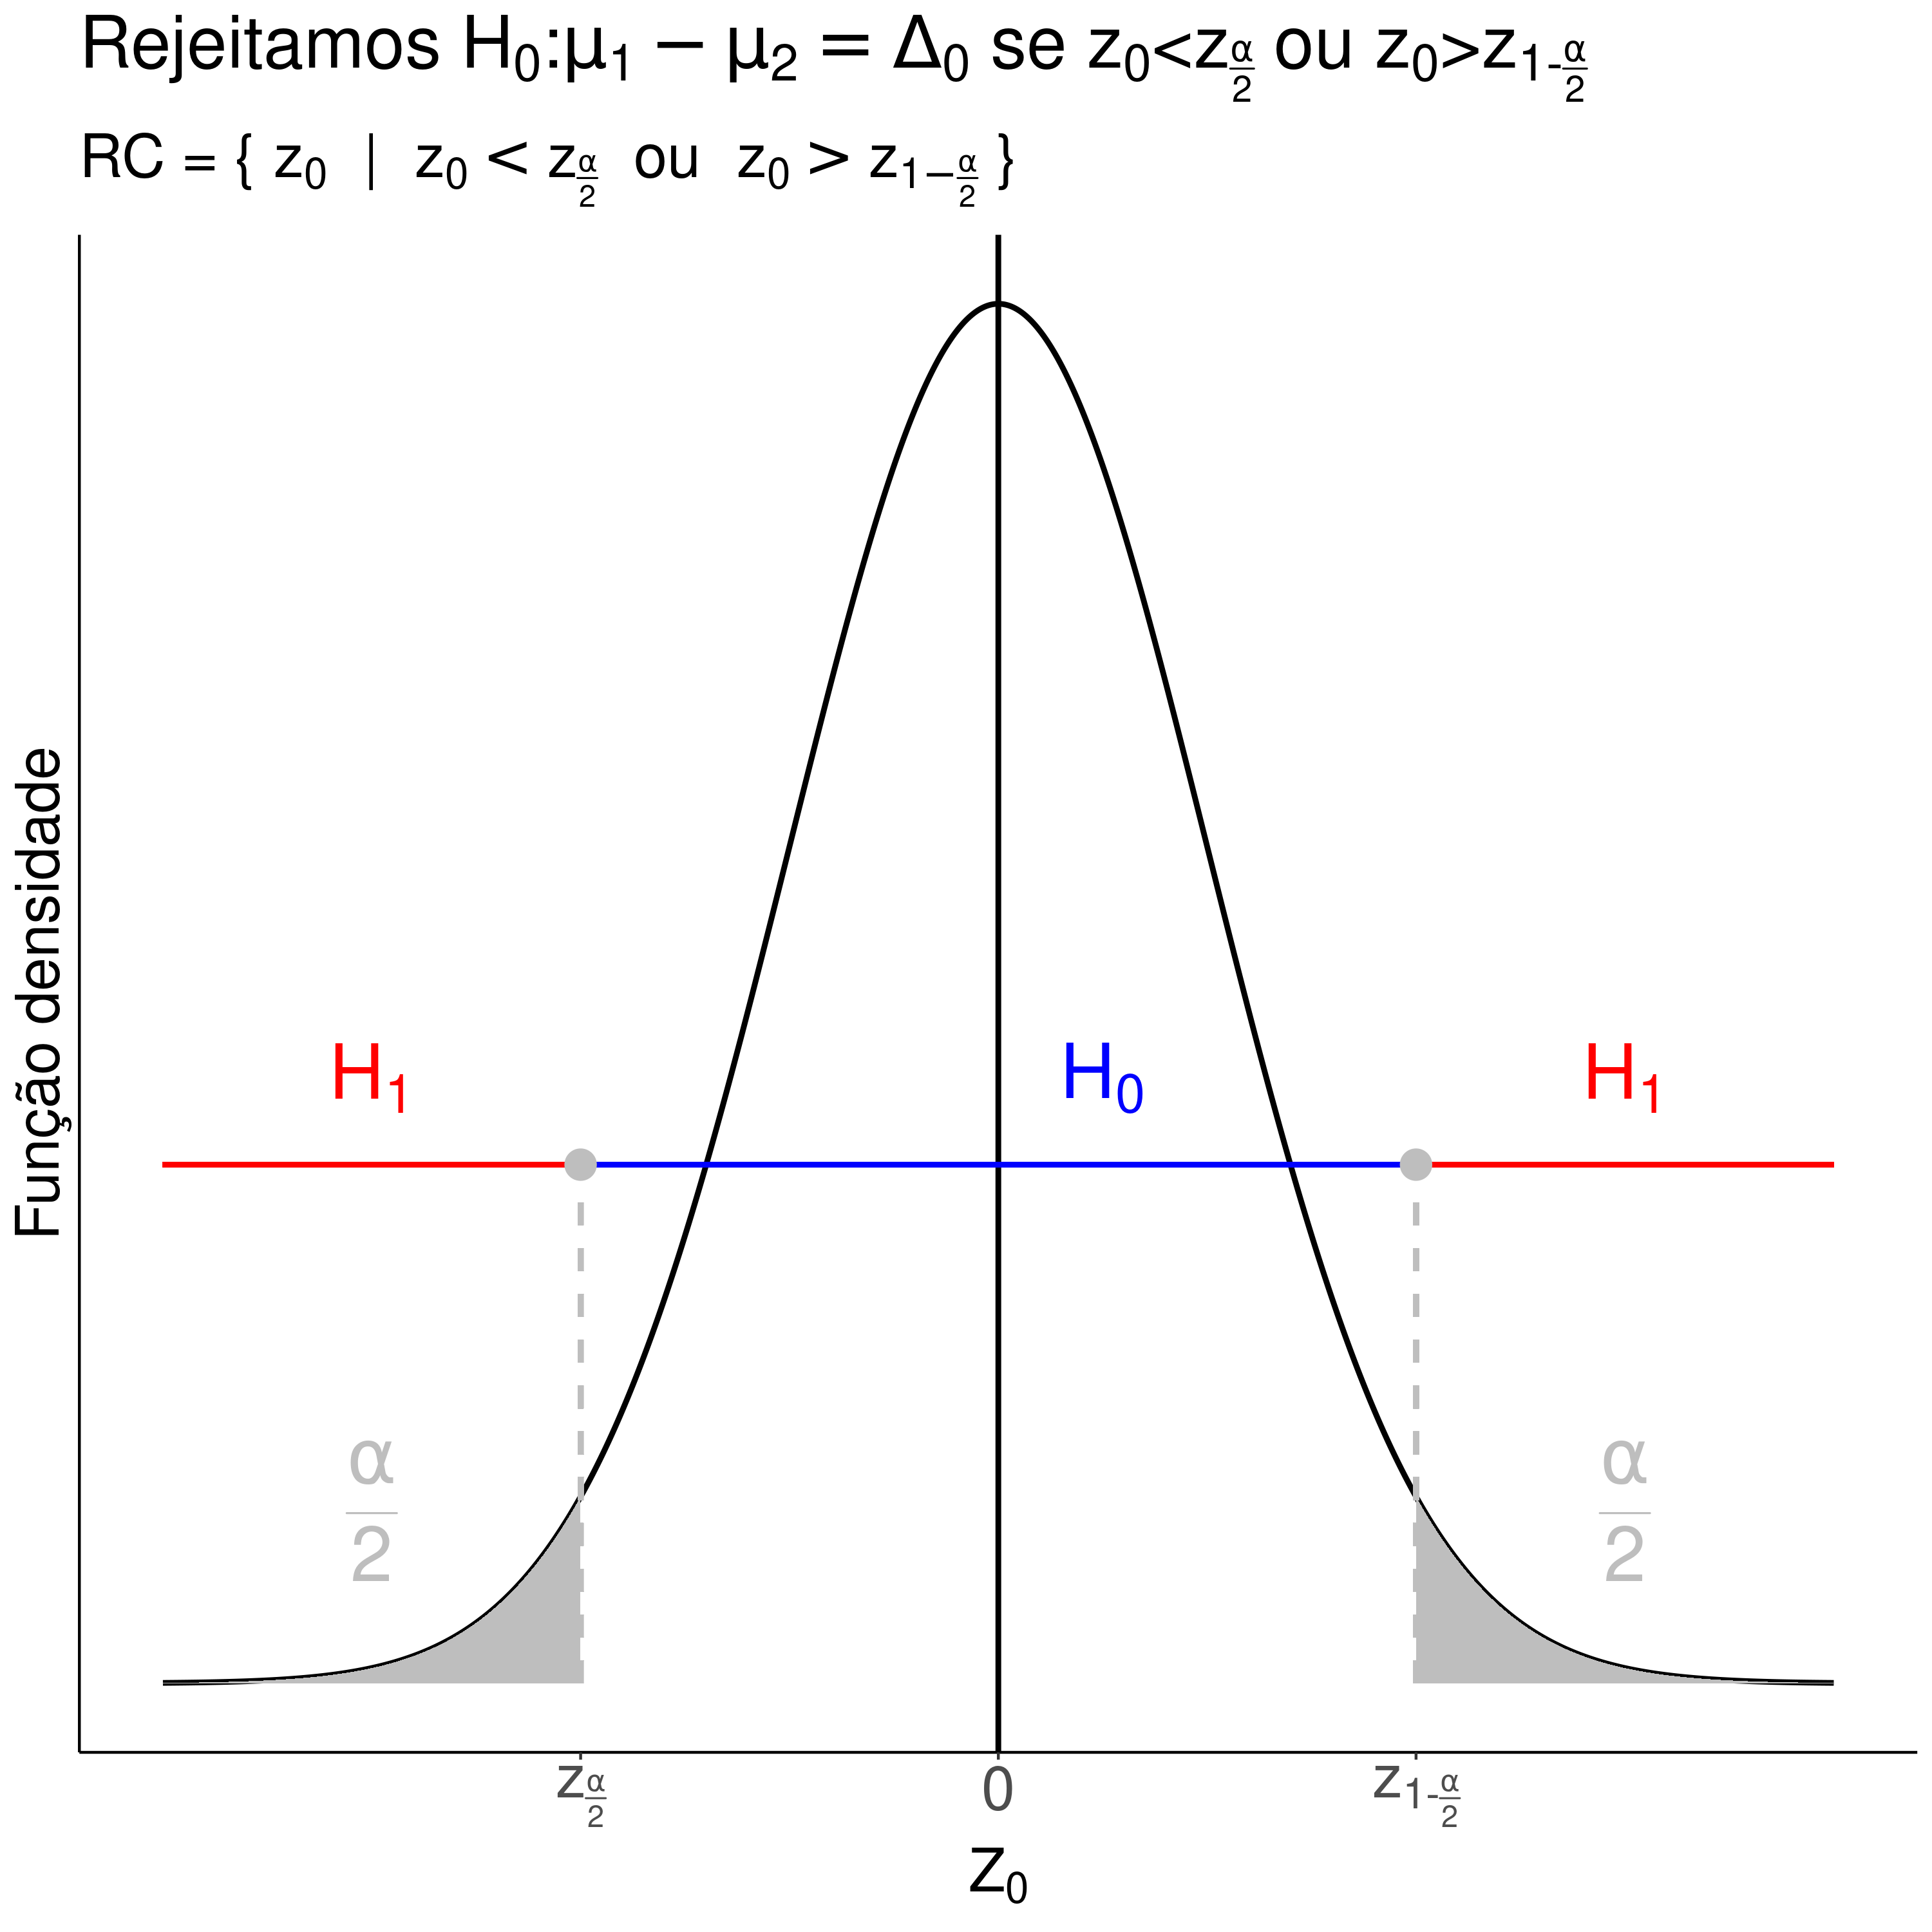
\includegraphics[width=0.32\linewidth]{figures/2-pop-normal-s2-known-bilateral.png} \label{fig:2-pop-normal-s2-known-bilateral}} \hfill
	\subfloat[][Teste bilateral.]{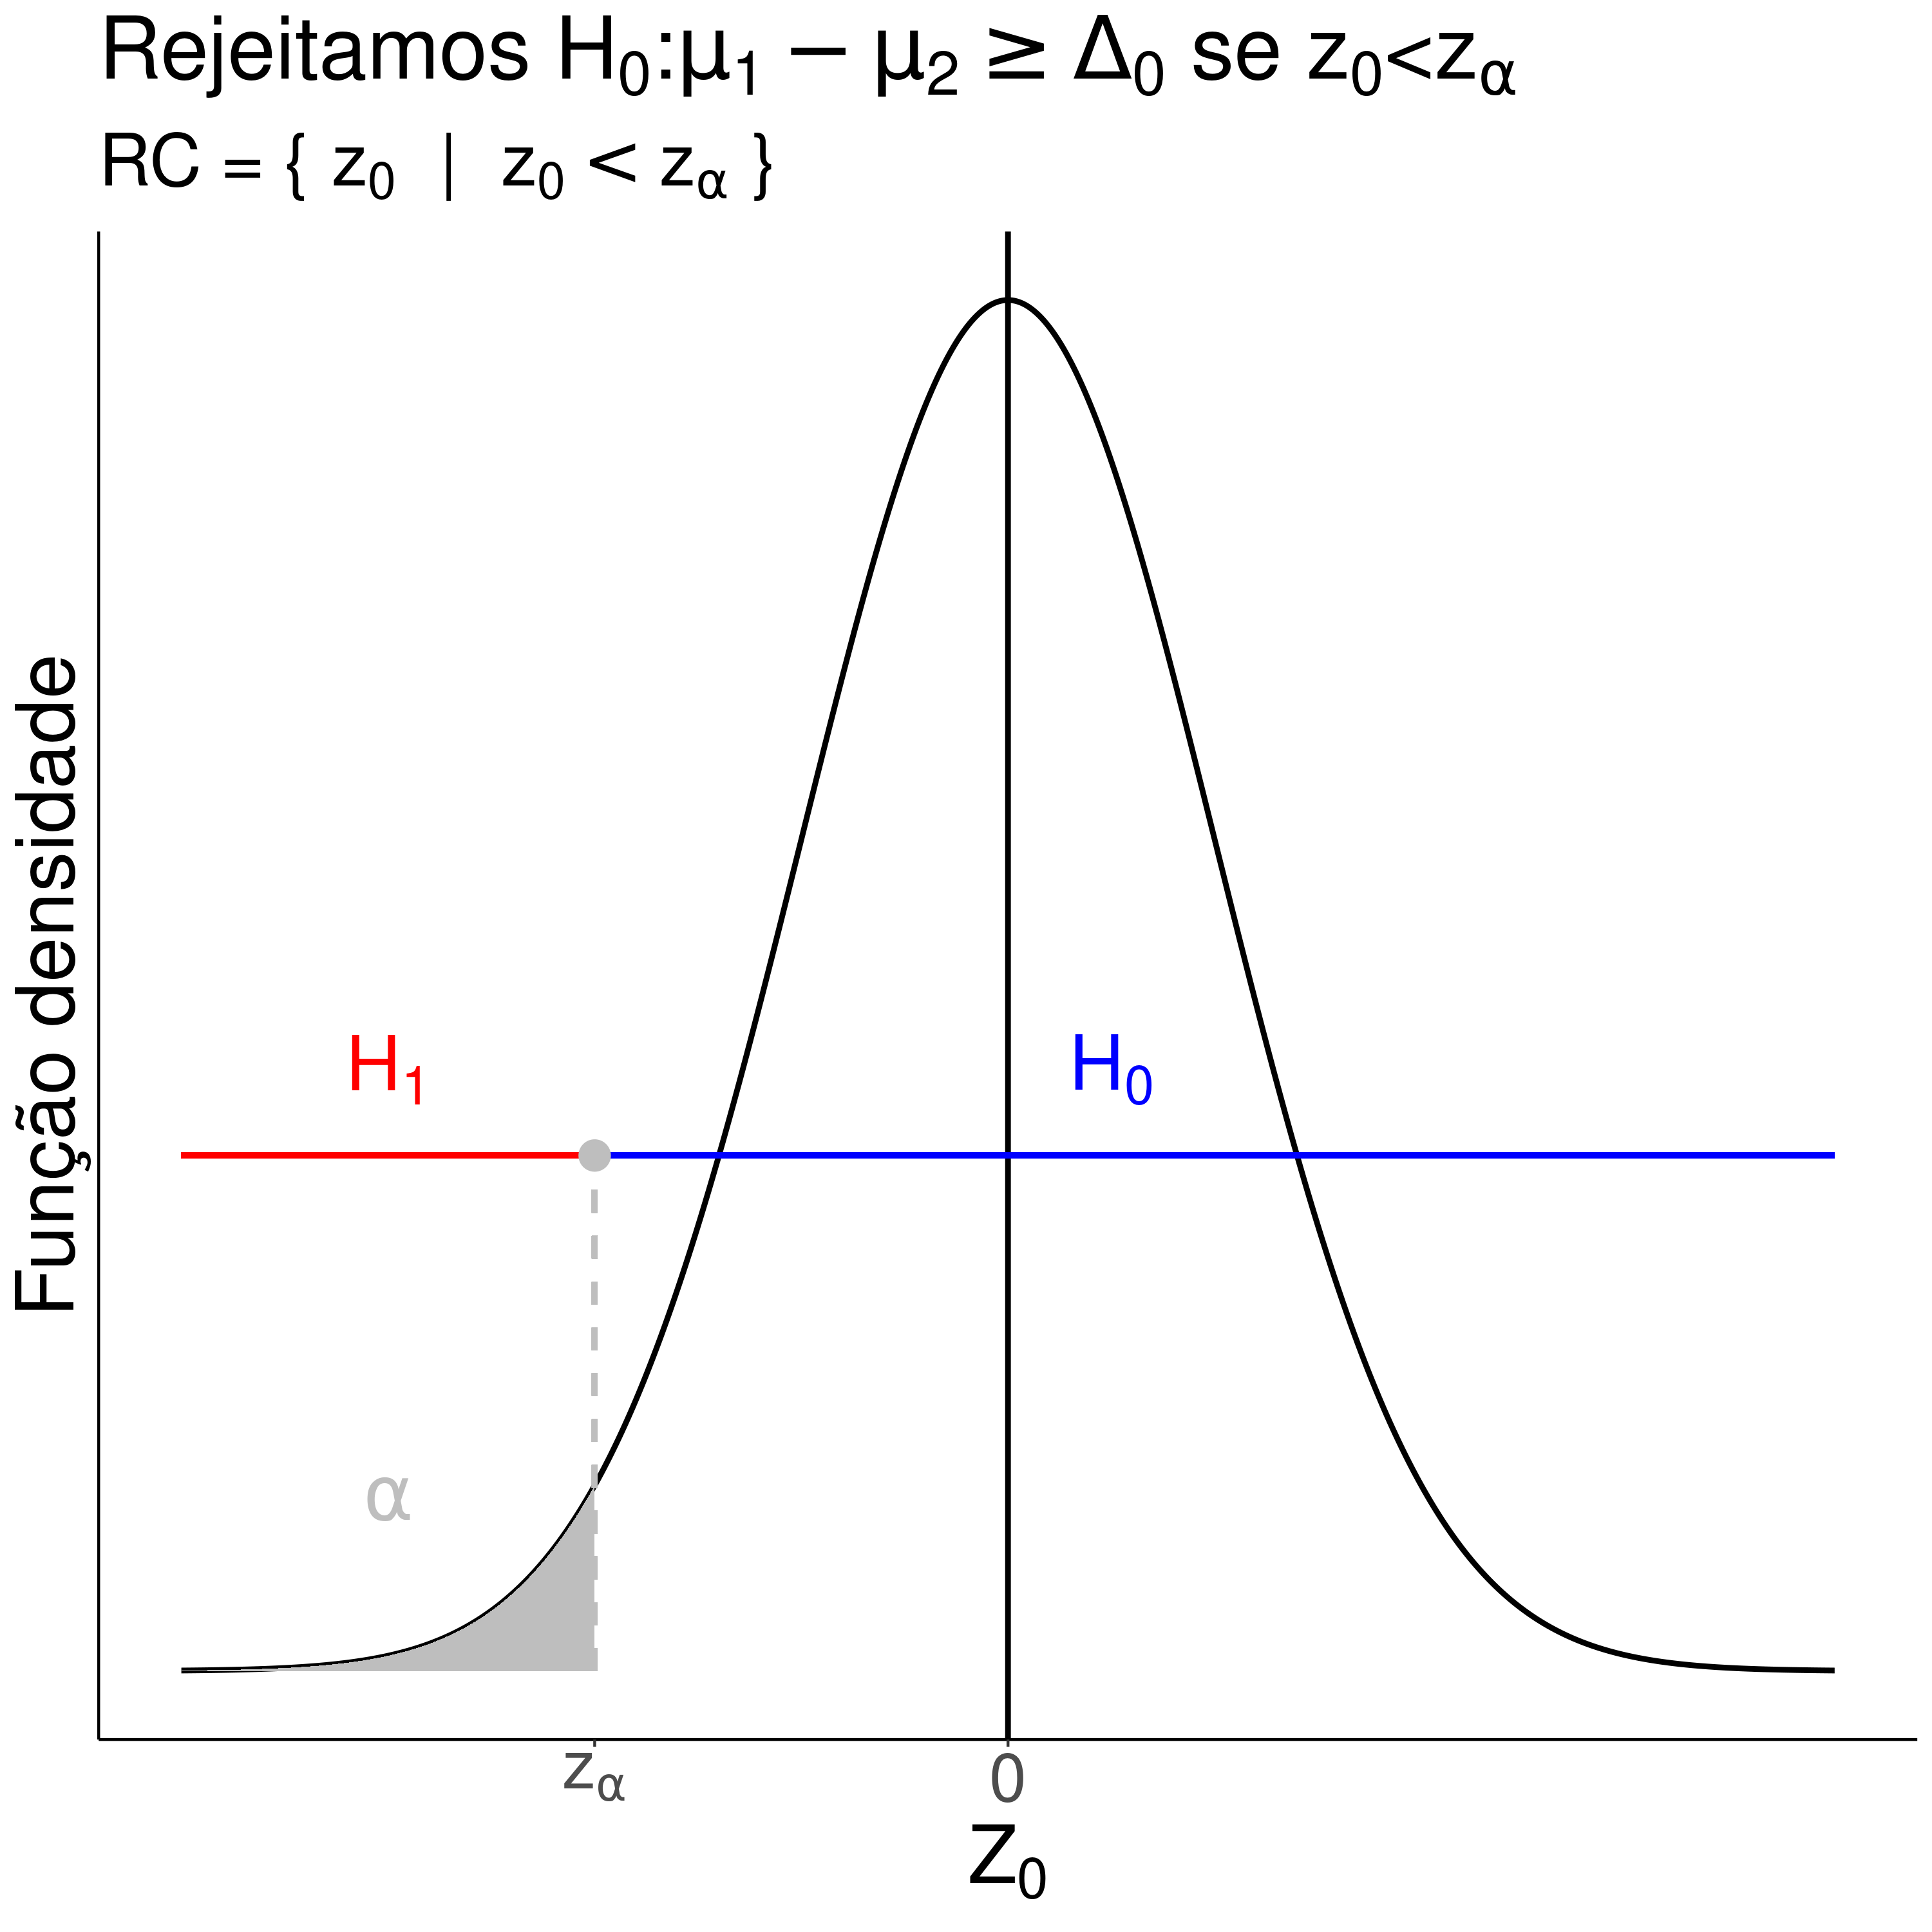
\includegraphics[width=0.32\linewidth]{figures/2-pop-normal-s2-known-h1-lower.png} \label{fig:2-pop-normal-s2-known-h1-lower}} \hfill
	\subfloat[][Teste bilateral.]{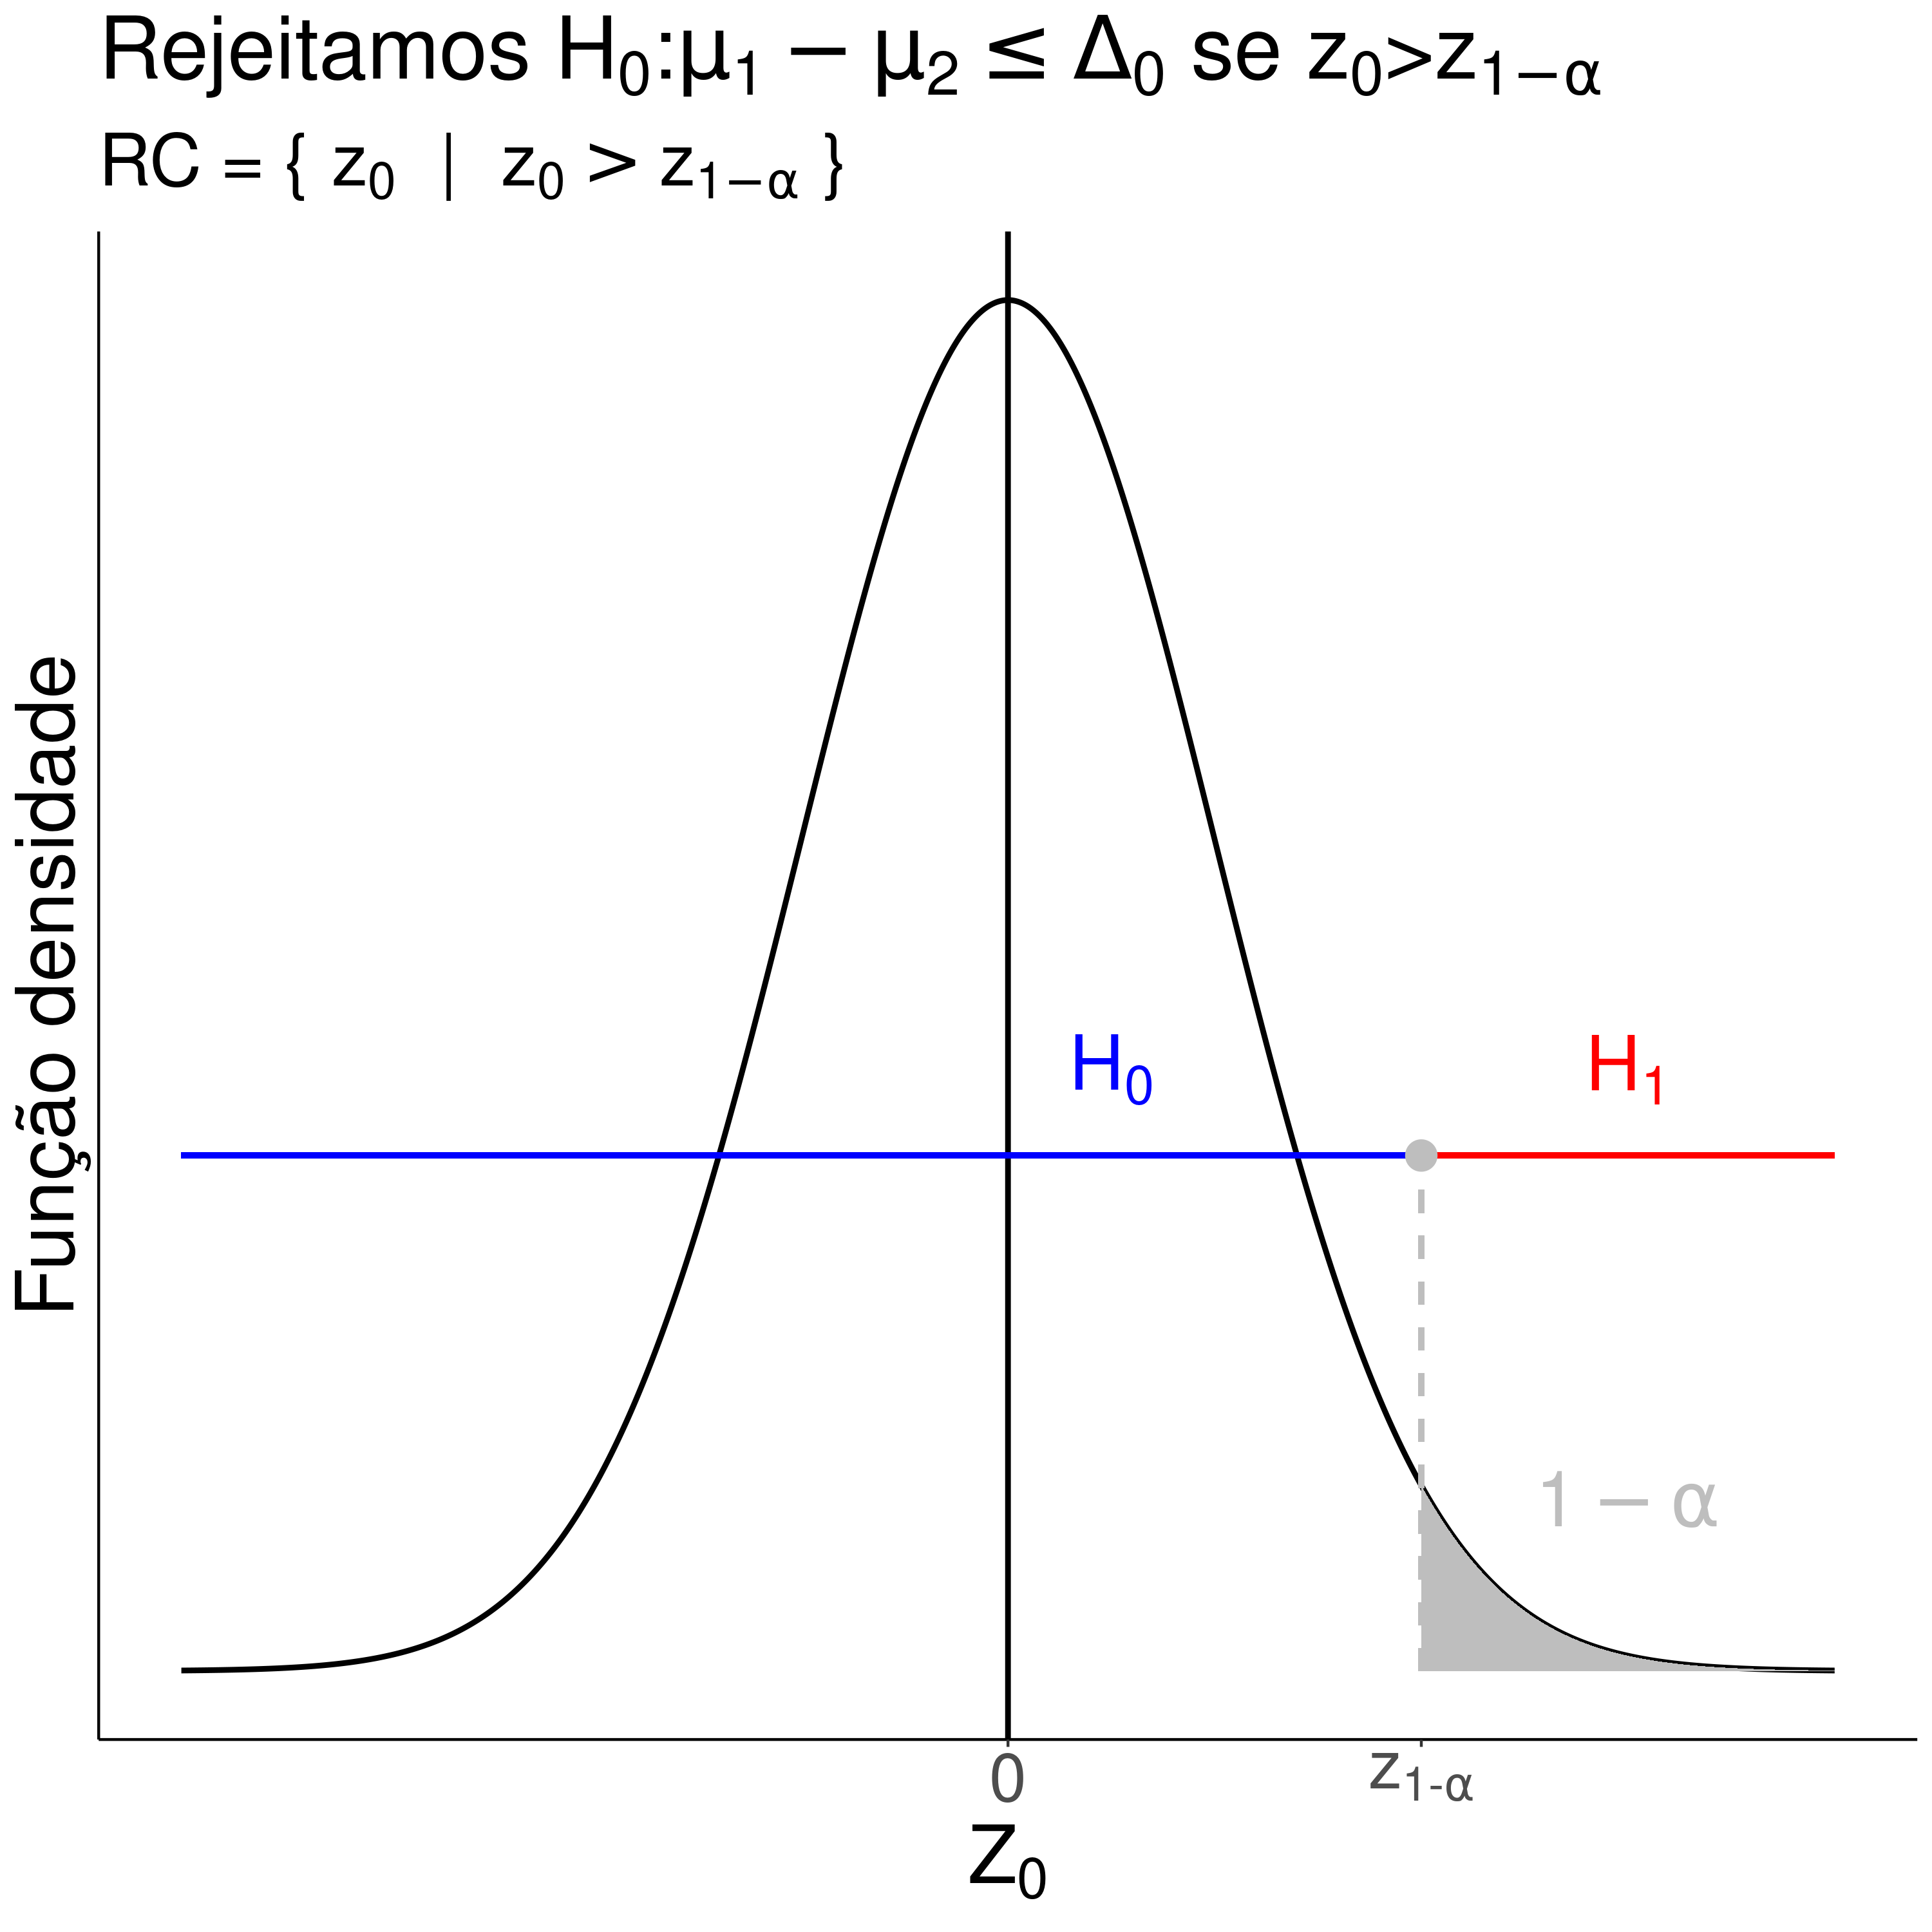
\includegraphics[width=0.32\linewidth]{figures/2-pop-normal-s2-known-h1-upper.png} \label{fig:2-pop-normal-s2-known-h1-upper}} 
	\caption{Região crítica para comparar médias de populações normais com variâncias conhecidas.}
\end{figure}
\end{frame}

\begin{frame}{Comparação de médias $\mu_1$ e $\mu_2$ de duas populações}

\begin{itemize}
	\item Na Figura~\ref{fig:2-pop-normal-s2-known-bilateral}, testamos $H_0: \mu_1 - \mu_2 = \Delta_0$ versus $H_1: \mu_1 - \mu_2 \neq 0$. Rejeitamos $H_0$ se $z_0 = \frac{\bar{x}_1 - \bar{x}_1 - \Delta_0}{ \sqrt{ \frac{\sigma_1^2}{n_1} + \frac{\sigma_2^2}{n_2} } } \in \allowbreak RC=\{z_0 \mid z_0 < z_\frac{\alpha}{2} \mbox{ ou } z_0 > z_{1-\frac{\alpha}{2}} \}$, em que $\Phi\left( z_\frac{\alpha}{2} \right) = \frac{\alpha}{2}$ e $\Phi\left( z_{1-\frac{\alpha}{2}} \right) = 1- \frac{\alpha}{2}$;
	\vfill
	
	\item Na Figura~\ref{fig:2-pop-normal-s2-known-h1-lower}, testamos $H_0: \mu_1 - \mu_2 \leq \Delta_0 $ versus $H_1: \mu_1 - \mu_2 > 0$. Rejeitamos $H_0$ se $z_0 = \frac{\bar{x}_1-\bar{x}_1  - \Delta_0}{\sqrt{ \frac{\sigma_1^2}{n_1} + \frac{\sigma_2^2}{n_2} }} \in \allowbreak RC=\{z_0 \mid z_0 > z_{1-\alpha}  \}$, em que $\Phi\left( z_{1-\alpha} \right) =1- \alpha$;
	\vfill
	
	\item Na Figura~\ref{fig:2-pop-normal-s2-known-h1-upper}, testamos $H_0: \mu_1 - \mu_2 \geq \Delta_0$ versus $H_1: \mu_1 - \mu_2  < 0$. Rejeitamos $H_0$ se $z_0 = \frac{\bar{x}_1-\bar{x}_1  - \Delta_0}{\sqrt{ \frac{\sigma_1^2}{n_1} + \frac{\sigma_2^2}{n_2} }} \in \allowbreak RC=\{z_0 \mid z_0 < z_{\alpha}  \}$, em que $\Phi\left( z_{\alpha} \right) = \alpha$.
\end{itemize}
Chamamos $z_\alpha$, $z_{1-\alpha}$, $z_\frac{\alpha}{2}$ e $z_{1-\frac{\alpha}{2}}$ são chamados de valores críticos.

\end{frame}

\begin{frame}{Comparação de médias $\mu_1$ e $\mu_2$ de duas populações}

\begin{block}{Exemplo}
	Duas máquinas em uma linha de produção preenchem garrafas \textit{pet} com $600ml$. Das especificações fornecidas pelos fabricantes das máquinas, sabe-se que o volume das garrafas tem distribuição normal e as máquinas são preenchidas com desvio padrão $\sigma_1=5cm^3$ e $\sigma_2=10cm^3$. Um membro da equipe de controle de qualidade, suspeita que o volume médio de preenchimento das garrafas são diferentes. Para isso, ele coletou 10 garrafas preenchidas pela máquina 1 e 10 garrafas da máquina 2. Os dados estão na Tabela~\ref{tab:volume-maquinas}. Ao nível de significância $\alpha=5\%$, as duas máquinas preenchem, em média, com volume diferente as garrafas?
	\begin{table}[ht]
		\centering
		\scalebox{0.65}{
		\begin{tabular}{l|cccccccccc}
			\toprule[0.05cm]
			amostra da máquina 1 & 599,67 & 600,74 & 599,49 & 600,56 & 599,65 & 599,72 & 600,34 & 600,17 & 599,87 & 599,44 \\ \midrule[0.025cm]
			amostra da máquina 2 & 600,18 & 599,66 & 600,36 & 601,47 & 600,57 & 602,25 & 601,19 & 601,07 & 600,81 & 599,26 \\ 
			\bottomrule[0.05cm]
		\end{tabular}
		}
		\caption{Amostras para as máquinas 1 e 2.} 
		\label{tab:volume-maquinas}
	\end{table}
\end{block}

\end{frame}

\begin{frame}{Comparação de médias $\mu_1$ e $\mu_2$ de duas populações}

\small
\begin{block}{Solução}
	\textbf{Passo 1)} Queremos testar as seguintes hipóteses: $H_0: \mu_1 - \mu_2 = \Delta_0 =0$ e $H_1: \mu_1 - \mu_2 \neq \Delta_0 = 0$;
	
	\textbf{Passo 2)} Nível de significância $\alpha=5\%$;
	
	\textbf{Passo 3)} Rejeitamos $H_0: \mu_1 - \mu_2 =0$ se $\lvert z_0 \rvert = \left\lvert \frac{\bar{x}_1 - \bar{x}_2 - \Delta_0}{\sqrt{ \frac{\sigma_1^2}{n_1} + \frac{\sigma_2^2}{n_2} }} \right\rvert$ for grande. Ou seja, $RC=\left\{ 
	 z_0 \mid z_0 < z_\frac{\alpha}{2} \mbox{ ou } z_{1-\frac{\alpha}{2}} < z_0  \right\}$;
	 
	\textbf{Passo 4)} Vamos encontrar os valores críticos:
	\begin{itemize}
		\item $\Phi\left( z_\frac{\alpha}{2} \right) = \Phi\left( z_{0,025} \right) = \frac{\alpha}{2} = 0,025$, então $z_{0,025} = -1,96$;
		\item $\Phi\left( z_{1-\frac{\alpha}{2}} \right) = \Phi\left( z_{0,975} \right) = 1 - \frac{\alpha}{2} = 0,975$, então $z_{0,975} = 1,96$.
	\end{itemize}
	 
	 \textbf{Passo 5)} Como $n_1=10$, $n_2=10$, $\sigma_1=5cm^3$, $\sigma_2=10cm^3$, $\bar{x}_1=599,965$, $\bar{x}_2=600,682 $, $\Delta_0 =0$ e $z_0=\frac{\bar{x}_1 - \bar{x}_2 - \Delta_0}{\sqrt{ \frac{\sigma_1^2}{n_1} + \frac{\sigma_2^2}{n_2} }}=-0,20$, então $z_0 \not\in RC$ e não rejeitamos $H_0$.
	 
	 Ou seja, ao nível de significância $\alpha=5\%$, não temos evidência para afirmar que as médias de volume das garrafas preenchidas pelas duas máquinas são diferentes.
\end{block}
\normalsize

\end{frame}

\begin{frame}{Comparação de médias $\mu_1$ e $\mu_2$ de duas populações}

\begin{block}{Solução (valor-p)}
	O valor-p é dado por
	$$p = P\left(\lvert Z \rvert > \lvert z_0 \rvert \mid H_0  \right) = 2 \left[ 1 - \Phi\left(\lvert z_0 \rvert\right) \right],$$
	em que $z_0 = \frac{\bar{x}_1 - \bar{x_2} - \Delta_0}{\sqrt{ \frac{\sigma_1^2}{n_1} + \frac{\sigma_2^2}{n_2} }}$.
	
	 Como $n_1=10$, $n_2=10$, $\sigma_1=0,6cm^3$, $\sigma_2=0,75cm^3$, $\bar{x}_1=599,965$, $\bar{x}_2=600,682 $ e $z_0=-0,20$, o valor-p é computador por
	 \begin{align*}
		 p &= 2 \left[1 -  \Phi\left(\lvert z_0 \rvert \right)\right]\\
		 &= 2 \left[ 1 - \Phi\left(\lvert -0,20 \rvert \right) \right]\\
		 &= 2 \left[ 1 - 0,5793 \right]\\
		 &= 0,8414.
	 \end{align*}
	 
	 Como $p=0,8414 \geq \alpha = 0,05$, não rejeitamos $H_0$ ao nível de significância $\alpha=5\%$. Ou seja, ao nível de significância $\alpha=5\%$, não temos evidência para afirmar que as duas máquinas preenchem as garrafas com volumes diferentes.
\end{block}

\end{frame}

\begin{frame}{Comparação de médias $\mu_1$ e $\mu_2$ de duas populações}

\begin{block}{Exemplo}
	Uma indústria química está interessada em reduzir o tempo de secagem de uma tinta usada em impressoras de pequeno porte. Duas fórmulas estão em teste: a formulação 1 é o padrão estabelecido na indústria, e a formulação 2 tem potencialmente um tempo de secagem da tinta menor. Da experiência e de informações do órgão regulador, os pesquisadores sabem que a formulação 1 tem tempo de secagem com desvio padrão de 8 segundo, e de uma amostra piloto os pesquisadores sabem que a fórmula 2 tem o desvio padrão de 9 segundos. Dez folhas são impressas com a fórmula 1 e vinte folhas são impressas com a fórmula 2. O tempo médio de secagem na amostra com a fórmula 1 é $\bar{x}_1 = 49,53$ segundos e o tempo médio de secagem na amostra com a fórmula 2 (menos custosa) é $\bar{x}_2 = 39,42$ segundos. Ao nível de significância $\alpha=5\%$, a tinta da fórmula 2 seca mais rápido?
\end{block}

\end{frame}

\begin{frame}{Comparação de médias $\mu_1$ e $\mu_2$ de duas populações}

\small

\begin{block}{Solução}
	\textbf{Passo 1)} Temos as seguintes hipóteses: $H_0: \mu_1 - \mu_2 \leq \Delta_0 = 0$ e $H_1: \mu_1 - \mu_2 > \Delta_0 = 0$;
	
	\textbf{Passo 2)} Nível de significância $\alpha = 5\%$;
	
	\textbf{Passo 3)} Rejeitamos $H_0: \mu_1 - \mu_2 = 0$ se $ z_0 =  \frac{\bar{x}_1 - \bar{x}_2 - \Delta_0}{\sqrt{ \frac{\sigma_1^2}{n_1} + \frac{\sigma_2^2}{n_2} }} $ for pequeno. Ou seja, $RC = \left\{ z_0 \mid z_0 > z_{1-\alpha}	 \right\}$;
	 
	 \textbf{Passo 4)} Vamos encontrar os valores críticos:
	 \begin{itemize}
	 	\item $\Phi\left( z_{1-\alpha} \right) = \Phi\left( z_{0,95} \right) = 1-\alpha = 0,95$, então $z_{0,95} = 1,65$.
	 \end{itemize}
 
 	\textbf{Passo 5)} Como $n_1=10$, $n_2=20$, $\sigma_1=8$, $\sigma_2 = 9$, $\bar{x}_2=49,53$, $\bar{x}_1 = 39,42$ e $ z_0  =  \frac{ \bar{x}_1 - \bar{x}_2  -\Delta_0}{ \sqrt{ \frac{\sigma_1^2}{n_1} + \frac{\sigma_2^2}{n_2} } }  = \frac{ 49,53-39,42  }{ \sqrt{ \frac{8^2}{10} + \frac{9^2}{20} }  }  = 3,13$, então $3,13 \in RC$ e rejeitamos $H_0$. Ou seja, ao nível de significância $\alpha=5\%$, rejeitamos $H_0$ e o tempo médio de secagem da tinta da fórmula 2 é menor. 
\end{block}

\normalsize

\end{frame}

\begin{frame}{Comparação de médias $\mu_1$ e $\mu_2$ de duas populações}

\begin{block}{Solução (valor-p)}
	O valor-p é calculado através de
	$$p = P \left(  Z  >  z_0  \mid H_0 \right) =  1 - \Phi \left(z_0\right),$$
	em que $Z \sim N(0,1)$.
	
	Como $n_1=10$, $n_2=20$, $\sigma_1=8$, $\sigma_2 = 9$, $\bar{x}_2=49,53$, $\bar{x}_1 = 39,42$ e $ z_0  = \frac{ \bar{x}_1 - \bar{x}_2 -\Delta_0 }{ \sqrt{ \frac{\sigma_1^2}{n_1} + \frac{\sigma_2^2}{n_2} } }  =  \frac{ 49,53-39,42   }{ \sqrt{ \frac{8^2}{10} + \frac{9^2}{20} }  }  = 3,13$, o valor-p -e calculado através de
	\begin{align*}
		p &= 1 - \Phi \left(z_0\right) \\
		&=  1 - \Phi(3,13) \\
		&=1 - 0,9991\\
		&=0,0009.
	\end{align*}
	
	Como $p=0,0009 < \alpha = 0,05$, rejeitamos $H_0$ ao nível de significância $\alpha=5\%$, ou seja, a tinta com a fórmula 2 seca mais rápido ao nível de significância $5\%$.
\end{block}

\end{frame}

\begin{frame}{Comparação de médias $\mu_1$ e $\mu_2$ de duas populações}

\begin{block}{Exemplo}
	
\end{block}
Imagine que temos duas populações com distribuições normais com variâncias populacionais e que um pesquisador precisa decidir entre as duas hipóteses $H_0: \mu_1 - \mu_2 \geq 0$ e $H_1: \mu_1 - \mu_2 < 0$. Na Tabela~\ref{tab:comparacao-medias} colocamos algumas informações sobre o experimento. Complete a Tabela~\ref{tab:comparacao-medias}. Qual a sua decisão?  Calcule o valor-p.
\begin{table}[htbp]
	\centering
		\begin{tabular}{c|c|c|c|c}
			\toprule[0.05cm]
			$z_0$ & Decisão & valor-p & $\bar{x}_1$ &$\bar{x}_2$\\ \midrule[0.025cm]
			& & & $14,2$ & $19,7$ \\ 
			\midrule[0.05cm]
			$n_1$ & $n_2$ & $\sigma_1$ & $\sigma_2$ & Nível de significância $\alpha$\\ \midrule[0.025cm]
			$10$ & $15$ & $10$ & $5$ & $5\%$\\ \bottomrule[0.05cm]
		\end{tabular}
	\caption{Algumas informações sobre o experimento.}
	\label{tab:comparacao-medias}
\end{table}
\end{frame}

\begin{frame}{Comparação de médias $\mu_1$ e $\mu_2$ de duas populações}

\begin{block}{Solução}
	\textbf{Passo 1)} Queremos testar as hipóteses: $H_0: \mu_1 - \mu_2 \geq \Delta_0 = 0$  e $H_1: \mu_1 - \mu_2 < \Delta_0 = 0$;
	
	\textbf{Passo 2)} Nível de significância: $\alpha=5\%$;
	
	\textbf{Passo 3)} Rejeitamos $H_0$ se $z_0 = \frac{\bar{x}_1 - \bar{x}_2 - \Delta_0}{\sqrt{ \frac{\sigma_1^2}{n_1} + \frac{\sigma_2^2}{n_2} }}$ for pequeno. Ou seja, $RC=\left\{ z_0 \mid z_0 < z_\alpha \right\}$;
	
	\textbf{Passo 4)} Vamos encontrar o valor crítico:
	\begin{itemize}
		\item $\Phi\left( z_\alpha \right) = \Phi\left( z_{0,05} \right) = \alpha = 0,05$, então $z_{0,05} = -1,65$;
	\end{itemize}

	\textbf{Passo 5)} Primeiro calculamos a estatística do teste usando as informações da Tabela~\ref{tab:comparacao-medias}:
	\begin{align*}
		z_0 &= \frac{\bar{x}_1 - \bar{x}_2 - \Delta_0}{\sqrt{ \frac{\sigma_1^2}{n_1} + \frac{\sigma_2^2}{n_2} }} = \frac{ 14,2 - 19,7 }{ \sqrt{ \frac{10^2}{10} + \frac{5^2}{15} } } = -1,61,
	\end{align*}
	Como $z_0 \not\in RC$ e não rejeitamos $H_0$ ao  nível de significância $\alpha=5\%$.
\end{block}

\end{frame}

\begin{frame}{Comparação de médias $\mu_1$ e $\mu_2$ de duas populações}
\begin{block}{Solução (valor-p)}
	Calculamos o valor através de 
	$$p=P\left( Z_0 < z_0 \mid H_0 \right) = \Phi\left( z_0 \right).$$
	
	Usando as informações da Tabela~\ref{tab:comparacao-medias}, temos que $z_0 = \frac{\bar{x}_1 - \bar{x}_2 - \Delta_0}{\sqrt{ \frac{\sigma_1^2}{n_1} + \frac{\sigma_2^2}{n_2} }} = \frac{ 14,2 - 19,7 }{ \sqrt{ \frac{10^2}{10} + \frac{5^2}{15} } } = -1,61$ e o valor-p é dado por:
	$$p = \Phi \left( z_0 \right) =  \Phi\left(-1,61\right) = 0,0537.$$
	
	Como $p=0,0537 > \alpha = 0,05$, não rejeitamos $H_0$ ao nível de significância $\alpha=5\%$.
\end{block}
\end{frame}

\begin{frame}{Poder do teste: $H_0:\mu_1 - \mu_2 = \Delta_0$ e $H_1: \mu_1 - \mu_2 \neq \Delta_0$.}

\tiny

Imagine que
\begin{itemize}
	\item Hipóteses: $H_0: \mu_1 - \mu_2 = \Delta_0$ e $H_1: \mu_1 -  \mu_2 \neq \Delta_0$;
	\item $H_1$ é verdade, então $\Delta = \mu_1-\mu_2 \neq \Delta_0$;
	\item $Z_0 = \frac{\bar{X}_1 - \bar{X}_2 - \Delta_0}{ \sqrt{ \frac{\sigma_1^2}{n_1} + \frac{\sigma_2^2}{n_2} } } \sim N\left( \frac{\Delta - \Delta_0}{ \sqrt{ \frac{\sigma_1^2}{n_1} + \frac{\sigma_2^2}{n_2} } } ; 1\right)$;
	\item Ao nível de significância $\alpha$, temos $RC = \{ z_0 \mid z_0 < z_{\frac{\alpha}{2}} \mbox{ ou } z_{1-\frac{\alpha}{2}} < z_0  \}$.
\end{itemize}
\vfill	

Poder do teste é dado
\begin{align*}
\textcolor{important}{1-\beta} &=1 - \left[P\left( z_\frac{\alpha}{2} \leq Z_0 \leq z_{1 - \frac{\alpha}{2}} \mid H_1 \right)\right]\\
& = 1- \left[ P \left( z_\frac{\alpha}{2} - \frac{\Delta - \Delta_0}{ \sqrt{ \frac{\sigma_1^2}{n_1} + \frac{\sigma_2^2}{n_2} } } \leq Z_0 - \frac{\Delta - \Delta_0}{ \sqrt{ \frac{\sigma_1^2}{n_1} + \frac{\sigma_2^2}{n_2} } } \leq z_{1 - \frac{\alpha}{2}} - \frac{\Delta - \Delta_0}{ \sqrt{ \frac{\sigma_1^2}{n_1} + \frac{\sigma_2^2}{n_2} } } \mid \Delta \neq \Delta_0 \right)\right]\\
&= \textcolor{important}{1 - \Phi\left( z_{1-\frac{\alpha}{2}} - \frac{\Delta - \Delta_0}{ \sqrt{ \frac{\sigma_1^2}{n_1} + \frac{\sigma_2^2}{n_2} } } \right) + \Phi\left( z_{\frac{\alpha}{2}} - \frac{\Delta - \Delta_0}{ \sqrt{ \frac{\sigma_1^2}{n_1} + \frac{\sigma_2^2}{n_2} } } \right).}
\end{align*}
\vfill

A \textcolor{important}{Função Poder}, dado o tamanho da amostra $n$, é uma função das médias populacionais na hipótese alternativa  $\pi: \mathbb{R} - \{\Delta_0\} \longrightarrow [0,1]$ dada por
\begin{align*}
\pi(\delta) = 1 - \Phi\left( z_{1-\frac{\alpha}{2}} - \frac{\Delta - \Delta_0}{ \sqrt{ \frac{\sigma_1^2}{n_1} + \frac{\sigma_2^2}{n_2} } } \right) + \Phi\left( z_{\frac{\alpha}{2}} - \frac{\Delta - \Delta_0}{ \sqrt{ \frac{\sigma_1^2}{n_1} + \frac{\sigma_2^2}{n_2} } } \right), \qquad \Delta = \mu_1 - \mu_2, \Delta \in \mathbb{R} - \{\Delta_0 \}.
\end{align*}
Alguns livros chamada a Função Poder de \textcolor{important}{Curva de Característica Operacional.}

\normalsize

\end{frame}

\subsection{Poder e tamanho da amostra.}

\begin{frame}{Tamanho da amostra: $H_0:\mu_1 - \mu_2 = \Delta_0$ e $H_1: \mu_1 - \mu_2 \neq \Delta_0$.}

\footnotesize

Imagine que
\begin{itemize}
	\item Hipóteses: $H_0: \mu_1 - \mu_2 = \Delta_0$ e $H_1: \mu_1 -  \mu_2 \neq \Delta_0$;
	\item $H_1$ é verdade, então $\Delta = \mu_1-\mu_2 \neq \Delta_0$;
	\item $Z_0 = \frac{\bar{X}_1 - \bar{X}_2 - \Delta_0}{ \sqrt{ \frac{\sigma_1^2}{n_1} + \frac{\sigma_2^2}{n_2} } } \sim N\left( \frac{\Delta - \Delta_0}{ \sqrt{ \frac{\sigma_1^2}{n_1} + \frac{\sigma_2^2}{n_2} } } ; 1\right)$;
	\item Ao nível de significância $\alpha$, temos $RC = \{ z_0 \mid z_0 < z_{\frac{\alpha}{2}} \mbox{ ou } z_{1-\frac{\alpha}{2}} < z_0  \}$.
\end{itemize}
\vfill

Assuma as seguintes simplificações:
\begin{itemize}
	\item Se $\Delta > \Delta_0$, então $\Phi\left( z_\frac{\alpha}{2} - \frac{\Delta - \Delta_0}{ \sqrt{ \frac{\sigma_1^2}{n_1} + \frac{\sigma_2^2}{n_2} } } \right) \approx 0$;
	\item Se $\Delta < \Delta_0$, então $\Phi\left( z_{1-\frac{\alpha}{2}} - \frac{\Delta - \Delta_0}{ \sqrt{ \frac{\sigma_1^2}{n_1} + \frac{\sigma_2^2}{n_2} } } \right) \approx 1$.
\end{itemize}

Então, o tamanho \sout{mínimo} da amostra é dado por
\begin{align*}
	n_1 = n_2 = n = \left\lceil \left( \frac{z_{1-\beta} + z_{1-\frac{\alpha}{2}}}{\Delta - \Delta_0} \right)^2 (\sigma_1^2 + \sigma_2^2) \right\rceil.
\end{align*}

\normalsize
\end{frame}

\begin{frame}{Poder do teste: $H_0:\mu_1 - \mu_2 = \Delta_0$ e $H_1: \mu_1 - \mu_2 \neq \Delta_0$.}

\begin{block}{Exemplo}
	Duas máquinas em uma linha de produção preenchem garrafas \textit{pet} com $600ml$. Das especificações fornecidas pelos fabricantes das máquinas, sabe-se que o volume das garrafas tem distribuição normal e as máquinas são preenchidas com desvio padrão $\sigma_1=5cm^3$ e $\sigma_2=10cm^3$. Um membro da equipe de controle de qualidade, suspeita que o volume médio de preenchimento das garrafas são diferentes. Para isso, ele coletou 10 garrafas preenchidas pela máquina 1 e 10 garrafas da máquina 2. Suponha que a máquina 1 enche as garrafas com média populacional $\mu_1=650ml$ e a máquina 2 enche as garrafas com média populacional $\mu_2=700ml$. Ao nível de significância $\alpha=5\%$, qual o poder do teste?	
\end{block}
\end{frame}

\begin{frame}{Poder do teste: $H_0:\mu_1 - \mu_2 = \Delta_0$ e $H_1: \mu_1 - \mu_2 \neq \Delta_0$.}

\footnotesize

\begin{block}{Solução}
	\textbf{Passo 1)} Queremos testar as hipóteses: $H_0: \mu_1 - \mu_2 = \Delta_0$ e $H_1= \mu_1 - \mu_2 \neq \Delta_0$;
	
	\textbf{Passo 2)} Nível de significância $\alpha=5\%$;
	
	Note que $\mu_1=650ml$, $\mu_2=700ml$, $\Delta=\mu_1-\mu_2=650-700=-50ml$, $\sigma_1=5cm^3$, $\sigma_2^2 = 10cm^3$, $n_1=n_2=10$.
	
	Primeiro encontramos os quantis da distribuição normal padrão:
	\begin{itemize}
		\item $\Phi\left(z_{\frac{\alpha}{2}}\right) = \Phi\left(z_{0,025}\right) = \frac{\alpha}{2} = 0,025$, então $z_{0,025} = -1,96$;
		\item  $\Phi\left(z_{1-\frac{\alpha}{2}}\right) = \Phi\left(z_{0,975}\right) =1- \frac{\alpha}{2} = 0,975$, então $z_{0,975} = 1,96$.
	\end{itemize}
	Então o o poder do teste é dado por:
	\begin{align*}
		1-\beta &= 1 - \Phi\left( z_{1-\frac{\alpha}{2}} - \frac{ \Delta - \Delta_0 }{ \sqrt{ \frac{\sigma_1^2}{n_1} + \frac{\sigma_2^2}{n_2} } } \right) + \Phi\left( z_{\frac{\alpha}{2}} - \frac{ \Delta - \Delta_0 }{ \sqrt{ \frac{\sigma_1^2}{n_1} + \frac{\sigma_2^2}{n_2} } } \right)\\ 
		&= 1- \Phi\left( 1,96 - \frac{-50}{\sqrt{ \frac{5^2}{10} + \frac{10^2}{10} }} \right) + \Phi\left( -1,96 - \frac{-50}{\sqrt{ \frac{5^2}{10} + \frac{10^2}{10} }} \right) = 1.
	\end{align*}
\end{block}

\normalsize
\end{frame}

\begin{frame}{Tamanho da amostra: $H_0:\mu_1 - \mu_2 = \Delta_0$ e $H_1: \mu_1 - \mu_2 \neq \Delta_0$.}

\begin{block}{Exemplo}
	Duas máquinas em uma linha de produção preenchem garrafas \textit{pet} com $600ml$. Das especificações fornecidas pelos fabricantes das máquinas, sabe-se que o volume das garrafas tem distribuição normal e as máquinas são preenchidas com desvio padrão $\sigma_1=5cm^3$ e $\sigma_2=10cm^3$. Um membro da equipe de controle de qualidade, suspeita que o volume médio de preenchimento das garrafas são diferentes. Suponha que a máquina 1 tem enche as garrafas com média populacional $\mu_1=690ml$ e a máquina 2 enche as garrafas com média populacional $\mu_2=700ml$. Ao nível de significância $\alpha=5\%$ e com poder do teste $1-\beta=99\%$, equipe de controle de qualidade precisa analisar quantas garrafas da máquina 1 e da máquina 2?	
\end{block}
\end{frame}

\begin{frame}{Tamanho da amostra: $H_0:\mu_1 - \mu_2 = \Delta_0$ e $H_1: \mu_1 - \mu_2 \neq \Delta_0$.}

\normalsize

\begin{block}{Solução}
	\textbf{Passo 1)} Queremos testar as hipóteses: $H_0: \mu_1 - \mu_2 = \Delta_0$ e $H_1= \mu_1 - \mu_2 \neq \Delta_0$;
	
	\textbf{Passo 2)} Nível de significância $\alpha=5\%$;
	
	Note que $\mu_1=690ml$, $\mu_2=700ml$, $\Delta=\mu_1-\mu_2=690-700=-10ml$, $\Delta_0=0$, $\sigma_1=5cm^3$, $\sigma_2 = 10cm^3$, $\alpha = 5\%$ e $1-\beta=95\%$. 
	
	Primeiro calculamos os quantis da distribuição normal padrão:
	\begin{itemize}
		\item $\Phi\left(z_{1-\beta}\right)=\Phi\left(z_{0,95}\right) = 1-\beta=0,95$, então $z_{0,95} = 1,65$;
		\item $\Phi\left(z_{1-\frac{\alpha}{2}}\right)=\Phi\left(z_{0,975}\right) = 1-\frac{\alpha}{2}=0,975$, então $z_{0,975} = 1,96$.
	\end{itemize}

	Então, o tamanho \sout{mínimo} da amostra de cada população é dado por
	\begin{align*}
	n_1=n_2&=n=\left\lceil \left( \frac{z_{1-\beta} + z_{1-\frac{\alpha}{2}}}{ \Delta - \Delta_0 } \right)^2 (\sigma_1^2 + \sigma_2^2) \right\rceil\\
	&= \left\lceil \left( \frac{1,65 + 1,96}{50} \right)^2 (5^2 + 10^2)  \right\rceil = 17.
	\end{align*}
\end{block}

\normalsize
\end{frame}


\begin{frame}{Poder do teste: $H_0:\mu_1 - \mu_2 \leq \Delta_0$ e $H_1: \mu_1 - \mu_2 > \Delta_0$.}

\tiny

Imagine que
\begin{itemize}
	\item Hipóteses: $H_0: \mu_1 - \mu_2 \leq \Delta_0$ e $H_1: \mu_1 -  \mu_2 > \Delta_0$;
	\item $H_1$ é verdade, então $\Delta = \mu_1-\mu_2 \neq \Delta_0$;
	\item $Z_0 = \frac{\bar{X}_1 - \bar{X}_2 - \Delta_0}{ \sqrt{ \frac{\sigma_1^2}{n_1} + \frac{\sigma_2^2}{n_2} } } \sim N\left( \frac{\Delta - \Delta_0}{ \sqrt{ \frac{\sigma_1^2}{n_1} + \frac{\sigma_2^2}{n_2} } } ; 1\right)$;
	\item Ao nível de significância $\alpha$, temos $RC = \{ z_0 \mid z_0 > z_{1-\alpha}  \}$.
\end{itemize}
\vfill	

Poder do teste é dado
\begin{align*}
\textcolor{important}{1-\beta} &=1 - \left[P\left( Z_0 \leq z_{1-\alpha} \mid H_1 \right)\right] = 1- \left[ P \left( Z_0 - \frac{\Delta - \Delta_0}{ \sqrt{ \frac{\sigma_1^2}{n_1} + \frac{\sigma_2^2}{n_2} } } \leq z_{1 - \alpha} - \frac{\Delta - \Delta_0}{ \sqrt{ \frac{\sigma_1^2}{n_1} + \frac{\sigma_2^2}{n_2} } } \mid \Delta \neq \Delta_0 \right)\right]\\
&= \textcolor{important}{1 - \Phi\left( z_{1-\alpha} - \frac{\Delta - \Delta_0}{ \sqrt{ \frac{\sigma_1^2}{n_1} + \frac{\sigma_2^2}{n_2} } } \right) }
\end{align*}
\vfill

A \textcolor{important}{Função Poder}, dado o tamanho da amostra $n$, é uma função das médias populacionais na hipótese alternativa  $\pi: (\Delta_0, \infty) \longrightarrow [0,1]$ dada por
\begin{align*}
\pi(\delta) = 1 - \Phi\left( z_{1-\alpha} - \frac{\Delta - \Delta_0}{ \sqrt{ \frac{\sigma_1^2}{n_1} + \frac{\sigma_2^2}{n_2} } } \right), \qquad \Delta = \mu_1 - \mu_2, \Delta \in (\Delta_0, \infty).
\end{align*}
Alguns livros chamada a Função Poder de \textcolor{important}{Curva de Característica Operacional.}

\normalsize

\end{frame}

\begin{frame}{Tamanho da amostra: $H_0:\mu_1 - \mu_2 \leq \Delta_0$ e $H_1: \mu_1 - \mu_2 > \Delta_0$.}

\large

Imagine que
\begin{itemize}
\item Hipóteses: $H_0: \mu_1 - \mu_2 = \Delta_0$ e $H_1: \mu_1 -  \mu_2 \neq \Delta_0$;
\item $H_1$ é verdade, então $\Delta = \mu_1-\mu_2 \neq \Delta_0$;
\item $Z_0 = \frac{\bar{X}_1 - \bar{X}_2 - \Delta_0}{ \sqrt{ \frac{\sigma_1^2}{n_1} + \frac{\sigma_2^2}{n_2} } } \sim N\left( \frac{\Delta - \Delta_0}{ \sqrt{ \frac{\sigma_1^2}{n_1} + \frac{\sigma_2^2}{n_2} } } ; 1\right)$;
\item Ao nível de significância $\alpha$, temos $RC = \{ z_0 \mid z_0 < z_{\frac{\alpha}{2}} \mbox{ ou } z_{1-\frac{\alpha}{2}} < z_0  \}$.
\end{itemize}
\vfill


Então, o tamanho \sout{mínimo} da amostra é dado por
\begin{align*}
n_1 = n_2 = n = \left\lceil \left( \frac{z_{1-\beta} + z_{1-\alpha}}{\Delta - \Delta_0} \right)^2 (\sigma_1^2 + \sigma_2^2) \right\rceil.
\end{align*}

\normalsize

\end{frame}

\begin{frame}{Poder do teste: $H_0:\mu_1 - \mu_2 \leq \Delta_0$ e $H_1: \mu_1 - \mu_2 > \Delta_0$.}

\begin{block}{Exemplo}
	Uma indústria química está interessada em reduzir o tempo de secagem de uma tinta usada em impressoras de pequeno porte. Duas fórmulas estão em teste: a formulação 1 é o padrão estabelecido na indústria, e a formulação 2 tem potencialmente um tempo de secagem da tinta menor. Da experiência e de informações do órgão regulador, os pesquisadores sabem que a formulação 1 tem tempo de secagem com desvio padrão de 8 segundo, e de uma amostra piloto os pesquisadores sabem que a fórmula 2 tem o desvio padrão de 9 segundos. Dez folha são impressas com a fórmula 1 e vinte folhas são impressas com a fórmula 2. Suponha que a média populacional do tempo de secagem na amostra com a fórmula 1 é $\mu_1 = 50$ segundos e a média populacional do tempo de secagem na amostra com a fórmula 2 (menos custosa) é $\mu_2 = 40$ segundos. Ao nível de significância $\alpha=5\%$, qual o poder do teste?
\end{block}

\end{frame}

\begin{frame}{Poder do teste: $H_0:\mu_1 - \mu_2 \leq \Delta_0$ e $H_1: \mu_1 - \mu_2 > \Delta_0$.}

\begin{block}{Solução}
	\textbf{Passo 1)} Queremos testar as seguintes hipóteses: $H_0: \mu_1 - \mu_2 \leq \Delta_0 = 0$ e $H_1: \mu_1 - \mu_2 > 0$;
	
	\textbf{Passo 2)} Nível de significância $\alpha=5\%$;
	
	Note que $\mu_1=50$, $\mu_2=40$, $\Delta=10$, $\Delta_0=0$, $\sigma_1=8$, $\sigma_2 = 9$, $n_1=10$, $n_2=20$ e $\alpha = 0,05$.
	
	Primeiro vamos calcular os quantis da distribuição normal padrão:
	\begin{itemize}
		\item $\Phi\left( z_{1-\alpha} \right) = \Phi\left( z_{0,95} \right) = 1-\alpha = 0,95$, então $z_{0,95} = 1,65$.
	\end{itemize}
	
	Então o valor-p é dado por
	$$1-\beta=1 - \Phi\left( z_{1-\alpha} - \frac{\Delta - \Delta_0}{ \sqrt{ \frac{\sigma_1^2}{n_1} + \frac{\sigma_2^2}{n_2} }} \right) = 1 - \Phi\left( 1,65 - \frac{10 - 0}{ \sqrt{ \frac{8^2}{10} + \frac{9^2}{20} }} \right) = 0,9256.$$
\end{block}

\end{frame}

\begin{frame}{Tamanho da amostra: $H_0:\mu_1 - \mu_2 \leq \Delta_0$ e $H_1: \mu_1 - \mu_2 > \Delta_0$.}

\begin{block}{Exemplo}
	Uma indústria química está interessada em reduzir o tempo de secagem de uma tinta usada em impressoras de pequeno porte. Duas fórmulas estão em teste: a formulação 1 é o padrão estabelecido na indústria, e a formulação 2 tem potencialmente um tempo de secagem da tinta menor. Da experiência e de informações do órgão regulador, os pesquisadores sabem que a formulação 1 tem tempo de secagem com desvio padrão de 8 segundo, e de uma amostra piloto os pesquisadores sabem que a fórmula 2 tem o desvio padrão de 9 segundos. 
%	Dez folha são impressas com a fórmula 1 e vinte folhas são impressas com a fórmula 2. 
	Suponha que a média populacional do tempo de secagem na amostra com a fórmula 1 é $\mu_1 = 50$ segundos e a média populacional do tempo de secagem na amostra com a fórmula 2 (menos custosa) é $\mu_2 = 40$ segundos. Ao nível de significância $\alpha=5\%$ e com poder do teste $99\%$, quantas folhas precisam ser impressas pela máquina 1 e 2?
\end{block}

\end{frame}

\begin{frame}{Tamanho da amostra: $H_0:\mu_1 - \mu_2 \leq \Delta_0$ e $H_1: \mu_1 - \mu_2 > \Delta_0$.}

\normalsize
\begin{block}{Solução}
	\textbf{Passo 1)} Queremos testar as seguintes hipóteses: $H_0: \mu_1 - \mu_2 \leq \Delta_0 = 0$ e $H_1: \mu_1 - \mu_2 > 0$;
	
	\textbf{Passo 2)} Nível de significância $\alpha=5\%$;
	
	Note que $\mu_1=50$, $\mu_2=40$, $\Delta=10$, $\Delta_0=0$, $\sigma=8$, $\sigma_2=9$, $1-\beta=0,99$ e $\alpha=0,05$. 
	
	Primeiro vamos achar os quantis:
	\begin{itemize}
		\item $\Phi\left(z_{1-\beta}\right)=\Phi\left(z_{0,99}\right)=1-\beta=0,99$, então $z_{0,99}=2,33$;
		\item $\Phi\left(z_{1-\alpha}\right)=\Phi\left(z_{0,95}\right)=1-\alpha=0,95$, então $z_{0,95}=1,65$.
	\end{itemize}
	Então, o tamanho \sout{mínimo} de amostra é
	$$n_1=n_2=n=\left\lceil \left( \frac{z_{1-\beta} + z_{1-\alpha}}{\Delta - \Delta_0}\right)^2 (\sigma_1^2 + \sigma_2^2) \right\rceil = 23.$$
\end{block}

\end{frame}

\begin{frame}{Poder do teste: $H_0:\mu_1 - \mu_2 \geq \Delta_0$ e $H_1: \mu_1 - \mu_2 < \Delta_0$.}

\tiny

Imagine que
\begin{itemize}
	\item Hipóteses: $H_0: \mu_1 - \mu_2 \geq \Delta_0$ e $H_1: \mu_1 -  \mu_2 < \Delta_0$;
	\item $H_1$ é verdade, então $\Delta = \mu_1-\mu_2 \neq \Delta_0$;
	\item $Z_0 = \frac{\bar{X}_1 - \bar{X}_2 - \Delta_0}{ \sqrt{ \frac{\sigma_1^2}{n_1} + \frac{\sigma_2^2}{n_2} } } \sim N\left( \frac{\Delta - \Delta_0}{ \sqrt{ \frac{\sigma_1^2}{n_1} + \frac{\sigma_2^2}{n_2} } } ; 1\right)$;
	\item Ao nível de significância $\alpha$, temos $RC = \{ z_0 \mid z_0 < z_{\alpha}  \}$.
\end{itemize}
\vfill	

Poder do teste é dado
\begin{align*}
\textcolor{important}{1-\beta} &=1 - \left[P\left( Z_0 \geq z_{\alpha} \mid H_1 \right)\right] =  P \left( Z_0 - \frac{\Delta - \Delta_0}{ \sqrt{ \frac{\sigma_1^2}{n_1} + \frac{\sigma_2^2}{n_2} } } \leq z_{\alpha} - \frac{\Delta - \Delta_0}{ \sqrt{ \frac{\sigma_1^2}{n_1} + \frac{\sigma_2^2}{n_2} } } \mid \Delta \neq \Delta_0 \right)= \textcolor{important}{\Phi\left( z_{\alpha} - \frac{\Delta - \Delta_0}{ \sqrt{ \frac{\sigma_1^2}{n_1} + \frac{\sigma_2^2}{n_2} } } \right) }
\end{align*}
\vfill

A \textcolor{important}{Função Poder}, dado o tamanho da amostra $n$, é uma função das médias populacionais na hipótese alternativa  $\pi: (-\infty, \Delta_0) \longrightarrow [0,1]$ dada por
\begin{align*}
\pi(\delta) = \Phi\left( z_{\alpha} - \frac{\Delta - \Delta_0}{ \sqrt{ \frac{\sigma_1^2}{n_1} + \frac{\sigma_2^2}{n_2} } } \right), \qquad \Delta = \mu_1 - \mu_2, \Delta \in (-\infty, \Delta_0).
\end{align*}
Alguns livros chamada a Função Poder de \textcolor{important}{Curva de Característica Operacional.}

\normalsize

\end{frame}

\begin{frame}{Tamanho da amostra: $H_0:\mu_1 - \mu_2 \geq \Delta_0$ e $H_1: \mu_1 - \mu_2 < \Delta_0$.}

\large

Imagine que
\begin{itemize}
\item Hipóteses: $H_0: \mu_1 - \mu_2 \geq \Delta_0$ e $H_1: \mu_1 -  \mu_2 < \Delta_0$;
\item $H_1$ é verdade, então $\Delta = \mu_1-\mu_2 \neq \Delta_0$;
\item $Z_0 = \frac{\bar{X}_1 - \bar{X}_2 - \Delta_0}{ \sqrt{ \frac{\sigma_1^2}{n_1} + \frac{\sigma_2^2}{n_2} } } \sim N\left( \frac{\Delta - \Delta_0}{ \sqrt{ \frac{\sigma_1^2}{n_1} + \frac{\sigma_2^2}{n_2} } } ; 1\right)$;
\item Ao nível de significância $\alpha$, temos $RC = \{ z_0 \mid z_0 < z_\alpha  \}$.
\end{itemize}
\vfill


Então, o tamanho \sout{mínimo} da amostra é dado por
\begin{align*}
n_1 = n_2 = n = \left\lceil \left( \frac{z_{1-\beta} + z_{1-\alpha}}{\Delta - \Delta_0} \right)^2 (\sigma_1^2 + \sigma_2^2) \right\rceil.
\end{align*}

\normalsize

\end{frame}

\begin{frame}{Poder do teste: $H_0:\mu_1 - \mu_2 \geq \Delta_0$ e $H_1: \mu_1 - \mu_2 < \Delta_0$.}

\Large

\begin{block}{Exemplo}
Imagine que temos duas populações com distribuições normais com variâncias populacionais e que um pesquisador precisa decidir entre as duas hipóteses $H_0: \mu_1 - \mu_2 \geq 0$ e $H_1: \mu_1 - \mu_2 < 0$. Na Tabela~\ref{tab:comparacao-medias-power} colocamos algumas informações sobre o experimento. Complete a Tabela~\ref{tab:comparacao-medias-power}. Qual o poder do teste?
\begin{table}[htbp]
\centering
\begin{tabular}{c|c|c|c|c|c|c|c}
	\toprule[0.05cm]
	$1-\beta$ & $n_1$ & $n_2$ & 	 $\sigma_1$ & $\sigma_2$ & Nível de significância $\alpha$ & $\mu_1$ & $\mu_2$\\  \midrule[0.025cm]
	 & 10 & 15 & 	 $10$ & $5$ & $5\%$ & $30$ & $40$\\ \bottomrule[0.05cm] 
\end{tabular}
\caption{Algumas informações sobre o experimento.}
\label{tab:comparacao-medias-power}
\end{table}	
\end{block}

\normalsize
\end{frame}

\begin{frame}{Poder do teste: $H_0:\mu_1 - \mu_2 \geq \Delta_0$ e $H_1: \mu_1 - \mu_2 < \Delta_0$.}
	\begin{block}{Solução}
		\textbf{Passo 1)} Queremos testar as hipóteses: $H_0: \mu_1 - \mu_2 \geq \Delta_0 = 0$  e $H_1: \mu_1 - \mu_2 < \Delta_0=0$;
		
		\textbf{Passo 2)} Nível de significância $\alpha=5\%$;
		
		Primeiro vamos encontrar os quantis da distribuição normal padrão:
		\begin{itemize}
			\item $\Phi\left(z_\alpha\right) = \Phi\left(z_{0,05}\right) = \alpha = 0,05$, então $z_{0,05} = -1,65$.
		\end{itemize}
		\vfill
		
		Com as informações da Tabela~\ref{tab:comparacao-medias-power}, temos que 
		$$1-\beta=\Phi\left( z_\alpha - \frac{\Delta - \Delta_0}{\sqrt{ \frac{\sigma_1^2}{n_1} + \frac{\sigma_2^2}{n_2} }} \right)=\Phi\left( -1,65 - \frac{-10 - 0}{\sqrt{ \frac{10^2}{10} + \frac{5^2}{15} }} \right)=0,8993.$$
	\end{block}
\end{frame}

\begin{frame}{Poder do teste: $H_0:\mu_1 - \mu_2 \geq \Delta_0$ e $H_1: \mu_1 - \mu_2 < \Delta_0$.}

\Large

\begin{block}{Exemplo}
	Imagine que temos duas populações com distribuições normais com variâncias populacionais e que um pesquisador precisa decidir entre as duas hipóteses $H_0: \mu_1 - \mu_2 \geq 0$ e $H_1: \mu_1 - \mu_2 < 0$. Na Tabela~\ref{tab:comparacao-medias-sample-size} colocamos algumas informações sobre o experimento. Complete a Tabela~\ref{tab:comparacao-medias-sample-size}. Quantas observações precisamos coletar em cada população?
	\begin{table}[htbp]
		\centering
		\begin{tabular}{c|c|c|c|c|c|c|c}
			\toprule[0.05cm]
			$1-\beta$ & $n_1$ & $n_2$ & 	 $\sigma_1$ & $\sigma_2$ & Nível de significância $\alpha$ & $\mu_1$ & $\mu_2$\\  \midrule[0.025cm]
			$99\%$ &  &  & 	 $10$ & $5$ & $5\%$ & $30$ & $40$\\ \bottomrule[0.05cm] 
		\end{tabular}
		\caption{Algumas informações sobre o experimento.}
		\label{tab:comparacao-medias-sample-size}
	\end{table}	
\end{block}

\normalsize
\end{frame}

\begin{frame}{Poder do teste: $H_0:\mu_1 - \mu_2 \geq \Delta_0$ e $H_1: \mu_1 - \mu_2 < \Delta_0$.}

\begin{block}{Solução}
	\textbf{Passo 1)} Queremos testar as hipóteses: $H_0: \mu_1 - \mu_2 \geq \Delta_0 = 0$  e $H_1: \mu_1 - \mu_2 < \Delta_0=0$;
	
	\textbf{Passo 2)} Nível de significância $\alpha=5\%$;
	
	Considere as informações da Tabela~\ref{tab:comparacao-medias-sample-size}. Primeiro calculamos os quantis da distribuição normal padrão:
	\begin{itemize}
		\item $\Phi\left(z_{1-\beta}\right) = \Phi\left(z_{0,99}\right) = 1-\beta = 0,99$, então $z_{0,99} = 2,33$;
		\item $\Phi\left(z_{1-\alpha}\right) = \Phi\left(z_{0,95}\right) = 1-\alpha = 0,95$, então $z_{0,95} = 1,65$.
	\end{itemize}

	Então, o tamanho \sout{mínimo} da amostra é 
	\begin{align*}
	n_1=n_2=n&=\left\lceil \left( \frac{z_{1-\beta} + z_{1-\alpha}}{\Delta - \Delta_0} \right)^2 (\sigma_1^2 + \sigma_2^2) \right\rceil=\left\lceil \left( \frac{2,33 + 1,65}{-10 - 0} \right)^2 (10^2 + 5^2) \right\rceil\\
	&=  20.	
	\end{align*}
\end{block}

\end{frame}

\subsection{Intervalo de confiança para diferença de médias: $\Delta = \mu_1 - \mu_2$.}

\begin{frame}{Intervalo de confiança para $\Delta = \mu_1-\mu_2$.}

\small

Sejam
\begin{itemize}
	\item $x_{1,1}, \dots, x_{1,n_1}$ valores amostrados da população 1 $N(\mu_1, \sigma_1^2)$ com $\sigma_1^2$ conhecido;
	\item $x_{2,1}, \dots, x_{2,n_2}$ valores amostrados da população 2 $N(\mu_1, \sigma_2^2)$ com $\sigma_2^2$ conhecido;
	\item as duas populações são independentes;
	\item $\gamma=1-\alpha$ é o coeficiente de confiança. (Geralmente, $\gamma=95\%$).
\end{itemize}

Note que $Z = \frac{\bar{X}_1 - \bar{X}_2 - \Delta}{\sqrt{ \frac{\sigma_1^2}{n_1} + \frac{\sigma_2^2}{n_2} }}$ e 
$$P\left( z_\frac{\alpha}{2} \leq \frac{\bar{X}_1 - \bar{X}_2 - \Delta}{\sqrt{ \frac{\sigma_1^2}{n_1} + \frac{\sigma_2^2}{n_2} }} \leq z_{1-\frac{\alpha}{2}} \right) = 1 - \alpha,$$
Então o intervalo de confiança para $\Delta$ com coeficiente de confiança $\gamma=1-\alpha$ é dado por
$$IC(\Delta, \gamma) = \left( z_{\frac{\alpha}{2}} \sqrt{\frac{\sigma_1^2}{n_1} + \frac{\sigma_2^2}{n_2}} + \bar{x}_1 - \bar{x}_2; z_{1-\frac{\alpha}{2}} \sqrt{\frac{\sigma_1^2}{n_1} + \frac{\sigma_2^2}{n_2}} + \bar{x}_1 - \bar{x}_2 \right).$$

\normalsize
\end{frame}


\begin{frame}{Intervalo de confiança para $\Delta = \mu_1-\mu_2$.}

\footnotesize

\begin{block}{Exemplo}
	Testes na resistência à tração (quilogramas por milímetros quadrados) em dois tipos distintos de barras de ligas de alumínio usadas na fabricação de asas de um avião comercial foram realizados. De experiência passada na produção de ligas de alumínio, conhecemos os desvios padrões da resistência à tração. Os dados obtidos destes são $n_1=10$, $\bar{x}_1=87,6$, $\sigma_1=1$, $n_2=12$, $\bar{x}_2=74,5$ e $\sigma_2=1,5$. Construa um intervalo de confiança para $\Delta=\mu_1-\mu_2$ com coeficiente de confiança $\gamma=95\%$ e interprete o resultado.
\end{block}

\begin{block}{Solução}
	Primeiro encontramos os quantis da distribuição normal padrão:
	\begin{itemize}
		\item $\Phi\left(z_{\frac{\alpha}{2}}\right) = \Phi\left(z_{0,025}\right) = \frac{\alpha}{2} = 0,025$, então $z_{0,025} = -1,96$;
		\item $\Phi\left(z_{1-\frac{\alpha}{2}}\right) = \Phi\left(z_{0,975}\right) =1- \frac{\alpha}{2} = 0,975$, então $z_{0,975} = 1,96$.
	\end{itemize}
	Então
	\begin{align*}
		IC(\Delta, 95\%) &= \left( z_{\frac{\alpha}{2}} \sqrt{ \frac{\sigma_1^2}{n_1} + \frac{\sigma_2^2}{n_2}}  + \bar{x}_1 - \bar{x}_2; z_{1-\frac{\alpha}{2}} \sqrt{ \frac{\sigma_1^2}{n_1} + \frac{\sigma_2^2}{n_2}}  + \bar{x}_1 - \bar{x}_2  \right)\\
		&= \left( -1,96 \sqrt{ \frac{1^2}{10} + \frac{1,5^2}{12}} + 87 - 74; 1,96 \sqrt{ \frac{1^2}{10} + \frac{1,5^2}{12}} + 87 - 74 \right)= \left(11,95; 14,05\right)
	\end{align*}
	Com coeficiente $\gamma=95\%$, a diferença da resistência à tração satisfaz a desigualdade $11,95 \leq \mu_1 - \mu_2 \leq 14,05$, ou seja, a liga 1 de alumínio é mais resistência que a liga 2.
\end{block}

\normalsize
\end{frame}

\begin{frame}{Escolha do tamanho da amostra}

\tiny

\begin{block}{Precisão da estimativa}
	Quando usamos $\bar{x}_1 -\bar{x}_2$ para aproximar $\Delta=\mu_1-\mu_2$, o erro $E = \lvert \bar{x}_1 -\bar{x}_2 - \Delta \rvert$ é menor ou igual a $z_{1-\frac{\alpha}{2}} \sqrt{ \frac{\sigma_1^2}{n_1} + \frac{\sigma_2^2}{n_2} }$ com coeficiente de confiança $\gamma = 100(1-\alpha)\%$ conforme  ilustrado na Figura~\ref{fig:intervalo_conf}.
	
	\begin{figure}
		\centering
		\caption{Erro quando usamos $\bar{x}$ para aproximar $\mu$}
		\label{fig:intervalo_conf}
		\begin{tikzpicture}
		\draw[->] (-4,0) -- (4,0);
		\filldraw[blue] (-2,0) circle (1.5pt);
		\node[below] at (-3.5, -0.15) {\tiny $l=\bar{x}_1 - \bar{x}_2 - z_{1-\frac{\alpha}{2}} \sqrt{ \frac{\sigma_1^2}{n_1} + \frac{\sigma_2^2}{n_2} }$};
		\filldraw[blue] (-1, 0) circle (1.5pt);
		\node[below] at (-1,-0.1) {\tiny $\Delta = \mu_1 - \mu_2$};
		\filldraw[blue] (0,0) circle (1.5pt);
		\node[below] at (0.2,-0.1) {\tiny $\bar{x}_1 - \bar{x}_2$};
		\filldraw[blue] (2, 0) circle (1.5pt);
		\node[below] at (3.5,-0.15) {\tiny $u=\bar{x}_1 - \bar{x}_2 + z_{1-\frac{\alpha}{2}} \sqrt{ \frac{\sigma_1^2}{n_1} + \frac{\sigma_2^2}{n_2} }$};
		\draw[red] (-1, 0.2) -- (-1, 0.4);
		\draw[red] (0, 0.2) -- (0, 0.4);
		\draw[red] (-1, 0.3) -- (0, 0.3);
		\node[above, right, red] at (-1.2, 0.5) {\tiny $E = erro = \lvert \bar{x}_1 - \bar{x}_2 -  \Delta \rvert$};
		\end{tikzpicture}
	\end{figure}
	Note que $z_{1-\frac{\alpha}{2}} \sqrt{ \frac{\sigma_1^2}{n_1} + \frac{\sigma_2^2}{n_2} }$ aumenta quando aumentamos $\gamma$ (ou diminuímos $\alpha$).  \textcolor{blue}{Dizemos que $z_{1-\frac{\alpha}{2}} \sqrt{ \frac{\sigma_1^2}{n_1} + \frac{\sigma_2^2}{n_2} }$ é a precisão da estimativa de $\Delta$.}
\end{block}

\begin{block}{Tamanho da amostra}
	Quando conhecemos o desvio padrão $\sigma$ da população de distribuição normal e fixamos $\gamma=1-\alpha$, então, para ter um erro máximo de $E$ ao aproximar $\mu$ por $\bar{x}$, o tamanho da amostra precisa ter no mínimo 
	\begin{align*}
	n_1=n_2=n = \left\lceil \left( \dfrac{z_{1-\frac{\alpha}{2}}}{E} \right)^2 (\sigma_1^2 + \sigma_2^2) \right\rceil,
	\end{align*}
	em que $\lceil x \rceil$ é ``$x$ é o primeiro inteiro depois de $x$'' e $E$ é o erro máximo tolerável especificado pelo pesquisador.
\end{block}

\normalsize
\end{frame}

\begin{frame}{Intervalo de confiança para $\Delta = \mu_1-\mu_2$.}
\begin{block}{Exemplo}
	Testes na resistência à tração (quilogramas por milímetros quadrados) em dois tipos distintos de barras de ligas de alumínio usadas na fabricação de asas de um avião comercial precisam ser realizadas. De experiência passada na produção de ligas de alumínio, conhecemos os desvios padrões da resistência à tração:$\sigma_1 = 1$ e $\sigma_2=1,5$. Quantas barras precisam ser testadas em cada tipo de liga de alumínio com coeficiente de confiança $95\%$ para termos um erro máximo de $E=1,45$ quilogramas por milímetros quadrados?
\end{block}

\begin{block}{Solução}
	Primeiro calculamos o quantil da distribuição normal padrão
	\begin{itemize}
		\item $\Phi\left(z_{1-\frac{\alpha}{2}}\right) = \Phi\left(z_{0,975}\right) = 1-\frac{\alpha}{2} = 0,975$, então $z_{0,975} = 1,96$.
	\end{itemize}
	
	Então o tamanho \sout{mínimo} de amostra para cada tipo de liga é
	$$n_1 = n_2 = n = \left\lceil \left( \frac{z_{1-\frac{\alpha}{2}}}{E}\right)^2(\sigma_1^2 + \sigma_2^2) \right\rceil = \left\lceil \left( \frac{1,96}{1,45}\right)^2(1^2 + 1,5^2) \right\rceil=6.$$
\end{block}
\end{frame}

\section{Duas populações normais: comparação de variâncias.}


\begin{frame}{Comparação de $\sigma_1^2$ e $\sigma_2^2$}

Sejam
\begin{itemize}
	\item $x_{1,1}, \dots, x_{1, n_1}$ valores amostrados da população 1 $x_1 \sim N(\mu_1, \sigma_1^2)$;
	\item $x_{2,1}, \dots, x_{2, n_2}$ valores amostrados da população 1 $x_2 \sim N(\mu_2, \sigma_2^2)$;
	\item $\alpha$ é o nível de significância (geralmente $\alpha=5\%$). 
\end{itemize}
\vfill

Queremos testar as seguintes hipóteses:
\begin{itemize}
	\item Teste bilateral: $H_0:\sigma_1^2 = \sigma_2^2$ e $H_1: \sigma_1^2 \neq \sigma_2^2$;
	\item Teste unilateral: $H_0:\sigma_1^2 \leq \sigma_2^2$ e $H_1: \sigma_1^2 > \sigma_2^2$;;
	\item Teste unilateral: $H_0:\sigma_1^2 \geq \sigma_2^2$ e $H_1: \sigma_1^2 < \sigma_2^2$;.
\end{itemize}
\vfill

\textbf{Ideia:} Primeiro calculamos a razão $F_0=\frac{s_1^2}{s_2^2}$. Então, 
\begin{itemize}
	\item Teste bilateral: Rejeitamos $H_0:\sigma_1^2 = \sigma_2^2$ se $F_0$ for grande ou for pequeno;
	\item Teste unilateral: Rejeitamos $H_0:\sigma_1^2 \leq \sigma_2^2$ se $F_0 $ for grande;
	\item Teste unilateral: Rejeitamos $H_0:\sigma_1^2 \geq \sigma_2^2$ se $F_0 $ for pequeno.
\end{itemize}
\end{frame}

\begin{frame}{Comparação de variâncias $\sigma_1^2$ e $\sigma_2^2$ de duas populações normais.}
\begin{figure}[htbp]
	\centering
	\subfloat[][Teste bilateral.]{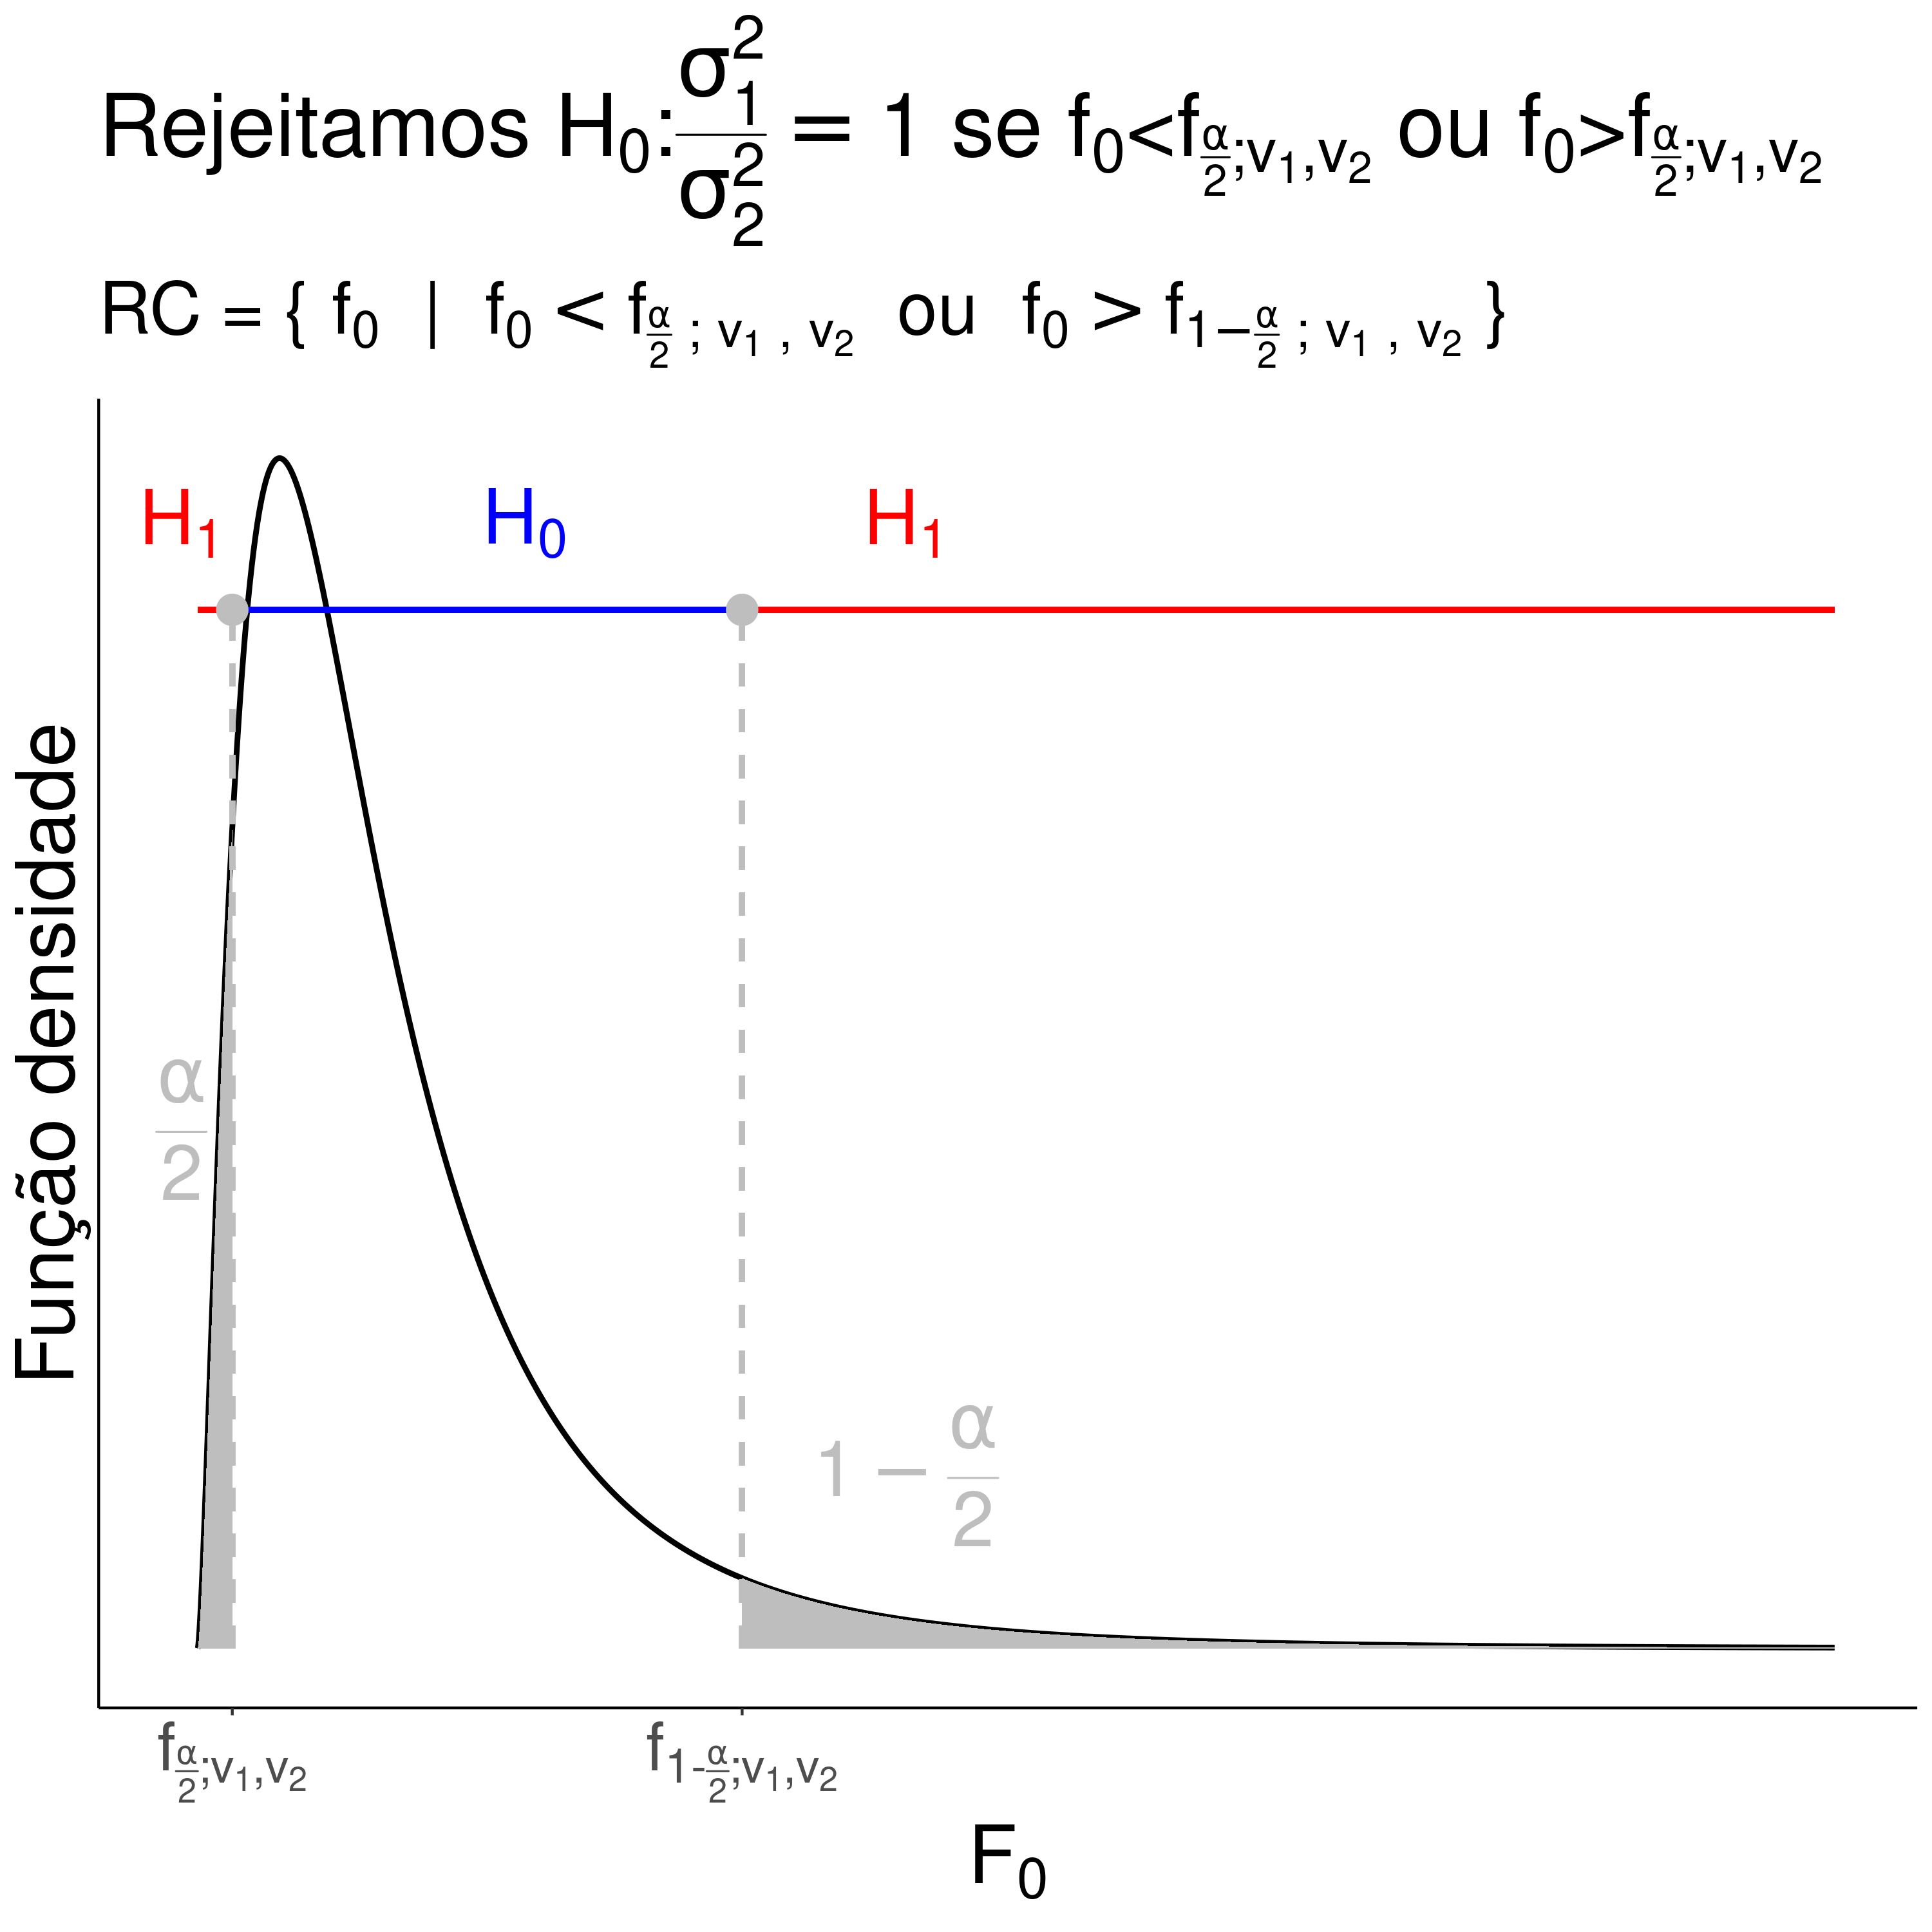
\includegraphics[width=0.32\linewidth]{figures/test-variance-bilateral.png} \label{fig:test-variance-bilateral}} \hfill
	\subfloat[][Teste bilateral.]{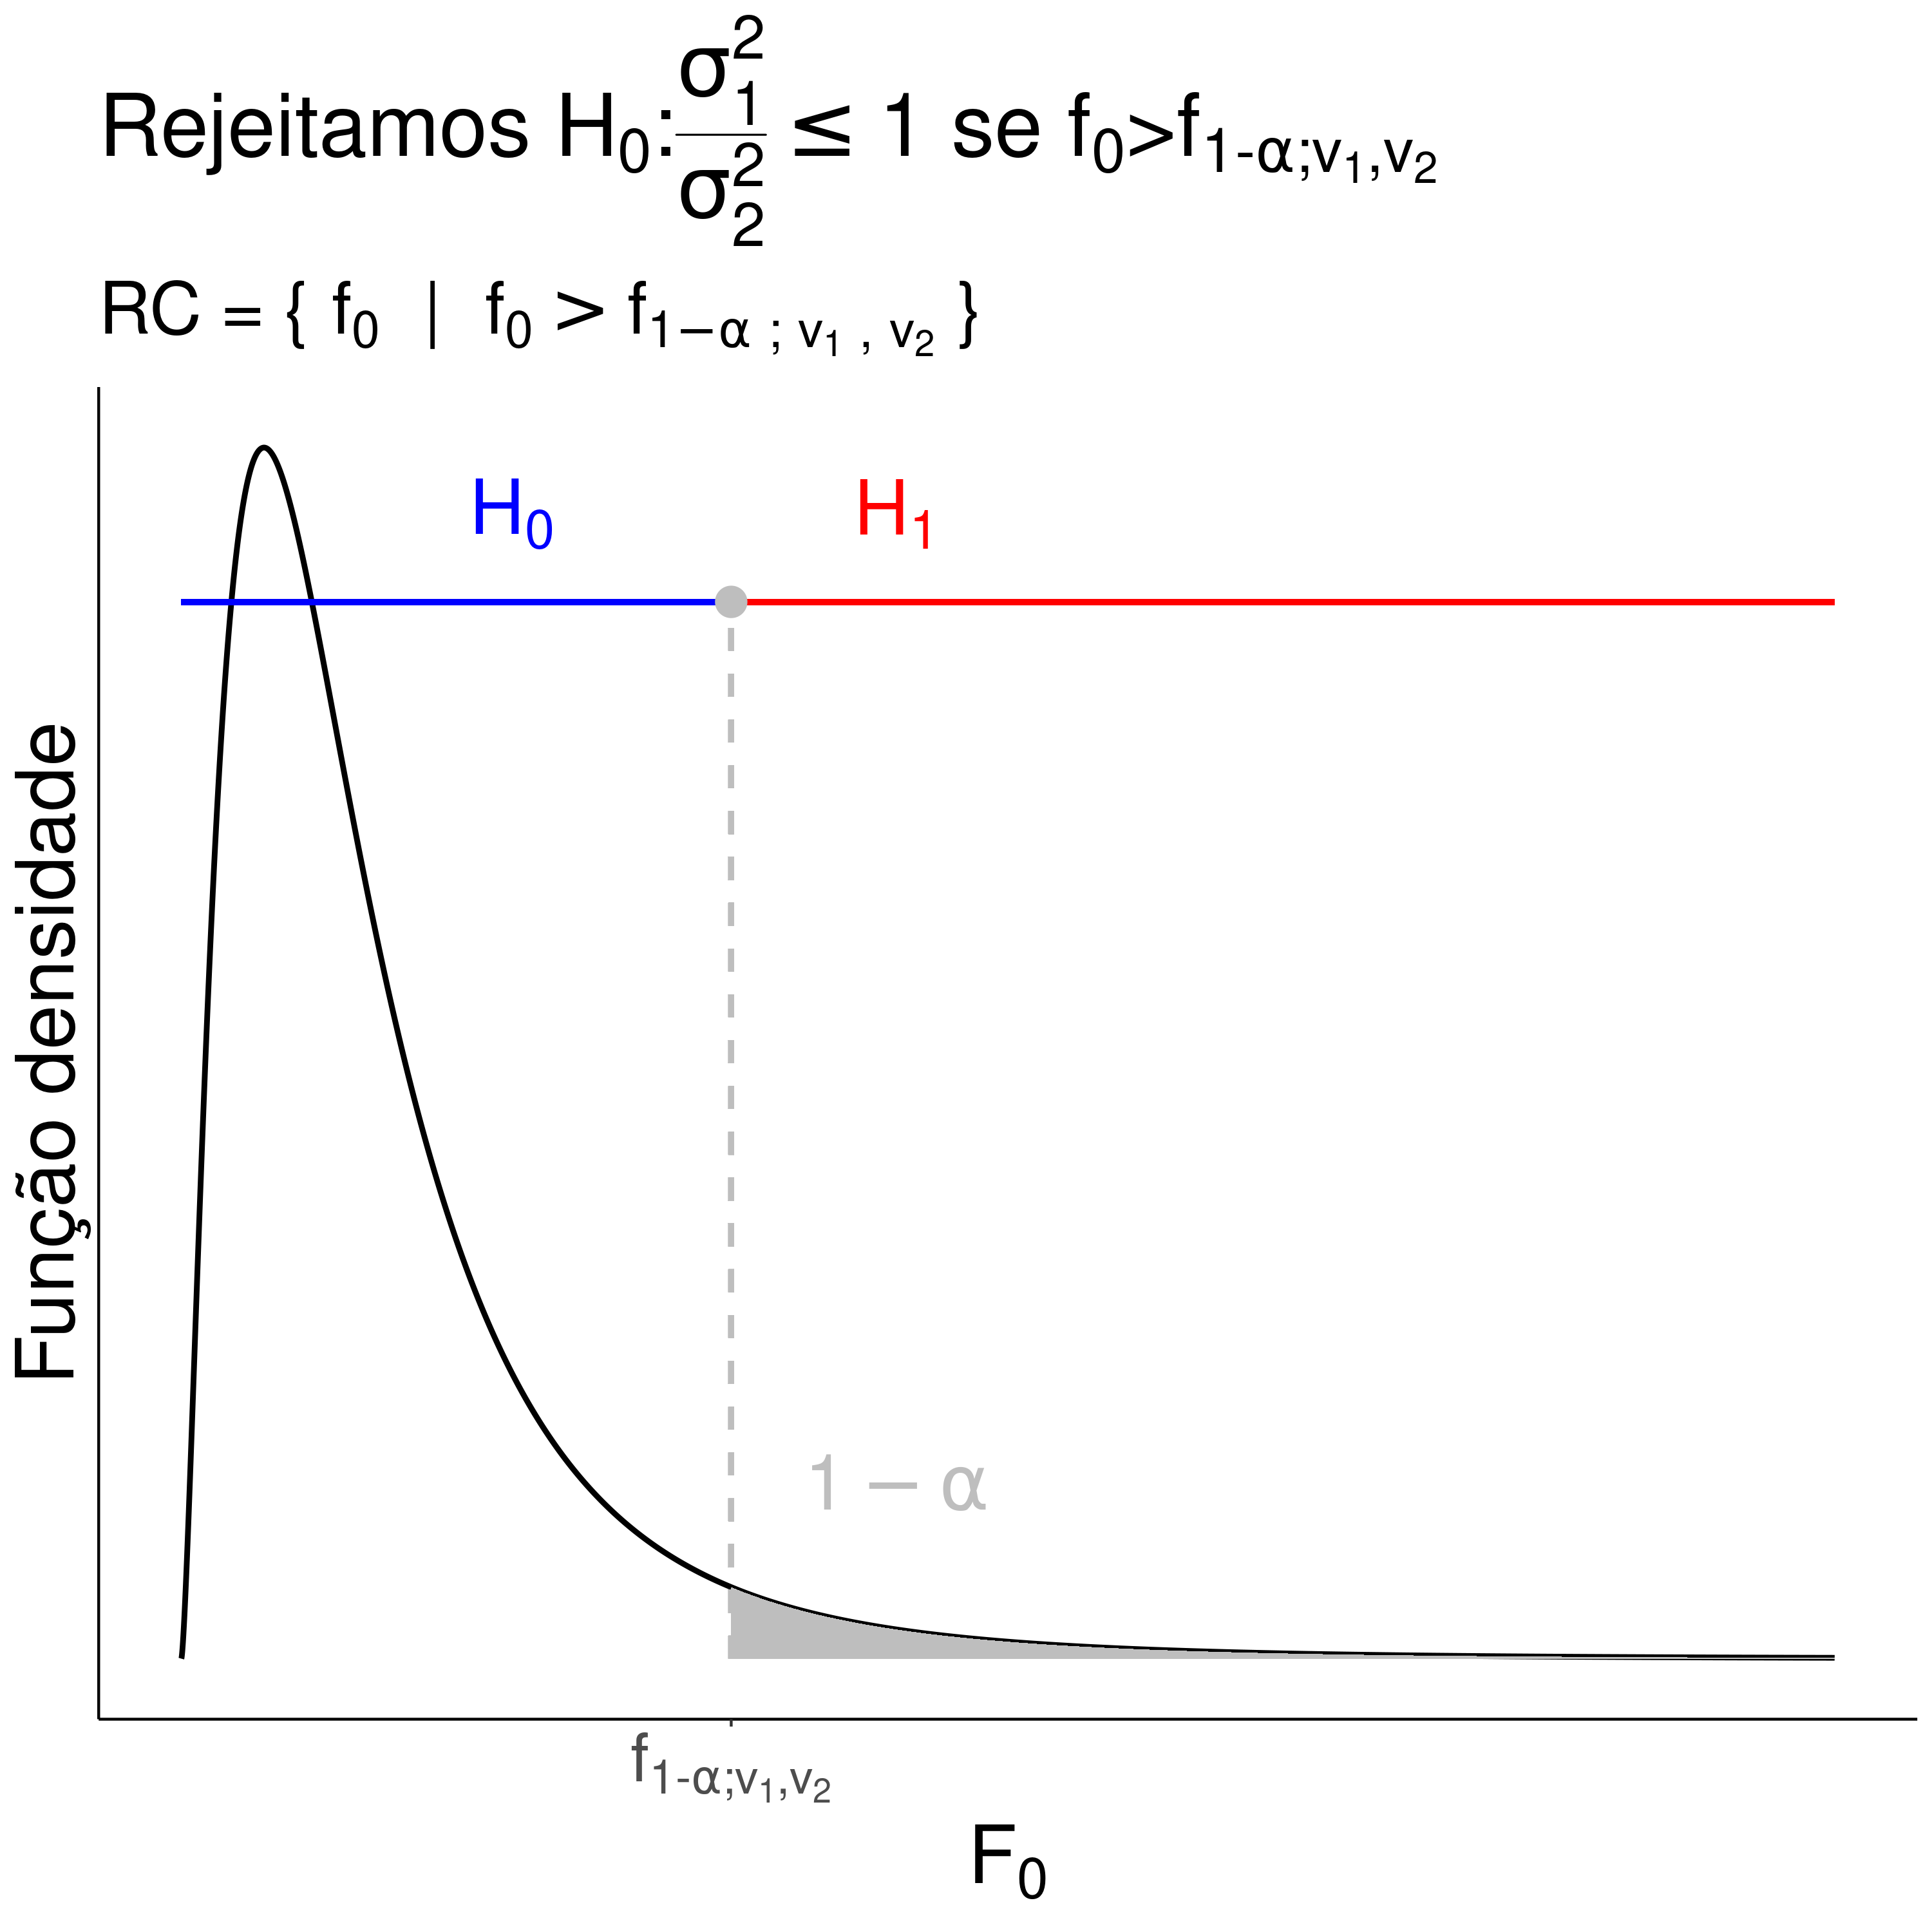
\includegraphics[width=0.32\linewidth]{figures/test-variance-unilateral-h1-upper.png} \label{fig:test-variance-unilateral-h1-upper}} \hfill
	\subfloat[][Teste bilateral.]{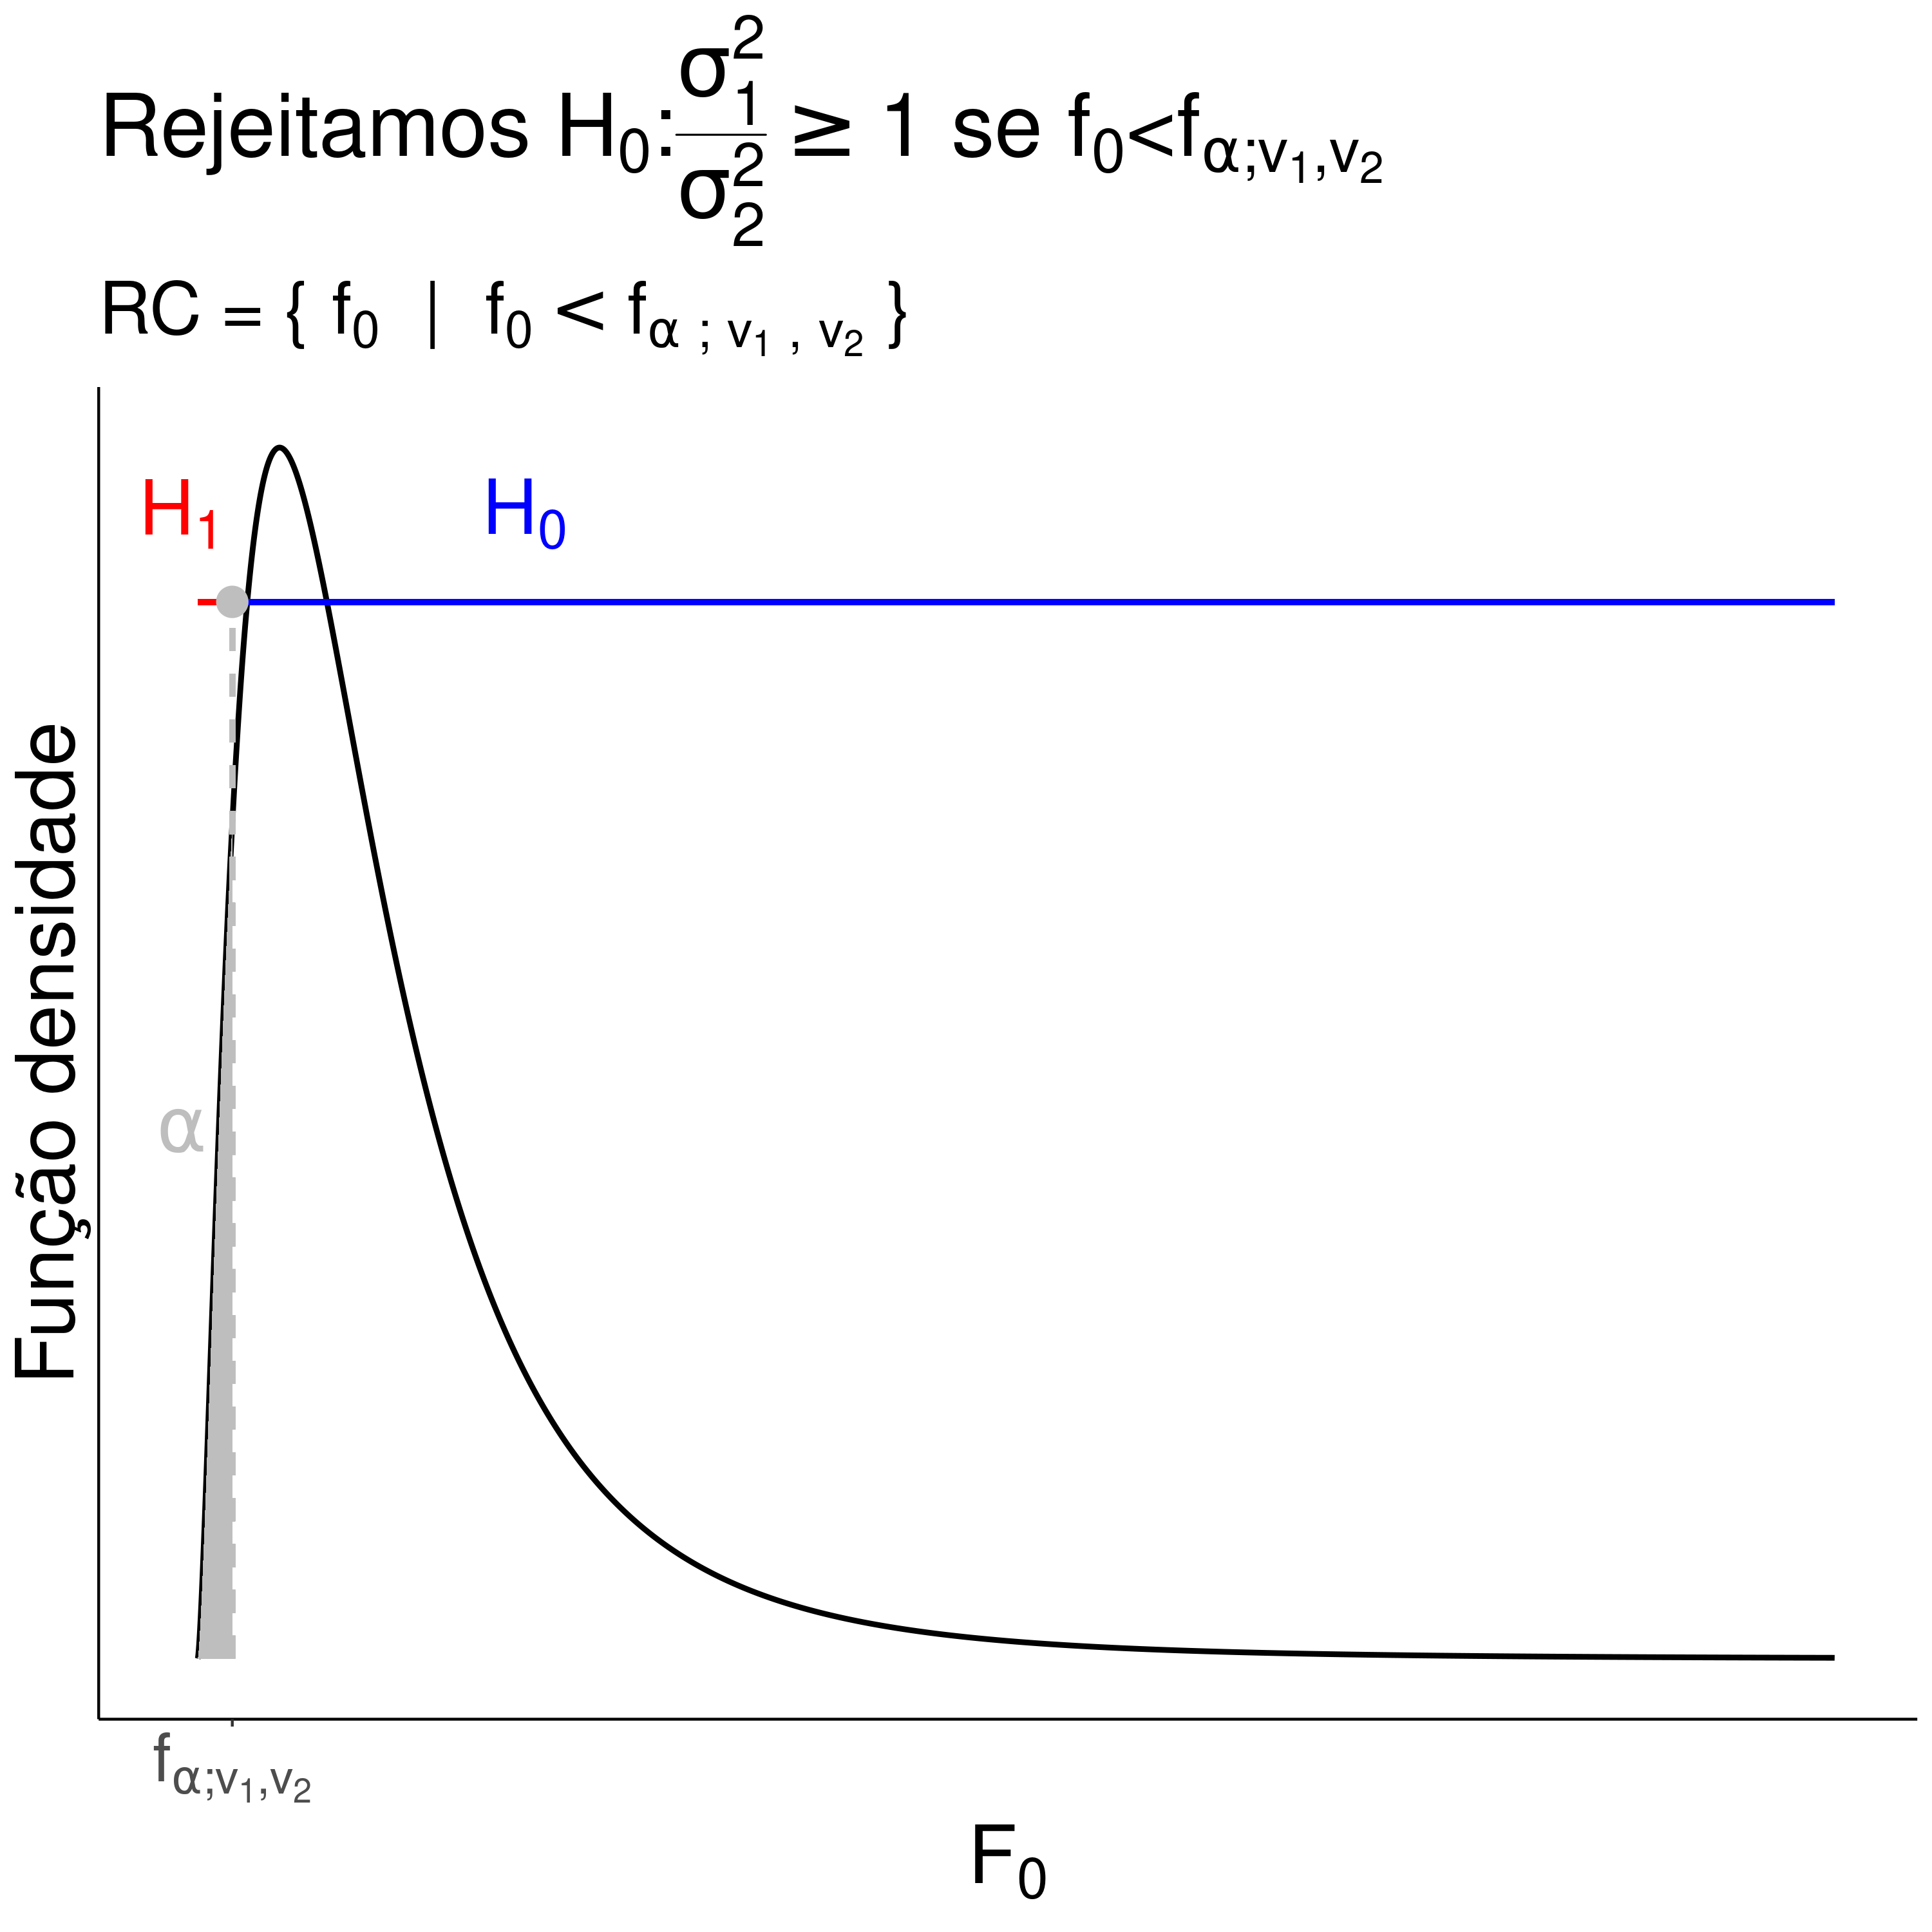
\includegraphics[width=0.32\linewidth]{figures/test-variance-unilateral-h1-lower.png} \label{fig:test-variance-unilateral-h1-lower}} 
	\caption{Região crítica para comparar variâncias de populações normais.}
\end{figure}
\end{frame}

\begin{frame}{Comparação de variâncias $\sigma_1^2$ e $\sigma_2^2$ de duas populações normais.}

\begin{itemize}
	\item Na Figura~\ref{fig:test-variance-bilateral}, testamos $H_0: \frac{\sigma_1^2}{\sigma_2^2} = 1$ versus $H_1: \frac{\sigma_1^2}{\sigma_2^2} \neq 1$. Rejeitamos $H_0$ se $f_0 = \frac{s_1^2}{s_2^2} \in \allowbreak RC=\{f_0 \mid f_0 < f_{\frac{\alpha}{2};n_1-1, n_2-1} \mbox{ ou } f_0 > f_{1-\frac{\alpha}{2}; n_1-1, n_2-1} \}$, em que $P\left( F_{n_1-1, n_2-1} \leq f_{\frac{\alpha}{2};n_1-1, n_2-1} \right) = \frac{\alpha}{2}$ e $P\left(F_{n_1-1, n_2-1} \leq  f_{1-\frac{\alpha}{2};n_1-1, n_2-1} \right) = 1- \frac{\alpha}{2}$;
	\vfill
	
	\item Na Figura~\ref{fig:test-variance-unilateral-h1-upper}, testamos $H_0: \frac{\sigma_1^2}{\sigma_2^2} \leq 1$ versus $H_1: \frac{\sigma_1^2}{\sigma_2^2} > 1$. Rejeitamos $H_0$ se $f_0 = \frac{s_1^2}{s_2^2}  \in \allowbreak RC=\{f_0 \mid f_0 > f_{1-\alpha; n_1-1, n_2-1}  \}$, em que $P\left(F_{n_1-1, n_2-1} \leq  f_{1-\alpha;n_1-1, n_2-1} \right) =1- \alpha$;
	\vfill
	
	\item Na Figura~\ref{fig:test-variance-unilateral-h1-lower}, testamos $H_0: \frac{\sigma_1^2}{\sigma_2^2} \geq 1$ versus $H_1: \frac{\sigma_1^2}{\sigma_2^2} < 1$. Rejeitamos $H_0$ se $f_0 = \frac{s_1^2}{s_2^2} \in \allowbreak RC=\{f_0 \mid f_0 < f_{\alpha;n_1-1, n_2-1}  \}$, em que $P\left(F_{n_1-1, n_2-1} \leq f_{\alpha;n_1-1, n_2-1} \right) = \alpha$.
\end{itemize}
Chamamos $f_{\alpha; n_1-1, n_2-1}$, $f_{1-\alpha;n_1, n_2}$, $f_{\frac{\alpha}{2}; n_1-1, n_2-1}$ e $f_{1-\frac{\alpha}{2}; n_1-1, n_2-1}$ são chamados de valores críticos.

\end{frame}

\begin{frame}{Comparação de variâncias $\sigma_1^2$ e $\sigma_2^2$ de duas populações normais.}

\large
\begin{block}{Exemplo}
	Um estudo foi realizado para determinar se homens e mulheres diferem na repetibilidade na montagem de componentes em placas de circuito impresso. Amostras de 25 homens e 21 mulheres foram selecionadas, e o tempo de montagem do circuito impresso foi mensurado. 
	O desvio padrão de tempo de montagem foram $s_{\tiny \mbox{homens}} = 1,25$ minutos e $s_{\tiny \mbox{mulheres}} = 0,75$ minutos. Existe evidência estatística de que a repetibilidade entre homens e mulheres são diferentes ao nível de significância de $\alpha=5\%$? Calcule o valor-p.
\end{block}
 
\normalsize
 \end{frame}

\begin{frame}{Comparação de variâncias $\sigma_1^2$ e $\sigma_2^2$ de duas populações normais.}

\small

\begin{block}{Solução}
	\textbf{Passo 1)} Queremos testar as hipóteses: $H_0: \frac{\sigma_1^2}{\sigma_2^2} = 1$ e $H_1: \frac{\sigma_1^2}{\sigma_2^2} \neq 1$;
	
	\textbf{Passo 2)} Nível de significância $\alpha=5\%$;
	
	\textbf{Passo 3)} Rejeito $H_0$ se $f_0 = \frac{s_1^2}{s_2^2}$ for grande ou for pequeno. Ou seja, $RC=\left\{
	 f_0 \mid f_0 < f_{\frac{\alpha}{2}; n_1-1, n_2-1} \mbox{ ou } f_{1-\frac{\alpha}{2}; n_1-1, n_2-1} < f_0 \right\}$;
	 
	 \textbf{Passo 4)} Vamos encontrar os valores críticos:
	 \begin{itemize}
	 	\item $P(F_{n_1-1, n_2-1} \leq f_{1-\frac{\alpha}{2}; n_1-1, n_2-1}) = P(F_{n_1-1, n_2-1} \leq f_{0,975; 24, 20}) = 1- \frac{\alpha}{2}= 0,975$, então $f_{0,975; 24, 20} = 2,756$;
	 	\item $P(F_{n_2-1, n_1-1} \leq f_{1-\frac{\alpha}{2}; n_2-1, n_1-1}) = P(F_{n_2-1, n_1-1} \leq f_{0,975; 20, 24}) = 1- \frac{\alpha}{2}= 0,975$, então $f_{0,975; 20, 24} = 2,327$;
	 	\item $f_{\frac{\alpha}{2}; n_1-1, n_2-1} = f_{0,025; 24, 20} = \frac{1}{f_{1-\frac{\alpha}{2}; n_2-1, n_1-1}} = \frac{1}{2,237} = 0,4297$.
	 \end{itemize}
 
 	\textbf{Passo 5)} Como $s_1=1,25$, $s_2=0,75$ e $f_0 = \frac{s_1^2}{s_2^2} = \frac{1,25^2}{0,75^2} = 2,7778 \in RC$, então rejeitamos $H_0$.
 	
 	Ou seja, ao nível de significância $\alpha=5\%$, homens e mulheres não tem a mesma repetibilidade.
\end{block}

\normalsize

\end{frame}

\begin{frame}{Comparação de variâncias $\sigma_1^2$ e $\sigma_2^2$ de duas populações normais.}

\begin{block}{Solução (valor-p)}

O valor-p é calculado através de 
$$p = 2\cdot \min \left( P(F_{v_1, v_2} \leq f_0), P(F_{v_1, v_2} \geq f_0)  \right).$$


\begin{figure}[htbp]
		\centering
		\subfloat[][$F_0$ pequeno.]{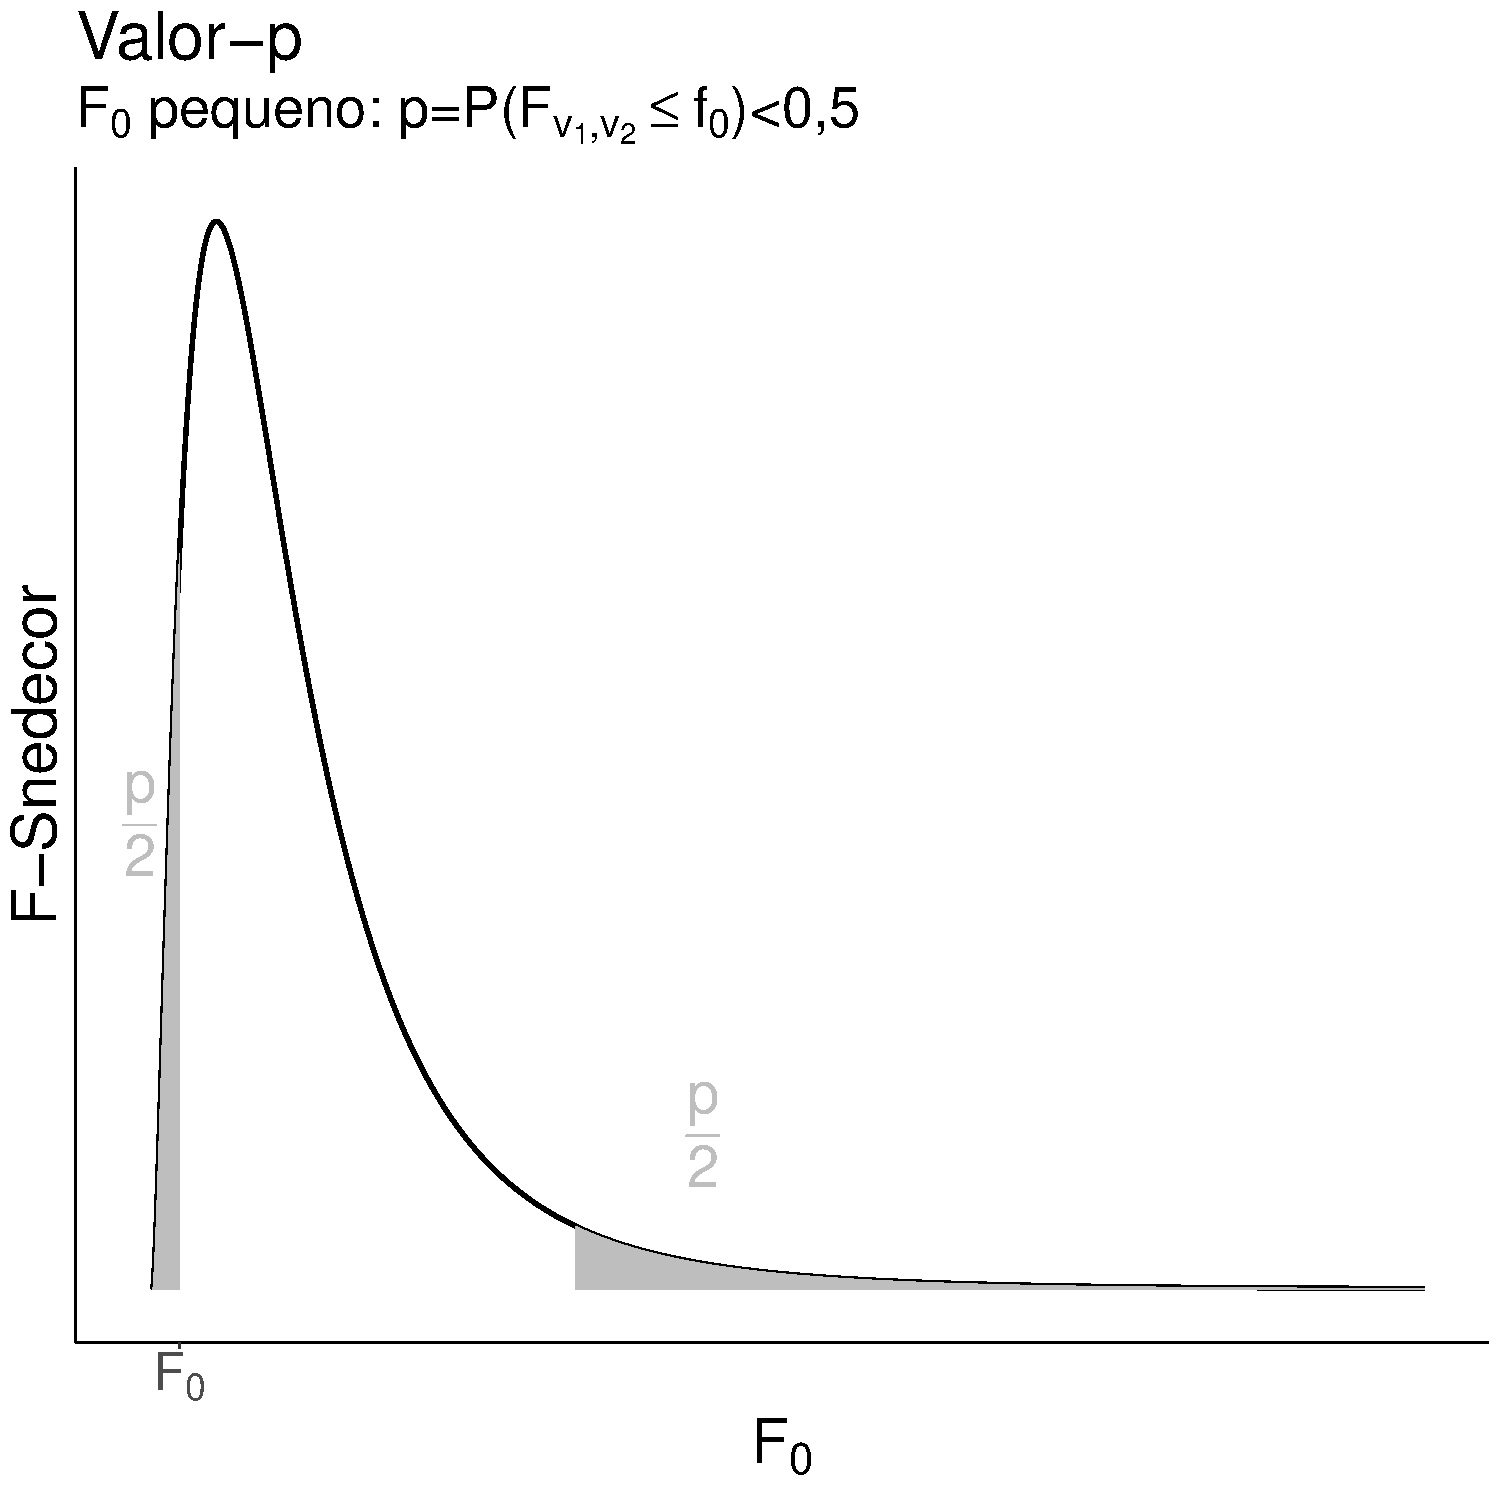
\includegraphics[width=0.45\linewidth]{figures/test-variance-valor-p-1.pdf} \label{fig:test-variance-valor-p-1}}
		\subfloat[][ $F_0$ grande.]{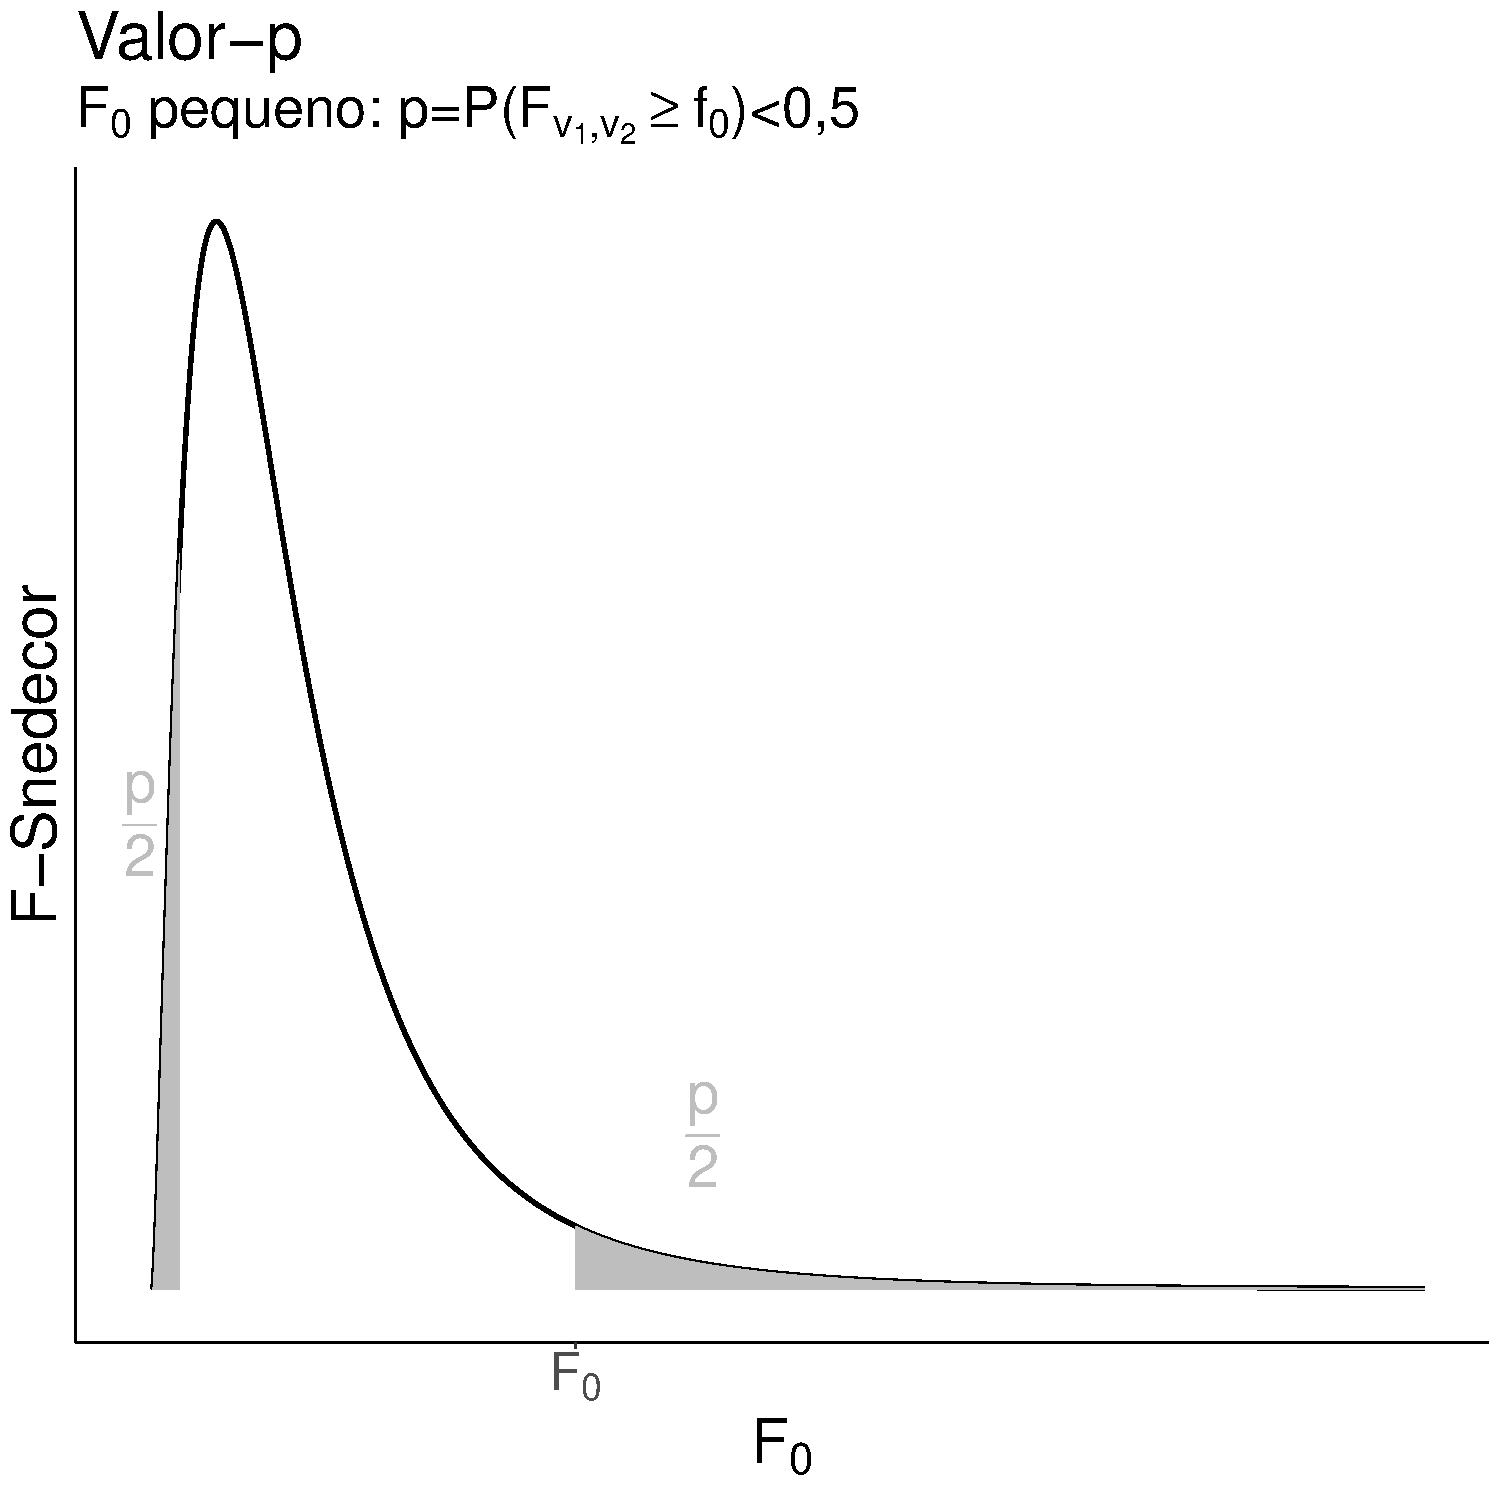
\includegraphics[width=0.45\linewidth]{figures/test-variance-valor-p-2.pdf} \label{fig:test-variance-valor-p-2}}
		\caption{Valor-p depende se $P\left( F_{v_1, v_2} \leq F_0 \right)< 0,5$ ou se $P\left( F_{v_1, v_2} \geq F_0 \right) < 0,5$.}
\end{figure}

\end{block}

\end{frame}

\begin{frame}{Comparação de variâncias $\sigma_1^2$ e $\sigma_2^2$ de duas populações normais.}

\begin{block}{Solução}
	O valor-p é calculado através de
	$$p = 2 \cdot \min \left( P\left( F_{v_1, v_2} \leq f_0 \right); P\left( F_{v_1, v_2} \geq f_0 \right) \right).$$
	
	Como $n_1=25$, $n_2=21$, $s_1 = 1,25$, $s_2=0,75$ e $F_0 = \frac{s_1^2}{s_2^2} = \frac{1,25^2}{0,75^2} = 2,78$, então 
	\begin{itemize}
		\item $P\left( F_{n_1-1, n_2-1} \leq f_0 \right) = P\left( F_{24, 20} \leq 2,78 \right) = 0,9883$;
		\item $P\left( F_{n_1-1, n_2-1} \geq f_0 \right) =1 -  P\left( F_{24, 20} \leq 2,78 \right) =1- 0,9883 = 0,0117$.
	\end{itemize}

	Então, o valor-p está calculado através de
	\begin{align*}
		p &= 2 \cdot \min \left( P\left( F_{v_1, v_2} \leq f_0 \right); P\left( F_{v_1, v_2} \geq f_0 \right) \right)\\
		&= 2 \cdot \min(0,9883; 0,0117)\\
		&= 0,0234.
	\end{align*}
	
	Como $p=0,0234 < 0,05=\alpha$, rejeitamos $H_0$ e homens e mulheres não teremos a repetibilidade.
\end{block}
\end{frame}

\begin{frame}{Comparação de variâncias $\sigma_1^2$ e $\sigma_2^2$ de duas populações normais.}

\large

\begin{block}{Exemplo}
	Os pontos de fusão de duas ligas usadas na formulação de solda foram investigados por $21$ amostras de fusão de cada material. Obtemos $s_1=4^\circ F$  e $s_2=3^\circ F$. Existe evidência de que a variabilidade do ponto de fusão da segunda liga é menor que a variabilidade do ponto de fusão da primeira liga ao nível de significância $\alpha=5\%$? Calcule o valor-p. 
\end{block}

\normalsize

\end{frame}

\begin{frame}{Comparação de variâncias $\sigma_1^2$ e $\sigma_2^2$ de duas populações normais.}

\begin{block}{Solução}
	\textbf{Passo 1)} Queremos testar as hipóteses: $H_0: \frac{\sigma_1^2}{\sigma_2^2} \leq 1$ e $H_1: \frac{\sigma_1^2}{\sigma_2^2}  > 1$;
	
	\textbf{Passo 2)} Nível de significância $\alpha=5\%$;
	
	\textbf{Passo 3)} Rejeitamos $H_0$ se $f_0 = \frac{s_1^2}{s_2^2}$ for grande. Ou seja, $RC=\left\{ f_0 \mid f_0 > f_{1-\alpha; n_1-1, n_2-1} \right\}$;
	
	\textbf{Passo 4)} Vamos encontrar o valor crítico:
	\begin{itemize}
		\item $P\left( F_{n_1-1, n_2-1} \leq f_{1-\alpha; n_1-1, n_2-1} \right) = P\left( F_{20, 20} \leq f_{0,95; 20, 20} \right) = 1-\alpha=0,95$, então $f_{0,95; 20, 20} = 1,7938$.
	\end{itemize}

	\textbf{Passo 5)} Como $s_1 = 4$, $s_2=3$ e $f_0 = \frac{s_1^2}{s_2^2} = 1,78 \not\in RC$, e não rejeitamos $H_0$, ou seja, não existe evidência de que o ponto de fusão da segunda liga é menor de que o ponto de fusão da primeira liga.
\end{block}

\end{frame}

\begin{frame}{Comparação de variâncias $\sigma_1^2$ e $\sigma_2^2$ de duas populações normais.}

\begin{block}{Solução (valor-p)}
	O valor-p é calculado através de 
	$$p=P\left( F_0 > f_0 \mid H_0 \right) =1- P\left( F_{n_1-1, n_2-1} \leq f_0  \right),$$
	em que $f_0$ é o valor observador da estatística.
	
	Como $s_1 = 4$, $s_2 = 3$, $n_1=n_2=21$ e $f_0 = \frac{s_1^2}{s_2^2}=\frac{4^2}{3^2} = 1,78$, então
	\begin{align*}
		p &= 1 - P \left( F_{n_1-1, n_2-1} \leq f_0 \right)\\
		&=1- P \left( F_{20, 20} \leq 1,78 \right)\\
		&= 1 - 0,8970\\
		&= 0,103.
	\end{align*}
	
	Como $p=0,103 > \alpha = 0,05$, não rejeitamos $H_0$. Ou seja, ao nível de significância $\alpha=5\%$, não existe evidência de variabilidade do ponto de fusão da segunda liga é menor do que o ponto de fusão da primeira liga.
\end{block}

\end{frame}

\begin{frame}{Comparação de variâncias $\sigma_1^2$ e $\sigma_2^2$ de duas populações normais.}

\begin{block}{Exemplo}
	Imagine que temos duas variáveis aleatórias contínuas com distribuição normal e independentes. Um pesquisador coletou $26$ valores da primeira variável e $21$ valores da segunda variável. Algumas informações desse experimento está na Tabela~\ref{tab:test-variance-h1-lower}. Imagine que queremos decidir entre duas hipóteses $H_0: \frac{\sigma_1^2}{\sigma_2^2} \geq 1$ e $H_1: \frac{\sigma_1^2}{\sigma_2^2} < 1$. Complete a Tabela~\ref{tab:test-variance-h1-lower}. Ao nível de significância $\alpha=5\%$, qual foi a decisão do pesquisador? Calcule o valor-p.
	\begin{table}[htbp]
		\centering
		\begin{tabular}{c|c|c|c}
			\toprule[0.05cm]
			$\alpha$ & $f_0$ & valor-p & $s_1$\\
			\midrule[0.025cm]
			$5\%$ & & & $5,21$ \\
			\midrule[0.05cm]
			$s_2$ & Decisão & $n_1$ & $n_2$\\ \midrule[0.025cm]
			$13,38$ & & $26$ & $21$\\
			\bottomrule[0.05cm]
		\end{tabular}
		\caption{Algumas informações do experimento.}
		\label{tab:test-variance-h1-lower}
	\end{table}
\end{block}
\end{frame}

\begin{frame}{Comparação de variâncias $\sigma_1^2$ e $\sigma_2^2$ de duas populações normais.}

\begin{block}{Solução}
	\textbf{Passo 1)} Queremos testar as seguintes hipóteses: $H_0: \frac{\sigma_1^2}{\sigma_2^2} \geq 1$ e $H_1: \frac{\sigma_1^2}{\sigma_2^2} < 1$;
	
	\textbf{Passo 2)} Nível de significância $\alpha=5\%$;
	
	\textbf{Passo 3)} Rejeito $H_0$ se $f_0 = \frac{s_1^2}{s_2^2}$ for pequeno. Ou seja, $RC=\left\{ f_0 \mid f_0 < f_{\alpha; n_1-1, n_2-1} \right\}$;
	
	\textbf{Passo 4)} Vamos encontrar o valor crítico. Note que $f_{\alpha; n_1-1, n_2-1} = \frac{1}{f_{1-\alpha; n_2-1, n_1-1}}$, em que
	\begin{itemize}
		\item $P\left(F_{n_2-1, n_1-1} \leq f_{1-\alpha;n_2-1, n_1-1} \right) = P\left(F_{25, 20} \leq f_{0,95;20, 25} \right) = 1-\alpha=0,95$, então $f_{0,95;20, 25} = 2,0075$;
	\end{itemize}
	Então, $f_{0,05; 25, 20} = \frac{1}{2,0075} = 0,4981$.
	
	\textbf{Passo 5)} Como $s_1 = 5,21$, $s_2 = 13,38$ e $f_0 = \frac{s_1^2}{s_2^2} = \frac{5,21^2}{13,38^2} = 0,1516 \in RC$, então rejeitamos $H_0$ ao nível de significância $\alpha=5\%$.
	
\end{block}
\end{frame}

\begin{frame}{Comparação de variâncias $\sigma_1^2$ e $\sigma_2^2$ de duas populações normais.}

\begin{block}{Solução (valor-p)}
	O valor-p é calculado através de
	$$p=P\left( F_0 < f_0 \mid H_0 \right) = P\left( F_{n_1-1, n_2-1} < f_0 \right),$$
	em que $f_0 = \frac{s_1^2}{s_2^2}$ calculado usando a  nossa amostra.
	
	Como $s_1=5,21$, $s_2 = 13,38$ e $f_0 = \frac{s_1^2}{s_2^2} = \frac{5,21^2}{13,38^2} = 0,1516$, o valor-p é dado por
	\begin{align*}
		p &= P\left( F_{n_1-1, n_2-1} < f_0 \right)\\
		&= P\left(F_{25, 20} < 0,1516\right)\\
		&= 0
	\end{align*}
	
	Como $p=0<\alpha=0,05$, rejeitamos $H_0$ ao nível de significância $\alpha=5\%$.
\end{block}
\end{frame}

\subsection{Poder e tamanho da amostra.}

\begin{frame}{Poder do teste: $H_0:\frac{\sigma_1^2}{\sigma_2^2} = 1$ e $H_1:\frac{\sigma_1^2}{\sigma_2^2} \neq 1$.}

\small

Imagine que
\begin{itemize}
	\item Hipóteses: $H_0:\frac{\sigma_1^2}{\sigma_2^2} = 1$ e $H_1:\frac{\sigma_1^2}{\sigma_2^2} \neq 1$;
	\item $H_1$ é verdade e conhecemos a razão $\lambda=\frac{\sigma_1}{\sigma_2} \neq 1$;
	\item $F_0 = \frac{s_1^2}{s_2^2}$ e $F_0 \frac{\sigma_2^2}{\sigma_1^2}=  \frac{F_0}{\lambda^2} \sim F_{n_1-1, n_2-1}$;
	\item Ao nível de significância $\alpha$, temos $RC = \left\{ f_0 \mid f_0 < f_{\frac{\alpha}{2}; n_1-1, n_2-1} \mbox{ ou } f_{1-\frac{\alpha}{2}; n_1-1, n_2-1} < f_0 \right\}$.
\end{itemize}
\vfill	

Poder do teste é dado
\begin{align*}
\textcolor{important}{1-\beta} &=1 - P\left( f_{\frac{\alpha}{2}; n_1-1, n_2-1} \leq F_0  \leq f_{1-\frac{\alpha}{2}; n_1-1, n_2-1} \mid H_1\right)\\
&= 1 - P \left(F_{n_1-1, n_2-1} \leq f_{1-\frac{\alpha}{2};n_1-1, n_2-1} \frac{1}{\lambda^2} \right) + P \left(F_{n_1-1, n_2-1} \leq f_{\frac{\alpha}{2};n_1-1, n_2-1} \frac{1}{\lambda^2} \right)
\end{align*}
\vfill

A \textcolor{important}{Função Poder}, dado o tamanho da amostra $n$, é uma função das médias populacionais na hipótese alternativa  $\pi: (0,\infty) - \{1\} \longrightarrow [0,1]$ dada por
\begin{align*}
\pi(\lambda) = 1 - P \left(F_{n_1-1, n_2-1} \leq f_{1-\frac{\alpha}{2};n_1-1, n_2-1} \frac{1}{\lambda^2} \right) + P \left(F_{n_1-1, n_2-1} \leq f_{\frac{\alpha}{2};n_1-1, n_2-1} \frac{1}{\lambda^2} \right).
\end{align*}
em que $\lambda = \frac{\sigma_1}{\sigma_2} \in (0, \infty)- \{1\}$. Alguns livros chamada a Função Poder de \textcolor{important}{Curva de Característica Operacional.}

\normalsize

\end{frame}

\begin{frame}[fragile]{Tamanho da amostra: $H_0:\frac{\sigma_1^2}{\sigma_2^2} = 1$ e $H_1:\frac{\sigma_1^2}{\sigma_2^2} \neq 1$.}
\small

Imagine que
\begin{itemize}
	\item Hipóteses: $H_0:\frac{\sigma_1^2}{\sigma_2^2} = 1$ e $H_1:\frac{\sigma_1^2}{\sigma_2^2} \neq 1$;
	\item $H_1$ é verdade e conhecemos a razão $\lambda=\frac{\sigma_1}{\sigma_2} \neq 1$;
	\item $F_0 = \frac{s_1^2}{s_2^2}$ e $F_0 \frac{\sigma_2^2}{\sigma_1^2} =  \frac{F_0}{\lambda^2} \sim F_{n_1-1, n_2-1}$;
	\item Ao nível de significância $\alpha$, temos $RC = \left\{ f_0 \mid f_0 < f_{\frac{\alpha}{2}; n_1-1, n_2-1} \mbox{ ou } f_{1-\frac{\alpha}{2}; n_1-1, n_2-1} < f_0 \right\}$.
\end{itemize}
\vfill


Imagine que conhecemos $\sigma_1$, $\sigma_2$, $\lambda = \frac{\sigma_1}{\sigma_2}$, $\alpha$, $1-\beta$ e suponha que $n=n_1=n_2$, então o tamanho \sout{mínimo} das amostras das variáveis é solução da equação
\scriptsize
\begin{align}\label{eq:pwr-f-test-bilateral}
1-\beta=1 - P \left(F_{n-1, n-1} \leq f_{1-\frac{\alpha}{2};n-1, n-1} \frac{1}{\lambda^2} \right) + P \left(F_{n-1, n-1} \leq f_{\frac{\alpha}{2};n-1, n-1} \frac{1}{\lambda^2} \right).
\end{align}


A equação~\eqref{eq:pwr-f-test-bilateral} é resolvida usando métodos numéricos que estão implementados em diversos \textit{softwares}.
\begin{description}
	\item[No R] \lstinline|pwr_sigma_2pop|
\end{description}
Esta função está no pacote \lstinline|power|, que pode ser instalado usando o pacote \lstinline|devtools|: \lstinline|devtools::install_github("gilberto-sassi/power")|.

\normalsize
\end{frame}

\begin{frame}{Poder do teste: $H_0:\frac{\sigma_1^2}{\sigma_2^2} = 1$ e $H_1:\frac{\sigma_1^2}{\sigma_2^2} \neq 1$.}

\large

\begin{block}{Exemplo}
	Um estudo foi realizado para determinar se homens e mulheres diferem na repetibilidade na montagem de componentes em placas de circuito impresso. Amostras de 25 homens e 21 mulheres foram selecionadas, e o tempo de montagem do circuito impresso foi mensurado. 
	Imagine que $\sigma_1=15$ segundos e $\sigma_2=25$ segundos. Ao nível de significância $\alpha=5\%$, qual o poder do teste?
\end{block}

\normalsize
\end{frame}

\begin{frame}[fragile]{Poder do teste: $H_0:\frac{\sigma_1^2}{\sigma_2^2} = 1$ e $H_1:\frac{\sigma_1^2}{\sigma_2^2} \neq 1$.}

\tiny

\begin{block}{Solução}
	\textbf{Passo 1)} Queremos testar as hipóteses: $H_0: \frac{\sigma_1}{\sigma_2} = 1$ e $H_1: \frac{\sigma_1}{\sigma_2}$;
	
	\textbf{Passo 2)} Nível de significância $\alpha=5\%$;
	
	Note que $\lambda = \frac{\sigma_1}{\sigma_2} = \frac{15}{25}$, $n_1=25$, $n_2=21$, $\alpha=5\%$.
	
	Primeiro vamos encontrar os quantis da distribuição $F$-Snedecor:
	\begin{itemize}
		\item $P\left(F_{n_1-1, n_2-1} \leq f_{1-\frac{\alpha}{2}; n_1-1, n_2-1} \right) = P\left(F_{24, 20} \leq f_{0,975; 24, 20} \right) =1- \frac{\alpha}{2} = 0,975$, então $f_{0,975; 24, 20} = 2,408$;
		\item $P\left(F_{n_2-1, n_1-1} \leq f_{1-\frac{\alpha}{2}; n_2-1, n_1-1} \right) = P\left(F_{20, 24} \leq f_{0,975; 20, 24} \right) =1- \frac{\alpha}{2} = 0,975$, então $f_{0,975; 20, 24} = 2,327$;
		\item $f_{\frac{\alpha}{2}; 24, 20} = f_{0,025; 24, 20} =  \frac{1}{f_{1-\frac{\alpha}{2};20, 24}} = \frac{1}{2,327}=0,4297$.
	\end{itemize}

	Então o poder do teste é dado por
	\begin{align*}
		1-\beta &= 1 - P\left( F_{n_1-1, n_2-1} \leq f_{1-\frac{\alpha}{2};n_1-1, n_2-1} \frac{1}{\lambda^2} \right) + P\left( F_{n_1-1, n_2-1} \leq f_{\frac{\alpha}{2};n_1-1, n_2-1} \frac{1}{\lambda^2} \right)\\
%		&=1 - P\left( F_{24, 20} \leq f_{0,975;24, 20} \frac{1}{\lambda^2} \right) + P\left( F_{24, 20} \leq f_{0,025;24, 20} \frac{1}{\lambda^2} \right)\\
		&= 1 - P\left( F_{24, 20} \leq \frac{2,408 \cdot 25^2}{15^2} \right) + P\left( F_{24, 20} \leq \frac{0,4297 \cdot 25^2}{15^2} \right) = 0,6533.
	\end{align*}
\end{block}

\begin{lstlisting}[language = C, caption = Código no R.]
pwr_sigma_2pop(sigma1 = 15, sigma2 = 25, n1 = 25, n2 = 21, pwr = NULL,
		alternative = "two.sided", sig_level = 0.05)
\end{lstlisting}

\normalsize
\end{frame}

\begin{frame}{Tamanho da amostra: $H_0:\frac{\sigma_1^2}{\sigma_2^2} = 1$ e $H_1:\frac{\sigma_1^2}{\sigma_2^2} \neq 1$.}

\large

\begin{block}{Exemplo}
	Um estudo foi realizado para determinar se homens e mulheres diferem na repetibilidade na montagem de componentes em placas de circuito impresso. Amostras de homens e mulheres serão selecionadas, e o tempo de montagem do circuito impresso foi mensurado. 
	Imagine que $\sigma_1=15$ segundos e $\sigma_2=25$ segundos. Ao nível de significância $\alpha=5\%$e com poder do teste $1-\beta=99\%$, quantos homens e mulheres precisamos estudar?
\end{block}

\normalsize

\end{frame}


\begin{frame}[fragile]{Tamanho da amostra: $H_0:\frac{\sigma_1^2}{\sigma_2^2} = 1$ e $H_1:\frac{\sigma_1^2}{\sigma_2^2} \neq 1$.}

\small

\begin{block}{Solução}
	\textbf{Passo 1)} Queremos testar as hipóteses: $H_0: \frac{\sigma_1}{\sigma_2} = 1$ e $H_1: \frac{\sigma_1}{\sigma_2}$;
	
	\textbf{Passo 2)} Nível de significância $\alpha=5\%$;
	
		
	Note que $\lambda = \frac{\sigma_1}{\sigma_2} = \frac{15}{25}$, $\alpha=5\%$, $1-\beta=0,99$ e suponha que $n=n_1=n_2$, então a quantidade \sout{mínima} de homens e mulheres que precisamos estudar é solução da seguinte equação em $n$
	\begin{align*}
		1-\beta &= 1 - P\left( F_{n-1, n-1} \leq f_{1-\frac{\alpha}{2};n-1, n-1} \frac{1}{\lambda^2} \right) + P\left( F_{n-1, n-1} \leq f_{\frac{\alpha}{2};n-1, n-1} \frac{1}{\lambda^2} \right)\\
		&= 1 - P\left( F_{n-1, n-1} \leq f_{1-\frac{\alpha}{2};n-1, n-1} \frac{1}{\lambda^2} \right) + P\left( F_{n-1, n-1} \leq f_{\frac{\alpha}{2};n-1, n-1} \frac{1}{\lambda^2} \right) \\
		&= 1 - P\left( F_{n-1, n-1} \leq f_{0,975;n-1, n-1} \frac{25^2}{15^2} \right) + P\left( F_{n-1, n-1} \leq f_{0,025;n-1, n-1} \frac{25^2}{15^2} \right)
	\end{align*}
\end{block}

Então, precisamos estudar 73 homens e 73 mulheres.

\begin{lstlisting}[language = C, caption = Código no R.]
pwr_sigma_2pop(sigma1 = 15, sigma2 = 25, n1 = NULL, n2 = NULL,
				pwr = 0.99, alternative = "two.sided", sig_level = 0.05)
\end{lstlisting}

\normalsize

\end{frame}

\begin{frame}{Poder do teste: $H_0:\frac{\sigma_1^2}{\sigma_2^2} \leq 1$ e $H_1:\frac{\sigma_1^2}{\sigma_2^2} > 1$.}

\normalsize

Imagine que
\begin{itemize}
	\item Hipóteses: $H_0:\frac{\sigma_1^2}{\sigma_2^2} \leq 1$ e $H_1:\frac{\sigma_1^2}{\sigma_2^2} > 1$;
	\item $H_1$ é verdade e conhecemos a razão $\lambda=\frac{\sigma_1}{\sigma_2} > 1$;
	\item $F_0 = \frac{s_1^2}{s_2^2}$ e $F_0 \frac{\sigma_2^2}{\sigma_1^2} = \frac{F_0}{\lambda^2} \sim F_{n_1-1, n_2-1}$;
	\item Ao nível de significância $\alpha$, temos $RC = \left\{ f_0 \mid f_0 > f_{1-\alpha; n_1-1, n_2-1} \right\}$.
\end{itemize}
\vfill	

Poder do teste é dado
\begin{align*}
\textcolor{important}{1-\beta} &=1 - P\left( F_0 \leq f_{1-\alpha; n_1-1, n_2-1} \mid H_1\right)= 1 - P \left(F_{n_1-1, n_2-1} \leq f_{1-\alpha; n_1-1, n_2-1} \frac{1}{\lambda^2} \right)
\end{align*}
\vfill

A \textcolor{important}{Função Poder}, dado o tamanho da amostra $n$, é uma função das médias populacionais na hipótese alternativa  $\pi: (1,\infty) \longrightarrow [0,1]$ dada por
\begin{align*}
\pi(\lambda) = 1 - P \left(F_{n_1-1, n_2-1} \leq f_{1-\alpha; n_1-1, n_2-1} \frac{1}{\lambda^2} \right), \qquad \lambda = \frac{\sigma_1}{\sigma_2} \in (1, \infty).
\end{align*}
Alguns livros chamada a Função Poder de \textcolor{important}{Curva de Característica Operacional.}

\normalsize
\end{frame}

\begin{frame}{Tamanho da amostra: $H_0:\frac{\sigma_1^2}{\sigma_2^2} \leq 1$ e $H_1:\frac{\sigma_1^2}{\sigma_2^2} > 1$.}

\small

Imagine que
\begin{itemize}
\item Hipóteses: $H_0:\frac{\sigma_1^2}{\sigma_2^2} \leq 1$ e $H_1:\frac{\sigma_1^2}{\sigma_2^2} > 1$;
\item $H_1$ é verdade e conhecemos a razão $\lambda=\frac{\sigma_1}{\sigma_2} > 1$;
\item $F_0 = \frac{s_1^2}{s_2^2}$ e $F_0 \frac{\sigma_2^2}{\sigma_1^2} = \frac{F_0}{\lambda^2} \sim F_{n_1-1, n_2-1}$;
\item Ao nível de significância $\alpha$, temos $RC = \left\{ f_0 \mid f_0 > f_{1-\alpha; n_1-1, n_2-1}  \right\}$.
\end{itemize}
\vfill


Imagine que conhecemos $\sigma_1$, $\sigma_2$, $\lambda = \frac{\sigma_1}{\sigma_2}$, $\alpha$, $1-\beta$ e suponha que $n=n_1=n_2$, então o tamanho \sout{mínimo} das amostras das variáveis é solução da equação
\begin{align}\label{eq:pwr-f-test-greater}
1-\beta=1 - P \left(F_{n-1, n-1} \leq f_{1-\alpha; n-1, n-1} \frac{1}{\lambda^2} \right) = 1 - P \left(F_{n-1, n-1} \leq f_{1-\alpha; n-1, n-1} \frac{\sigma_2^2}{\sigma_1^2} \right).
\end{align}

A equação~\eqref{eq:pwr-f-test-greater} é resolvida usando métodos numéricos que estão implementados em diversos \textit{softwares}.
\begin{description}
	\item[No R] \lstinline|pwr_sigma_2pop|
\end{description}
Esta função está no pacote \lstinline|power|, que pode ser instalado usando o pacote \lstinline|devtools|: \lstinline|devtools::install_github("gilberto-sassi/power")|.

\normalsize
\end{frame}

\begin{frame}{Poder do teste: $H_0:\frac{\sigma_1^2}{\sigma_2^2} \leq 1$ e $H_1:\frac{\sigma_1^2}{\sigma_2^2} > 1$.}

\large
\begin{block}{Exemplo}
	Os pontos de fusão de duas ligas usadas na formulação de solda foram investigados por $21$ amostras de fusão de cada material. Assuma que $\sigma_1=10^\circ F$ e $\sigma_2=5^\circ F$. Um pesquisador deseja certificar que a variabilidade do ponto de fusão da segunda liga é menor que a variabilidade do ponto de fusão da primeira liga. Ao nível de significância $\alpha=5\%$, qual o poder do teste?
\end{block}

\normalsize
\end{frame}

\begin{frame}[fragile]{Poder do teste: $H_0:\frac{\sigma_1^2}{\sigma_2^2} \leq 1$ e $H_1:\frac{\sigma_1^2}{\sigma_2^2} > 1$.}

\begin{block}{Solução}
	\textbf{Passo 1)} Queremos testar as hipóteses: $H_0: \frac{\sigma_1^2}{\sigma_2^2} \leq 1$ e $H_1: \frac{\sigma_1^2}{\sigma_2^2} > 1$;
	
	\textbf{Passo 2)} Nível de significância $\alpha=5\%$;
	
	Note que $\sigma_1=10$, $\sigma_2=5$, $n=n_1=n_2=21$, $\alpha=0,05$..
	
	Primeiro vamos encontrar o quantil da distribuição $F$-Snedecor:
	\begin{itemize}
		\item $P( F_{n_1-1, n_2-1} \leq f_{1-\alpha; n_1-1, n_2-1} ) = P\left( F_{20, 20} \leq f_{0,95; 20, 20} \right) = 1-\alpha = 0,95$, então $f_{0,95; 20, 20} = 2,1242$.
	\end{itemize}

	Então o poder do teste é dado por
	\begin{align*}
		1-\beta &= 1- P \left( F_{20, 20} \leq f_{0,95; 20, 20} \frac{\sigma_2^2}{\sigma_1^2} \right) = 1- P \left( F_{20, 20} \leq 2,1242 \cdot  \frac{5^2}{10^2} \right)\\
		&= 0,9172 .
	\end{align*}
\end{block}

\begin{lstlisting}[language = C, caption = Código no R.]
pwr_sigma_2pop(sigma1 = 10, sigma2 = 5, n1 = 21, n2 = 21, pwr = NULL,
				alternative = "greater", sig_level = 0.05)
\end{lstlisting}

\end{frame}

\begin{frame}{Tamanho da amostra: $H_0:\frac{\sigma_1^2}{\sigma_2^2} \leq 1$ e $H_1:\frac{\sigma_1^2}{\sigma_2^2} > 1$.}

\large
\begin{block}{Exemplo}
	Os pontos de fusão de duas ligas usadas na formulação de solda serão investigados. Assuma que $\sigma_1=10^\circ F$ e $\sigma_2=5^\circ F$. Um pesquisador deseja certificar que a variabilidade do ponto de fusão da segunda liga é menor que a variabilidade do ponto de fusão da primeira liga. Ao nível de significância $\alpha=5\%$ e com poder de teste $95\%$, quantas barras de cada liga precisamos estudar o ponto de fusão?
\end{block}

\normalsize
\end{frame}

\begin{frame}[fragile]{Tamanho da amostra: $H_0:\frac{\sigma_1^2}{\sigma_2^2} \leq 1$ e $H_1:\frac{\sigma_1^2}{\sigma_2^2} > 1$.}

\begin{block}{Solução}
	\textbf{Passo 1)} Queremos testar as hipóteses: $H_0: \frac{\sigma_1^2}{\sigma_2^2} \leq 1$ e $H_1: \frac{\sigma_1^2}{\sigma_2^2} > 1$;
	
	\textbf{Passo 2)} Nível de significância $\alpha=5\%$;
	
	Como $\sigma_1=10$, $\sigma_2=5$, $n=n_1=n_2=n$, $\alpha=0,05$, $1-\beta = 0,95$, então o tamanho de amostra é solução de
	\begin{align*}
	1-\beta &= 0,95 = 1- P \left( F_{n-1, n-1} \leq f_{0,95; n-1, n-1} \frac{5^2}{10^2} \right)\\ 
	&= 1- P \left( F_{n-1, n1} \leq f_{0,95; n-1, n-1} 0,5^2 \right)
	\end{align*}
	
	Então, precisamos analisar o ponto de fusão de $n=n_1=n_2=25$  barras de cada liga.
\end{block}

\begin{lstlisting}[language = C, caption = Código no R.]
pwr_sigma_2pop(sigma1 = 10, sigma2 = 5, n1 = NULL, n2 = NULL, pwr = 0.95,
		alternative = "greater", sig_level = 0.05)
\end{lstlisting}
\end{frame}

\begin{frame}{Poder do teste: $H_0:\frac{\sigma_1^2}{\sigma_2^2} \geq 1$ e $H_1:\frac{\sigma_1^2}{\sigma_2^2} < 1$.}

\normalsize

Imagine que
\begin{itemize}
	\item Hipóteses: $H_0:\frac{\sigma_1^2}{\sigma_2^2} \geq 1$ e $H_1:\frac{\sigma_1^2}{\sigma_2^2} < 1$;
	\item $H_1$ é verdade e conhecemos a razão $\lambda=\frac{\sigma_1}{\sigma_2} < 1$;
	\item $F_0 = \frac{s_1^2}{s_2^2}$ e $F_0 \frac{\sigma_2^2}{\sigma_1^2} = \frac{F_0}{\lambda^2} \sim F_{n_1-1, n_2-1}$;
	\item Ao nível de significância $\alpha$, temos $RC = \left\{ f_0 \mid f_0 < f_{\alpha; n_1-1, n_2-1} \right\}$.
\end{itemize}
\vfill	

Poder do teste é dado
\begin{align*}
\textcolor{important}{1-\beta} &=1 - P\left( F_0 > f_{\alpha; n_1-1, n_2-1} \mid H_1\right)=  P \left(F_{n_1-1, n_2-1} \leq f_{\alpha; n_1-1, n_2-1} \frac{1}{\lambda^2} \right)
\end{align*}
\vfill

A \textcolor{important}{Função Poder}, dado o tamanho da amostra $n$, é uma função das médias populacionais na hipótese alternativa  $\pi: (0,1) \longrightarrow [0,1]$ dada por
\begin{align*}
\pi(\lambda) = P \left(F_{n_1-1, n_2-1} \leq f_{\alpha; n_1-1, n_2-1} \frac{1}{\lambda^2} \right), \qquad \lambda = \frac{\sigma_1}{\sigma_2} \in (0, 1).
\end{align*}
Alguns livros chamada a Função Poder de \textcolor{important}{Curva de Característica Operacional.}

\normalsize
\end{frame}

\begin{frame}[fragile]{Tamanho da amostra: $H_0:\frac{\sigma_1^2}{\sigma_2^2} \geq 1$ e $H_1:\frac{\sigma_1^2}{\sigma_2^2} < 1$.}

\small

Imagine que
\begin{itemize}
\item Hipóteses: $H_0:\frac{\sigma_1^2}{\sigma_2^2} \geq 1$ e $H_1:\frac{\sigma_1^2}{\sigma_2^2} < 1$;
\item $H_1$ é verdade e conhecemos a razão $\lambda=\frac{\sigma_1}{\sigma_2} < 1$;
\item $F_0 = \frac{s_1^2}{s_2^2}$ e $F_0 \frac{\sigma_2^2}{\sigma_1^2} = \frac{F_0}{\lambda^2} \sim F_{n_1-1, n_2-1}$;
\item Ao nível de significância $\alpha$, temos $RC = \left\{ f_0 \mid f_0 < f_{\alpha; n_1-1, n_2-1}  \right\}$.
\end{itemize}
\vfill


Imagine que conhecemos $\sigma_1$, $\sigma_2$, $\lambda = \frac{\sigma_1}{\sigma_2}$, $\alpha$, $1-\beta$ e suponha que $n=n_1=n_2$, então o tamanho \sout{mínimo} das amostras das variáveis é solução da equação
\begin{align}\label{eq:pwr-f-test-less}
1-\beta=P \left(F_{n-1, n-1} \leq f_{\alpha; n-1, n-1} \frac{1}{\lambda^2} \right).
\end{align}

A equação~\eqref{eq:pwr-f-test-less} é resolvida usando métodos numéricos que estão implementados em diversos \textit{softwares}.
\begin{description}
	\item[No R] \lstinline|pwr_sigma_2pop|
\end{description}
Esta função está no pacote \lstinline|power|, que pode ser instalado usando o pacote \lstinline|devtools|: \lstinline|devtools::install_github("gilberto-sassi/power")|.

\normalsize
\end{frame}

\begin{frame}{Poder do teste: $H_0:\frac{\sigma_1^2}{\sigma_2^2} \geq 1$ e $H_1:\frac{\sigma_1^2}{\sigma_2^2} < 1$.}

\begin{block}{Exemplo}
	Imagine que temos duas variáveis aleatórias contínuas com distribuição normal e independentes. Um pesquisador coletou $26$ valores da primeira variável e $21$ valores da segunda variável. Algumas informações desse experimento está na Tabela~\ref{tab:test-variance-h1-lower}. Imagine que queremos decidir entre duas hipóteses $H_0: \frac{\sigma_1^2}{\sigma_2^2} \geq 1$ e $H_1: \frac{\sigma_1^2}{\sigma_2^2} < 1$ e suponha que as variâncias populacionais são $\sigma_1 = 5$  e $\sigma_2 = 10$. Complete a Tabela~\ref{tab:test-variance-h1-lower-power}. Ao nível de significância $\alpha=5\%$, qual o poder do teste?
	\begin{table}[htbp]
		\centering
		\begin{tabular}{c|c|c|c|c|c}
			\toprule[0.05cm]
			$\alpha$ & $1-\beta$ & $n_1$ & $n_2$ & $\sigma_1$ & $\sigma_2$\\
			\midrule[0.025cm]
			$5\%$ & & $26$ & $21$ & $5$ & $10$ \\
			\bottomrule[0.05cm]
		\end{tabular}
		\caption{Algumas informações do experimento.}
		\label{tab:test-variance-h1-lower-power}
	\end{table}
\end{block}
\end{frame}

\begin{frame}[fragile]{Poder do teste: $H_0:\frac{\sigma_1^2}{\sigma_2^2} \geq 1$ e $H_1:\frac{\sigma_1^2}{\sigma_2^2} < 1$.}

\small
\begin{block}{Solução}
	\textbf{Passo 1)} Queremos testar as seguintes hipóteses: $H_0: \frac{\sigma_1^2}{\sigma_2^2} \geq 1$ e $H_1: \frac{\sigma_1^2}{\sigma_2^2} < 1$;
	
	\textbf{Passo 2)} Nível de significância $\alpha=5\%$;
	
	Note que $\sigma_1=5$, $\sigma_2=10$, $\lambda =  \frac{\sigma_1}{\sigma_2} = 0,5$, $n_1 = 26$, $n_2 = 21$.
	
	Primeiro vamos encontrar os quantis da distribuição $F$-Snedecor. Note que $f_{\alpha; n_1-1, n_2-1} = \frac{1}{f_{1-\alpha; n_2-1, n_1-1}}$, então o quantil é dado por:
	\begin{itemize}
		\item $P\left(F_{n_2-1, n_1-1} \leq f_{1-\alpha, n_2-1, n_1-1} \right) = P\left(F_{20, 25} \leq f_{0,95, 20, 25} \right)$, então $f_{0,95, 20, 25} = 2,0075$
		\item $f_{\alpha; n_1-1, n_2-1} = f_{0,05; 25, 20} = \frac{1}{f_{1-\alpha; n_2-1, n_1-1}} = \frac{1}{f_{0,95; 20, 25}} = \frac{1}{2,0075}=0,4981$.
	\end{itemize}

	Então o poder do teste é dado por
	\begin{align*}
		1-\beta &= P\left(F_{n_1-1, n_2-1} \leq f_{\alpha;n_1-1, n_2-1}  \frac{1}{\lambda^2}\right) = P\left(F_{25, 20} \leq 0,4981  \frac{1}{0,5^2}\right)=0,9402.
	\end{align*}
\end{block}

\begin{lstlisting}[language = C, caption = Código no R.]
pwr_sigma_2pop(sigma1 = 5, sigma2 = 10, n1 = 26, n2 = 21, pwr = NULL,
			alternative = "less", sig_level = 0.05)
\end{lstlisting}

\normalsize
\end{frame}

\begin{frame}{Tamanho da amostra: $H_0:\frac{\sigma_1^2}{\sigma_2^2} \geq 1$ e $H_1:\frac{\sigma_1^2}{\sigma_2^2} < 1$.}

\begin{block}{Exemplo}
	Imagine que temos duas variáveis aleatórias contínuas com distribuição normal e independentes. Um pesquisador coletou $26$ valores da primeira variável e $21$ valores da segunda variável. Algumas informações desse experimento está na Tabela~\ref{tab:test-variance-h1-lower}. Imagine que queremos decidir entre duas hipóteses $H_0: \frac{\sigma_1^2}{\sigma_2^2} \geq 1$ e $H_1: \frac{\sigma_1^2}{\sigma_2^2} < 1$ e suponha que as variâncias populacionais são $\sigma_1 = 5$  e $\sigma_2 = 10$. Complete a Tabela~\ref{tab:test-variance-h1-lower-sample-size}. Ao nível de significância $\alpha=5\%$ e com poder do teste $1-\beta=99\%$, quantas observações precisam ser amostradas das duas populações?
	\begin{table}[htbp]
		\centering
		\begin{tabular}{c|c|c|c|c}
			\toprule[0.05cm]
			$\alpha$ & $1-\beta$ & $n_1=n_2 = n$ & $\sigma_1$ & $\sigma_2$\\
			\midrule[0.025cm]
			$5\%$ & $99\%$ &  & $5$ & $10$ \\
			\bottomrule[0.05cm]
		\end{tabular}
		\caption{Algumas informações do experimento.}
		\label{tab:test-variance-h1-lower-sample-size}
	\end{table}
\end{block}
\end{frame}

\begin{frame}[fragile]{Tamanho da amostra: $H_0:\frac{\sigma_1^2}{\sigma_2^2} \geq 1$ e $H_1:\frac{\sigma_1^2}{\sigma_2^2} < 1$.}

\begin{block}{Solução}
	\textbf{Passo 1)} Queremos testar as seguintes hipóteses: $H_0: \frac{\sigma_1^2}{\sigma_2^2} \geq 1$ e $H_1: \frac{\sigma_1^2}{\sigma_2^2} < 1$;

	\textbf{Passo 2)} Nível de significância $\alpha=5\%$;
	
	Note que $\sigma_1=5$, $\sigma_2=10$, $\lambda =  \frac{\sigma_1}{\sigma_2} = 0,5$, $n_1 = n_2 = n$, $\alpha=0,05$, $1-\beta=0,99$, então o tamanho da amostra é solução da equação dada por
	\begin{align*}
	1-\beta =0,99 = P\left(F_{n-1, n-1} \leq f_{0,05;n-1, n-1}  \frac{1}{0,05^2}\right).
	\end{align*}	
	
	Então, precisamos coletar $n=36$ observações da população 1 e da população 2.
\end{block}

\begin{lstlisting}[language = C, caption = Código no R.]
pwr_sigma_2pop(sigma1 = 5, sigma2 = 10, n1 = NULL, n2 = NULL, pwr = 0.99,
			alternative = "less", sig_level = 0.05)
\end{lstlisting}

\end{frame}

\subsection{Intervalo de confiança para diferença de médias: $\nicefrac{\sigma_1^2}{\sigma_2^2}$.}

\begin{frame}{Intervalo de confiança para $\frac{\sigma_1^2}{\sigma_2^2}$.}

\small

Sejam
\begin{itemize}
	\item $x_{1,1}, \dots, x_{1,n_1}$ valores amostrados da população 1 $N(\mu_1, \sigma_1^2)$ com $\sigma_1^2$ conhecido;
	\item $x_{2,1}, \dots, x_{2,n_2}$ valores amostrados da população 2 $N(\mu_1, \sigma_2^2)$ com $\sigma_2^2$ conhecido;
	\item as duas populações são independentes;
	\item $\gamma=1-\alpha$ é o coeficiente de confiança. (Geralmente, $\gamma=95\%$).
\end{itemize}

Note que $F = \frac{\frac{S_2^2}{\sigma_2^2}}{\frac{S_1^2}{\sigma_1^2}} = \frac{S_2^2}{S_1^2} \cdot  \frac{\sigma_1^2}{\sigma_2^2} \sim F_{n_2-1, n_1-1}$ e 
$$P\left( f_{\frac{\alpha}{2}; n_2-1, n_1-1} \leq \frac{S_2^2}{S_1^2} \cdot  \frac{\sigma_1^2}{\sigma_2^2} \leq f_{1-\frac{\alpha}{2}; n_2-1, n_1-1} \right) = 1 - \alpha,$$
Então o intervalo de confiança para $\Delta$ com coeficiente de confiança $\gamma=1-\alpha$ é dado por
$$IC\left(\frac{\sigma_1^2}{\sigma_2^2}; \gamma\right) = \left( f_{\frac{\alpha}{2}; n_2-1, n_1-1} \frac{s_1^2}{s_2^2}; f_{1-\frac{\alpha}{2}; n_2-1, n_1-1} \frac{s_1^2}{s_2^2} \right).$$

\normalsize
\end{frame}

\begin{frame}{Intervalo de confiança para $\frac{\sigma_1^2}{\sigma_2^2}$.}
\begin{block}{Exemplo}
	Uma empresa fabrica rotores para uso em motores de turbina a jato. Dois processos de retificação são usados, e ambos processos produzem peças com a mesma rugosidade média.  O engenheiro responsável pela linha de produção destes motores deseja escolher o processo de retificação com a menor variabilidade na rugosidade da superfície. Uma amostra com $n_1 = 11$ rotores do processo de produção 1 obteve um desvio padrão amostral $s_1=0,00012954$ milímetros e uma amostra com $n_2=16$ rotores do processo de produção 2 obteve um desvio padrão amostral $s_2=0,00011938$ milímetros. Construa um intervalo de confiança para a razão de variância $\frac{\sigma_1^2}{\sigma_2^2}$ com coeficiente de confiança $\gamma = 95\%$.
\end{block}
\end{frame}

\begin{frame}{Intervalo de confiança para $\frac{\sigma_1^2}{\sigma_2^2}$.}

\footnotesize

\begin{block}{Solução}
	Primeiro encontramos os quantis da distribuição F-Snedecor:
	\begin{itemize}
		\item $P\left(F_{n_2-1, n_1-1} \leq f_{1-\frac{\alpha}{2};n_2-1, n_1-1} \right) = P\left(F_{15, 10} \leq f_{0,975;15, 10} \right) = 1-\frac{\alpha}{2} = 0,975$, então $f_{0,975;15, 10} = 3,552$;
		\item $P\left(F_{n_1-1, n_2-1} \leq f_{1-\frac{\alpha}{2};n_1-1, n_2-1} \right) = P\left(F_{10, 15} \leq f_{0,975;10, 15} \right) =1- \frac{\alpha}{2} = 0,975$, então $f_{0,975;10, 15} = 3,060$;
		\item $f_{\frac{\alpha}{2}; n_2-1, n_1-1}  = f_{0,025; 15, 10} = \frac{1}{f_{1-\frac{\alpha}{2}; n_1-1, n_2-1}} = \frac{1}{f_{0,975; 10, 15}} = \frac{1}{3,060} = 0,3268$.
	\end{itemize}

Então o intervalo de confiança com coeficiente de confiança $\gamma = 1-\alpha=0,95$ é dado por
\begin{align*}
	IC\left(\frac{\sigma_1^2}{\sigma_2^2}; \gamma\right) &= \left( f_{\frac{\alpha}{2}; n_2-1, n_1-1} \frac{s_1^2}{s_2^2}; f_{\frac{1-\alpha}{2}; n_2-1, n_1-1} \frac{s_1^2}{s_2^2}  \right)\\
	&= \left( 0,3268 \frac{0,00012954^2}{0,00011938^2}; 3,552 \frac{0,00012954^2}{0,00011938^2} \right) = (0,385; 1,147)
\end{align*}
\end{block}



Como $1$ está no intervalo de confiança com coeficiente de confiança $\gamma=95\%$, não temos evidência para afirmar que a variabilidade na rugosidade dos dois processos de produção são diferentes e recomenda-se usar o processo mais barato.

\normalsize
\end{frame}

\section{Duas populações normais: comparando $\mu_1$ e $\mu_2$ -- especialmente para $n \leq 40$.}

\subsection{Variâncias desconhecidas e iguais.}

\begin{frame}{Comparação de $\mu_1$ e $\mu_2$ (especialmente para $n \leq 40$.)}

\small

Sejam
\begin{itemize}
	\item $x_{1,1}, \dots, x_{1, n_1}$ valores amostrados da população 1 $x_1 \sim N(\mu_1, \sigma_1^2)$;
	\item $x_{2,1}, \dots, x_{2, n_2}$ valores amostrados da população 1 $x_2 \sim N(\mu_2, \sigma_2^2)$;
	\item $\sigma_1^2=\sigma_2^2=\sigma^2$ é desconhecida;
	\item $\alpha$ é o nível de significância (estabelecido pelo pesquisador e geralmente $\alpha=5\%$). 
\end{itemize}
\vfill

Queremos testar as seguintes hipóteses:
\begin{itemize}
	\item Teste bilateral: $H_0: \mu_1 - \mu_2 = 0$ e $H_1: \mu_1 - \mu_2 \neq 0$;
	\item Teste unilateral: $H_0: \mu_1 - \mu_2 \leq 0$ e $H_1: \mu_1 - \mu_2 > 0$;
	\item Teste unilateral: $H_0: \mu_1 - \mu_2 \geq 0$ e $H_1: \mu_1 - \mu_2 < 0$.
\end{itemize}
\vfill

\textbf{Ideia:} Primeiro calculamos a distância padronizada de $\bar{x}_1 - \bar{x}_2$ e $\Delta_0=\mu_1 - \mu_2$ : $T_0 = \frac{(\bar{X}_1 - \bar{X}_2 - \Delta_0)}{S_d\sqrt{ \frac{1}{n_1} + \frac{1}{n_2} }}$ em que $S_d = \frac{(n_1-1) s_1^2 + (n_2-1) s_2^2}{n_1+n_2-2}$. Então, 
\begin{itemize}
	\item Teste bilateral: Rejeitamos $H_0: \mu_1 - \mu_2 =0$ se $\lvert T_0 \rvert$ for grande;
	\item Teste unilateral: Rejeitamos $H_0: \mu_1 - \mu_2 \leq 0$ se $T_0 $ for grande;
	\item Teste unilateral: Rejeitamos $H_0: \mu_1 - \mu_2 \geq 0$ se $T_0 $ for pequeno.
\end{itemize}

\normalsize
\end{frame}

\begin{frame}{Comparação de médias $\mu_1$ e $\mu_2$ de duas populações}
\begin{figure}[htbp]
	\centering
	\subfloat[][Teste bilateral.]{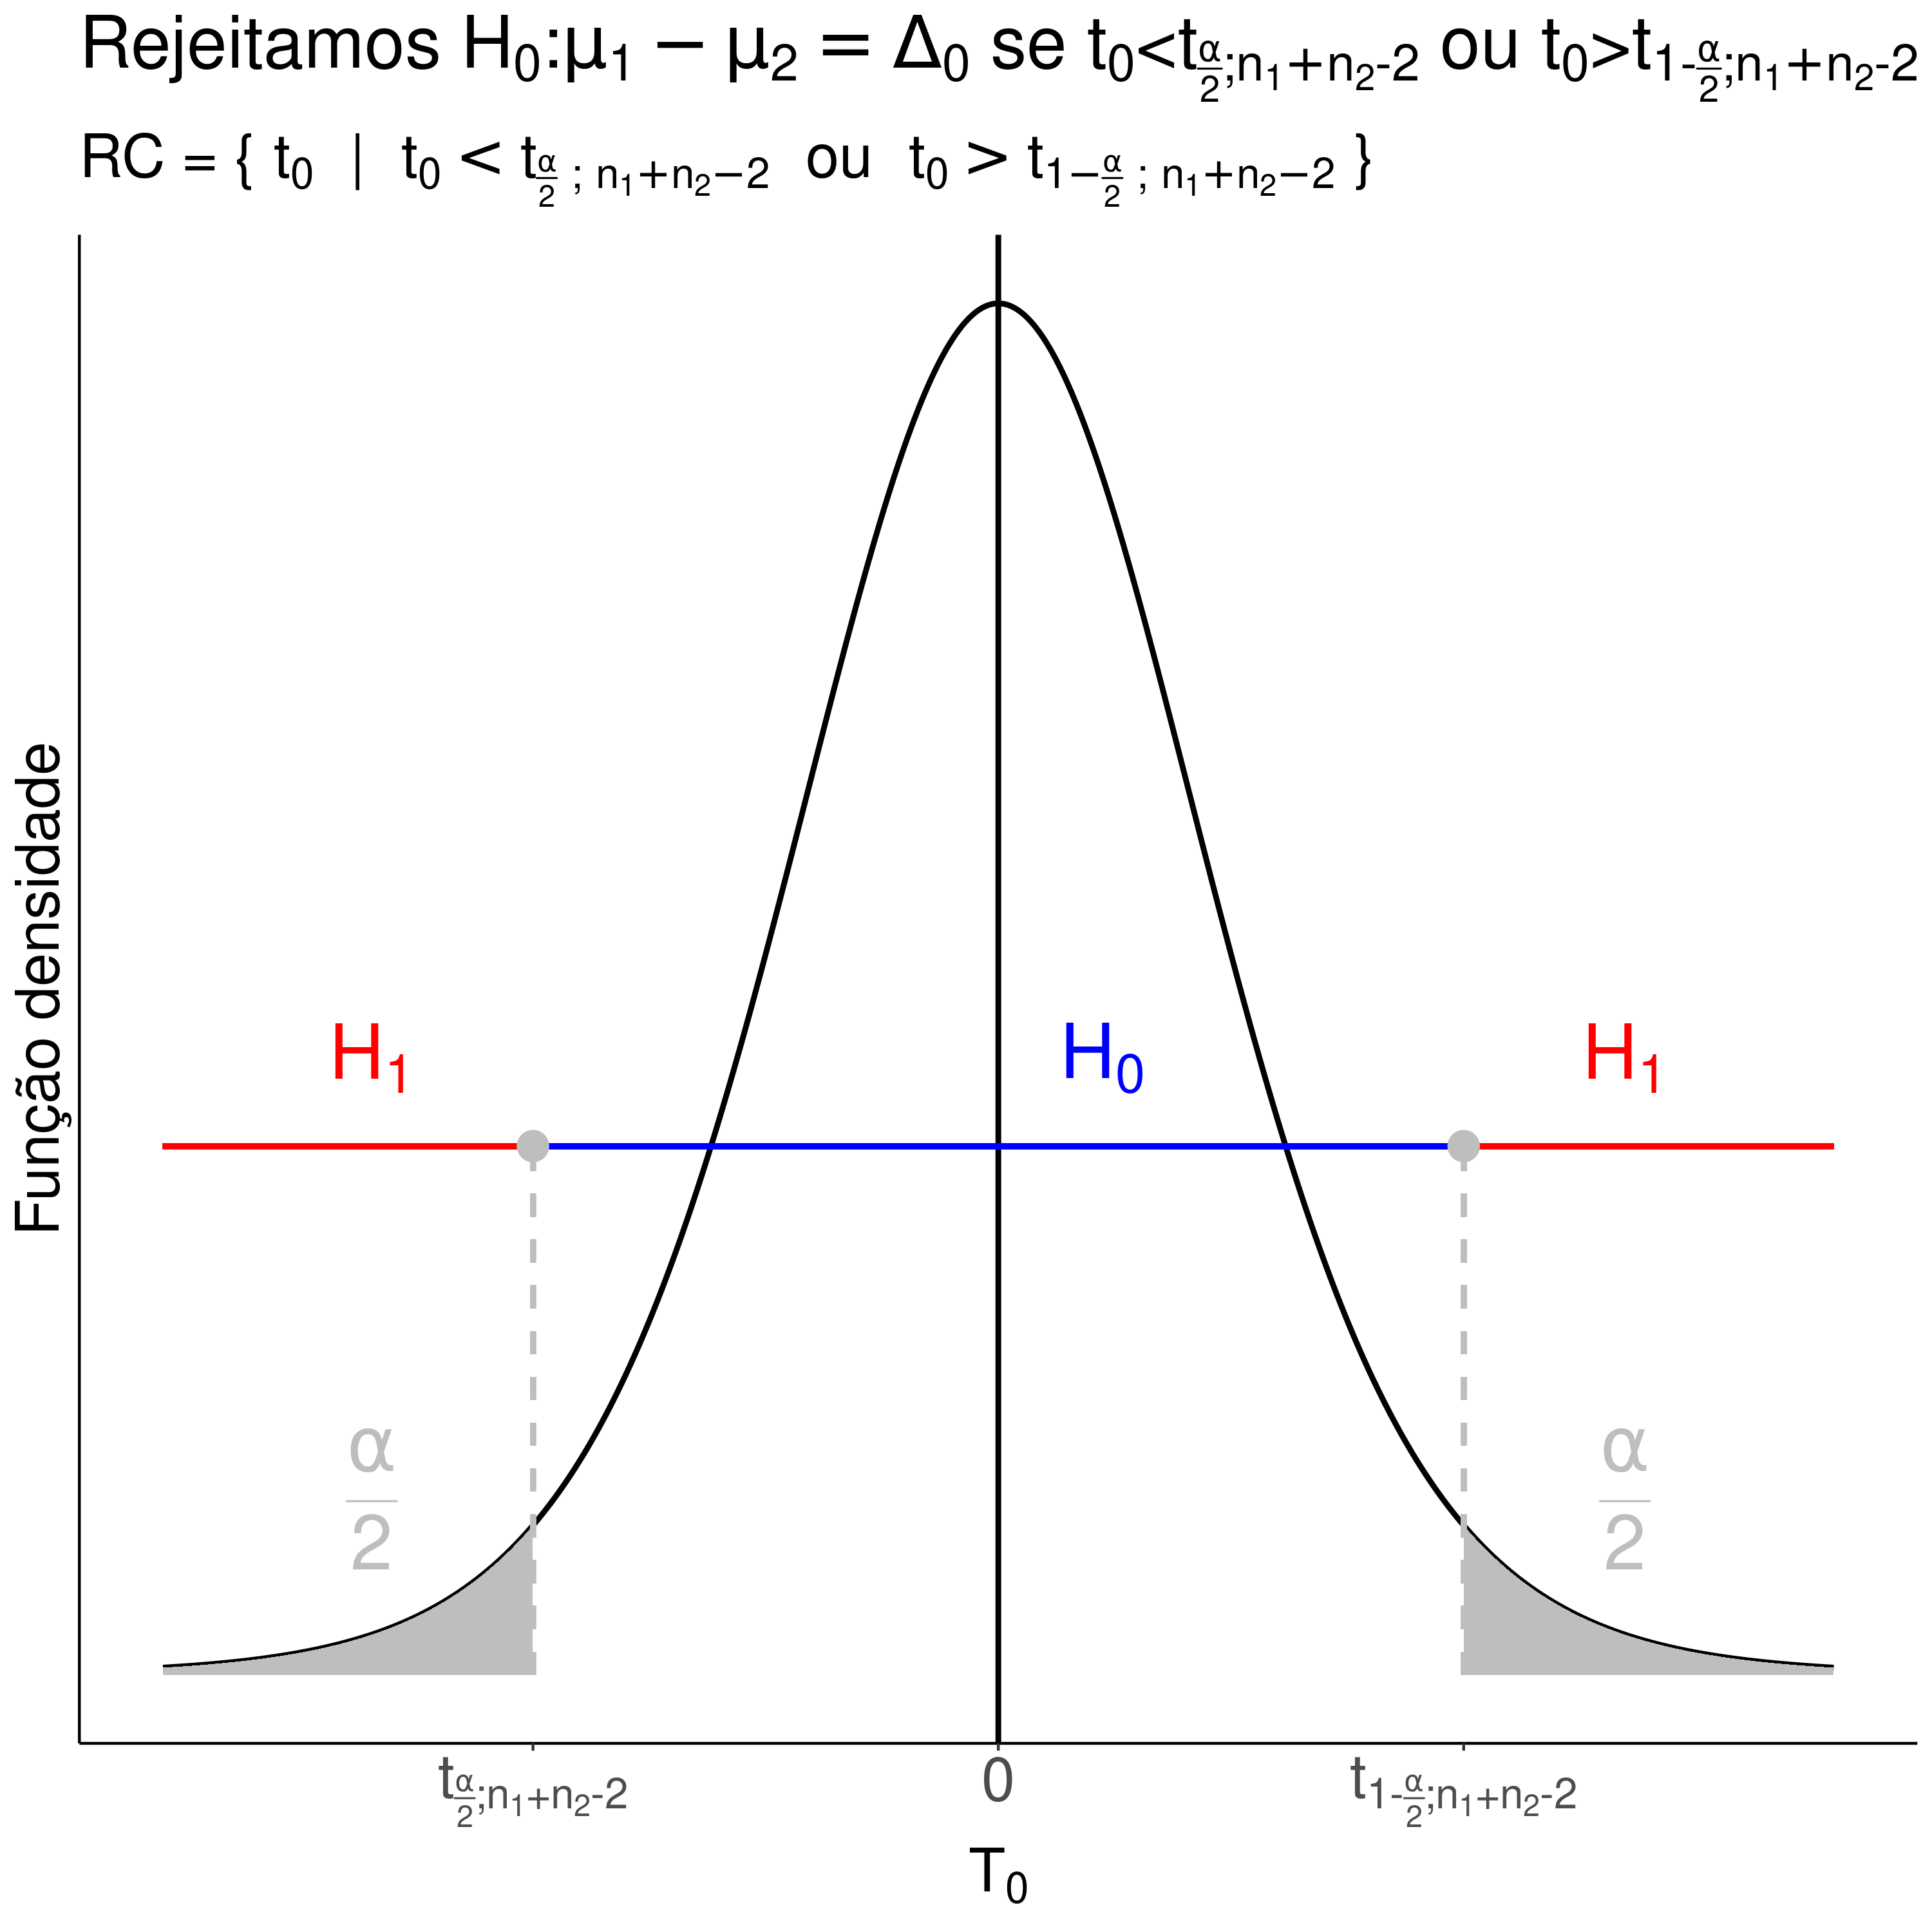
\includegraphics[width=0.32\linewidth]{figures/2-pop-normal-s2-unknown-equal-bilateral.png} \label{fig:2-pop-normal-s2-unknown-equal-bilateral}} \hfill
	\subfloat[][Teste bilateral.]{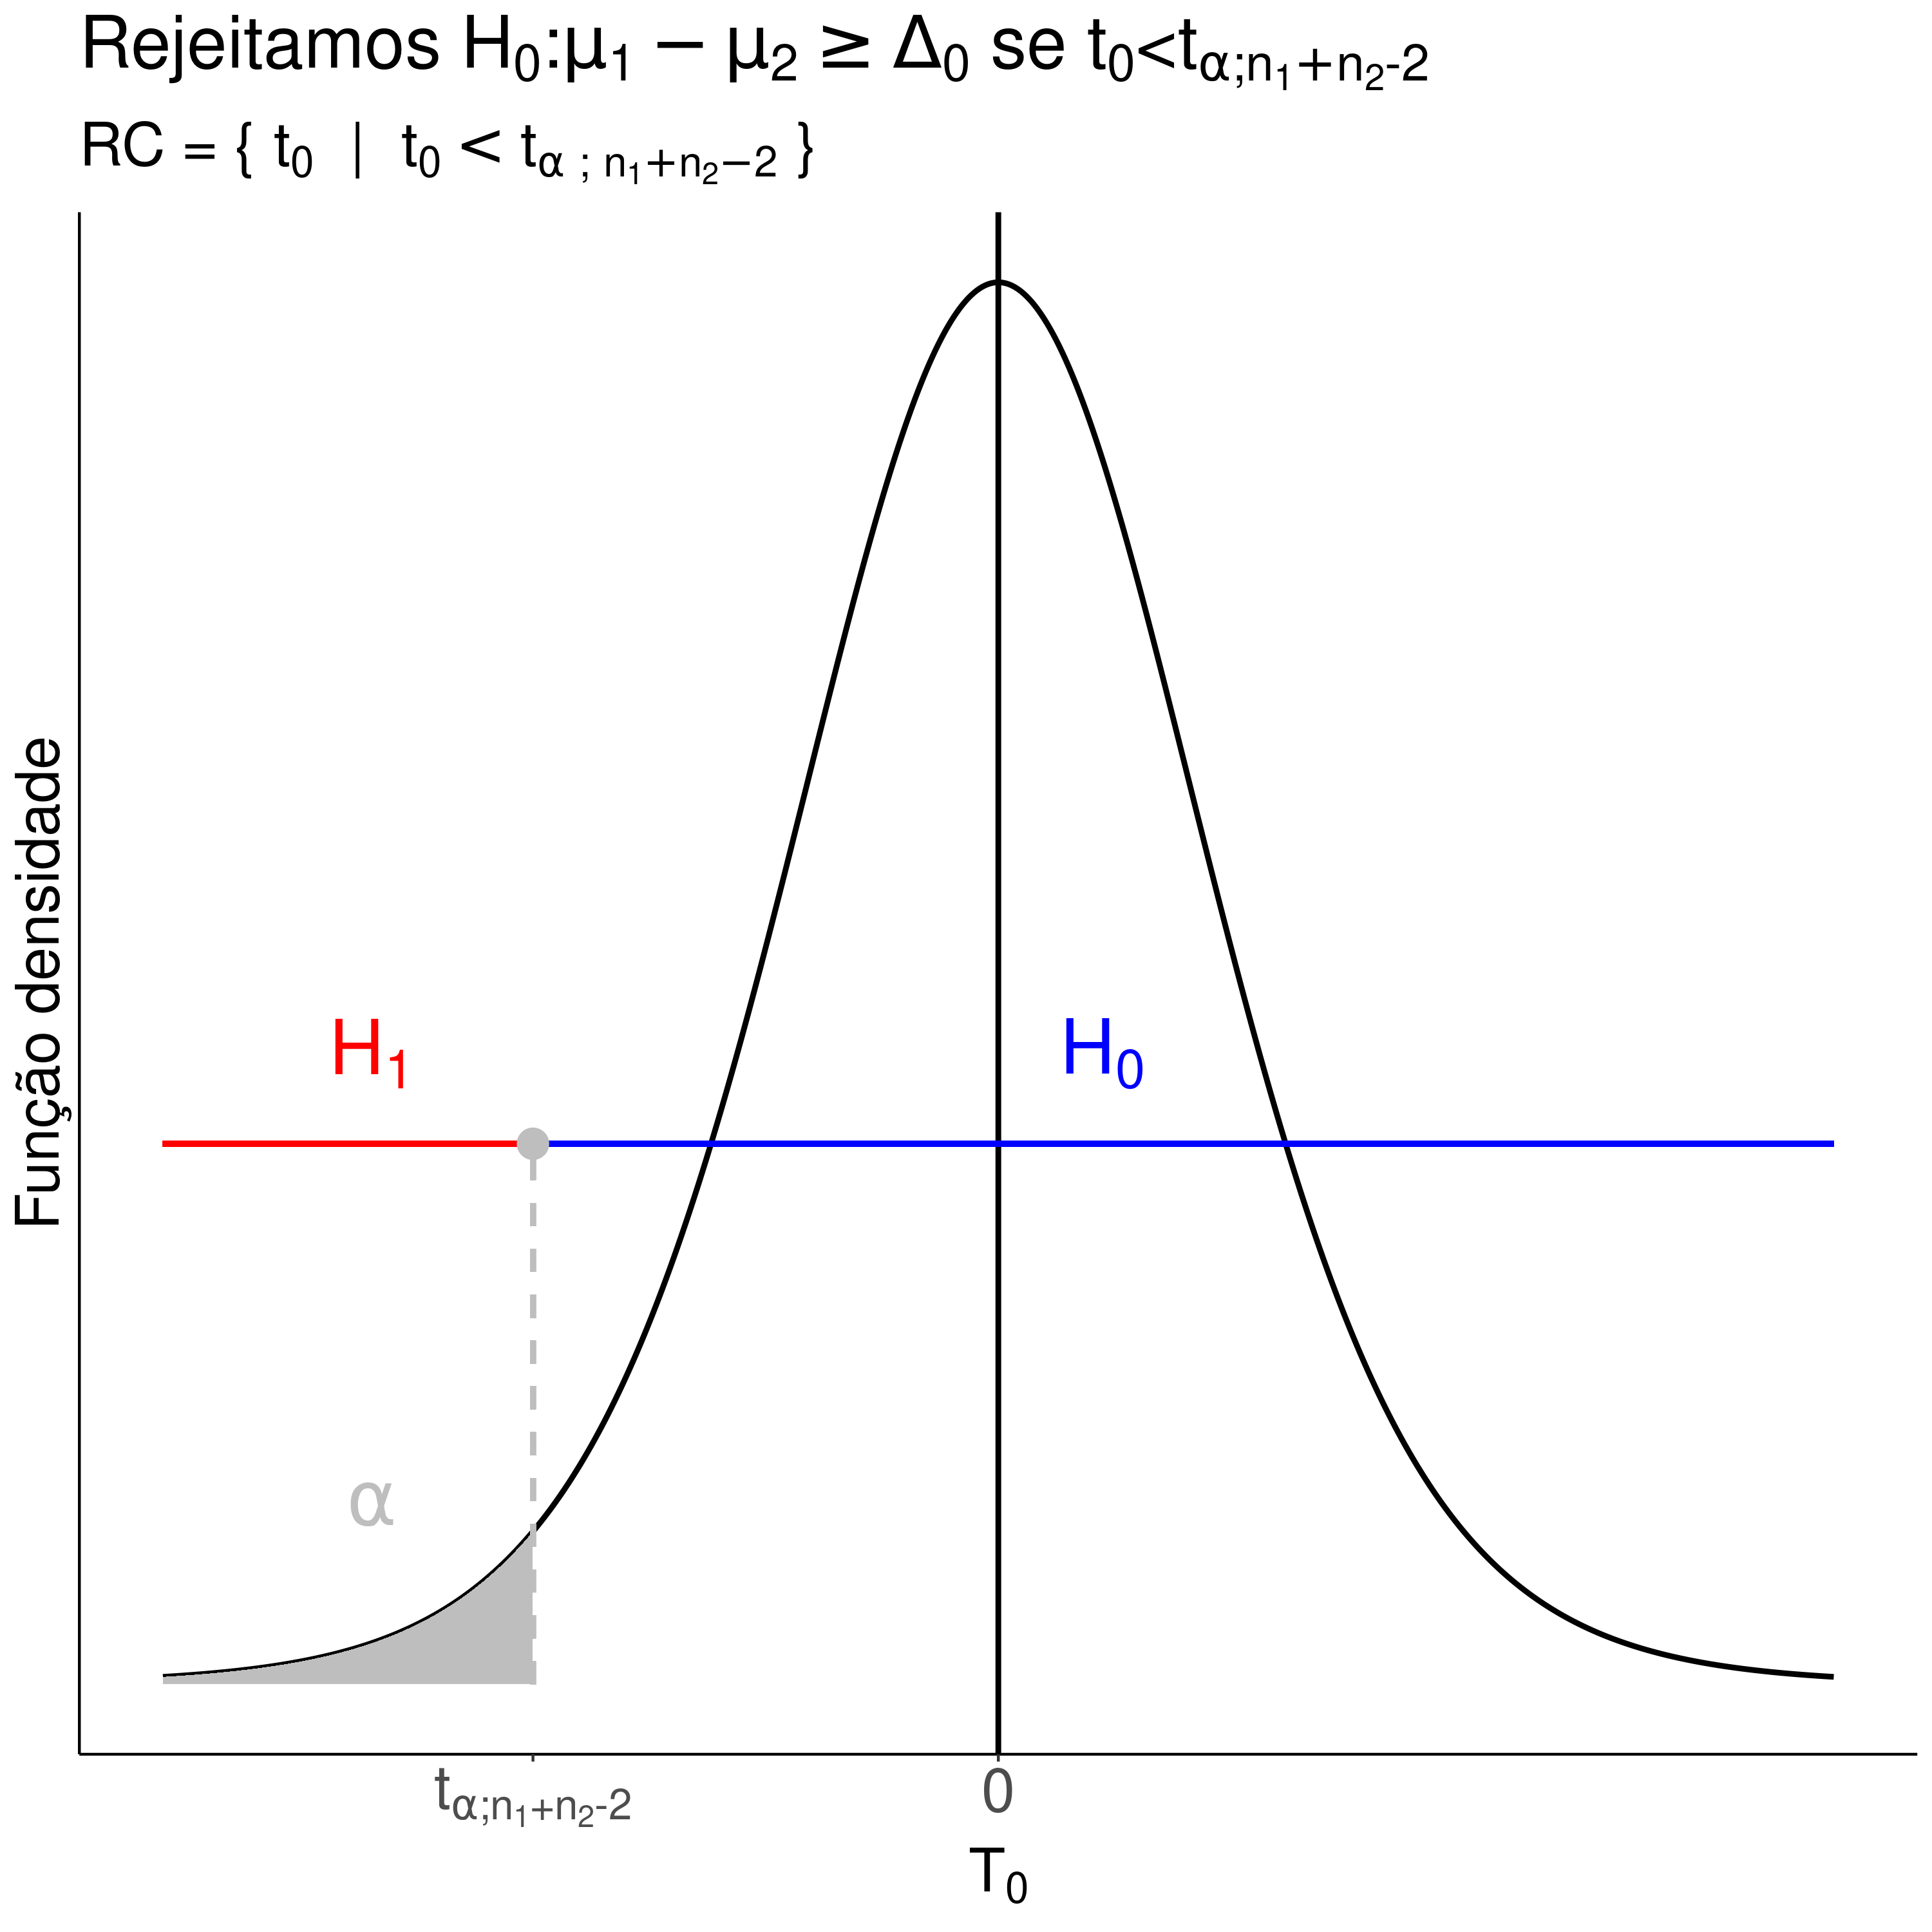
\includegraphics[width=0.32\linewidth]{figures/2-pop-normal-s2-unknown-equal-h1-lower.png} \label{fig:2-pop-normal-s2-unknown-equal-h1-lower}} \hfill
	\subfloat[][Teste bilateral.]{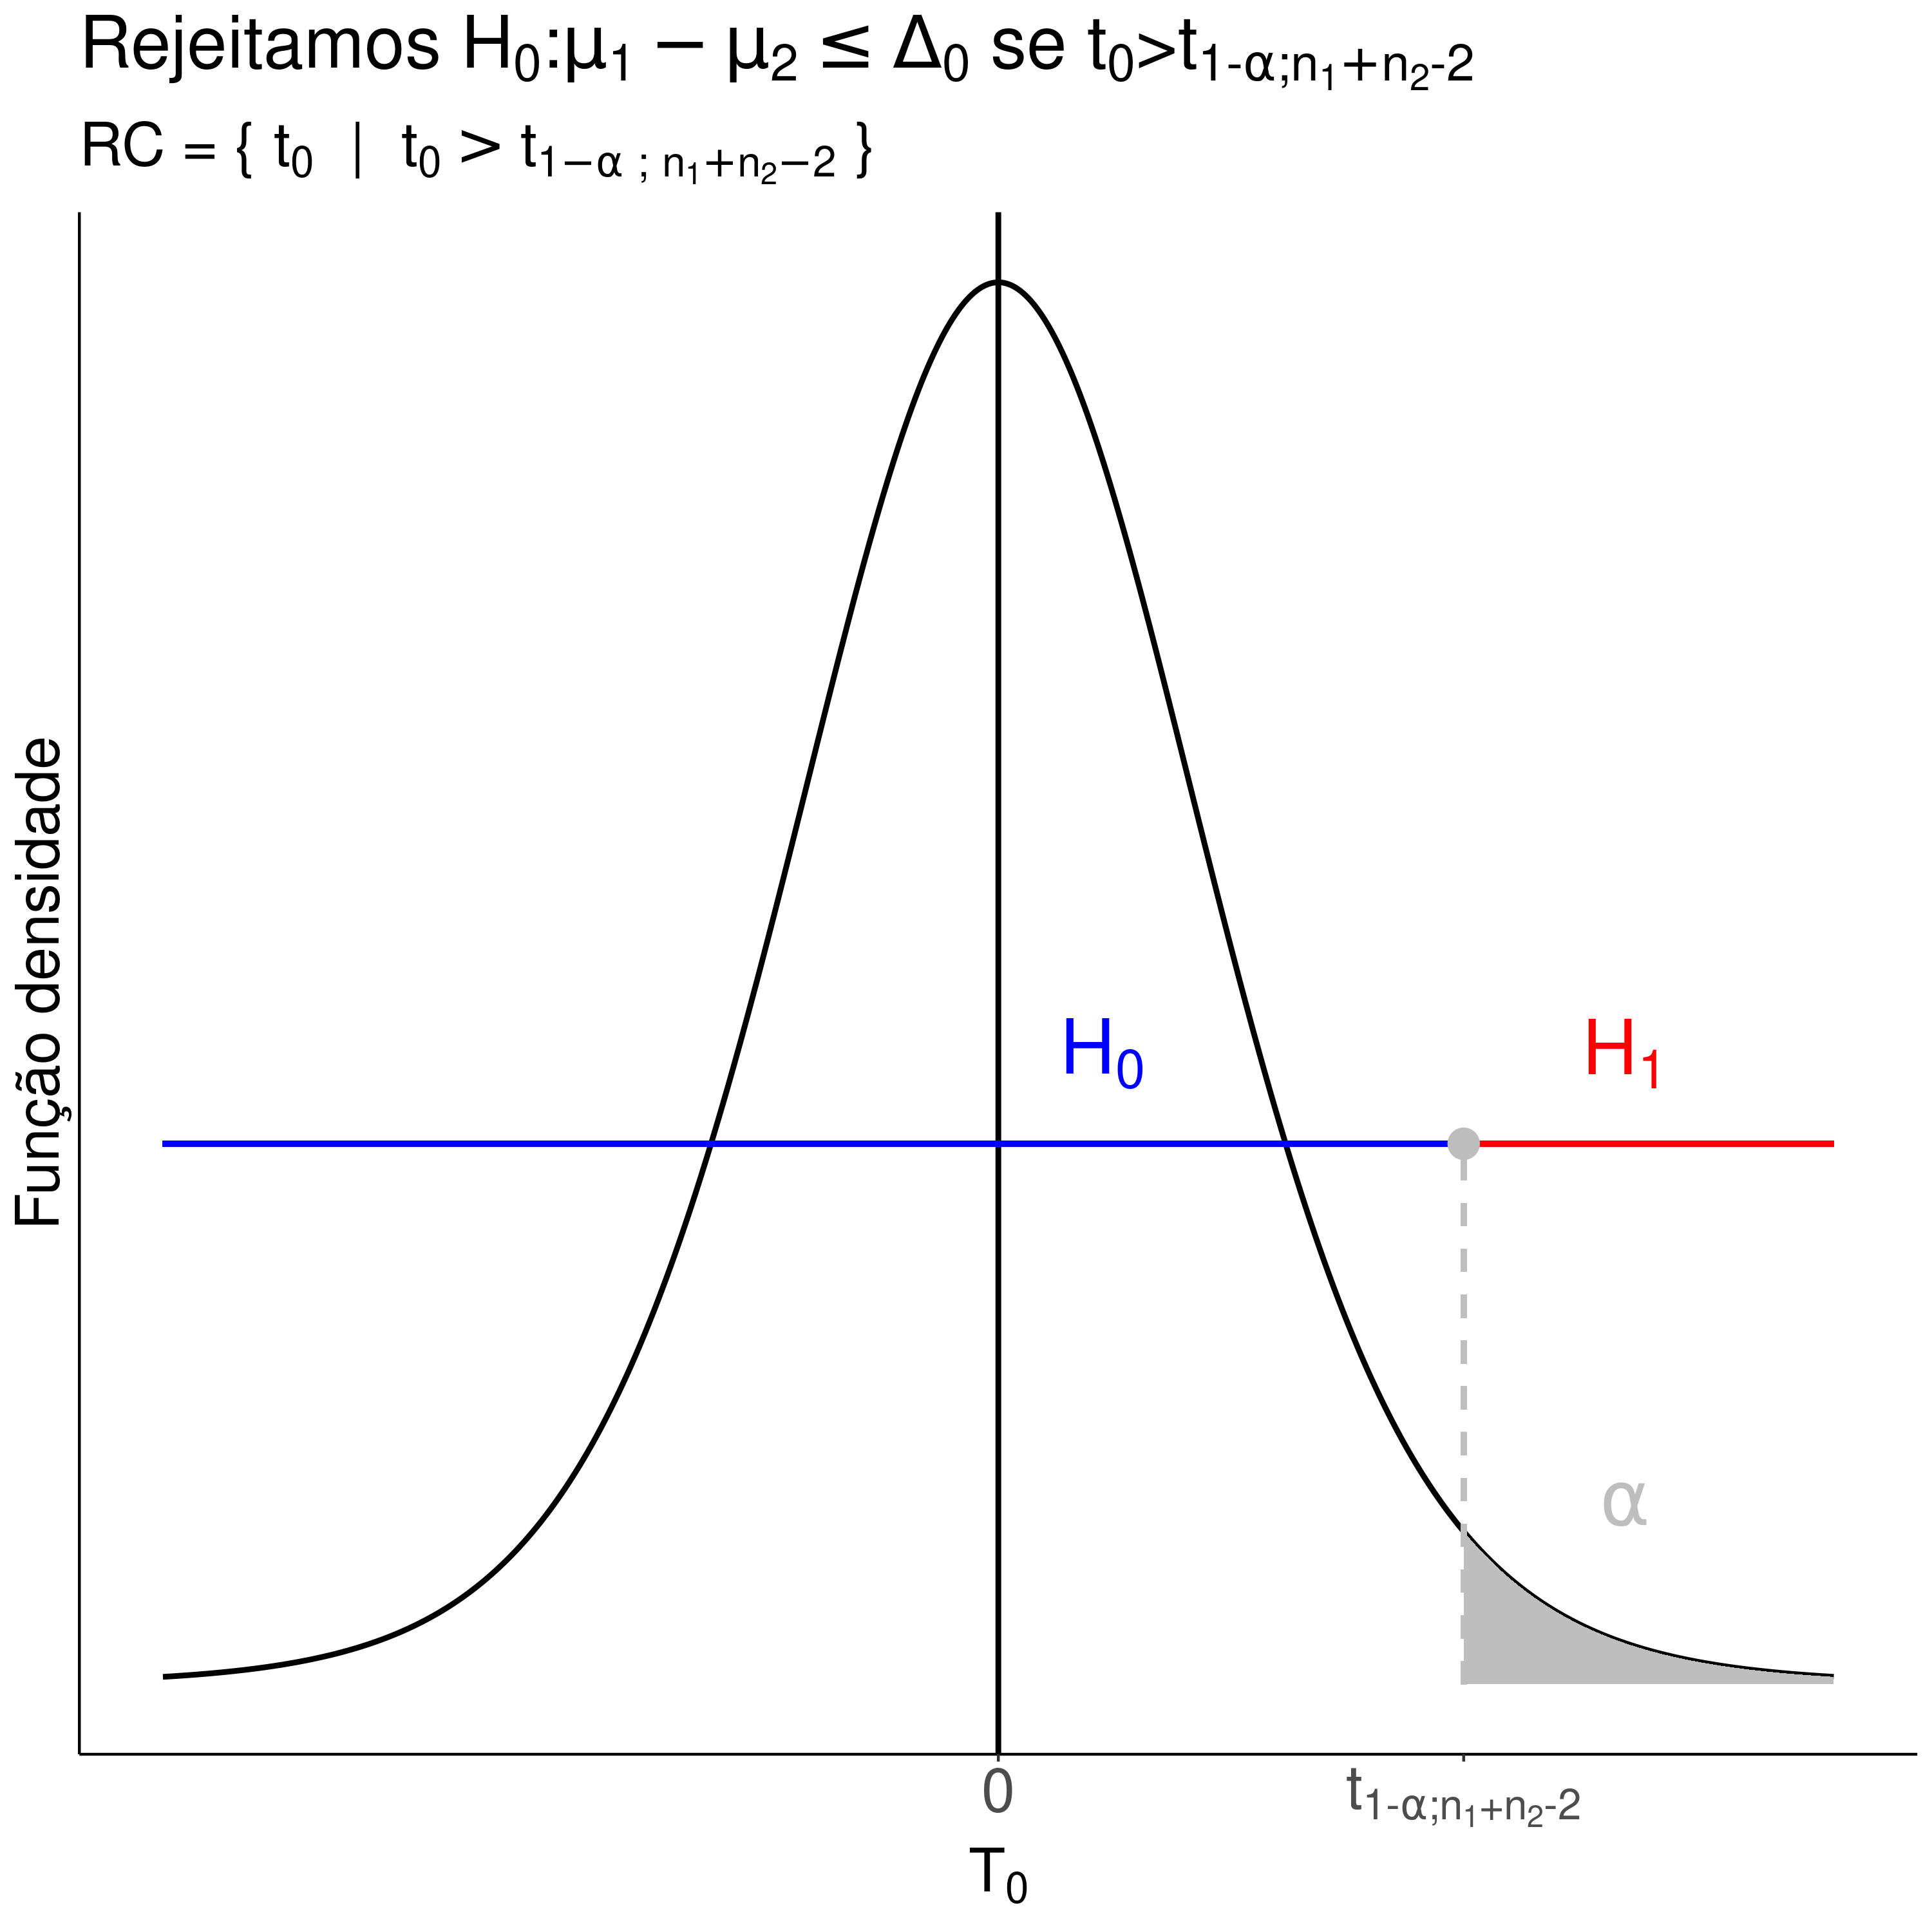
\includegraphics[width=0.32\linewidth]{figures/2-pop-normal-s2-unknown-equal-h1-upper.png} \label{fig:2-pop-normal-s2-unknown-equal-h1-upper}} 
	\caption{Região crítica para comparar médias de populações normais com variâncias desconhecidas e iguais.}
\end{figure}
\end{frame}

\begin{frame}{Comparação de médias $\mu_1$ e $\mu_2$ de duas populações.}

\begin{itemize}
	\item Na Figura~\ref{fig:2-pop-normal-s2-unknown-equal-bilateral}, testamos $H_0: \mu_1 - \mu_2 = \Delta_0$ versus $H_1: \mu_1 - \mu_2 \neq \Delta_0$. Rejeitamos $H_0$ se $t_0 = \frac{\bar{x}_1 - \bar{x}_1 - \Delta_0}{ s_d\sqrt{ \frac{1}{n_1} + \frac{1}{n_2} } } \in  RC=\{t_0 \mid t_0 < t_{\frac{\alpha}{2};n_1+n_2-2} \allowbreak \mbox{ ou } t_0 > t_{1-\frac{\alpha}{2};n_1+n_2-2} \}$, em que $P\left(t_{n_1+n_2-2} \leq t_{\frac{\alpha}{2}; n_1+n_2-2} \right) = \frac{\alpha}{2}$ e $P\left(t_{n_1+n_2-2} \leq t_{1-\frac{\alpha}{2}; n_1+n_2-2} \right) = 1 - \frac{\alpha}{2}$;
	\vfill
	
	\item Na Figura~\ref{fig:2-pop-normal-s2-unknown-equal-h1-lower}, testamos $H_0: \mu_1 - \mu_2 \leq \Delta_0 $ versus $H_1: \mu_1 - \mu_2 > 0$. Rejeitamos $H_0$ se $t_0 = \frac{\bar{x}_1 - \bar{x}_1 - \Delta_0}{ s_d\sqrt{ \frac{1}{n_1} + \frac{1}{n_2} } } \in \allowbreak RC=\{t_0 \mid t_0 > t_{1-\alpha; n_1+n_2-2}  \}$, em que $P\left(t_{n_1+n_2-2} \leq  t_{1-\alpha;n_1+n_2-2} \right) =1- \alpha$;
	\vfill
	
	\item Na Figura~\ref{fig:2-pop-normal-s2-unknown-equal-h1-upper}, testamos $H_0: \mu_1 - \mu_2 \geq \Delta_0$ versus $H_1: \mu_1 - \mu_2  < 0$. Rejeitamos $H_0$ se $t_0 = \frac{\bar{x}_1 - \bar{x}_1 - \Delta_0}{ s_d\sqrt{ \frac{1}{n_1} + \frac{1}{n_2} } } \in \allowbreak RC=\{t_0 \mid t_0 < t_{\alpha;n_1+n_2-2}  \}$, em que $P\left(t_{n_1+n_2-2} \leq t_{\alpha;n_1+n_2-2} \right) = \alpha$.
\end{itemize}
Note que $s_d^2 = \frac{(n_1-1) s_1^2 + (n_2-1) s_2^2}{n_1+n_2-2}$ e chamamos $t_{\alpha;n_1+n_2-2}$, $t_{1-\alpha;n_1+n_2-2}$, $t_{\frac{\alpha}{2};n_1+n_2-2}$ e $t_{1-\frac{\alpha}{2};n_1+n_2-2}$ são chamados de valores críticos.
\end{frame}

\begin{frame}{Comparação de médias $\mu_1$ e $\mu_2$ de duas populações.}

\begin{block}{Exemplo}
	Dois catalisadores estão em análise para determinar como eles afetam o rendimento médio em um processo químico. Especificamente, o catalisador 1 é o padrão do mercado usado pelo processo químico atualmente; o catalisador 2 é um produto novo e mais barato que poderia ser adotado se não alterar o rendimento médio no processo químico. O engenheiro químico responsável pelo processo químico analisou os dois catalisadores e os dados estão na Tabela~\ref{tab:catalisadores}. Assuma a normalidade para rendimento. O rendimento médio dos dois catalisadores são diferentes ao nível de significância $\alpha=5\%$? Calcule o valor-p.
\end{block}

\begin{table}[ht]
	\centering
	\scalebox{0.65}{
	\begin{tabular}{ccc}
		\toprule[0.05cm]
		Número da observação & Catalisador 1 & Catalisador 2 \\ 
		\midrule[0.025cm]
		1 & 91,5 & 89,2 \\ 
		2 & 94,2 & 91,0 \\ 
		3 & 92,2 & 90,5 \\ 
		4 & 95,4 & 93,2 \\ 
		5 & 91,8 & 97,2 \\ 
		6 & 89,1 & 97,0 \\ 
		7 & 94,7 & 91,1 \\ 
		8 & 89,2 & 92,8 \\ 
		\bottomrule[0.05cm]
	\end{tabular}
	}
	\caption{Rendimento para os catalisadores 1 e 2.} 
	\label{tab:catalisadores}
\end{table}

\end{frame}

\begin{frame}{Comparação de médias $\mu_1$ e $\mu_2$ de duas populações.}

Primeiro vamos verificar se as variâncias são iguais.

	\textbf{Passo 1)} Queremos testar as seguintes hipóteses: $H_0: \frac{\sigma_1^2}{\sigma_2^2} = 1$ e $H_1: \frac{\sigma_1^2}{\sigma_2^2} = 1$;
	
	\textbf{Passo 2)} Nível de significância $\alpha=5\%$;
	
	\textbf{Passo 3)} Rejeitamos $H_0$ se $F_0 = \frac{s_1^2}{s_2^2}$ for grande ou for pequeno. Ou seja, $RC = \left\{ f_0 \mid f_0 < f_{\frac{\alpha}{2}; n_1-1, n_2-1} \mbox{ ou } f_{1-\frac{\alpha}{2};n_1-1, n_2-1} < f_0 \right\}$;

	\textbf{Passo 4)} Vamos encontrar os valores críticos:
	\begin{itemize}
		\item $P\left( F_{n_1-1, n_2-1} \leq f_{1-\frac{\alpha}{2};n_1-1, n_2-1} \right) = P\left( F_{n_1-1, n_2-1} \leq f_{0,975;7, 7} \right)$, então $f_{0,975;7, 7} = 4,995$;
		\item $P\left( F_{n_2-1, n_1-1} \leq f_{1-\frac{\alpha}{2};n_2-1, n_1-1} \right) = P\left( F_{n_2-1, n_1-1} \leq f_{0,975;7, 7} \right)$, então $f_{0,975;7, 7} = 4,995$;
		\item $f_{0,025; 7,7} = \frac{1}{ f_{0,975; 7, 7} } = \frac{1}{4,995} = 0,20$.
	\end{itemize}

	\textbf{Passo 5)} Como $s_1 = 2,38$, $s_2 = 2,96$, $n_1=8$, $n_2=8$ e $f_0 = \frac{s_1^2}{s_2^2} = 0,646 \not\in RC$, então não rejeitamos $H_0$ e podemos assumir que os desvios padrões são iguais.
\end{frame}

\begin{frame}{Comparação de médias $\mu_1$ e $\mu_2$ de duas populações.}

\small
\begin{block}{Solução}
	\textbf{Passo 1)} Queremos testar as hipóteses:  $H_0: \mu_1 - \mu_2 = \Delta_0 =0$ e $H_1: \mu_1 - \mu_2 \neq \Delta_0 = 0$;
	
	\textbf{Passo 2)} Nível de significância $\alpha=5\%$;
	
	\textbf{Passo 3)} Rejeito $H_0$ se $\lvert T_0 \rvert = \left\lvert \frac{\bar{X}_1 - \bar{X}_2 - \Delta_0}{S_d \sqrt{\frac{1}{n_1} - \frac{1}{n_2}}} \right\rvert$ for grande. Ou seja, $RC = \left\{ t_0 \mid t_0 < t_{\frac{\alpha}{2}; n_1+n_2-2} \mbox{ ou } t_0 < t_{1-\frac{\alpha}{2}; n_1+n_2-2} \right\}$.
	
	\textbf{Passo 4)} Vamos encontrar os valores críticos:
	\begin{itemize}
		\item $P(t_{n_1+n_2-2} \leq t_{\frac{\alpha}{2}; n_1+n_2-2}) = P(t_{14} \leq t_{0,025; 14}) = \frac{\alpha}{2} = 0,025$, então $t_{0,025; 14} = -2,145$;
		\item $P(t_{n_1+n_2-2} \leq t_{1-\frac{\alpha}{2}; n_1+n_2-2}) = P(t_{14} \leq t_{0,975; 14}) = \frac{\alpha}{2} = 0,975$, então $t_{0,975; 14} = 2,145$.
	\end{itemize}

	\textbf{Passo 5)} Observe que $\bar{x}_1=92,25$, $\bar{x}_2 = 92,73$, $s_1=2,39$, $s_2=2,98$, $n_1=n_2=8$, $s_d^2=2,7$ $\Delta_0=0$, $t_0=-0,36$, então $t_0 \not\in RC$ e não temos evidência para rejeitar $H_0$.
	
	Ou seja, ao nível de significância de $\alpha=5\%$, não encontramos diferença no rendimento médio entre os dois catalisadores e o engenheiro químico deveria recomendar o uso do catalisador 2 que é mais barato.
\end{block}
\normalsize
\end{frame}

\begin{frame}{Comparação de médias $\mu_1$ e $\mu_2$ de duas populações.}

\begin{block}{Solução (valor-p)}
	Como encontrar o valor-p
	$$p=P(\lvert T_0 \rvert > \lvert t_0 \rvert  \mid H_0) = 2 \cdot(1- P(t_{n_1+n_2-2} \leq \lvert t_0 \rvert)).$$
	
	 Como $\bar{x}_1=92,25$, $\bar{x}_2 = 92,73$, $s_1=2,39$, $s_2=2,98$, $n_1=n_2=8$, $s_d^2=2,7$ $\Delta_0=0$, $t_0=-0,36$, então
	 \begin{align*}
		 p &= 2 \cdot [1 - P(t_{n_1+n_2-2} \leq \lvert t_0 \rvert)]\\
		 &= 2 \cdot [1 - P(t_{22} \leq \lvert -0,36 \rvert)]\\
		 &= 2 \cdot [1 - 0,6389]\\
		 &= 0,7223.
	 \end{align*}
	 
	 Como $p=0,7223 > \alpha = 0,05$, não rejeitamos $H_0$ ao nível de significância $\alpha=5\%$, ou seja, o rendimento médio no processo químico para os dois catalisadores são equivalentes.
\end{block}

\end{frame}

\begin{frame}{Comparação de médias $\mu_1$ e $\mu_2$ de duas populações.}
	\begin{block}{Exemplo}
			Um pesquisador está analisando rebolos abrasivos. Os dados sobre a força de moagem com os rebolos abrasivos (em $N$) para dois níveis de vibração, baixa e alta, estão na Tabela~\ref{tab:moagem}. Assuma que a força de moagem tem distribuição normal. Existe evidência que vibração mais alta produz uma força de moagem maior ao nível de significância $\alpha=5\%$? Calcule o valor-p.
			\begin{table}[ht]
				\centering
				\scalebox{0.6}{
				\begin{tabular}{cc}
					\toprule[0.05cm]
					Vibração baixa & Vibração alta \\ 
					\midrule[0.025cm]
						224 & 327 \\ 
						268 & 352 \\ 
						293 & 379 \\ 
						190 & 347 \\ 
						273 & 335 \\ 
						275 & 323 \\ 
						243 & 325 \\ 
						244 & 422 \\ 
						243 & 354 \\ 
						233 & 335 \\ 
						246 & 337 \\ 
						230 & 364 \\ 
					\bottomrule[0.05cm]
				\end{tabular}
				}
				\caption{Força de moagem para níveis baixos e altos de vibração.} 
				\label{tab:moagem}
			\end{table}
	\end{block}
\end{frame}

\begin{frame}{Comparação de médias $\mu_1$ e $\mu_2$ de duas populações.}

\small
\begin{block}{Solução}

	Primeiro verificamos as variâncias da força de moagem são iguais.
	
	\textbf{Passo 1)} Queremos testar as hipóteses: $H_0: \frac{\sigma_1^2}{\sigma_2^2} = 1$ e $H_1: \frac{\sigma_1^2}{\sigma_2^2} \neq 1$;
	
	\textbf{Passo 2)} Nível de significância $\alpha=5\%$;
	
	\textbf{Passo 3)} Rejeitamos $H_0$ se $F_0 = \frac{S_1^2}{S_2^2}$ for grande ou for pequeno. Ou seja, $RC = \left\{ f_0 \mid f_0 < f_{\frac{\alpha}{2}; n_1-1, n_2-1} \mbox{ ou } f_{1-\frac{\alpha}{2}; n_1-1, n_2-1} < f_0 \right\}$;
	
	\textbf{Passo 4)} Vamos encontrar os valores críticos:
	\begin{itemize}
		\item $P\left( F_{n_1-, n_2-1}  \leq f_{1-\frac{\alpha}{2}; n_1-1, n_2-1} \right) =  P\left( F_{11, 11}  \leq f_{0,975; 11, 11} \right) = 1 - \frac{\alpha}{2} = 0,975$, então $f_{0,975; 11, 11} = 3,474$;
		\item $P\left( F_{n_2-, n_1-1}  \leq f_{1-\frac{\alpha}{2}; n_2-1, n_1-1} \right) =  P\left( F_{11, 11}  \leq f_{0,975; 11, 11} \right) = 1 - \frac{\alpha}{2} = 0,975$, então $f_{0,975; 11, 11} = 3,474$;
		\item $f_{\frac{\alpha}{2}; n_1-1, n_2-1} = \frac{1}{f_{1-\frac{\alpha}{2}; n_2-1, n_1-1}}=\frac{1}{3,474} = 0,2879$.
	\end{itemize}	

	\textbf{Passo 5)} Como $n_1=n_2=12$, $s_1 = 27,50$, $s_2 = 28,21$ e $f_0 = \frac{s_1^2}{s_2^2} = 0,951 \not\in RC$, então não rejeitamos $H_0$ e decidimos que as duas variâncias são iguais.
\end{block}
\normalsize

\end{frame}

\begin{frame}{Comparação de médias $\mu_1$ e $\mu_2$ de duas populações.}


\begin{block}{Solução}
	\textbf{Passo 1)} Seja $\mu_1$ a média de força de moagem usando vibração baixa e $\mu_2$ a média de força de moagem usando vibração alta. Então, queremos testar as seguintes hipóteses: $H_0: \mu_1 - \mu_2 \geq \Delta_0 = 0$ e $H_1: \mu_1 - \mu_2 < \Delta_0=0$;
	
	\textbf{Passo 2)} Nível de significância $\alpha=5\%$;
	
	\textbf{Passo 3)} Rejeito $H_0$ se $T_0 = \frac{\bar{X}_1 - \bar{X}_2 - \Delta_0}{S_d\sqrt{\frac{1}{n_1} + \frac{1}{n_2}}}$ for pequeno. Ou seja, $RC=\left\{ t_0 \mid t_0 < t_{\alpha;n_1+n_2-2} \right\}$;
	
	\textbf{Passo 4)} Vamos encontrar os valores críticos:
	\begin{itemize}
		\item $P(t_{n_1+n_2-2} \leq t_{\alpha; n_1+n_2-2}) = P(t_{22} \leq t_{0,05; 22}) = \alpha = 0,05$, então $t_{0,05; 22} = - 1,717$.
	\end{itemize}

	\textbf{Passo 5)} Como $\Delta_0 = 0$, $\bar{x}_1 = 246,83$, $\bar{x}_2 = 350$, $s_1 = 27,50$, $s_2 = 28, 21$, $t_0 = -9,07$, então $t_0 \in RC$ e rejeitamos $H_0$. Ou seja, a força de moagem é maior para vibração mais alta.
\end{block}


\end{frame}

\begin{frame}{Comparação de médias $\mu_1$ e $\mu_2$ de duas populações.}

\begin{block}{Solução (valor-p)}
	O valor-p é calculado por
	$$p = P(T_0 < t_0 \mid H_0) = P(t_{n_1+n_2-2} \leq t_0).$$
	
	 Como $\Delta_0 = 0$, $\bar{x}_1 = 246,83$, $\bar{x}_2 = 350,27$, $s_1 = 28,21$, $s_2 = 27,86$, $n_1=n_2=12$, $t_0 = -9,07$, então
	 \begin{align*}
		 p &= P (t_{n_1+n_2-2} \leq t_0)\\
		 &= P(t_{22} \leq -9,07)\\
		 &= 0.	 
	 \end{align*}
	 
	 Como $p=0 < \alpha = 0,05$, então rejeitamos $H_0$ ao nível de significância $\alpha=5\%$, ou seja, a força de moagem é maior para a vibração mais alta ao nível de significância $\alpha=5\%$.
\end{block}

\end{frame}

\subsection{Poder e tamanho da amostra.}

\begin{frame}{Poder do teste: $H_0:\mu_1 - \mu_2 = \Delta_0$ e $H_1: \mu_1 - \mu_2 \neq \Delta_0$.}

\tiny

Imagine que
\begin{itemize}
	\item Hipóteses: $H_0: \mu_1 - \mu_2 = \Delta_0$ e $H_1: \mu_1 -  \mu_2 \neq \Delta_0$;
	\item $H_1$ é verdade, então $\Delta = \mu_1-\mu_2 \neq \Delta_0$;
	\item As variâncias $\sigma_1^2$  e $\sigma_2^2$ das duas populações são iguais e desconhecidas. Usamos $S_d^2 = \frac{(n_1-1)s_1^2 + (n_2-1)s_2^2}{n_1+n_2-2}$;
	\item $T_0 = \frac{\bar{X}_1 - \bar{X}_2 - \Delta_0}{ S_d \sqrt{ \frac{1}{n_1} + \frac{1}{n_2} } } \sim t_{n_1+n_2-2}\left( \frac{\mu_1 - \mu_2 - \Delta_0}{\sigma \sqrt{\frac{1}{n_1} + \frac{1}{n_2}}} \right)$. Chamamos $d = \frac{\mu_1-\mu_2-\Delta_0}{\sigma}$ de tamanho do efeito;
	\item Ao nível de significância $\alpha$, temos $RC = \{ t_0 \mid t_0 < t_{\frac{\alpha}{2};n_1+n_2-2} \mbox{ ou } t_{1-\frac{\alpha}{2};n_1+n_2-2} < t_0  \}$.
\end{itemize}
\vfill	

Poder do teste é dado
\begin{align*}
\textcolor{important}{1-\beta} &=1 - \left[P\left( t_{\frac{\alpha}{2};n_1+n_2-2} \leq T_0 \leq t_{1-\frac{\alpha}{2};n_1+n_2-2} \mid H_1 \right)\right]\\
&= 1 - \left[P\left( t_{\frac{\alpha}{2};n_1+n_2-2} \leq T_0 \leq t_{1-\frac{\alpha}{2};n_1+n_2-2} \mid \Delta \neq \Delta_0 \right)\right]\\
&= \textcolor{important}{1 - P\left( t_{n_1+n_2-2}\left( \frac{\mu_1 - \mu_2 - \Delta_0}{\sigma \sqrt{\frac{1}{n_1} + \frac{1}{n_2}}} \right) \leq t_{1-\frac{\alpha}{2};n_1+n_2-2} \right) + P\left( t_{n_1+n_2-2}\left( \frac{\mu_1 - \mu_2 - \Delta_0}{\sigma \sqrt{\frac{1}{n_1} + \frac{1}{n_2}}} \right) \leq t_{\frac{\alpha}{2};n_1+n_2-2} \right).}
\end{align*}
\vfill

A \textcolor{important}{Função Poder}, dado o tamanho da amostra $n$, é uma função das médias populacionais na hipótese alternativa  $\pi: \mathbb{R} - \{\Delta_0\} \longrightarrow [0,1]$ dada por
\begin{align*}
\pi(\delta) = 1 - P\left( t_{n_1+n_2-2}\left( \frac{\mu_1 - \mu_2 - \Delta_0}{\sigma \sqrt{\frac{1}{n_1} + \frac{1}{n_2}}} \right) \leq t_{1-\frac{\alpha}{2};n_1+n_2-2} \right) + P\left( t_{n_1+n_2-2}\left( \frac{\mu_1 - \mu_2 - \Delta_0}{\sigma \sqrt{\frac{1}{n_1} + \frac{1}{n_2}}} \right) \leq t_{\frac{\alpha}{2};n_1+n_2-2} \right),
\end{align*}
em que $\Delta = \mu_1 - \mu_2, \Delta \in \mathbb{R} - \{\Delta_0 \}$. Alguns livros chamam a Função Poder de \textcolor{important}{Curva de Característica Operacional.}

\normalsize

\end{frame}


\begin{frame}[fragile]{Tamanho da amostra: $H_0:\mu_1 - \mu_2 = \Delta_0$ e $H_1: \mu_1 - \mu_2 \neq \Delta_0$.}

\tiny

Imagine que
\begin{itemize}
	\item Hipóteses: $H_0: \mu_1 - \mu_2 = \Delta_0$ e $H_1: \mu_1 -  \mu_2 \neq \Delta_0$;
	\item $H_1$ é verdade, então $\Delta = \mu_1-\mu_2 \neq \Delta_0$;
	\item As variâncias $\sigma_1^2$  e $\sigma_2^2$ das duas populações são iguais e desconhecidas. Usamos $S_d^2 = \frac{(n_1-1)s_1^2 + (n_2-1)s_2^2}{n_1+n_2-2}$;
	\item $T_0 = \frac{\bar{X}_1 - \bar{X}_2 - \Delta_0}{ S_d \sqrt{ \frac{1}{n_1} + \frac{1}{n_2} } } \sim t_{n_1+n_2-2}\left( \frac{\mu_1 - \mu_2 - \Delta_0}{\sigma \sqrt{\frac{1}{n_1} + \frac{1}{n_2}}} \right)$, em que $\frac{\mu_1 - \mu_2 - \Delta_0}{\sigma \sqrt{\frac{1}{n_1} + \frac{1}{n_2}}}$ é o parâmetro de não-centralidade da distribuição t-Student;
	\item Ao nível de significância $\alpha$, temos $RC = \{ t_0 \mid t_0 < t_{\frac{\alpha}{2};n_1+n_2-2} \mbox{ ou } t_{1-\frac{\alpha}{2};n_1+n_2-2} < t_0  \}$.
\end{itemize}
\vfill

Considere $1-\beta$, $\alpha$ $n_1=n_2=n$, então o tamanho \sout{mínimo} da amostra é solução da seguinte equação
\begin{align} \label{eq:pwr-t-test-2pop-bilateral}
1-\beta = 1 - P\left( t_{2n-2}\left( \frac{\mu_1 - \mu_2 - \Delta_0}{\sigma \sqrt{\frac{2}{n}}} \right) \leq t_{1-\frac{\alpha}{2};2n-2} \right) + P\left( t_{2n-2}\left( \frac{\mu_1 - \mu_2 - \Delta_0}{\sigma \sqrt{\frac{2}{n}}} \right) \leq t_{\frac{\alpha}{2};2n-2} \right).
\end{align}

A equação~\eqref{eq:pwr-t-test-2pop-bilateral} é resolvida usando métodos numéricos que estão implementados em diversos \textit{softwares}.
\begin{description}
	\item[No R] \lstinline|pwr_sigma_2pop|
\end{description}
Esta função está no pacote \lstinline|power|, que pode ser instalado usando o pacote \lstinline|devtools|: \lstinline|devtools::install_github("gilberto-sassi/power")|.

\normalsize
\end{frame}

\begin{frame}{Poder do teste: $H_0:\mu_1 - \mu_2 = \Delta_0$ e $H_1: \mu_1 - \mu_2 \neq \Delta_0$.}

\begin{block}{Exemplo}
	Dois catalisadores estão em análise para determinar como eles afetam o rendimento médio em um processo químico. Especificamente, o catalisador 1 é o padrão do mercado usado pelo processo químico atualmente; o catalisador 2 é um produto novo e mais barato que poderia ser adotado se não alterar o rendimento médio no processo químico. O engenheiro químico responsável pelo processo químico planeja analisar os dois catalisadores com uma amostra de oito observações para cada catalisador. Assuma a normalidade, com o mesmo desvio padrão $\sigma=3$, para rendimento. Em estudo piloto, o engenheiro químico descobriu que as médias população são $\mu_1 = 92$ e $\mu_2 = 93$.  Qual o poder do teste para checar se o rendimento dos dois catalisadores são iguais? Use $\alpha=5\%$. 
\end{block}

\end{frame}

\begin{frame}[fragile]{Poder do teste: $H_0:\mu_1 - \mu_2 = \Delta_0$ e $H_1: \mu_1 - \mu_2 \neq \Delta_0$.}

\scriptsize
\begin{block}{Solução}
	\textbf{Passo 1)} Queremos testar as hipóteses: $H_0: \mu_1 - \mu_2 = \Delta_0=0$ e $H_1: \mu_1  - \mu_2 \neq \Delta_0=0$;
	
	\textbf{Passo 2)} Nível de significância $\alpha=5\%$;
	
	Como $\sigma=3$, $n_1=n_2=8$, $\Delta_0 = 0$, $\mu_1=92$, $\mu_2=93$, então o parâmetro de não-centralidade $\mu = \frac{\mu_1 - \mu_2 - \Delta_0}{\sigma \sqrt{\frac{1}{n_1} + \frac{1}{n_2}}}=\frac{92-93 - 0}{3\sqrt{\frac{1}{8} + \frac{1}{8}}} = -0,67$.
		
	Vamos encontrar os quantis da distribuição $t$-Student:
	\begin{itemize}
		\item $P(t_{n_1+n_2-2} \leq t_{\frac{\alpha}{2}; n_1+n_2-2}) = P(t_{14} \leq t_{0,025; 14}) = \frac{\alpha}{2} = 0,025$, então $t_{0,025; 14} = -2,145$;
		\item $P(t_{n_1+n_2-2} \leq t_{1-\frac{\alpha}{2}; n_1+n_2-2}) = P(t_{14} \leq t_{0,975; 14}) =1- \frac{\alpha}{2} = 0,975$, então $t_{0,975; 14} = 2,145$.
	\end{itemize}

	Então, o poder do teste é dado por
	\begin{align*}
		1-\beta &= 1 - P\left( t_{n_1+n_2-2}\left(\mu\right) \leq t_{1-\frac{\alpha}{2};n_1+n_2-2} \right) + P\left( t_{n_1+n_2-2}\left(\mu \right) \leq t_{\frac{\alpha}{2};n_1+n_2-2} \right)\\
		&= 1 - P\left(t_{14}(-0,67) \leq 2,145\right) + P\left(t_{14}(-0,67) \leq -2,145\right) = 0,096.
	\end{align*}
\end{block}

\begin{lstlisting}[language = C, caption = Código no R.]
pwr_t_test_2pop_homo(sigma = 3, delta= 92 - 93, delta0 = 0, n1 = 8,
			n2 = 8, pwr = NULL, alternative = "two.sided", sig_level = 0.05)
\end{lstlisting}

\normalsize

\end{frame}

\begin{frame}{Tamanho da amostra: $H_0:\mu_1 - \mu_2 = \Delta_0$ e $H_1: \mu_1 - \mu_2 \neq \Delta_0$.}

\begin{block}{Exemplo}
	Dois catalisadores estão em análise para determinar como eles afetam o rendimento médio em um processo químico. Especificamente, o catalisador 1 é o padrão do mercado usado pelo processo químico atualmente; o catalisador 2 é um produto novo e mais barato que poderia ser adotado se não alterar o rendimento médio no processo químico. O engenheiro químico responsável pelo processo químico planeja analisar os dois catalisadores. Assuma a normalidade, com o mesmo desvio padrão $\sigma=3$, para rendimento. Em estudo piloto, o engenheiro químico descobriu que as médias população são $\mu_1 = 92$ e $\mu_2 = 93$.  Quantas observações de rendimento de cada catalisador precisamos coletar para termos um poder de teste de $99\%$? Use $\alpha=5\%$. 
\end{block}

\end{frame}

\begin{frame}[fragile]{Tamanho da amostra: $H_0:\mu_1 - \mu_2 = \Delta_0$ e $H_1: \mu_1 - \mu_2 \neq \Delta_0$.}

\small
\begin{block}{Solução}
	\textbf{Passo 1)} Queremos testar as hipóteses: $H_0: \mu_1 - \mu_2 = \Delta_0=0$ e $H_1: \mu_1  - \mu_2 \neq \Delta_0=0$;
	
	\textbf{Passo 2)} Nível de significância $\alpha=5\%$;
		
	Como $\sigma=3$, $\alpha = 0,05$, $\mu_1=92$, $\mu=93$, $\Delta_0=0$ e $1-\beta=99\%$. Assuma que $n_1=n_2=n$, então o tamanho \sout{mínimo} da amostra é solução da seguinte equação
	\scriptsize
	\begin{align*}
		1-\beta &= 0,99 =  1 - P\left( t_{2n-2}\left( \frac{\mu_1 - \mu_2 - \Delta_0}{\sigma \sqrt{\frac{2}{n}}} \right) \leq t_{1-\frac{\alpha}{2};2n-2} \right) \\
		&+ P\left( t_{2n-2}\left( \frac{\mu_1 - \mu_2 - \Delta_0}{\sigma \sqrt{\frac{2}{n}}} \right) \leq t_{\frac{\alpha}{2};2n-2} \right)\\
		&= 1 - P\left( t_{2n-2}\left( \frac{-1 }{3 \sqrt{\frac{2}{n}}} \right) \leq t_{0,975;2n-2} \right) + P\left( t_{2n-2}\left( \frac{-1}{3 \sqrt{\frac{2}{n}}} \right) \leq t_{0,025;2n-2} \right)
	\end{align*}
	\normalsize
\end{block}
Então, usando o \texttt{R}, precisamos coletar $n_1=n_2=332$ observações de cada população.

\begin{lstlisting}[language = C, caption = Código no R.]
pwr_t_test_2pop_homo(sigma = 3, delta= 92 - 93, delta0 = 0, n1 = NULL
			n2 = NULL, pwr = 0.99, alternative = "two.sided", sig_level = 0.05)
\end{lstlisting}
\normalsize

\end{frame}

\subsection{Intervalo de confiança para diferença de médias: $\mu_1 - \mu_2$. (Variâncias iguais e desconhecidas).}

\begin{frame}{Intervalo de confiança para $\mu_1 - \mu_2$.}

\normalsize

Sejam
\begin{itemize}
	\item $x_{1,1}, \dots, x_{1,n_1}$ valores amostrados da população 1 $N(\mu_1, \sigma_1^2)$;
	\item $x_{2,1}, \dots, x_{2,n_2}$ valores amostrados da população 2 $N(\mu_2, \sigma_2^2)$;
	\item as duas populações são independentes;
	\item As variâncias $\sigma_1^2$ e $\sigma_2^2$ são iguais e desconhecidas; 
	\item $\gamma=1-\alpha$ é o coeficiente de confiança. (Geralmente, $\gamma=95\%$).
\end{itemize}

Note que $T = \frac{\bar{X}_1  - \bar{X}_2 -(\mu_1 - \mu_2) }{S_d\sqrt{\frac{1}{n_1} + \frac{1}{n_2}}}$ e 
$$P\left( t_{\frac{\alpha}{2}; n_1+n_2-2} \leq \frac{\bar{X}_1  - \bar{X}_2 -(\mu_1 - \mu_2) }{S_d\sqrt{\frac{1}{n_1} + \frac{1}{n_2}}} \leq t_{1-\frac{\alpha}{2}; n_1+n_2-2} \right) = 1 - \alpha,$$
Então o intervalo de confiança para $\Delta$ com coeficiente de confiança $\gamma=1-\alpha$ é dado por
{\scriptsize
	$$IC\left(\mu_1 - \mu_2; \gamma\right) = \left( t_{\frac{\alpha}{2}; n_1+n_2-2} S_d \sqrt{\frac{1}{n_1} + \frac{1}{n_2}} + \bar{X}_1 - \bar{X}_2; t_{1-\frac{\alpha}{2}; n_1+n_2-2} S_d \sqrt{\frac{1}{n_1} + \frac{1}{n_2}} + \bar{X}_1 - \bar{X}_2 \right).$$
}

\normalsize
\end{frame}




\begin{frame}{Intervalo de confiança para $\mu_1 - \mu_2$}

\large
\begin{block}{Exemplo}
	Os diâmetros de hastes de aço produzidas por duas máquinas diferentes de extrusão que estão sob análise. Uma amostra com $n_1 = 15$ hastes de aço da primeira máquina e uma amostra com $n_2=17$ hastes de aço da segunda máquina foram coletadas. Para essas amostras obtemos: $\bar{x}_1=8,73$, $\bar{x}_2=8,68$, $s_1^2=0,35$  e $s_2^2=0,40$. Assuma que os diâmetros tem distribuição normal. Construa um intervalo de confiança para diferença de médias com coeficiente de confiança $\gamma=95\%$.  
\end{block}
\normalsize

\end{frame}

\begin{frame}{Intervalo de confiança para $\mu_1 - \mu_2$}

\begin{block}{Solução}
	Primeiro vamos checar se as variâncias são iguais.
	
	\textbf{Passo 1)} Queremos testar as hipóteses: $H_0: \frac{\sigma_1^2}{\sigma_2^2} = 1$ e $H_1: \frac{\sigma_1^2}{\sigma_2^2} \neq 1$;
	
	\textbf{Passo 2)} Nível de significância $\alpha=5\%$;
	
	\textbf{Passo 3)} Rejeitamos $H_0$ se $F_0 = \frac{S_1^2}{S_2^2}$ se for pequeno ou for grande. Ou seja, $RC = \left\{ f_0 \mid f_0 < f_{\frac{\alpha}{2}; n_1-1, n_2-1} \mbox{ ou } f_0 < f_{1-\frac{\alpha}{2}; n_1-1, n_2-1} \right\}$;
	
	\textbf{Passo 4)} Vamos encontrar os valores críticos;
	\begin{itemize}
		\item $P(F_{n_1-1, n_2-1} \leq f_{1-\frac{\alpha}{2}; n_1-1, n_2-1}) = P(F_{14, 16} \leq f_{0,975; 14, 16}) = 1 - \frac{\alpha}{2} = 0,975$, então $f_{0,975; 14, 16} = 2,817$;
		\item $P(F_{n_2-1, n_1-1} \leq f_{1-\frac{\alpha}{2}; n_2-1, n_1-1}) = P(F_{16, 14} \leq f_{0,975; 16, 14}) = 1 - \frac{\alpha}{2} = 0,975$, então $f_{0,975; 16, 14} = 2,923$;
		\item $f_{\frac{\alpha}{2}; n_1-1, n_2-1} = \frac{1}{f_{\frac{1-\alpha}{2}; n_2-1, n_1-1}} = \frac{1}{f_{0,975; 16, 14}} = \frac{1}{2,923} = 0,3421$;
	\end{itemize}

	\textbf{Passo 5)} Queremos $n_1=15$, $n_2=17$, $\bar{s}_1^2=0,35$, $\bar{s}_2^2 = 0,40$ e $f_0 = \frac{s_1^2}{s_2^2} = \frac{0,35^2}{0,40^2} = 0,77 \not\in RC$, e não rejeitamos $H_0$ e podemos assumir que as variâncias são iguais.
\end{block}

\end{frame}


\begin{frame}{Intervalo de confiança para $\mu_1 - \mu_2$}

\small
\begin{block}{Solução}
	Primeiro encontramos os quantis da distribuição t-Student:
	\begin{itemize}
		\item $P(t_{n_1+n_2-2} \leq t_{\frac{\alpha}{2}; n_1+n_2-2}) = P(t_{30} \leq t_{0,025; 30}) = \frac{\alpha}{2} = 0,025$, então $t_{0,025} =-2,042$;
		\item $P(t_{n_1+n_2-2} \leq t_{\frac{\alpha}{2}; n_1+n_2-2}) = P(t_{30} \leq t_{0,975; 30}) =1- \frac{\alpha}{2} = 0,975$, então $t_{0,975} =2,042$.
	\end{itemize}	

	Note que $S_d =\sqrt{ \frac{(n_1 - 1) s_1^2 + (n_2 -1)s_2^2}{n_1+n_2-2}} = 0,38$. Então, o intervalo de confiança $\gamma=1-\alpha = 0,95$ é dado por
	{\scriptsize
	\begin{align*}
		IC(\mu_1 - \mu_2, \gamma) &= \left( t_{\frac{\alpha}{2};n_1+n_2-2} S_d \sqrt{\frac{1}{n_1} + \frac{1}{n_2}}   + \bar{x}_1- \bar{x}_2; + \bar{x}_1- \bar{x}_2; t_{1-\frac{\alpha}{2};n_1+n_2-2} S_d \sqrt{\frac{1}{n_1} + \frac{1}{n_2}} + \bar{x}_1- \bar{x}_2  \right)\\
		&= \left( -2,042\cdot 0,38\cdot \sqrt{\frac{1}{15} + \frac{1}{17}} + 8,743 - 8,68; 2,042\cdot 0,38\cdot \sqrt{\frac{1}{15} + \frac{1}{17}} + 8,743 - 8,68  \right)\\
		&= \left( -0,22; 0,32 \right)
	\end{align*}
	}

	Com coeficiente de confiança $95\%$, a diferença das médias de dos diâmetros está entre $-0,22$ e $0,32$ centímetros e as duas máquinas produzem hastes com diâmetros semelhantes em média \sout{pois zero está dentro do intervalo de confiança}.
\end{block}
\normalsize

\end{frame}

\section{Duas populações normais: comparando $\mu_1$ e $\mu_2$ -- especialmente para $n \leq 40$.}

\subsection{Variâncias desconhecidas e diferentes.}

\begin{frame}{Comparação de $\mu_1$ e $\mu_2$ (especialmente para $n \leq 40$.)}

\small

Sejam
\begin{itemize}
	\item $x_{1,1}, \dots, x_{1, n_1}$ valores amostrados da população 1 $x_1 \sim N(\mu_1, \sigma_1^2)$;
	\item $x_{2,1}, \dots, x_{2, n_2}$ valores amostrados da população 1 $x_2 \sim N(\mu_2, \sigma_2^2)$;
	\item Variâncias desconhecidas e diferentes: $\sigma_1^2 \neq \sigma_2^2$;
	\item $\alpha$ é o nível de significância (estabelecido pelo pesquisador e geralmente $\alpha=5\%$). 
\end{itemize}
\vfill

Queremos testar as seguintes hipóteses:
\begin{itemize}
	\item Teste bilateral: $H_0: \mu_1 - \mu_2 = 0$ e $H_1: \mu_1 - \mu_2 \neq 0$;
	\item Teste unilateral: $H_0: \mu_1 - \mu_2 \leq 0$ e $H_1: \mu_1 - \mu_2 > 0$;
	\item Teste unilateral: $H_0: \mu_1 - \mu_2 \geq 0$ e $H_1: \mu_1 - \mu_2 < 0$.
\end{itemize}
\vfill

\textbf{Ideia:} Primeiro calculamos a distância padronizada de $\bar{x}_1 - \bar{x}_2$ e $\Delta_0=\mu_1 - \mu_2$ : $T_0 = \frac{(\bar{X}_1 - \bar{X}_2 - \Delta_0)}{\sqrt{\frac{s_1^2}{n_1} + \frac{s_2^2}{n_2}}}$. Então, 
\begin{itemize}
	\item Teste bilateral: Rejeitamos $H_0: \mu_1 - \mu_2 =0$ se $\lvert T_0 \rvert$ for grande;
	\item Teste unilateral: Rejeitamos $H_0: \mu_1 - \mu_2 \leq 0$ se $T_0 $ for grande;
	\item Teste unilateral: Rejeitamos $H_0: \mu_1 - \mu_2 \geq 0$ se $T_0 $ for pequeno.
\end{itemize}

\normalsize
\end{frame}

\begin{frame}{Comparação de médias $\mu_1$ e $\mu_2$ de duas populações}
\begin{figure}[htbp]
	\centering
	\subfloat[][Teste bilateral.]{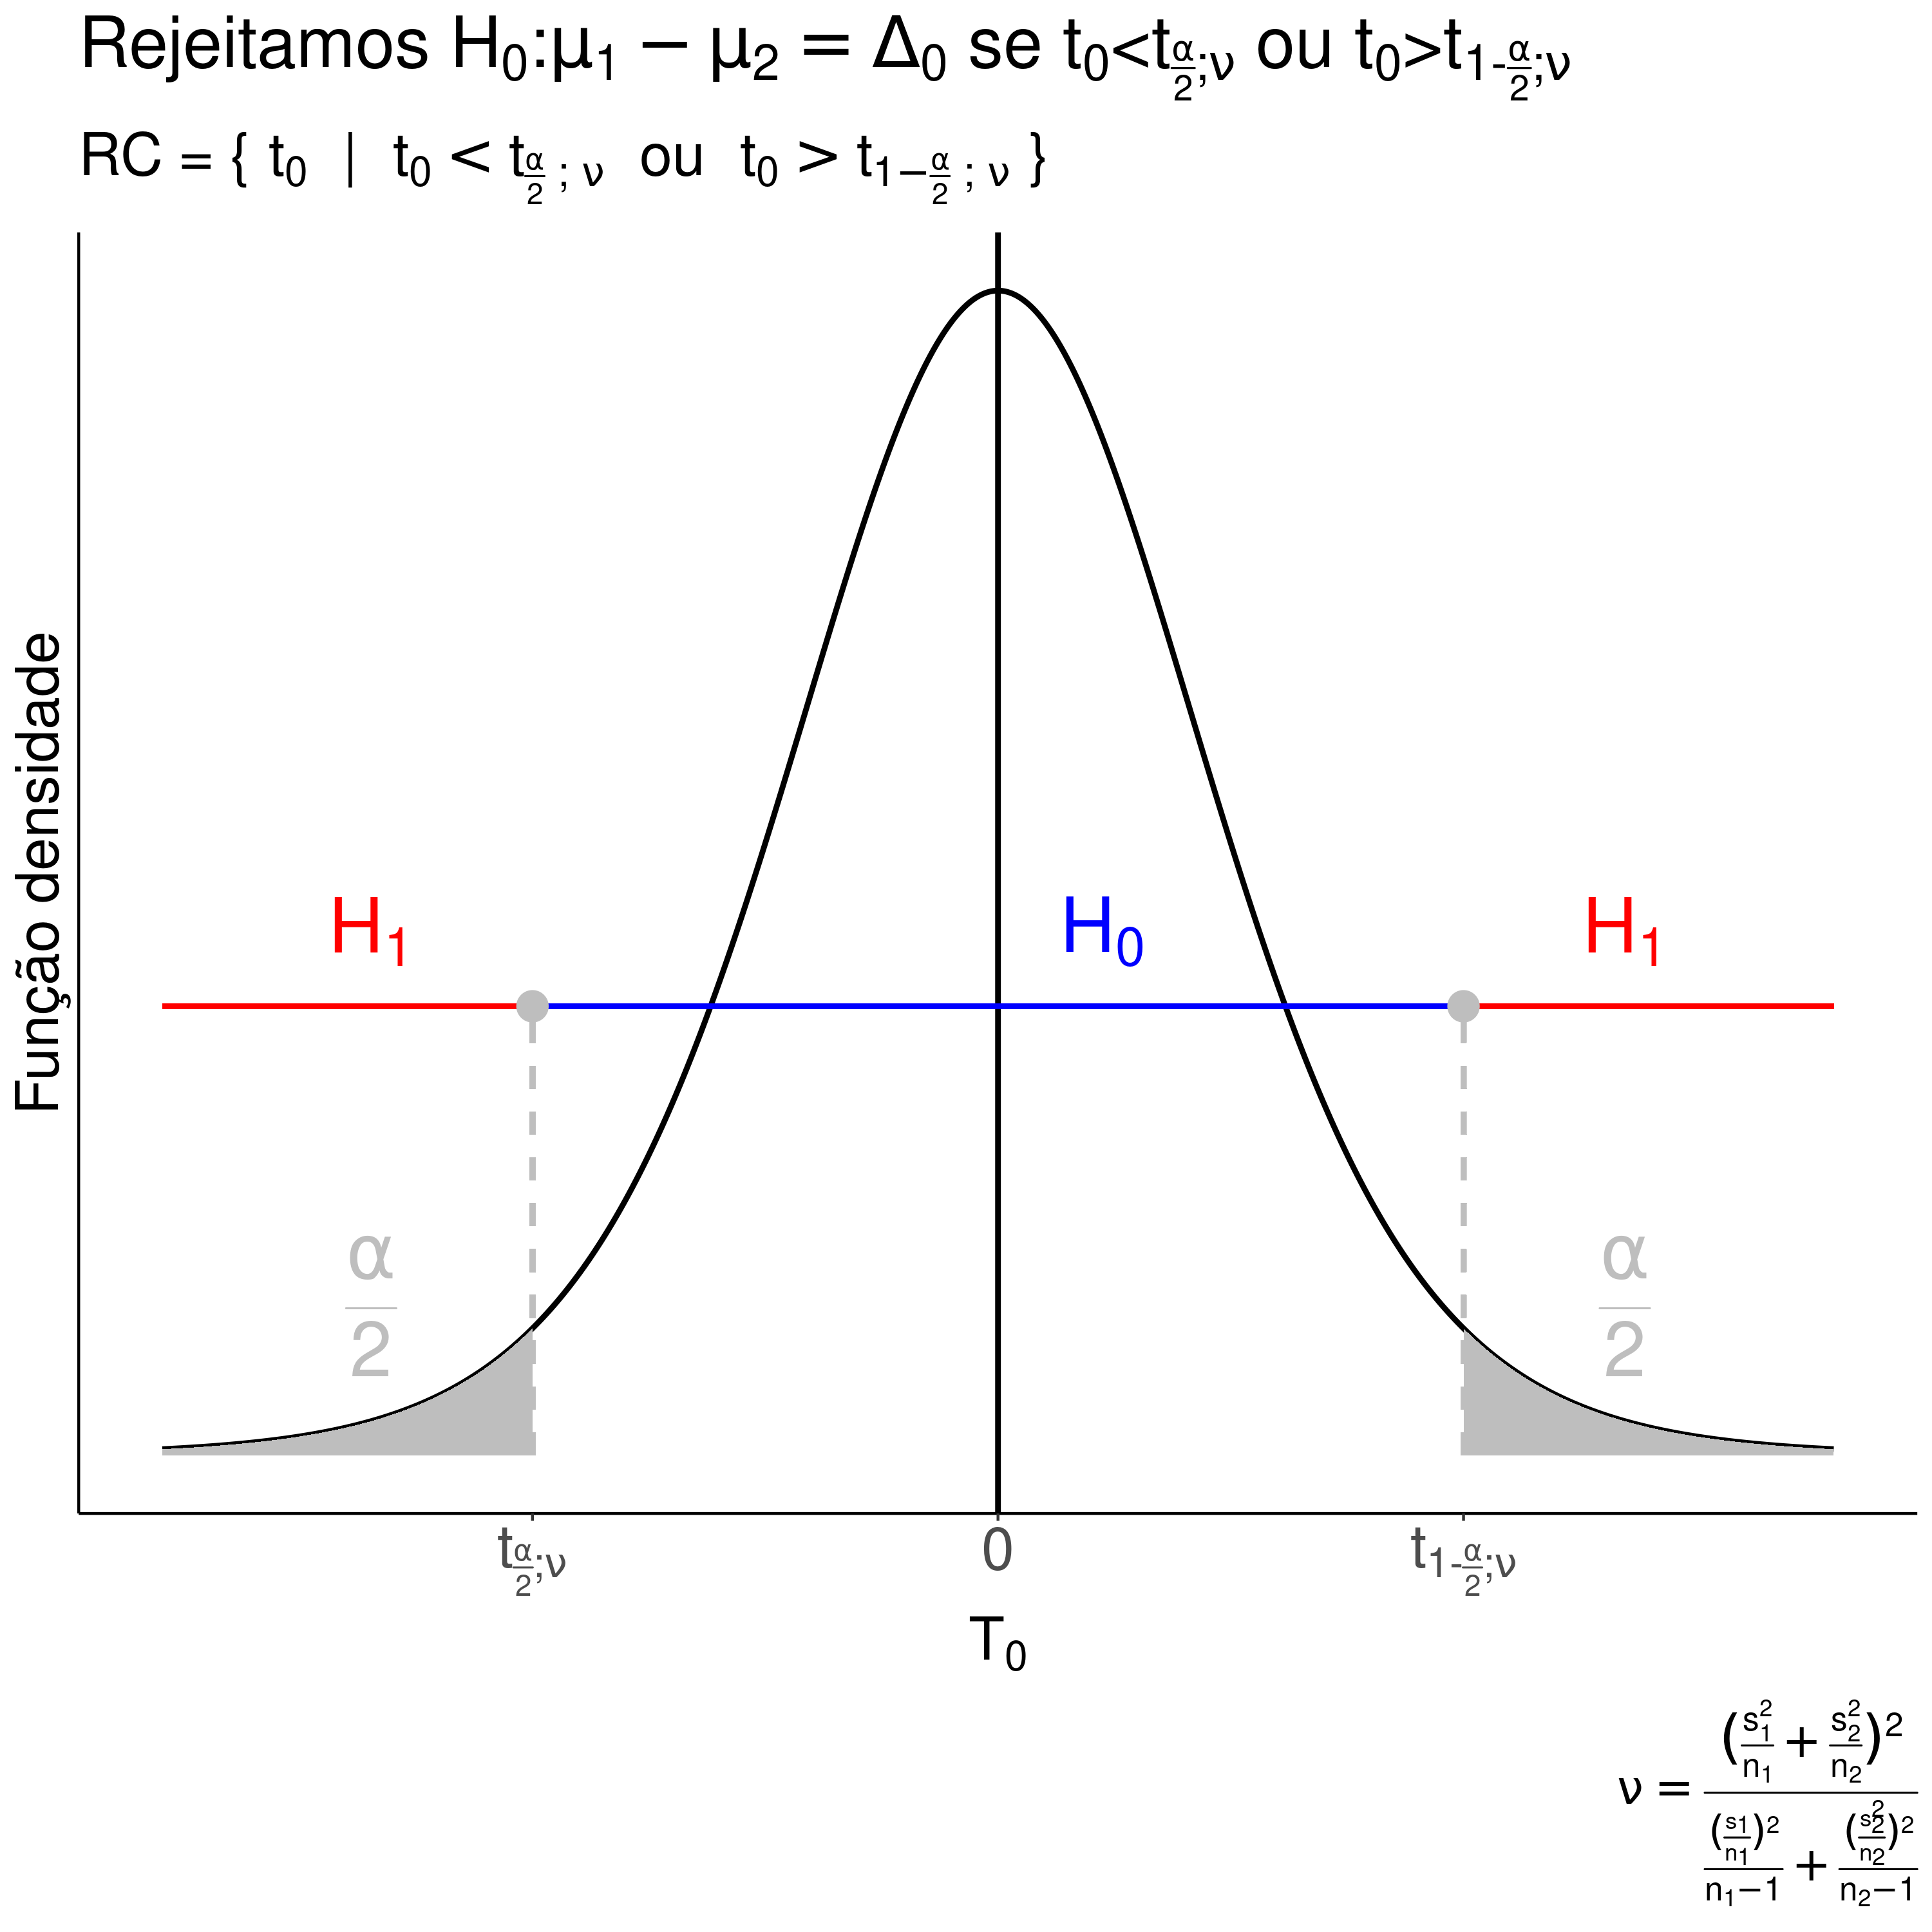
\includegraphics[width=0.32\linewidth]{figures/2-pop-normal-s2-unknown-different-bilateral.png} \label{fig:2-pop-normal-s2-unknown-different-bilateral}} \hfill
	\subfloat[][Teste bilateral.]{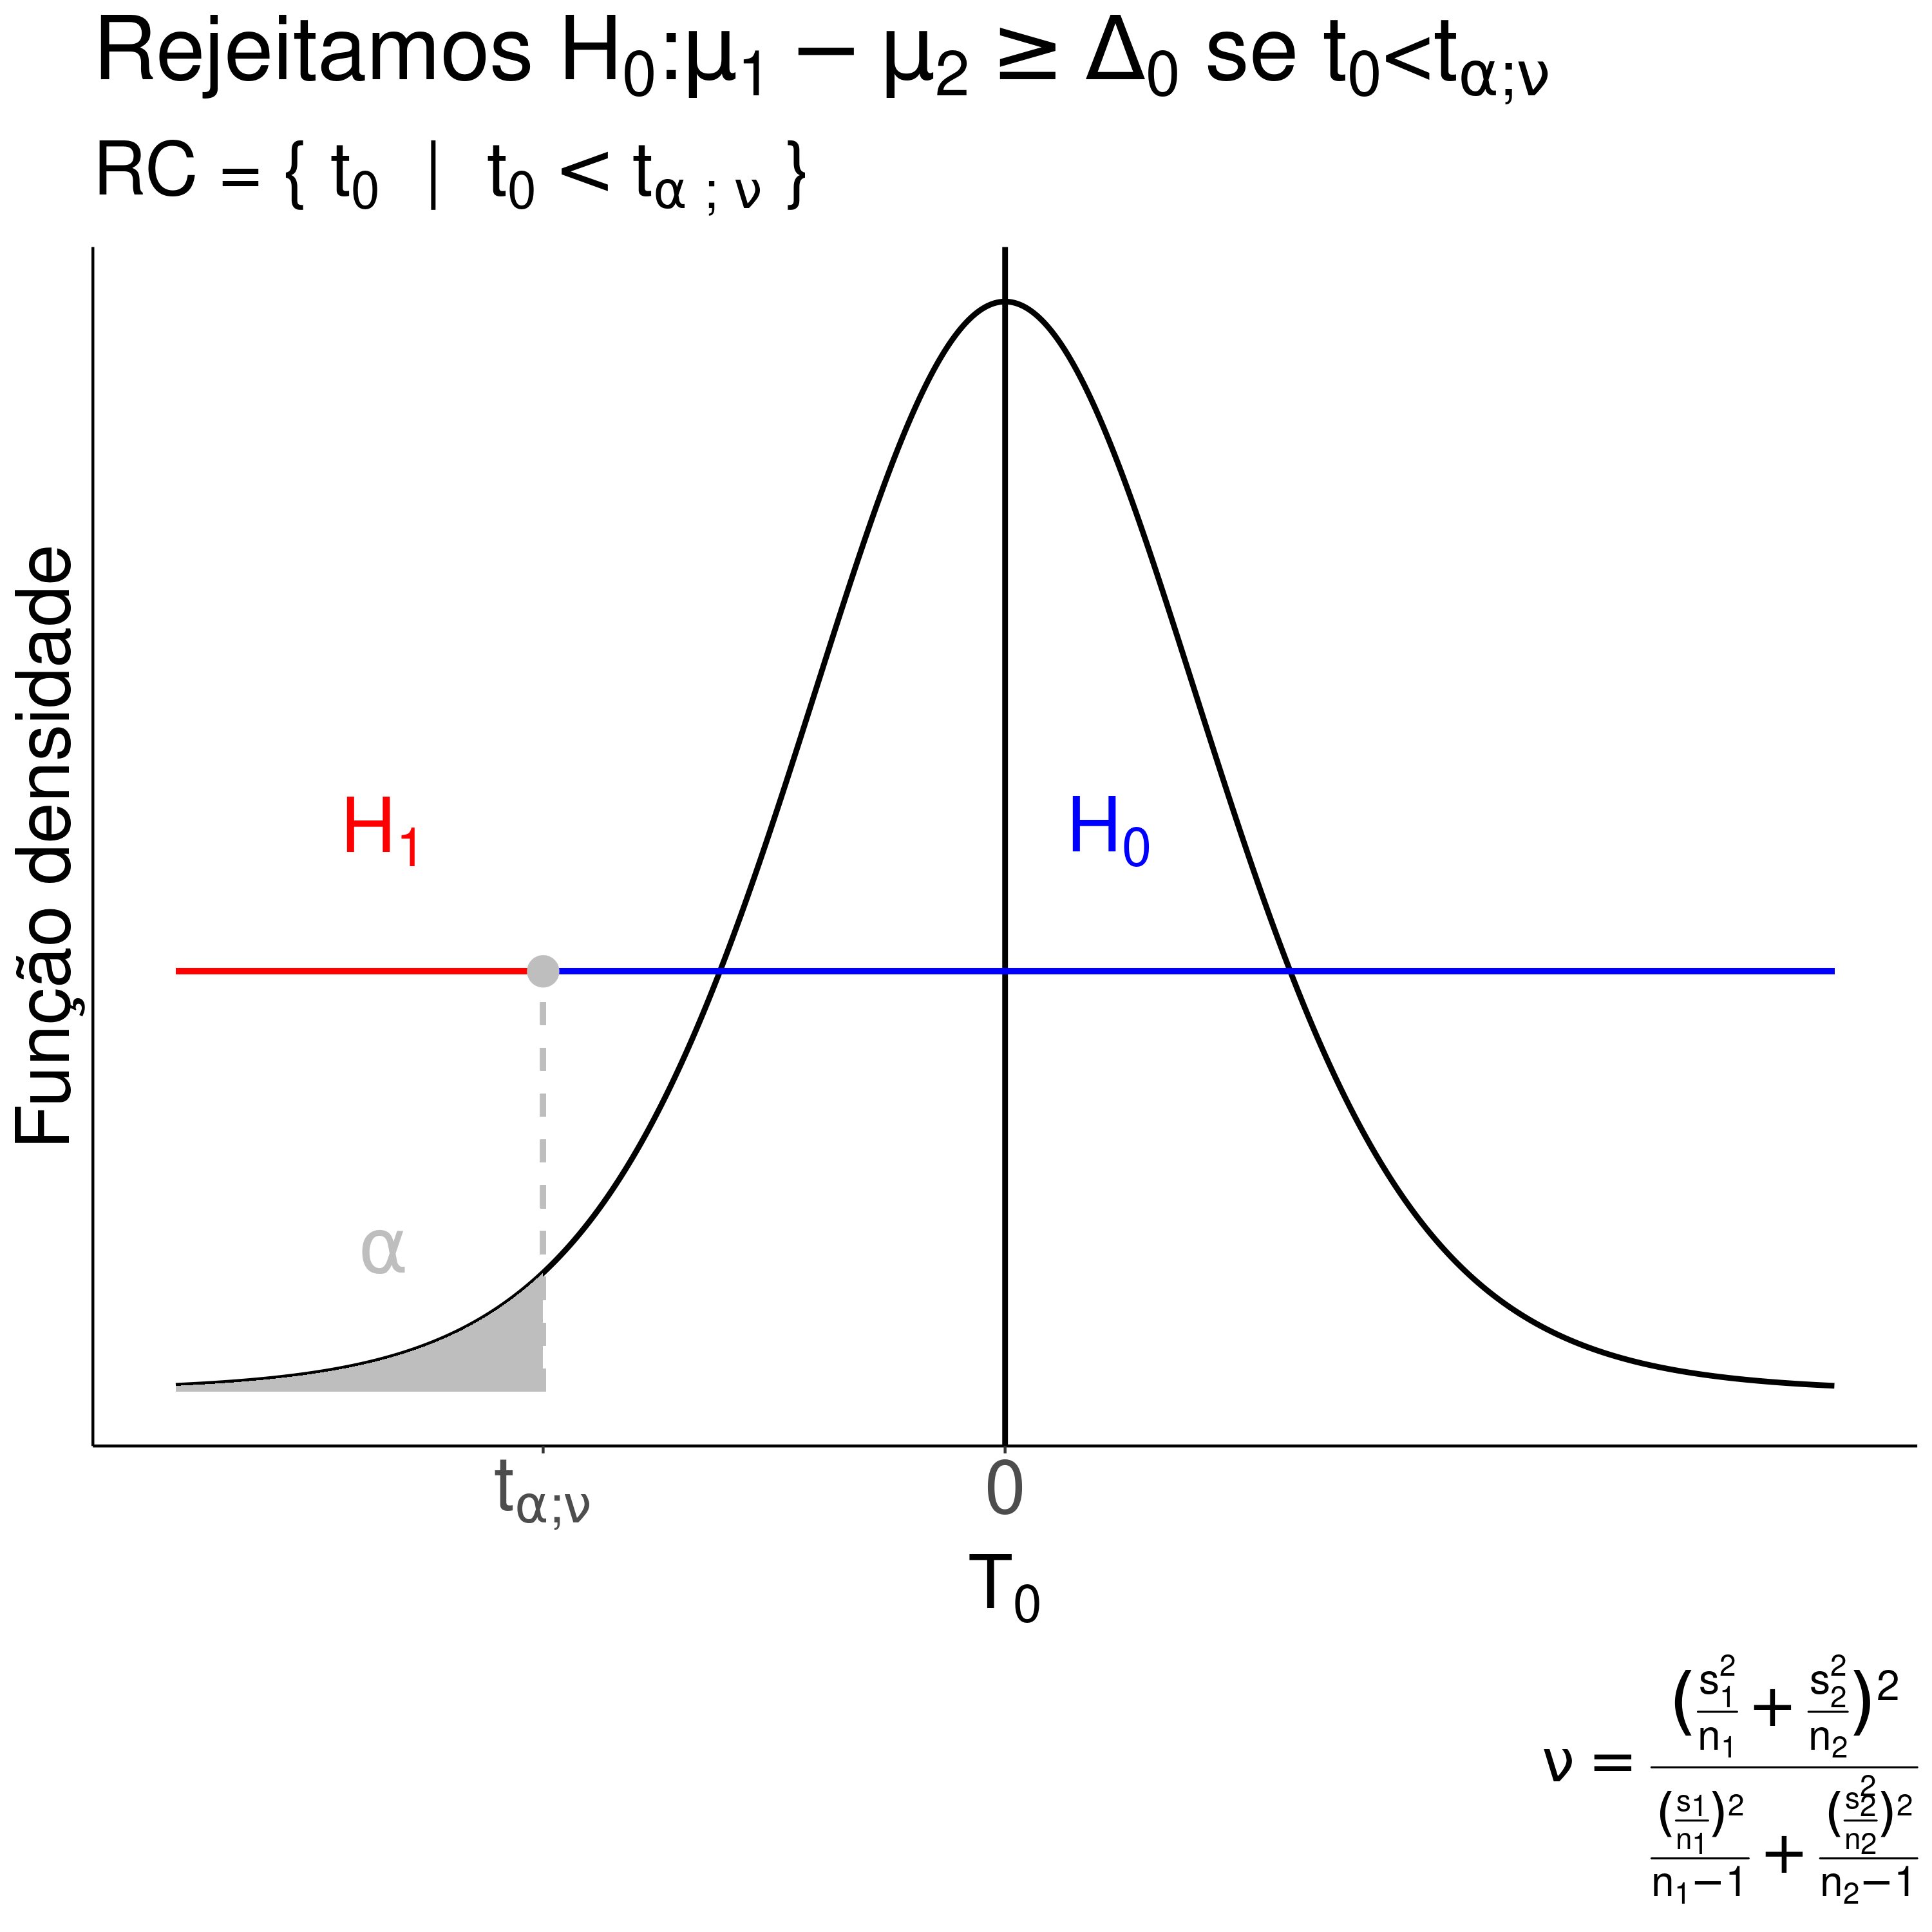
\includegraphics[width=0.32\linewidth]{figures/2-pop-normal-s2-unknown-different-h1-lower.png} \label{fig:2-pop-normal-s2-unknown-different-h1-lower}} \hfill
	\subfloat[][Teste bilateral.]{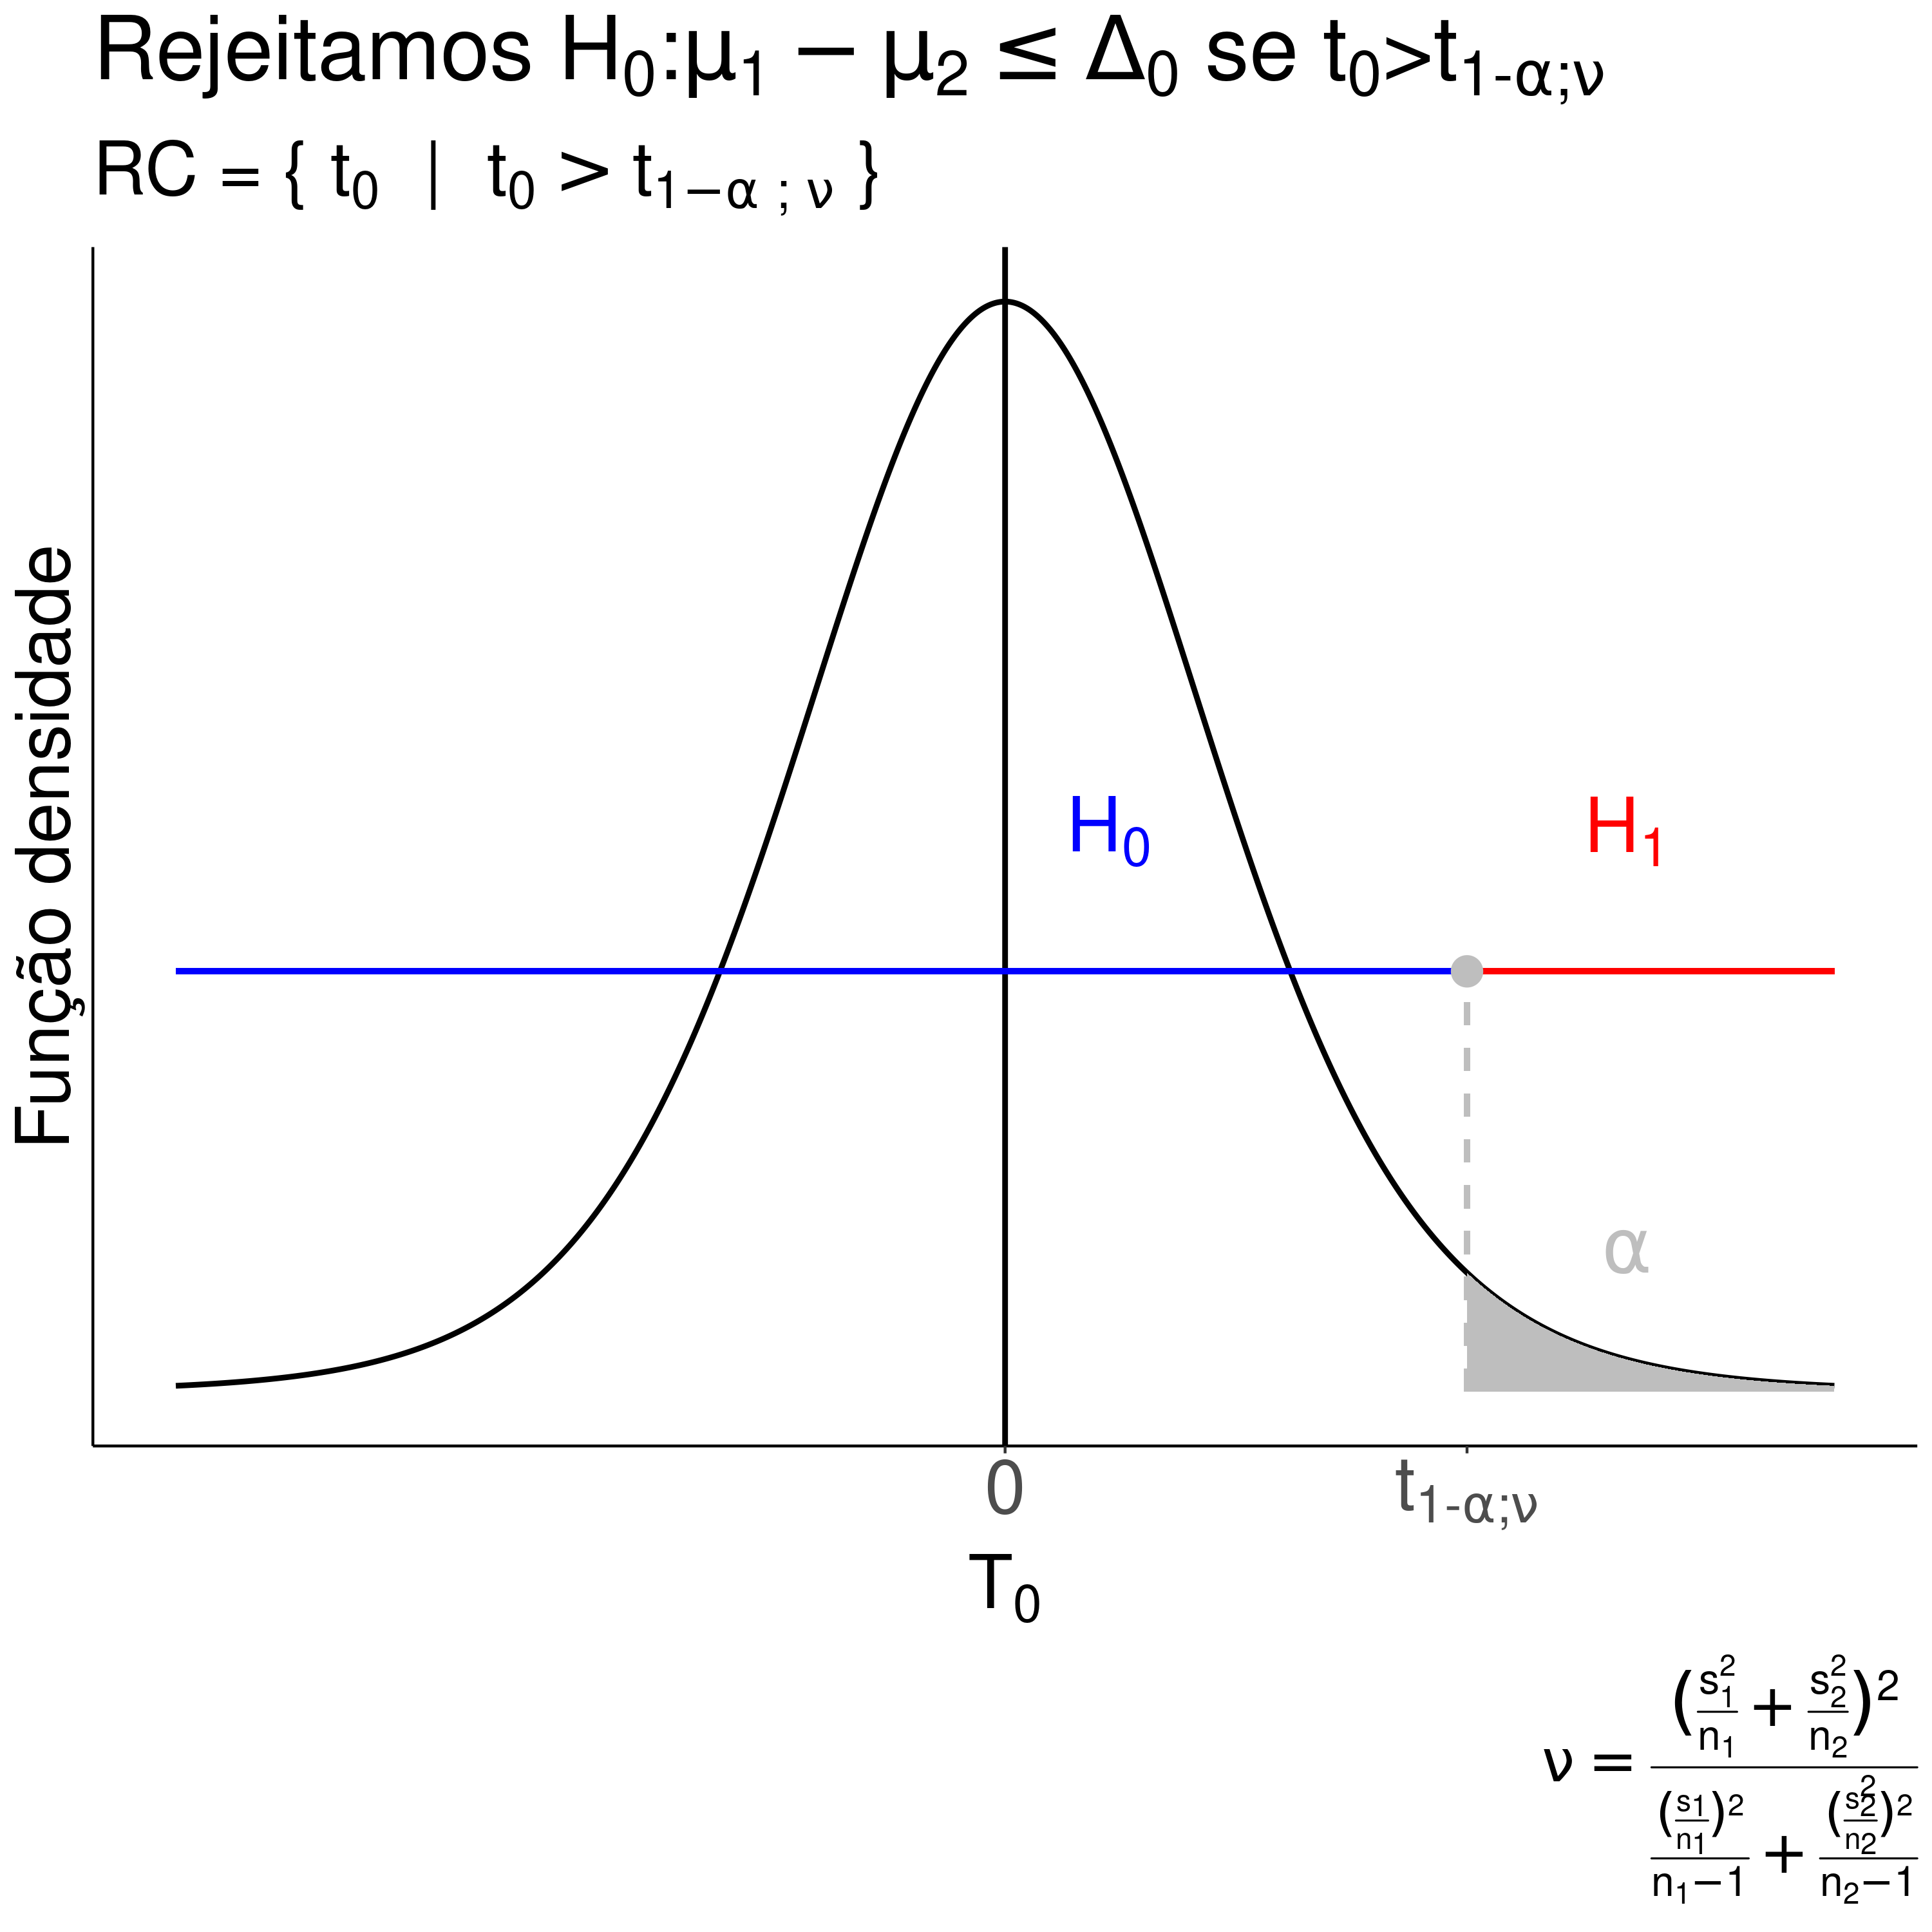
\includegraphics[width=0.32\linewidth]{figures/2-pop-normal-s2-unknown-different-h1-upper.png} \label{fig:2-pop-normal-s2-unknown-different-h1-upper}} 
	\caption{Região crítica para comparar médias de populações normais com variâncias desconhecidas e diferentes.}
\end{figure}

$\nu = \frac{\left( \frac{s_1^2}{n_1} + \frac{s_2^2}{n_2} \right)^2}{ \frac{\left( \nicefrac{s_1^2}{n_1} \right)^2}{n_1-1} + \frac{\left( \nicefrac{s_2^2}{n_2} \right)^2}{n_2-1} }$ é chamada de equação de Welch–Satterthwaite.


\textcolor{important}{Se você não sabe se as variâncias das populações são iguais, aconselha-se assumir que as variâncias são diferentes.}
\end{frame}

\begin{frame}{Comparação de médias $\mu_1$ e $\mu_2$ de duas populações.}

\footnotesize

\begin{itemize}
	\item Na Figura~\ref{fig:2-pop-normal-s2-unknown-different-bilateral}, testamos $H_0: \mu_1 - \mu_2 = \Delta_0$ versus $H_1: \mu_1 - \mu_2 \neq \Delta_0$. Rejeitamos $H_0$ se $t_0 = \frac{\bar{x}_1 - \bar{x}_1 - \Delta_0}{ \sqrt{ \frac{s_1^2}{n_1} + \frac{s_2^2}{n_2} } } \in  RC=\{t_0 \mid t_0 < t_{\frac{\alpha}{2};\nu} \allowbreak \mbox{ ou } t_0 > t_{1-\frac{\alpha}{2};\nu} \}$, em que $P\left(t_{\nu} \leq t_{\frac{\alpha}{2}; \nu} \right) = \frac{\alpha}{2}$ e $P\left(t_{\nu} \leq t_{1-\frac{\alpha}{2}; \nu} \right) = 1 - \frac{\alpha}{2}$;
	\vfill
	
	\item Na Figura~\ref{fig:2-pop-normal-s2-unknown-different-h1-lower}, testamos $H_0: \mu_1 - \mu_2 \leq \Delta_0 $ versus $H_1: \mu_1 - \mu_2 > 0$. Rejeitamos $H_0$ se $t_0 = \frac{\bar{x}_1 - \bar{x}_1 - \Delta_0}{ \sqrt{ \frac{s_1^2}{n_1} + \frac{s_2^2}{n_2} } } \in \allowbreak RC=\{t_0 \mid t_0 > t_{1-\alpha; \nu}  \}$, em que $P\left(t_{\nu} \leq  t_{1-\alpha;\nu} \right) =1- \alpha$;
	\vfill
	
	\item Na Figura~\ref{fig:2-pop-normal-s2-unknown-different-h1-upper}, testamos $H_0: \mu_1 - \mu_2 \geq \Delta_0$ versus $H_1: \mu_1 - \mu_2  < 0$. Rejeitamos $H_0$ se $t_0 = \frac{\bar{x}_1 - \bar{x}_1 - \Delta_0}{ \sqrt{ \frac{s_1^2}{n_1} + \frac{s_2^2}{n_2} } } \in \allowbreak RC=\{t_0 \mid t_0 < t_{\alpha;\nu}  \}$, em que $P\left(t_{\nu} \leq t_{\alpha;\nu} \right) = \alpha$.
\end{itemize}
Note que $\nu = \frac{\left( \frac{s_1^2}{n_1} + \frac{s_2^2}{n_2} \right)^2}{ \frac{\left( \frac{s_1^2}{n_1} \right)^2}{n_1-1} + \frac{\left( \frac{s_2^2}{n_2} \right)^2}{n_2-1} }$ (equação de Welch–Satterthwaite) e $t_{\alpha;\nu}$, $t_{1-\alpha;\nu}$, $t_{\frac{\alpha}{2};\nu}$ e $t_{1-\frac{\alpha}{2};\nu}$ são chamados de valores críticos. Se $\nu$ não é um número inteiro, arrendonde $\nu$ para o número inteiro mais próximo.

Alguns livros, chamam essa comparação de médias quando as variâncias populacionais distintas de teste de Welch.

\normalsize

\end{frame}

\begin{frame}{Comparação de médias $\mu_1$ e $\mu_2$ de duas populações.}

\begin{block}{Exemplo}
	A concentração de arsênico no sistema de abastecimento de água é um sério risco para a saúde público. Um estudo em 2001 	mediu concentrações de arsênico em partes por bilhão ($ppb$) na região metropolitana de Phoenix nos Estados Unido da América em 10 comunidades urbanas e em 10 comunidades rurais e os dados estão na Tabela~\ref{tab:arsenico}. Assuma que a concentração de arsênico tem distribuição normal. Existe diferença entre o campo e a cidade nas concentrações de arsênico? Use $\alpha=5\%$ e calcule o valor-p.
\end{block}

\begin{table}[htbp]
	\centering
	\scalebox{0.55}{
	\begin{tabular}{l|l}
		\toprule[0.05cm]
		Região urbana & Região rural \\ 
		$\bar{x}_1=12,5; s_1 = 7,63$ & $\bar{x}_2=27,5, s_2=15,3$\\ \midrule[0,025cm]
		Phoenix, 3 & Rimrock, 48 \\ 
		Chandler, 7 & Goodyear, 44 \\ 
		Gilbert, 25 & New River, 40 \\ 
		Glendale, 10 & Apache Junction, 38 \\ 
		Mesa, 15 & Buckeye, 33 \\ 
		Paradise Valley, 6 & Nogales, 21 \\ 
		Peoria, 12 & Black Canyon City, 20 \\ 
		Scottsdale, 25 & Sedona, 12 \\ 
		Tempe, 15 & Payson, 1 \\ 
		Sun City, 7 & Casa Grande, 18 \\ \bottomrule[0.05cm]
	\end{tabular}
	}
	\caption{Concentração de arsênico para 20 comunidades na região metropolitana de Phoenix.}
	\label{tab:arsenico}
\end{table}
\end{frame}

\begin{frame}{Comparação de médias $\mu_1$ e $\mu_2$ de duas populações.}
\small
\begin{block}{Solução}
	Primeiro, precisamos checar se as variâncias são iguais. 
	
	\textbf{Passo 1)} Queremos decidir entre duas hipóteses: $H_0: \frac{\sigma_1^2}{\sigma_2^2} = 1$ e $H_1: \frac{\sigma_1^2}{\sigma_2^2} \neq 1$;
	
	\textbf{Passo 2)} Vamos usar $\alpha=5\%$;
	
	\textbf{Passo 3)} Rejeitamos $H_0$ se $F_0 = \frac{s_1^2}{s_2^2}$ for pequeno ou grande. Ou seja, $RC = \left\{ f_0 \mid f_0 < f_{\frac{\alpha}{2}; n_1-1, n_2-1} \mbox{ ou } f_0 < f_{1-\frac{\alpha}{2}, n_1-1, n_2-1} \right\}$;
	
	\textbf{Passo 4)} Vamos encontrar os valores críticos:
	\begin{itemize}
		\item $P(F_{n_1-1, n_2-1} \leq f_{1-\frac{\alpha}{2}; n_1-1, n_2-1}) = P(F_{9, 9} \leq f_{0,975; 9, 9}) = 1-\frac{\alpha}{2} = 0,975$, então $f_{0,975; 9, 9}=4,026$;
		\item $P(F_{n_2-1, n_1-1} \leq f_{1-\frac{\alpha}{2}; n_2-1, n_1-1}) = P(F_{9, 9} \leq f_{0,975; 9, 9}) = 1-\frac{\alpha}{2} = 0,975$, então $f_{0,975; 9, 9}=4,026$;
		\item $f_{\frac{\alpha}{2}; n_1-1, n_2-1} = \frac{1}{f_{1-\frac{\alpha}{2}; n_2-1, n_1-1}}=\frac{1}{4,026}=0,2483$.
	\end{itemize}

	\textbf{Passo 5)} Note que $s_1 = 7,63$, $s_2=15,3$ e $f_0= \frac{s_1^2}{s_2^2} = 0,2487$, então $f_0 \not\in RC$ e não rejeitamos $H_0$. Ou seja, ao nível de significância de $\alpha=5\%$, as variâncias da concentração de arsênico nas regiões urbana e rual são iguais.
	
\end{block}
\normalsize
\end{frame}

\begin{frame}{Comparação de médias $\mu_1$ e $\mu_2$ de duas populações.}

\scriptsize
\begin{block}{Solução}
	\textbf{Passo 1)} Queremos decidir entre as hipóteses: $H_0: \mu_1 - \mu_2 = \Delta_0=0$ e $H_1: \mu_1 - \mu_2 \neq \Delta_0=0$;
	
	\textbf{Passo 2)} Nível de significância $\alpha=5\%$;
	
	\textbf{Passo 3)} Rejeitamos $H_0$ se $\lvert T_0 \rvert = \left\lvert \frac{\bar{X}_1 - \bar{X}_2 - \Delta_0}{\sqrt{\frac{s_1^2}{n_1} + \frac{s_2^2}{n_2}}} \right\rvert$ for grande. Ou seja, $RC = \left\{ t_0 \mid t_0 < t_{\frac{\alpha}{2}; \nu} \mbox{ ou } t_0 < t_{1-\frac{\alpha}{2};\nu} \right\}$, em que $\nu = \frac{\left(\frac{s_1^2}{n_1} + \frac{s_2^2}{n_2} \right)^2}{\frac{\left(\nicefrac{s_1^2}{n_1}\right)^2}{n_1-1} + \frac{\left(\nicefrac{s_2^2}{n_2}\right)^2}{n_2-1}}$;
	
	\textbf{Passo 4)} Vamos encontrar os valores críticos:
	\begin{itemize}
		\item $\nu = \frac{\left(\frac{s_1^2}{n_1} + \frac{s_2^2}{n_2} \right)^2}{\frac{\left(\nicefrac{s_1^2}{n_1}\right)^2}{n_1-1} + \frac{\left(\nicefrac{s_2^2}{n_2}\right)^2}{n_2-1}} = 13,22$, usamos $\nu=13$;
		\item $P(t_{\nu} \leq t_{\frac{\alpha}{2}; \nu}) = P(t_{13} \leq t_{0,025; 13}) = \frac{\alpha}{2} = 0,025$, então $t_{0,025; 13} = -2,160$;
		\item $P(t_{\nu} \leq t_{\frac{\alpha}{2}; \nu}) = P(t_{13} \leq t_{0,975; 13}) =1- \frac{\alpha}{2} = 0,975$, então $t_{0,975; 13} = 2,160$;
	\end{itemize}

	\textbf{Passo 5)} Note que $x_1=12,5$, $x_2=27,5$, $s_1=7,63$, $s_2=15,3$, $\Delta_0=0$, $t_0 = \frac{\bar{x}_1 - \bar{x}_2 - \Delta_0}{\sqrt{\frac{s_1^2}{n_1} + \frac{s_2^2}{n_2}}} = \frac{7,63 - 15,3}{\sqrt{\frac{7,63^2}{10} + \frac{15,3^2}{10}}}=-2,77 \in RC$, então Rejeitamos $H_0$ ao nível de significância $\alpha=5\%$. Ou seja, a concentração de arsênico presente no serviço de fornecimento de água é diferente nas regiões urbanas e rurais.
\end{block}
\normalsize

\end{frame}

\begin{frame}{Comparação de médias $\mu_1$ e $\mu_2$ de duas populações.}

\begin{block}{Solução (valor-p)}
	O valor-p é dado por
	$$p = P(\lvert T_0 \rvert > \lvert t_0 \rvert  \mid H_0) = 2 \cdot \left[1 - P(T_\nu \leq \lvert t_0 \rvert)\right].$$
	
	Note que $x_1=12,5$, $x_2=27,5$, $s_1=7,63$, $s_2=15,3$, $\Delta_0=0$, $t_0 = \frac{\bar{x}_1 - \bar{x}_2 - \Delta_0}{\sqrt{\frac{s_1^2}{n_1} + \frac{s_2^2}{n_2}}} = \frac{7,63 - 15,3}{\sqrt{\frac{7,63^2}{10} + \frac{15,3^2}{10}}}=-2,77$ e $\nu = \frac{\left(\frac{s_1^2}{n_1} + \frac{s_2^2}{n_2} \right)^2}{\frac{\left(\nicefrac{s_1^2}{n_1}\right)^2}{n_1-1} + \frac{\left(\nicefrac{s_2^2}{n_2}\right)^2}{n_2-1}} = 13,22$, então o valor é dado por
	\begin{align*}
	p &=2\cdot \left[1- P(t_\nu \leq \lvert  t_0\rvert)\right]\\
	&=2\cdot \left[ P(t_{13,22} \leq \lvert -2,77 \rvert)\right]\\
	&= 2 \cdot \left[ 1 - 0,9921 \right]\\
	&= 0,0158.
	\end{align*}
	
	Como $p = 0,0158 < \alpha=0,05$, rejeitamos $H_0$. Ou seja a concentração de arsênico presente no serviço de fornecimento de água é diferente nas comunidades urbanas e rurais.
\end{block}

\end{frame}

\begin{frame}{Comparação de médias $\mu_1$ e $\mu_2$ de duas populações.}

\begin{block}{Exemplo}
	Um pesquisador tem duas variáveis normais e independentes e ele deseja checar se as médias das duas variáveis normais são iguais. Algumas informações deste experimento estão na Tabela~\ref{tab:experimento-h1-upper}. Complete a Tabela~\ref{tab:experimento-h1-upper}. A média da população 2 é maior que a média da população 1? Use $\alpha=5\%$. Calcule o valor-p.
\end{block}

\begin{table}[htbp]
	\centering
	\begin{tabular}{c|c|c|c|c}
		\toprule[0.1cm]
		$n_1$ & $\bar{x}_1$ & $s_1$ & $n_2$ & $\bar{x}_2$\\ \midrule[0.025cm]
		$15$ & $30,5$ & $2,51$ & $25$ & $52,6$\\ \midrule[0.05cm]
		$s_2$ & $\sigma_1^2 = \sigma_2^2?$ & $\mu_2 - \mu_1 > 0?$ & $t_0$ & valor-p\\ \midrule[0.025cm]
		$13,3$ & & & & \\ \bottomrule[0.1cm]
	\end{tabular}
	\caption{Algumas informações do experimento.}
	\label{tab:experimento-h1-upper}
\end{table}

\end{frame}

\begin{frame}{Comparação de médias $\mu_1$ e $\mu_2$ de duas populações.}

\begin{block}{Solução}
	Primeiro vamos verificar se variâncias populacionais são iguais.
	
	\textbf{Passo 1)} Queremos testar as hipóteses: $H_0: \frac{\sigma_1^2}{\sigma_2^2} = 1$ e $H_1:\frac{\sigma_1^2}{\sigma_2^2} \neq 1$;
	
	\textbf{Passo 2)} Nível de significância $\alpha=5\%$;
	
	\textbf{Passo 3)} Rejeito $H_0$ se $F_0 = \frac{S_1^2}{S_2^2}$ for grande ou pequeno. Ou seja, $RC= \left\{ f_0 \mid f_0 < f_{\frac{\alpha}{2}; n_1-1, n_2-1} \mbox{ ou } f_0 < f_{1-\frac{\alpha}{2};n_1-1, n_2-1} \right\}$;
	
	\textbf{Passo 4)} Vamos encontrar os valores críticos:
	\begin{itemize}
		\item $P(F_{n_1-1, n_2-1} \leq f_{1-\frac{\alpha}{2}; n_1-1, n_2-1}) = P(F_{14, 24} \leq f_{0,975; 14, 24}) = 1-\frac{\alpha}{2} = 0,975$, então $f_{0,975; 14, 24} = 2,468$;
		\item $P(F_{n_2-1, n_1-1} \leq f_{1-\frac{\alpha}{2}; n_2-1, n_1-1}) = P(F_{24, 14} \leq f_{0,975; 24, 14}) = 1-\frac{\alpha}{2} = 0,975$, então $f_{0,975; 24, 14} = 2,789$;
		\item $f_{\frac{\alpha}{2};n_1-1, n_2-1} = f_{0,025; 14, 24} = \frac{1}{f_{1-\frac{\alpha}{2}; n_2-1, n_1-1}} = \frac{1}{f_{0,975; 14, 24}} = \frac{1}{2,789} =0,3586$.
	\end{itemize}

	\textbf{Passo 5)} Como $s_1=2,51$, $s_2 = 13,3$, $f_0 = \frac{s_1^2}{s_2^2} = 0,04 \in RC$, então rejeitamos $H_0$. Ou seja, ao nível de significância $\alpha=5\%$, as duas variâncias populacionais são distintas.
\end{block}
\end{frame}

\begin{frame}{Comparação de médias $\mu_1$ e $\mu_2$ de duas populações.}

\begin{block}{Solução}
	\textbf{Passo 1)} Pelo enunciado, queremos testar as hipóteses: $H_0: \mu_2 - \mu_1 \leq \Delta_0 = 0$ e $H_1: \mu_2 - \mu_1 > \Delta_0 = 0$;
	
	\textbf{Passo 2)} Nível de significância $\alpha=5\%$;
	
	\textbf{Passo 3)} Rejeito $H_0$ se $t_0 = \frac{\bar{X}_2 - \bar{X}_1 -\Delta_0}{\sqrt{\frac{s_1^2}{n_1} + \frac{s_2^2}{n_2}}}$ for grande. Ou esteja, $RC = \left\{ t_0 \mid t_0 > t_{1-\alpha, \nu} \right\}$;
	
	\textbf{Passo 4)} Vamos encontrar o valor crítico:
	\begin{itemize}
		\item $\nu = \frac{\left( \frac{s_1^2}{n_1} + \frac{s_2^2}{n_2} \right)^2}{\frac{\left(\nicefrac{s_1^2}{n_1}\right)^2}{n_1-1} + \frac{\left(\nicefrac{s_2^2}{n_2}\right)^2}{n_2-1}} = 26,77$, então usaremos $\nu=27$;
		\item $P(t_\nu \leq t_{1-\alpha;\nu}) = P(t_{27} \leq t_{0,95; 27})= 1-\alpha = 0,95$, então $t_{0,95; 27} = 1,703$.
	\end{itemize}

	\textbf{Passo 5)} Como $n_1=15$, $\bar{x}_1=30,5$, $s_1 = 2,51$, $n_2=25$, $\bar{x}_2 = 52,6$, $s_2 = 13,3$ e $\Delta_0=0$, então $t_0 = \frac{\bar{x}_2 - \bar{x}_1 - \Delta_0}{\sqrt{\frac{s_1^2}{n_1} + \frac{s_2^2}{n_2}}}= \frac{52,6 - 30,5}{\sqrt{\frac{2,51^2}{15} + \frac{13,3^2}{25}}} = 2,87 \in RC$, então rejeitamos $H_0$.
\end{block}
\end{frame}

\begin{frame}{Comparação de médias $\mu_1$ e $\mu_2$ de duas populações.}

\begin{block}{Solução (valor-p)}
	O valor-p é calculado através de
	$$p=P(T_0 > t_0 \mid H_0) = 1 - P(t_\nu \leq t_0),$$
	em que $\nu = \frac{\left( \frac{s_1^2}{n_1} + \frac{s_2^2}{n_2} \right)^2}{\frac{\left(\nicefrac{s_1^2}{n_1}\right)^2}{n_1-1} + \frac{\left(\nicefrac{s_2^2}{n_2}\right)^2}{n_2-1}}$.
	
	Como $n_1 = 15$, $\bar{x}_1 = 30,5$, $s_1=2,51$, $n_2 = 25$, $\bar{x}_2 = 52,6$, $s_2 = 13,3$, $t_0 = 2,87$, $\nu = 26,77$, então o valor-p é dado por
	\begin{align*}
		p &= 1 - P(t_\nu \leq t_0)\\
		&= 1 - P(t_{26,77} \leq 2,87)\\
		&= 0,004.
	\end{align*}
	
	Como $p=0,004 < 0,05 = \alpha$, rejeitamos $H_0$ ao nível de significância $\alpha=5\%$.
\end{block}
\end{frame}

\begin{frame}{Comparação de médias $\mu_1$ e $\mu_2$ de duas populações.}

\begin{block}{Exemplo}
	Dois fornecedores fabricam um material de borracha usados em aplicações automotivas. Esta parte de borracha sofrerá um desgaste abrasivo no uso, e o engenheiro decide comparar as partes. Vinte e cinco partes de cada fornecedor foram coletadas, e o desgaste foi medido depois de 1000 ciclos. Para a companhia 1 a média e o desvio padrão são $x_1 = 20$ e $s_1 = 2$ miligramas  por $1000$ ciclos , e para a companhia 2 a média e o desvio padrão são $\bar{x}_2=15$ e $s_2=8$ miligramas por $1000$ ciclos. Os dados suportam a hipótese do engenheiro que o desgaste da companhia 2 é menor? Use $\alpha=5\%$. Calcule o valor-p.
\end{block}
 
\end{frame}

\begin{frame}{Comparação de médias $\mu_1$ e $\mu_2$ de duas populações.}

\begin{block}{Solução}
	Primeiro vamos verificar se variâncias populacionais são iguais.
	
	\textbf{Passo 1)} Queremos testar as hipóteses: $H_0: \frac{\sigma_1^2}{\sigma_2^2} = 1$ e $H_1:\frac{\sigma_1^2}{\sigma_2^2} \neq 1$;
	
	\textbf{Passo 2)} Nível de significância $\alpha=5\%$;
	
	\textbf{Passo 3)} Rejeito $H_0$ se $F_0 = \frac{S_1^2}{S_2^2}$ for grande ou pequeno. Ou seja, $RC= \left\{ f_0 \mid f_0 < f_{\frac{\alpha}{2}; n_1-1, n_2-1} \mbox{ ou } f_0 < f_{1-\frac{\alpha}{2};n_1-1, n_2-1} \right\}$;
	
	\textbf{Passo 4)} Vamos encontrar os valores críticos:
	\begin{itemize}
		\item $P(F_{n_1-1, n_2-1} \leq f_{1-\frac{\alpha}{2}; n_1-1, n_2-1}) = P(F_{24, 24} \leq f_{0,975; 24, 24}) = 1-\frac{\alpha}{2} = 0,975$, então $f_{0,975; 24, 24} = 2,269$;
		\item $P(F_{n_2-1, n_1-1} \leq f_{1-\frac{\alpha}{2}; n_2-1, n_1-1}) = P(F_{24, 24} \leq f_{0,975; 24, 24}) = 1-\frac{\alpha}{2} = 0,975$, então $f_{0,975; 24, 24} = 2,269$;
		\item $f_{\frac{\alpha}{2};n_1-1, n_2-1} = f_{0,025; 24, 24} = \frac{1}{f_{1-\frac{\alpha}{2}; n_2-1, n_2-1}} = \frac{1}{f_{0,975; 24, 24}} = \frac{1}{2,269} =0,4407$.
	\end{itemize}
	
	\textbf{Passo 5)} Como $s_1=2,51$, $s_2 = 13,3$, $f_0 = \frac{s_1^2}{s_2^2} = 0,04 \in RC$, então rejeitamos $H_0$. Ou seja, ao nível de significância $\alpha=5\%$, as duas variâncias populacionais são distintas.
\end{block}
\end{frame}

\begin{frame}{Comparação de médias $\mu_1$ e $\mu_2$ de duas populações.}

\small
\begin{block}{Solução}
	\textbf{Passo 1)} Queremos testar as hipóteses: $H_0: \mu_2 - \mu_1 \geq \Delta_0=0$ e $H_1: \mu_2 - \mu_1 < \Delta_0=0$;
	
	\textbf{Passo 2)} Nível de significância $\alpha=5\%$;
	
	\textbf{Passo 3)} Rejeitamos $H_0$ se $t_0=\frac{\bar{X}_2 - \bar{X}_1 - \Delta_0}{\sqrt{\frac{s_1^2}{n_1} + \frac{s_2^2}{n_2}}} $ for pequeno. Ou seja, $RC = \left\{ t_0 \mid t_0 < t_{\alpha; \nu} \right\}$;
	
	\textbf{Passo 4)} Vamos encontrar o valor crítico:
	\begin{itemize}
		\item $\nu = \frac{\left( \frac{s_1^2}{n_1} + \frac{s_2^2}{n_2} \right)^2}{\frac{\left(\nicefrac{s_1^2}{n_1}\right)^2}{n_1-1} + \frac{\left(\nicefrac{s_2^2}{n_2}\right)^2}{n_2-1}} = \frac{\left( \frac{2^2}{25} + \frac{8^2}{25} \right)^2}{\frac{\left(\nicefrac{2^2}{25}\right)^2}{25-1} + \frac{\left(\nicefrac{8^2}{25}\right)^2}{25-1}} = 26,99$, então vamos usar $\nu = 27$;
		\item $P(t_\nu \leq t_{\alpha, \nu}) = P(t_{27} \leq t_{0,05; 27})$, então $t_{0,05; 27} = -1,703$.
	\end{itemize}

	\textbf{Passo 5)} Como $n_1=n_2=25$, $\bar{x}_1=20$, $\bar{x}_2=15$, $s_1=2$, $s_2=8$ e $t_0 = \frac{\bar{x}_2 - \bar{x}_1- \Delta_0}{\sqrt{\frac{s_1^2}{n_1} + \frac{s_2^2}{n_2}}} = \frac{15 - 20  - 0}{\sqrt{\frac{2^2}{25} + \frac{8^2}{25}}}=-2,38 \in RC$, e rejeitamos $H_0$. 
	
	Ou seja, ao nível de significância $\alpha=5\%$, o desgaste da parte de borracha fornecida pela companhia 2 é menor.
\end{block}
\normalsize

\end{frame}

\begin{frame}{Comparação de médias $\mu_1$ e $\mu_2$ de duas populações.}

\begin{block}{Solução (valor-p)}
	O valor-p é dado por
	$$p = P (T_0 < t_0 \mid H_0) = P(t_\nu < t_0).$$
	
	Note que $n_1=n_2=25$, $\bar{x}_1=20$, $\bar{x}_2=15$, $s_1=2$, $s_2=8$ e $t_0 = \frac{\bar{x}_2 - \bar{x}_1- \Delta_0}{\sqrt{\frac{s_1^2}{n_1} + \frac{s_2^2}{n_2}}} = \frac{15 - 20  - 0}{\sqrt{\frac{2^2}{25} + \frac{8^2}{25}}}=-2,38$ e $\nu = \frac{\left( \frac{s_1^2}{n_1} + \frac{s_2^2}{n_2} \right)^2}{\frac{\left(\nicefrac{s_1^2}{n_1}\right)^2}{n_1-1} + \frac{\left(\nicefrac{s_2^2}{n_2}\right)^2}{n_2-1}} = \frac{\left( \frac{2^2}{25} + \frac{8^2}{25} \right)^2}{\frac{\left(\nicefrac{2^2}{25}\right)^2}{25-1} + \frac{\left(\nicefrac{8^2}{25}\right)^2}{25-1}} = 26,99$, então o valor-p é dado por
	\begin{align*}
		p &= P(t_\nu \leq t_0)\\
		&= (P_{22,99} \leq -2,38)\\
		&= 0,013.
	\end{align*}
	
	Como $p=0,013 < \alpha=0,05$, rejeitamos $H_0$, ou seja, o desgaste da parte de borracha pela companhia 2 é menor.
\end{block}

\end{frame}


\subsection{Poder e tamanho da amostra.}

\begin{frame}{Poder do teste: $H_0:\mu_1 - \mu_2 = \Delta_0$ e $H_1: \mu_1 - \mu_2 \neq \Delta_0$.}

\tiny

Imagine que
\begin{itemize}
	\item Hipóteses: $H_0: \mu_1 - \mu_2 = \Delta_0$ e $H_1: \mu_1 -  \mu_2 \neq \Delta_0$;
	\item $H_1$ é verdade, então $\Delta = \mu_1-\mu_2 \neq \Delta_0$;
	\item As variâncias $\sigma_1^2$  e $\sigma_2^2$ das duas populações são diferentes e desconhecidas;
	\item $T_0 = \frac{\bar{X}_1 - \bar{X}_2 - \Delta_0}{ \sqrt{ \frac{s_1^2}{n_1} + \frac{s_2^2}{n_2} } } \sim t_{n_1+n_2-2}\left( \frac{\mu_1 - \mu_2 - \Delta_0}{\sqrt{\frac{\sigma_1^2 + \sigma_1^2}{2}} \sqrt{\frac{1}{n_1} + \frac{1}{n_2}}} \right)$. Chamamos $d = \frac{\mu_1 - \mu_2 - \Delta_0}{\sqrt{\frac{\sigma_1^2 + \sigma_1^2}{2}}}$ de tamanho do efeito;
	\item Ao nível de significância $\alpha$, temos $RC = \{ t_0 \mid t_0 < t_{\frac{\alpha}{2};\nu} \mbox{ ou } t_{1-\frac{\alpha}{2};\nu} < t_0  \}$.
\end{itemize}
\vfill	

Poder do teste é dado
\begin{align*}
\textcolor{important}{1-\beta} &=1 - \left[P\left( t_{\frac{\alpha}{2};\nu} \leq T_0 \leq t_{1-\frac{\alpha}{2};\nu} \mid H_1 \right)\right] = 1 - \left[P\left( t_{\frac{\alpha}{2};\nu} \leq T_0 \leq t_{1-\frac{\alpha}{2};\nu} \mid \Delta \neq \Delta_0 \right)\right]\\
&\approx \textcolor{important}{1 - P\left( t_{n}\left( \frac{\lvert \mu_1 - \mu_2 - \Delta_0 \rvert}{\sqrt{\frac{\sigma_1^2 + \sigma_1^2}{2}} \sqrt{\frac{1}{n_1} + \frac{1}{n_2}}} \right) \leq t_{1-\frac{\alpha}{2};n} \right)+P\left( t_{n}\left( \frac{\lvert \mu_1 - \mu_2 - \Delta_0 \rvert}{\sqrt{\frac{\sigma_1^2 + \sigma_1^2}{2}} \sqrt{\frac{1}{n_1} + \frac{1}{n_2}}} \right) \leq t_{\frac{\alpha}{2};n} \right).}
\end{align*}
em que $n = n_1 + n_2 - 2$. A \textcolor{important}{Função Poder}, dado o tamanho da amostra $n$, é uma função das médias populacionais na hipótese alternativa  $\pi: \mathbb{R} - \{\Delta_0\} \longrightarrow [0,1]$ dada por
\begin{align*}
\pi(\delta) = 1 - P\left( t_{n}\left( \frac{\lvert \mu_1 - \mu_2 - \Delta_0 \rvert}{\sqrt{\frac{\sigma_1^2 + \sigma_1^2}{2}} \sqrt{\frac{1}{n_1} + \frac{1}{n_2}}} \right) \leq t_{1-\frac{\alpha}{2};n} \right)+P\left( t_{n}\left( \frac{\lvert \mu_1 - \mu_2 - \Delta_0 \rvert}{\sqrt{\frac{\sigma_1^2 + \sigma_1^2}{2}} \sqrt{\frac{1}{n_1} + \frac{1}{n_2}}} \right) \leq t_{\frac{\alpha}{2};n} \right),
\end{align*}
em que $n=n_1+n_2-2$ e $\Delta = \mu_1 - \mu_2, \Delta \in \mathbb{R} - \{\Delta_0 \}$. Alguns livros chamam a Função Poder de \textcolor{important}{Curva de Característica Operacional.}

\normalsize

\end{frame}


\begin{frame}[fragile]{Tamanho da amostra: $H_0:\mu_1 - \mu_2 = \Delta_0$ e $H_1: \mu_1 - \mu_2 \neq \Delta_0$.}

\footnotesize

Imagine que
\begin{itemize}
\item Hipóteses: $H_0: \mu_1 - \mu_2 = \Delta_0$ e $H_1: \mu_1 -  \mu_2 \neq \Delta_0$;
\item $H_1$ é verdade, então $\Delta = \mu_1-\mu_2 \neq \Delta_0$;
\item As variâncias $\sigma_1^2$  e $\sigma_2^2$ das duas populações são iguais e desconhecidas. Usamos $S_d^2 = \frac{(n_1-1)s_1^2 + (n_2-1)s_2^2}{n_1+n_2-2}$;
\item $T_0 = \frac{\bar{X}_1 - \bar{X}_2 - \Delta_0}{ S_d \sqrt{ \frac{1}{n_1} + \frac{1}{n_2} } } \sim t_{n_1+n_2-2}\left( \frac{\mu_1 - \mu_2 - \Delta_0}{\frac{\sigma_1^2 + \sigma_1^2}{2} \sqrt{\frac{1}{n_1} + \frac{1}{n_2}}} \right)$, em que $\frac{\mu_1 - \mu_2 - \Delta_0}{\frac{\sigma_1^2 + \sigma_1^2}{2} \sqrt{\frac{1}{n_1} + \frac{1}{n_2}}}$ é o parâmetro de não-centralidade da distribuição t-Student;
\item Ao nível de significância $\alpha$, temos $RC = \{ t_0 \mid t_0 < t_{\frac{\alpha}{2};\nu} \mbox{ ou } t_{1-\frac{\alpha}{2};\nu} < t_0  \}$.
\end{itemize}
\vfill

Considere $1-\beta$, $\alpha$, $n_1=n_2=n$, então o tamanho \sout{mínimo} da amostra é solução da seguinte equação
\scriptsize
\begin{align}\label{eq:pwr-t-test-hetero-bilateral}
1-\beta = 1 - P\left( t_{2n-2}\left( \frac{\lvert \mu_1 - \mu_2 - \Delta_0 \rvert}{\sqrt{\frac{\sigma_1^2 + \sigma_1^2}{2}} \sqrt{\frac{2}{n}}} \right) \leq t_{1-\frac{\alpha}{2};2n-2} \right)+P\left( t_{2n-2}\left( \frac{\lvert \mu_1 - \mu_2 - \Delta_0\rvert}{\sqrt{\frac{\sigma_1^2 + \sigma_1^2}{2}} \sqrt{\frac{2}{n}}} \right) \leq t_{\frac{\alpha}{2};2n-2} \right).
\end{align}

A equação~\eqref{eq:pwr-t-test-hetero-bilateral} é resolvida usando métodos numéricos que estão implementados em diversos \textit{softwares}.
\begin{description}
	\item[No R] \lstinline|pwr_sigma_2pop|
\end{description}
Esta função está no pacote \lstinline|power|, que pode ser instalado usando o pacote \lstinline|devtools|: \lstinline|devtools::install_github("gilberto-sassi/power")|.

\normalsize
\end{frame}

\begin{frame}{Poder do teste: $H_0:\mu_1 - \mu_2 = \Delta_0$ e $H_1: \mu_1 - \mu_2 \neq \Delta_0$.}

\begin{block}{Exemplo}
	A concentração de arsênico no sistema de abastecimento de água é um sério risco para a saúde público. Um estudo em 2001 	mediu concentrações de arsênico em partes por bilhão ($ppb$) na região metropolitana de Phoenix nos Estados Unido da América em 10 comunidades urbanas e em 10 comunidades rurais. Assuma que a concentração de arsênico tem distribuição normal. Além disso, considere que a média e o desvio padrão da concentração de arsênico na região urbana são $\mu_1 = 13 ppb$ e $\sigma_1=8 ppb$ e a média e o desvio padrão da concentração de arsênico na região rural são $\mu_2=28 ppb$ e $\sigma_2=16 ppb$. Calcule o poder do teste. Use $\alpha=5\%$.	
\end{block}

\end{frame}

\begin{frame}[fragile]{Poder do teste: $H_0:\mu_1 - \mu_2 = \Delta_0$ e $H_1: \mu_1 - \mu_2 \neq \Delta_0$.}

\scriptsize
\begin{block}{Solução}
	\textbf{Passo 1)} Queremos testar as hipóteses: $H_0: \mu_1 - \mu_2 = \Delta_0 = 0$ e $H_0: \mu_1 - \mu_2 \neq \Delta_0 = 0$;
	
	\textbf{Passo 2)} Nível de significância $\alpha=5\%$;
	
	Vamos encontrar os quantis da distribuição t-Student:
	\begin{itemize}
		\item $P(t_{n_1+n_2-2} \leq t_{\frac{\alpha}{2}; n_1+n_2-2}) = P(t_{18} \leq t_{0,025; 18})=\frac{\alpha}{2} = 0,025$, então $t_{0,025; 18} = -2,101$;
		\item $P(t_{n_1+n_2-2} \leq t_{\frac{\alpha}{2}; n_1+n_2-2}) = P(t_{18} \leq t_{0,975; 18})=1-\frac{\alpha}{2} = 0,975$, então $t_{0,975; 18} = 2,101$.
	\end{itemize}

	Como $n_1=n_2=10$, $\mu_1=13$, $\sigma_1=8$, $\mu_2=28$, $\sigma_2=16$, $\Delta_0 = 0$, então o parâmetro de não-centralidade é $\mu = \frac{\lvert\mu_1 - \mu_2 - \Delta_0\rvert}{\sqrt{\frac{\sigma_1^2 + \sigma_1^2}{2}} \sqrt{\frac{1}{n_1} + \frac{1}{n_2}}} = 2,65$. Então, o poder do teste é dado por
	\begin{align*}
	1-\beta &= 1 - P\left( t_{n_1+n_2-2}\left(\mu \right) \leq t_{1-\frac{\alpha}{2};n_1+n_2-2} \right)+P\left( t_{n_1+n_2-2}\left( \mu \right) \leq t_{\frac{\alpha}{2};n_1+n_2-2} \right)\\
	&= 1 - P (t_{18}(2,65) \leq 2,101) + P (t_{18}(2,65) \leq -2,101) = 0,7082.
	\end{align*}
\end{block}

\begin{lstlisting}[language = C, caption = Código no R.]
pwr_t_test_2pop_hetero(sigma1 = 8, sigma2 = 16, delta = 13 - 28,
		delta0 = 0, n1 = 10, n2 = 10, pwr = NULL, alternative = "two.sided",
		sig_level = 0.05)
\end{lstlisting}

\end{frame}

\begin{frame}{Tamanho da amostra: $H_0:\mu_1 - \mu_2 = \Delta_0$ e $H_1: \mu_1 - \mu_2 \neq \Delta_0$.}

\begin{block}{Exemplo}
	A concentração de arsênico no sistema de abastecimento de água é um sério risco para a saúde público. Um estudo em deseja medir concentrações de arsênico em partes por bilhão ($ppb$) na região metropolitana de Phoenix nos Estados Unido da América em comunidades urbanas e em comunidades rurais. Assuma que a concentração de arsênico tem distribuição normal. Além disso, considere que a média e o desvio padrão da concentração de arsênico na região urbana são $\mu_1 = 13 ppb$ e $\sigma_1=8 ppb$ e a média e o desvio padrão da concentração de arsênico na região rural são $\mu_2=28 ppb$ e $\sigma_2=16 ppb$. Quantas amostras de água das comunidades urbanas e rurais da região metropolitana de Phoenix precisamos coletar para termos $1-\beta=99\%$. Use $\alpha=5\%$.	
\end{block}
\end{frame}

\begin{frame}[fragile]{Tamanho da amostra: $H_0:\mu_1 - \mu_2 = \Delta_0$ e $H_1: \mu_1 - \mu_2 \neq \Delta_0$.}

\begin{block}{Solução}
	\textbf{Passo 1)} Queremos testar as hipóteses: $H_0: \mu_1 - \mu_2 = \Delta_0$ e $H_1: \mu_1 - \mu_2 \neq \Delta_0$;
	
	\textbf{Passo 2)} Nível de significância $\alpha=5\%$;
	
	Como $1-\beta=0,99$, $\alpha=0,05$, $\mu_1=13$, $\sigma=8$, $\mu_2=28$, $\sigma_2=16$, então o tamanho \sout{mínimo} da amostra é solução da seguinte equação
	\tiny
	\begin{align*}
		1-\beta &=  1 - P\left( t_{2n-2}\left( \frac{\lvert \mu_1 - \mu_2 - \Delta_0 \rvert}{\sqrt{\frac{\sigma_1^2 + \sigma_1^2}{2}} \sqrt{\frac{2}{n}}} \right) \leq t_{1-\frac{\alpha}{2};2n-2} \right)+P\left( t_{2n-2}\left( \frac{\lvert \mu_1 - \mu_2 - \Delta_0\rvert}{\sqrt{\frac{\sigma_1^2 + \sigma_1^2}{2}} \sqrt{\frac{2}{n}}} \right) \leq t_{\frac{\alpha}{2};2n-2} \right)\\
		&=  1 - P\left( t_{2n-2}\left( \frac{\lvert 13 - 28 - 0 \rvert}{\sqrt{\frac{8^2 + 16^2}{2}} \sqrt{\frac{2}{n}}} \right) \leq t_{0,975;2n-2} \right)+P\left( t_{2n-2}\left( \frac{\lvert 13 - 28 - 0\rvert}{\sqrt{\frac{8^2 + 16^2}{2}} \sqrt{\frac{2}{n}}} \right) \leq t_{0,025;2n-2} \right).
	\end{align*}
	\normalsize
	
	Então, precisamos coletar 28 amostras das comunidades urbanas e 28 amostras das comunidades rurais.
\end{block}

\begin{lstlisting}[language = C, caption = Código no R.]
pwr_t_test_2pop_hetero(sigma1 = 8, sigma2 = 16, delta = 13 - 28,
		delta0 = 0, n1 = NULL, n2 = NULL, pwr = 0.99,
		alternative = "two.sided", sig_level = 0.05)
\end{lstlisting}

\end{frame}

\begin{frame}{Poder do teste: $H_0:\mu_1 - \mu_2 \leq \Delta_0$ e $H_1: \mu_1 - \mu_2 > \Delta_0$.}

\tiny

Imagine que
\begin{itemize}
	\item Hipóteses: $H_0: \mu_1 - \mu_2 \leq \Delta_0$ e $H_1: \mu_1 -  \mu_2 > \Delta_0$;
	\item $H_1$ é verdade, então $\Delta = \mu_1-\mu_2 \neq \Delta_0$;
	\item As variâncias $\sigma_1^2$  e $\sigma_2^2$ das duas populações são diferentes e desconhecidas;
	\item $T_0 = \frac{\bar{X}_1 - \bar{X}_2 - \Delta_0}{ \sqrt{ \frac{s_1^2}{n_1} + \frac{s_2^2}{n_2} } } \sim t_{n_1+n_2-2}\left( \frac{\mu_1 - \mu_2 - \Delta_0}{\sqrt{\frac{\sigma_1^2 + \sigma_1^2}{2}} \sqrt{\frac{1}{n_1} + \frac{1}{n_2}}} \right)$. Chamamos $d = \frac{\mu_1 - \mu_2 - \Delta_0}{\sqrt{\frac{\sigma_1^2 + \sigma_1^2}{2}}}$ de tamanho do efeito;
	\item Ao nível de significância $\alpha$, temos $RC = \{ t_0 \mid t_0 > t_{1-\alpha;\nu} \}$.
\end{itemize}
\vfill	

Poder do teste é dado
\begin{align*}
\textcolor{important}{1-\beta} &=1 - \left[P\left( T_0 \leq t_{1-\alpha;\nu} \mid H_1 \right)\right] = 1 - \left[P\left( T_0 \leq t_{1-\alpha;\nu} \mid \Delta \neq \Delta_0 \right)\right]\\ 
&\approx \textcolor{important}{1 - P\left( t_{n}\left( \frac{ \mu_1 - \mu_2 - \Delta_0 }{\sqrt{\frac{\sigma_1^2 + \sigma_1^2}{2}} \sqrt{\frac{1}{n_1} + \frac{1}{n_2}}} \right) \leq t_{1-\frac{\alpha}{2};n} \right).}
\end{align*}
em que $n = n_1 + n_2 - 1$. A \textcolor{important}{Função Poder}, dado o tamanho da amostra $n$, é uma função das médias populacionais na hipótese alternativa  $\pi: (\Delta_0, \infty) \longrightarrow [0,1]$ dada por
\begin{align*}
\pi(\delta) = 1 - P\left( t_{n}\left( \frac{ \mu_1 - \mu_2 - \Delta_0 }{\sqrt{\frac{\sigma_1^2 + \sigma_1^2}{2}} \sqrt{\frac{1}{n_1} + \frac{1}{n_2}}} \right) \leq t_{1-\frac{\alpha}{2};n} \right),
\end{align*}
em que $n=n_1+n_2-2$ e $\Delta = \mu_1 - \mu_2, \Delta \in (\Delta_0, \infty)$. Alguns livros chamam a Função Poder de \textcolor{important}{Curva de Característica Operacional.}

\normalsize

\end{frame}


\begin{frame}[fragile]{Tamanho da amostra: $H_0:\mu_1 - \mu_2 \leq \Delta_0$ e $H_1: \mu_1 - \mu_2 > \Delta_0$.}

\footnotesize

Imagine que
\begin{itemize}
	\item Hipóteses: $H_0: \mu_1 - \mu_2 \leq \Delta_0$ e $H_1: \mu_1 -  \mu_2 > \Delta_0$;
	\item $H_1$ é verdade, então $\Delta = \mu_1-\mu_2 \neq \Delta_0$;
	\item As variâncias $\sigma_1^2$  e $\sigma_2^2$ das duas populações são diferentes e desconhecidas;
	\item $T_0 = \frac{\bar{X}_1 - \bar{X}_2 - \Delta_0}{ \sqrt{ \frac{s_1^2}{n_1} + \frac{s_2^2}{n_2} } } \sim t_{n_1+n_2-2}\left( \frac{\mu_1 - \mu_2 - \Delta_0}{\sqrt{\frac{\sigma_1^2 + \sigma_1^2}{2}} \sqrt{\frac{1}{n_1} + \frac{1}{n_2}}} \right)$. Chamamos $d = \frac{\mu_1 - \mu_2 - \Delta_0}{\sqrt{\frac{\sigma_1^2 + \sigma_1^2}{2}}}$ de tamanho do efeito;
	\item Ao nível de significância $\alpha$, temos $RC = \{ t_0 \mid t_0 > t_{1-\alpha;\nu} \}$.
\end{itemize}
\vfill

Considere $1-\beta$, $\alpha$, $n_1=n_2=n$, então o tamanho \sout{mínimo} da amostra é solução da seguinte equação
\scriptsize
\begin{align}\label{eq:pwr-t-test-hetero-greater}
1-\beta = 1 - P\left( t_{2n-2}\left( \frac{ \mu_1 - \mu_2 - \Delta_0 }{\sqrt{\frac{\sigma_1^2 + \sigma_1^2}{2}} \sqrt{\frac{2}{n}}} \right) \leq t_{1-\frac{\alpha}{2};2n-2} \right).
\end{align}

A equação~\eqref{eq:pwr-t-test-hetero-bilateral} é resolvida usando métodos numéricos que estão implementados em diversos \textit{softwares}.
\begin{description}
	\item[No R] \lstinline|pwr_sigma_2pop|
\end{description}
Esta função está no pacote \lstinline|power|, que pode ser instalado usando o pacote \lstinline|devtools|: \lstinline|devtools::install_github("gilberto-sassi/power")|.

\normalsize
\end{frame}

\begin{frame}{Poder do teste: $H_0: \mu_2 - \mu_1 \leq \Delta_0$ e $H_1: \mu_2 - \mu_1 > \Delta_0.$}

\begin{block}{Exemplo}
	Um pesquisador tem duas variáveis normais e independentes e ele deseja checar se as médias das duas variáveis normais são iguais. Algumas informações deste experimento estão na Tabela~\ref{tab:experimento-h1-upper-power}. Complete a Tabela~\ref{tab:experimento-h1-upper-power}. A média da população 2 é maior que a média da população 1? Use $\alpha=5\%$. Calcule o valor-p.
\end{block}

\begin{table}[htbp]
	\centering
	\begin{tabular}{c|c|c|c|c|c|c|c}
		\toprule[0.05cm]
		$n_1$ & $n_2$ & $\mu_1$ & $\mu_2$ & $\sigma_1$ & $\sigma_2$ & $1-\beta$ & $\alpha$ \\ \midrule[0.025cm]
		 10 & 15 & 30 & 40 & 5  & 10 & & $5\%$ \\
		 \bottomrule[0.05cm]
	\end{tabular}
	\caption{Algumas informações do experimento.}
	\label{tab:experimento-h1-upper-power}
\end{table}
\end{frame}

\begin{frame}[fragile]{Poder do teste: $H_0: \mu_2 - \mu_1 \leq \Delta_0$ e $H_1: \mu_2 - \mu_1 > \Delta_0.$}

\scriptsize
\begin{block}{Solução}
	\textbf{Passo 1)} Queremos testar as seguintes: $H_0: \mu_2 - \mu_1 \leq \Delta_0$ e $H_1: \mu_1 - \mu_2 > \Delta_0$;
	
	\textbf{Passo 2)} Nível de significância $\alpha=5\%$;
	
	Note que $n_1=10$, $n_2=15$, $\mu_1=30$, $\mu_2=40$, $\sigma_1=5$, $\sigma_2=10$, $\alpha = 0,05$. Primeiro calculamos o quantil
	\begin{itemize}
		\item $P(t_{n_1+n_2-2} \leq t_{1-\frac{\alpha}{2}; n_1+n_2-2}) = P(t_{23} \leq t_{0,975; 23}) = 1- \frac{\alpha}{2} = 0,975$, então $t_{0,975; 23} = 2,069$.
	\end{itemize}

	Então, o poder do teste é dado por
	\begin{align*}
		1- \beta &= 1 - P\left( t_{n_1 + n_2 -2}\left( \frac{ \mu_2 - \mu_1 - \Delta_0 }{\sqrt{\frac{\sigma_1^2 + \sigma_1^2}{2}} \sqrt{\frac{1}{n_1} + \frac{1}{n_2}}} \right) \leq t_{1-\frac{\alpha}{2};n_1 + n_2 -2} \right)\\
		&= 1 - P\left( t_{23}\left( \frac{ 40 - 30 - 0 }{\sqrt{\frac{5^2 + 10^2}{2}} \sqrt{\frac{1}{10} + \frac{1}{15}}} \right) \leq 2,069 \right)= 0,9132.
	\end{align*}
\end{block}

\begin{lstlisting}[language = C, caption = Código no R.]
pwr_t_test_2pop_hetero(sigma1 = 5, sigma2 = 10, delta = 40 - 30,
		delta0 = 0, n1 = 10, n2 = 15, pwr = NULL,
		alternative = "greater", sig_level = 0.05)
\end{lstlisting}

\normalsize
\end{frame}

\begin{frame}{Tamanho da amostra: $H_0: \mu_2 - \mu_1 \leq \Delta_0$ e $H_1: \mu_2 - \mu_1 > \Delta_0.$}

\begin{block}{Exemplo}
	Um pesquisador planeja estudar duas variáveis normais e independentes e ele deseja checar se as médias das duas variáveis normais são iguais. Algumas informações deste experimento estão na Tabela~\ref{tab:experimento-h1-upper-sample-size}. Complete a Tabela~\ref{tab:experimento-h1-upper-sample-size}. Imagine que pesquisador deseja verificar se a média da população 2 é maior que a média da população 1, qual o poder do teste? Use $\alpha=5\%$. Calcule o valor-p.
\end{block}

\begin{table}[htbp]
	\centering
	\begin{tabular}{c|c|c|c|c|c|c}
		\toprule[0.05cm]
		$n_1=n_2=n$ & $\mu_1$ & $\mu_2$ & $\sigma_1$ & $\sigma_2$ & $1-\beta$ & $\alpha$ \\ \midrule[0.025cm]
		 & 30 & 40 & 5 & 10 & $99\%$ & $5\%$ \\
		\bottomrule[0.05cm]
	\end{tabular}
	\caption{Algumas informações do experimento.}
	\label{tab:experimento-h1-upper-sample-size}
\end{table}
\end{frame}

\begin{frame}[fragile]{Tamanho do teste: $H_0: \mu_2 - \mu_1 \leq \Delta_0$ e $H_1: \mu_2 - \mu_1 > \Delta_0.$}

\small
\begin{block}{Solução}
	\textbf{Passo 1)} Queremos testar as seguintes: $H_0: \mu_2 - \mu_1 \leq \Delta_0$ e $H_1: \mu_1 - \mu_2 > \Delta_0$;

	\textbf{Passo 1)} Nível de significância $\alpha=5\%$;
	
	Note que $n_1=n_2=n$, $\mu_1=30$, $\mu_2=40$, $\sigma_1=5$, $\sigma_2=10$, $1-\beta = 0,99$.	Então, o tamanho \sout{mínimo} de amostra é dado por
	\begin{align*}
		1- \beta &= 0,99 = 1 - P\left( t_{2n -2}\left( \frac{ \mu_2 - \mu_1 - \Delta_0 }{\sqrt{\frac{\sigma_1^2 + \sigma_1^2}{2}} \sqrt{\frac{2}{n}}} \right) \leq t_{1-\alpha;2n -2} \right)\\
		&= 1 - P\left( t_{2n -2}\left( \frac{ -30 + 40 - 0 }{\sqrt{\frac{5^2 + 10^2}{2}} \sqrt{\frac{2}{n}}} \right) \leq t_{0,95;2n -2} \right)
	\end{align*}	
	
	Então, precisamos coletar 21 observações da primeira variável e coletar 21 observações da segunda variável.
\end{block}

\begin{lstlisting}[language = C, caption = Código no R.]
pwr_t_test_2pop_hetero(sigma1 = 5, sigma2 = 10, delta = 40 - 30,
		delta0 = 0, n1 = NULL, n2 = NULL, pwr = 0.99,
		alternative = "greater", sig_level = 0.05)
\end{lstlisting}

\normalsize
\end{frame}



\subsection{Intervalo de confiança para diferenças de médias: $\mu_1 - \mu_2$. (Variâncias diferentes e desconhecidas.)}

\begin{frame}{Intervalo de confiança para $\mu_1 - \mu_2$.}

\normalsize

Sejam
\begin{itemize}
	\item $x_{1,1}, \dots, x_{1,n_1}$ valores amostrados da população 1 $N(\mu_1, \sigma_1^2)$;
	\item $x_{2,1}, \dots, x_{2,n_2}$ valores amostrados da população 2 $N(\mu_1, \sigma_1^2)$;
	\item as duas populações são independentes;
	\item As variâncias $\sigma_1^2$ e $\sigma_2^2$ são diferentes e desconhecidas; 
	\item $\gamma=1-\alpha$ é o coeficiente de confiança. (Geralmente, $\gamma=95\%$).
\end{itemize}

Note que $T = \frac{\bar{X}_1  - \bar{X}_2 -(\mu_1 - \mu_2) }{\sqrt{\frac{s_1^2}{n_1} + \frac{s_2^2}{n_2}}} \sim t_\nu$, em que $\nu = \frac{\left( \frac{s_1^2}{n_1} + \frac{s_2^2}{n_2} \right)^2}{\frac{\left(\nicefrac{s_1^2}{n_1}\right)^2}{n_1-1} + \frac{\left(\nicefrac{s_2^2}{n_2}\right)^2}{n_2-1}}$, e 
$$P\left( t_{\frac{\alpha}{2}; \nu} \leq \frac{\bar{X}_1  - \bar{X}_2 -(\mu_1 - \mu_2) }{\sqrt{\frac{s_1^2}{n_1} + \frac{s_2^2}{n_2}}} \leq t_{1-\frac{\alpha}{2}; \nu} \right) = 1 - \alpha,$$
Então o intervalo de confiança para $\Delta$ com coeficiente de confiança $\gamma=1-\alpha$ é dado por
{\scriptsize
	$$IC\left(\mu_1 - \mu_2; \gamma\right) = \left( t_{\frac{\alpha}{2}; \nu} \sqrt{\frac{s_1^2}{n_1} + \frac{s_2^2}{n_2}} + \bar{X}_1 - \bar{X}_2; t_{1-\frac{\alpha}{2}; \nu} \sqrt{\frac{s_1^2}{n_1} + \frac{s_2^2}{n_2}} + \bar{X}_1 - \bar{X}_2 \right).$$
}

\normalsize
\end{frame}

\begin{frame}{Comparação de médias $\mu_1$ e $\mu_2$ de duas populações.}

\begin{block}{Exemplo}
A concentração de arsênico no sistema de abastecimento de água é um sério risco para a saúde público. Um estudo realizado em 2001 	mediu concentrações de arsênico em partes por bilhão ($ppb$) na região metropolitana de Phoenix nos Estados Unido da América em 10 comunidades urbanas e em 10 comunidades rurais e os dados estão na Tabela~\ref{tab:arsenico_ic}. Assuma que a concentração de arsênico tem distribuição normal com variâncias distintas e desconhecidas. Existe diferença entre o campo e a cidade nas concentrações de arsênico? Use $\alpha=5\%$ e calcule o valor-p.
\end{block}

\begin{table}[htbp]
\centering
\scalebox{0.55}{
	\begin{tabular}{l|l}
		\toprule[0.05cm]
		Região urbana & Região rural \\ 
		$\bar{x}_1=12,5; s_1 = 7,63$ & $\bar{x}_2=27,5, s_2=15,3$\\ \midrule[0,025cm]
		Phoenix, 3 & Rimrock, 48 \\ 
		Chandler, 7 & Goodyear, 44 \\ 
		Gilbert, 25 & New River, 40 \\ 
		Glendale, 10 & Apache Junction, 38 \\ 
		Mesa, 15 & Buckeye, 33 \\ 
		Paradise Valley, 6 & Nogales, 21 \\ 
		Peoria, 12 & Black Canyon City, 20 \\ 
		Scottsdale, 25 & Sedona, 12 \\ 
		Tempe, 15 & Payson, 1 \\ 
		Sun City, 7 & Casa Grande, 18 \\ \bottomrule[0.05cm]
	\end{tabular}
}
\caption{Concentração de arsênico para 20 comunidades na região metropolitana de Phoenix.}
\label{tab:arsenico_ic}
\end{table}
\end{frame}

\begin{frame}{Intervalo de confiança para $\mu_1 - \mu_2$}

\footnotesize
\begin{block}{Solução}
Primeiro encontramos os quantis da distribuição t-Student:
\begin{itemize}
\item $\nu = \frac{\left( \frac{s_1^2}{n_1} + \frac{s_2^2}{n_2} \right)^2}{\frac{\left(\nicefrac{s_1^2}{n_1}\right)^2}{n_1-1} + \frac{\left(\nicefrac{s_2^2}{n_2}\right)^2}{n_2-1}} = 13,22$, então vamos usar $\nu=13$;
\item $P(t_{\nu} \leq t_{1-\frac{\alpha}{2}; \nu}) = P(t_{13} \leq t_{0,025; 13}) = \frac{\alpha}{2} = 0,025$, então $t_{0,025} =-2,160$;
\item $P(t_{\nu} \leq t_{\frac{\alpha}{2}; \nu}) = P(t_{13} \leq t_{0,975; 13}) =1- \frac{\alpha}{2} = 0,975$, então $t_{0,975} =2,160$.
\end{itemize}	

Note que $\bar{x}_1-\bar{x}_2 = 12,5 - 27,5 = -15$, $s_1 = 7,63$, $s_2 = 15,3$ e $n=n_1=n_2=10$. Então, o intervalo de confiança $\gamma=1-\alpha = 0,95$ é dado por
{\scriptsize
\begin{align*}
IC(\mu_1 - \mu_2, \gamma) &= \left( t_{\frac{\alpha}{2};\nu} \sqrt{\frac{s_1^2}{n_1} + \frac{s_2^2}{n_2}}   + \bar{x}_1- \bar{x}_2; + \bar{x}_1- \bar{x}_2; t_{1-\frac{\alpha}{2};\nu}  \sqrt{\frac{s_1^2}{n_1} + \frac{s_2^2}{n_2}} + \bar{x}_1- \bar{x}_2  \right)\\
&= \left( -2,160\cdot \sqrt{\frac{7,63^2}{10} + \frac{15,3^2}{10}} + 12,5 - 27,5; 2,160\cdot \sqrt{\frac{7,63^2}{10} + \frac{15,3^2}{10}} + 12,5 - 27,5  \right)\\
&= \left( -26,68; -3,32 \right).
\end{align*}
}

Com coeficiente de confiança $95\%$, a diferença das médias das concentrações de arsênico está entre $-26,68$ e $-3,32$ e  a média de concentração de arsênico é menor nas comunidades urbanas.
\end{block}
\normalsize

\end{frame}




\section{Teste t pareado}

\begin{frame}{Test t pareado para $\mu_D = \mu_1 - \mu_2$}

\footnotesize
	\textbf{Quando usar:} Cada observação é mensurada ou analisada antes e depois de uma intervenção. Este procedimento é chamado de teste t pareado -- \textcolor{important}{estudo observacional completamente aleatório}.
	
	Imagine que 
	\begin{itemize}
		\item $(x_{11}, x_{21}), (x_{12}, x_{22}), \dots, (x_{1n}, x_{2n})$ valores observados e pareados;
		\item $x_{11}, \dots, x_{1n}$ valores observados da população 1 $N(\mu_1, \sigma_1^2)$;
		\item $x_{21}, \dots, x_{2n}$ valores observados da população 2 $N(\mu_2, \sigma_2^2)$;
		\item Considere $\mu_D = \mu_1 - \mu_2$;
		\item $\alpha=5\%$ é o nível de significância (estabelecido pelo pesquisador e geralmente $\alpha=5\%$).
	\end{itemize}
	\vfill

	Queremos testar as seguintes hipóteses:
	\begin{itemize}
		\item Teste bilateral: $H_0: \mu_D = \Delta_0$ e $H_1: \mu_D \neq \Delta_0$;
		\item Teste bilateral: $H_0: \mu_D \leq \Delta_0$ e $H_1: \mu_D > \Delta_0$;
		\item Teste bilateral: $H_0: \mu_D \geq \Delta_0$ e $H_1: \mu_D < \Delta_0$;
	\end{itemize}
	\vfill

	\textbf{Ideia:} Primeiro calculamos a distância padronizada de $\bar{D} =\bar{X}_1 - \bar{X}_2$ e $\mu_D = \mu_1 - \mu_2$: $T_0 = \frac{(\bar{D} - \mu_D)\sqrt{n}}{S_D}$, em que $S_d = \frac{\sum_{k=1}^{n} (d_j - \mu_D)^2  }{n-1}$ e $d_j = x_{1j} - x_{2j}, j=1, \dots, n$. Então,
	\begin{itemize}
		\item Teste bilateral: Rejeitamos $H_0: \mu_D = \Delta_0$ se $\lvert T_0 \rvert$ for grande;
		\item Teste bilateral: Rejeitamos $H_0: \mu_D \leq \Delta_0$ se $ T_0 $ for grande;
		\item Teste bilateral: Rejeitamos $H_0: \mu_D \geq \Delta_0$ se $ T_0 $ for pequeno.
	\end{itemize}
\normalsize
\end{frame}

\begin{frame}{Test t pareado para $\mu_D = \mu_1 - \mu_2$}
\begin{figure}[htbp]
	\centering
	\subfloat[][Teste bilateral.]{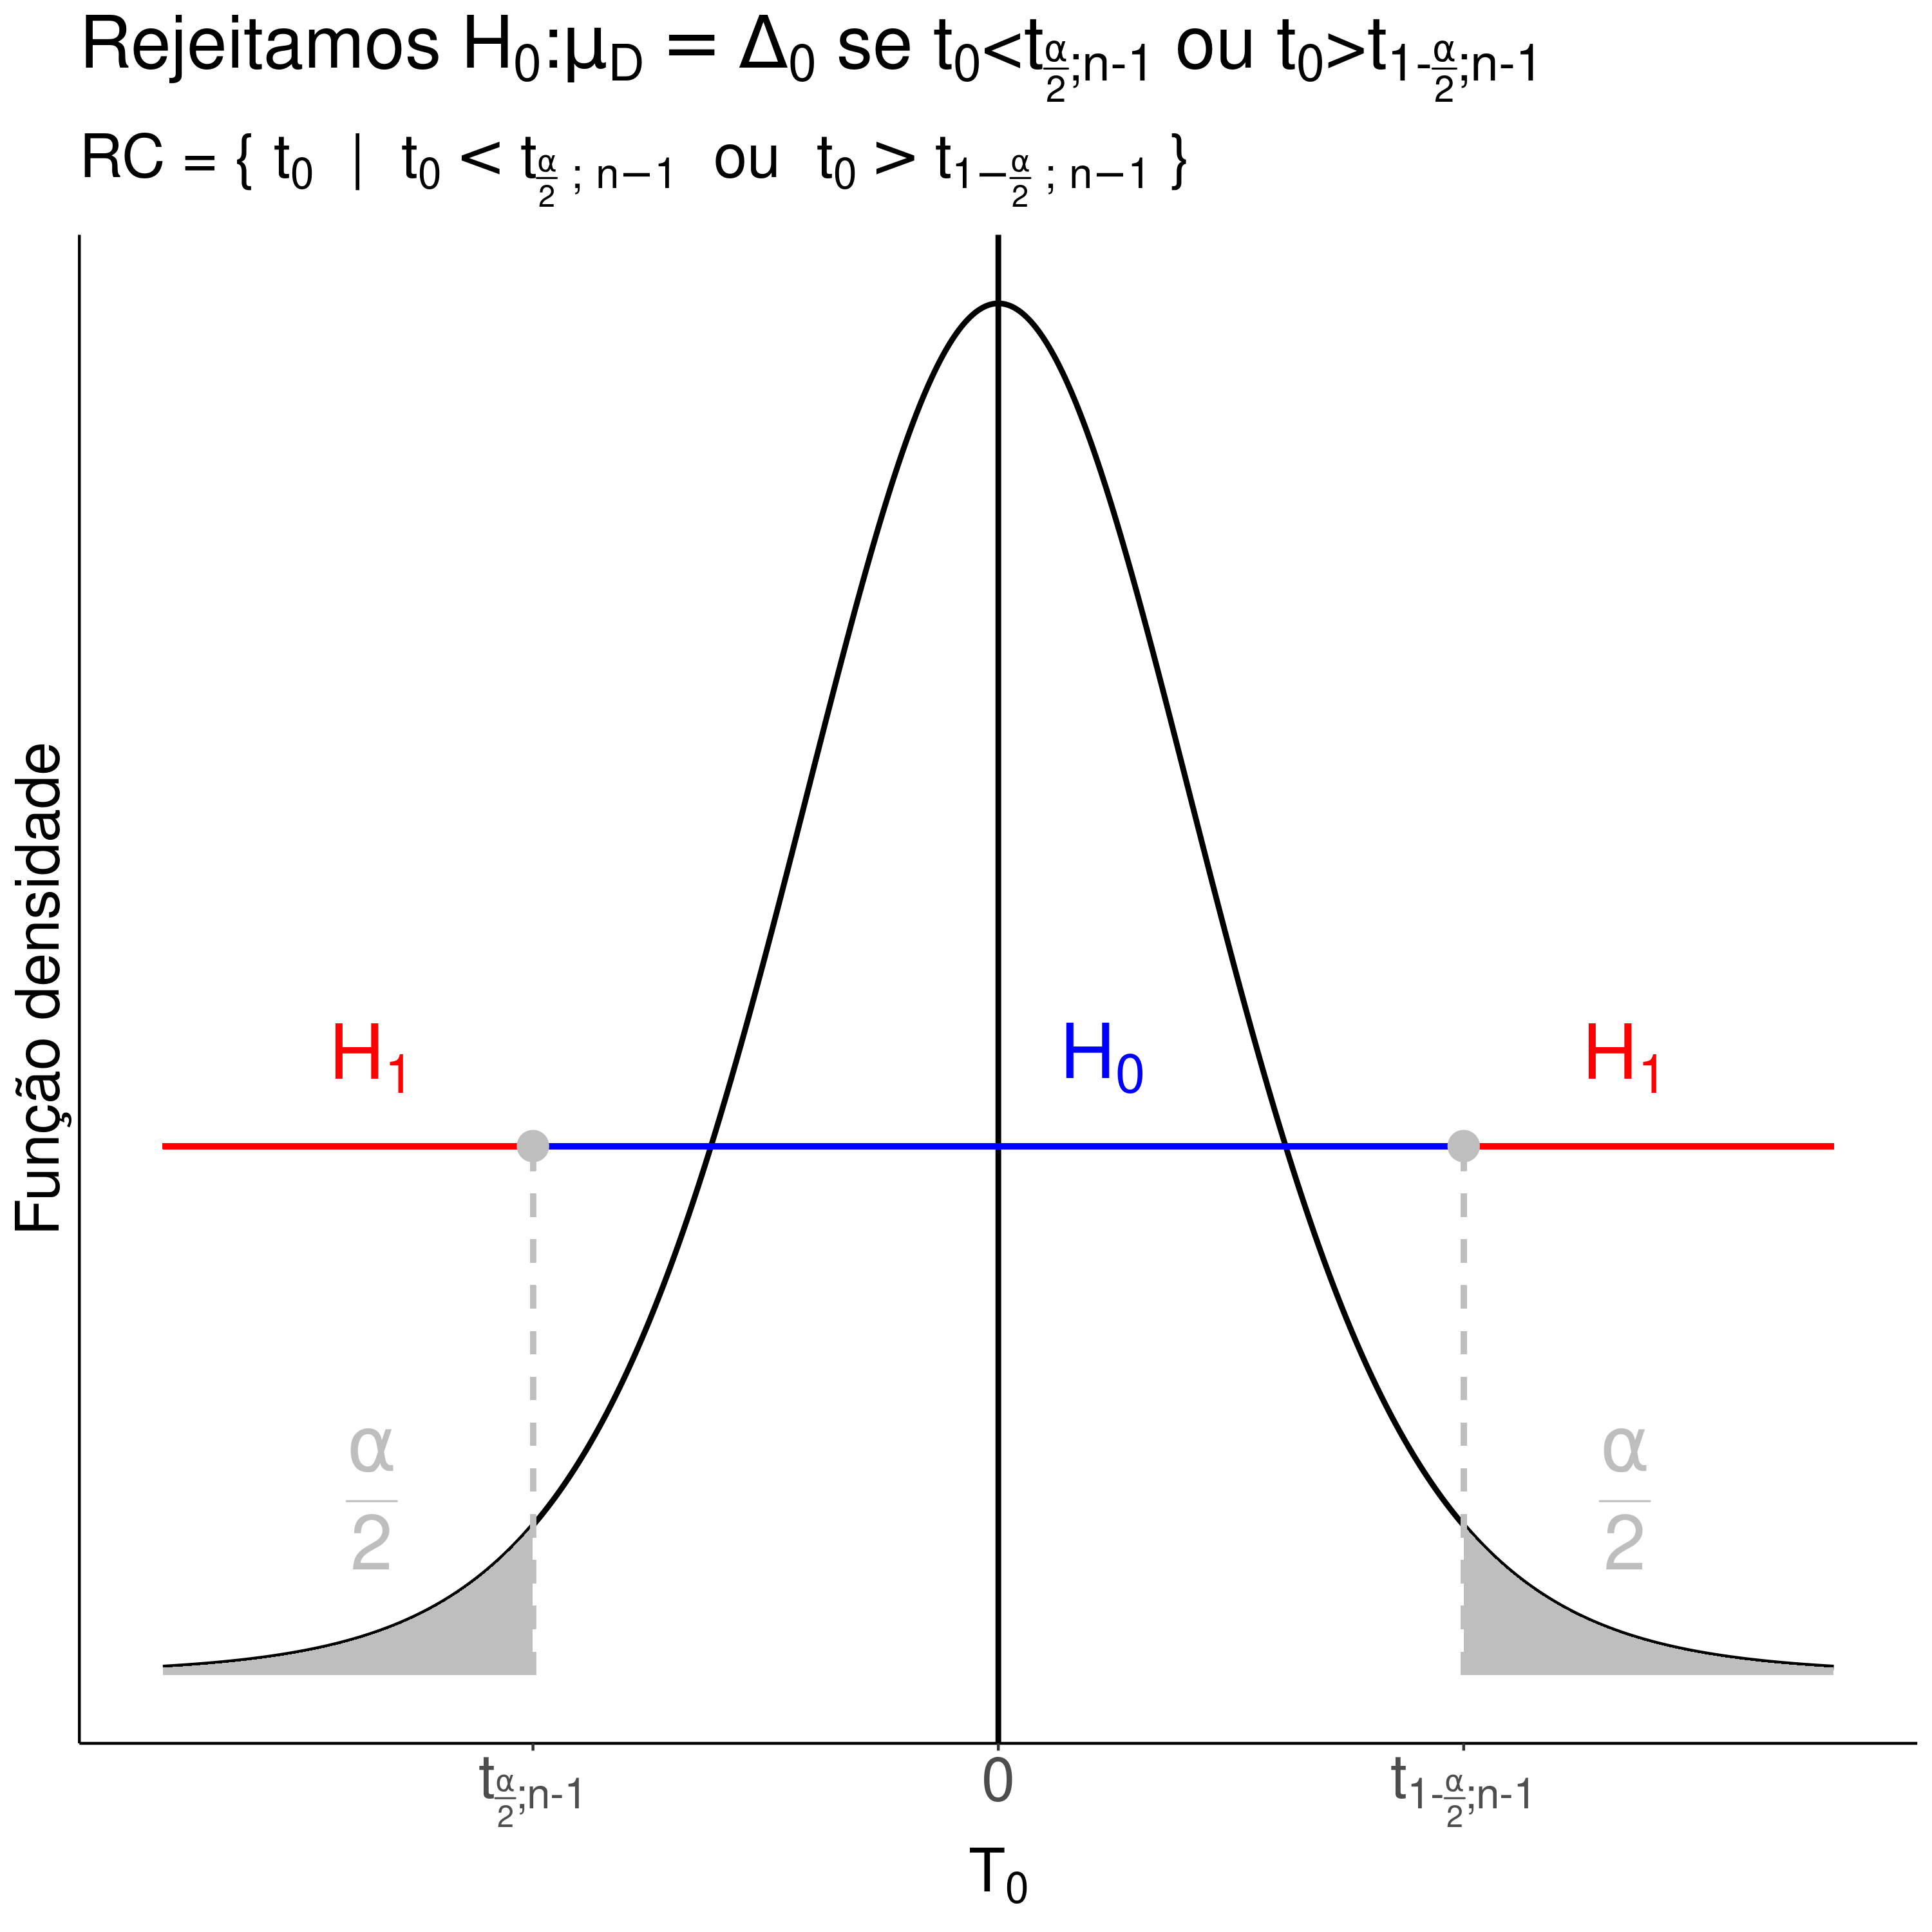
\includegraphics[width=0.32\linewidth]{figures/paired-t-test-bilateral.png} \label{fig:paired-t-test-bilateral}} \hfill
	\subfloat[][Teste bilateral.]{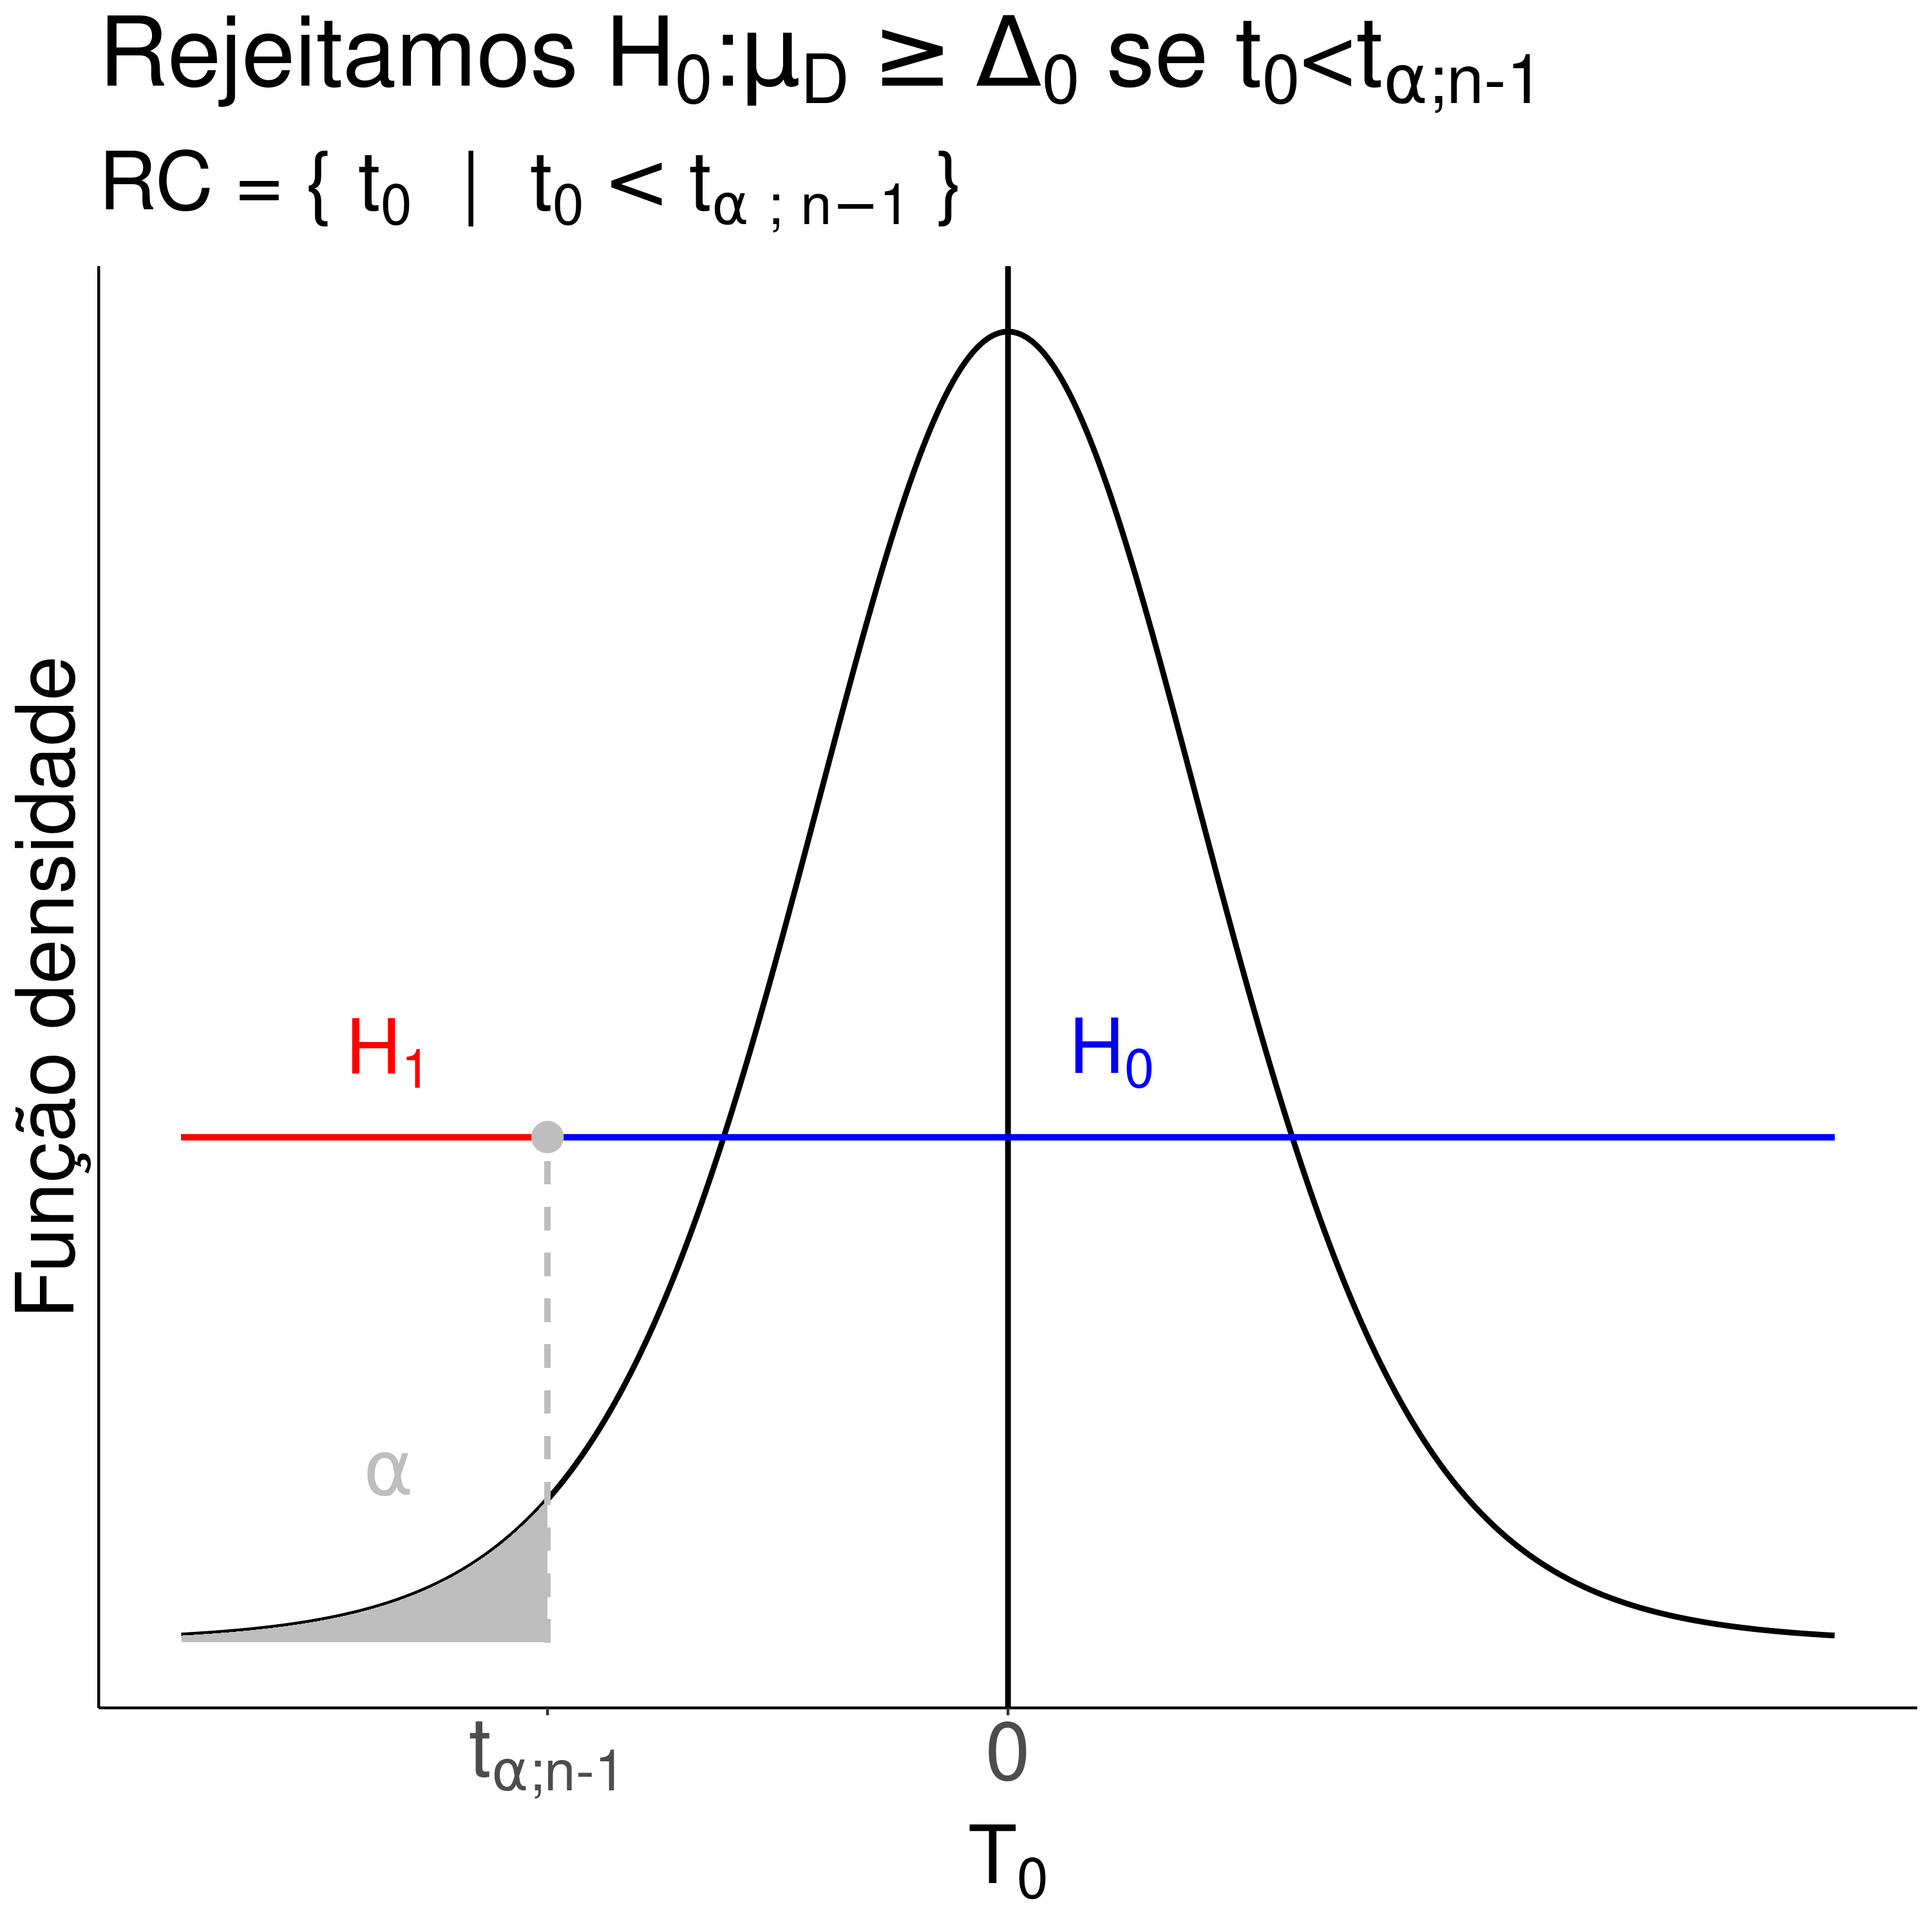
\includegraphics[width=0.32\linewidth]{figures/paired-t-test-h1-lower.png} \label{fig:paired-t-test-h1-lower}} \hfill
	\subfloat[][Teste bilateral.]{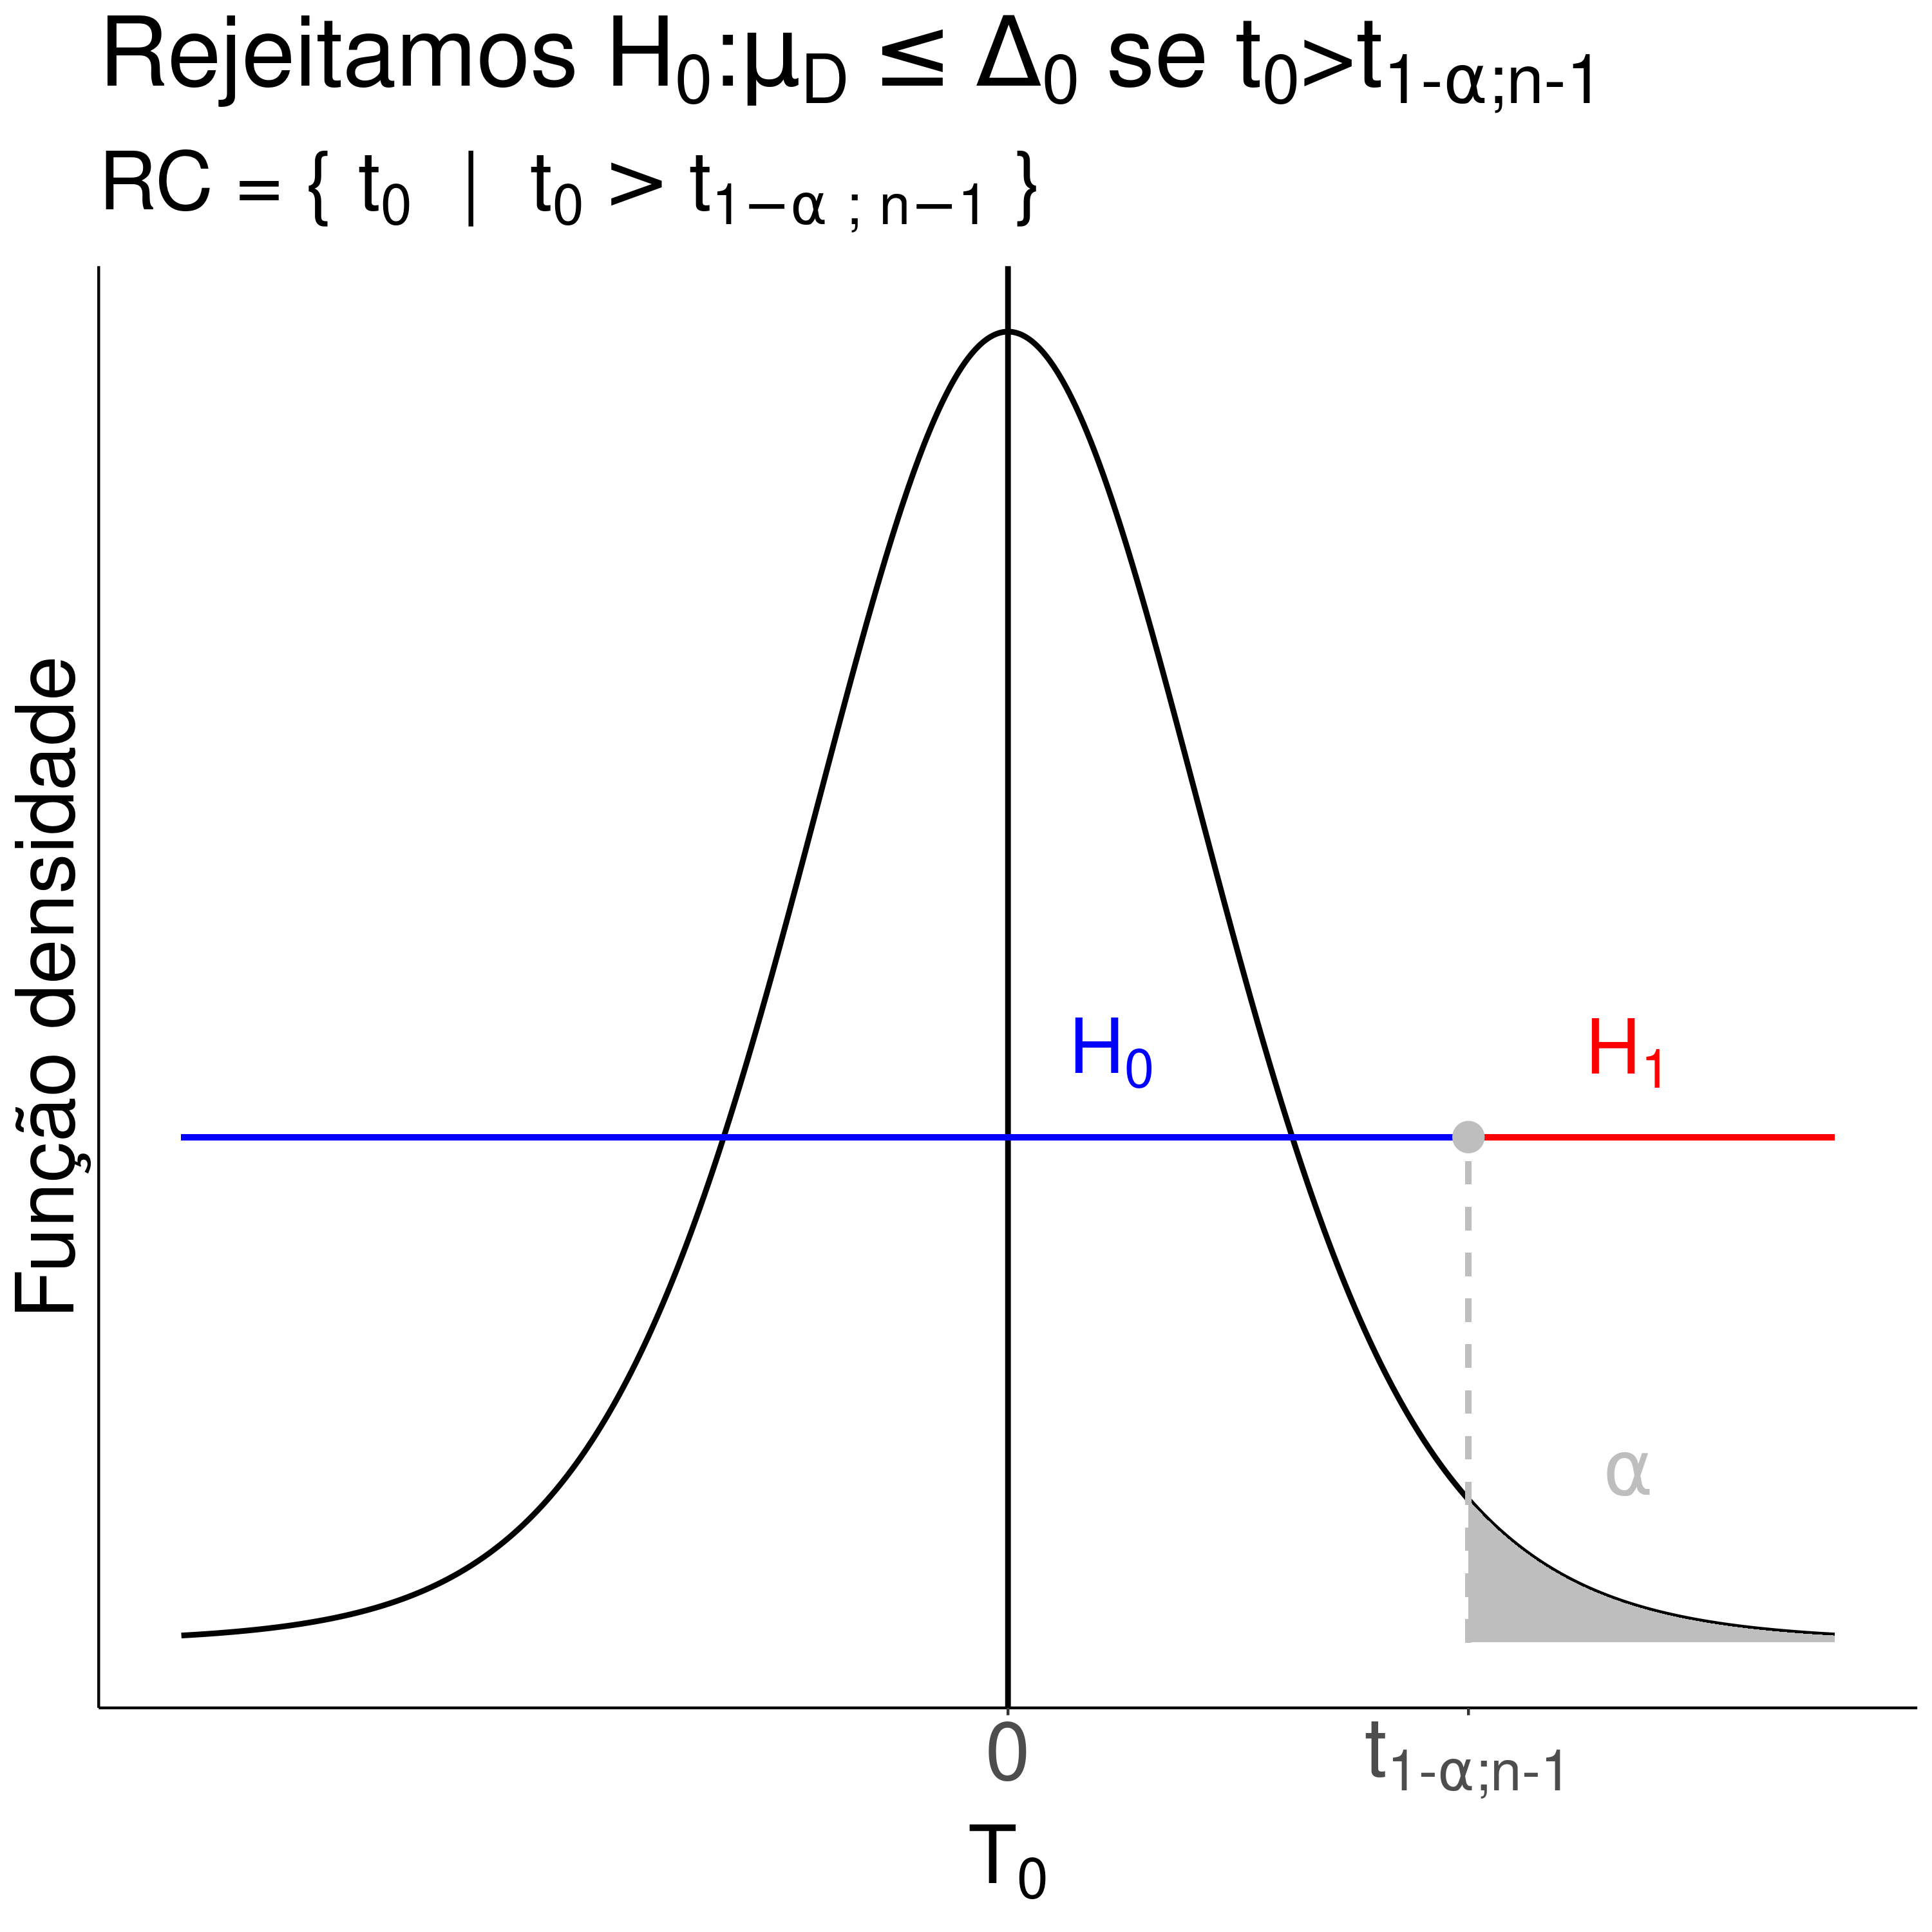
\includegraphics[width=0.32\linewidth]{figures/paired-t-test-h1-upper.png} \label{fig:paired-t-test-h1-upper}} 
	\caption{Região crítica para o teste-t pareado.}
\end{figure}
\end{frame}

\begin{frame}{Test t pareado para $\mu_D = \mu_1 - \mu_2$}

\normalsize

\begin{itemize}
	\item Na Figura~\ref{fig:paired-t-test-bilateral}, testamos $H_0: \mu_D = \Delta_0$ versus $H_1: \mu_D \neq \Delta_0$. Rejeitamos $H_0$ se $t_0 = \frac{(\bar{D} - \Delta_0)\sqrt{n}}{ s_D } \in  RC=\{t_0 \mid t_0 < t_{\frac{\alpha}{2};n-1} \allowbreak \mbox{ ou } t_0 > t_{1-\frac{\alpha}{2};n-1} \}$, em que $P\left(t_{n-1} \leq t_{\frac{\alpha}{2}; n-1} \right) = \frac{\alpha}{2}$, $P\left(t_{n-1} \leq t_{1-\frac{\alpha}{2}; n-1} \right) = 1 - \frac{\alpha}{2}$, $S_D = \frac{\sum_{k=1}^{n}(d_j - \bar{D})^2}{n-1}$, $d_j = x_{1j} - x_{2j}, j=1, \dots, n$ e $\bar{D} = \bar{X}_1 - \bar{X}_2$;
	\vfill
	
	\item Na Figura~\ref{fig:paired-t-test-h1-lower}, testamos $H_0: \mu_D \leq \Delta_0 $ versus $H_1: \mu_D > 0$. Rejeitamos $H_0$ se $t_0 = \frac{(\bar{D} - \Delta_0)\sqrt{n}}{ s_D } \in \allowbreak RC=\{t_0 \mid t_0 > t_{1-\alpha; n-1}  \}$, em que $P\left(t_{n-1} \leq  t_{1-\alpha;n-1} \right) =1- \alpha$, $S_D = \frac{\sum_{k=1}^{n}(d_j - \bar{D})^2}{n-1}$, $d_j = x_{1j} - x_{2j}, j=1, \dots, n$ e $\bar{D} = \bar{X}_1 - \bar{X}_2$;
	\vfill
	
	\item Na Figura~\ref{fig:paired-t-test-h1-upper}, testamos $H_0: \mu_D \geq \Delta_0$ versus $H_1: \mu_D  < 0$. Rejeitamos $H_0$ se $t_0 = \frac{(\bar{D} - \Delta_0)\sqrt{n}}{ s_D } \in \allowbreak RC=\{t_0 \mid t_0 < t_{\alpha;n-1}  \}$, em que $P\left(t_{n-1} \leq  t_{1-\alpha;n-1} \right) =1- \alpha$, $S_D = \frac{\sum_{k=1}^{n}(d_j - \bar{D})^2}{n-1}$, $d_j = x_{1j} - x_{2j}, j=1, \dots, n$ e $\bar{D} = \bar{X}_1 - \bar{X}_2$.
\end{itemize}
$t_{\alpha;n-1}$, $t_{1-\alpha;n-1}$, $t_{\frac{\alpha}{2};n-1}$ e $t_{1-\frac{\alpha}{2};n-1}$ são chamados de valores críticos. 

\normalsize

\end{frame}


\begin{frame}{Test t pareado para $\mu_D = \mu_1 - \mu_2$}

\begin{block}{Exemplo}
	Um pesquisador deseja comparar dois métodos para predizer a resistência ao cisalhamento das vigas de chapa de aço. Dados dos dois métodos, o procedimento de Karlsruhe e o procedimento de Lehigh, quando aplicados a nove vigas de chapa de aço são mostradas na Tabela~\ref{tab:paired-t-test-bilateral}. Existe diferença entre os dois métodos? Use $\alpha=5\%$. Calcule o valor-p.
\end{block}

\begin{table}[ht]
	\centering
	\scalebox{0.85}{
	\begin{tabular}{l|cc|c}
		\toprule[0.05cm]
		Vigas & Método Karlsruhe & Método Lehigh & Diferença $d$ \\ 
		\midrule[0.025cm]
			Vigas 1 & 1,19 & 1,06 & 0,12 \\ 
			Vigas 2 & 1,15 & 0,99 & 0,16 \\ 
			Vigas 3 & 1,32 & 1,06 & 0,26 \\ 
			Vigas 4 & 1,34 & 1,06 & 0,28 \\ 
			Vigas 5 & 1,20 & 1,06 & 0,14 \\ 
			Vigas 6 & 1,40 & 1,18 & 0,22 \\ 
			Vigas 7 & 1,36 & 1,04 & 0,33 \\ 
			Vigas 8 & 1,54 & 1,09 & 0,45 \\ 
			Vigas 9 & 1,56 & 1,05 & 0,51 \\ 
		\bottomrule[0.05cm]
	\end{tabular}
	}
	\caption{Previsões de resistência para nove vigas de chapa de aço.} 
	\label{tab:paired-t-test-bilateral}
\end{table}

\end{frame}

\begin{frame}{Test t pareado para $\mu_D = \mu_1 - \mu_2$}

\begin{block}{Solução}
	Considere a média populacional  $\mu_1$ do cisalhamento do método Karlsruhe e a média populacional $\mu_2$ do método Lehigh.
	
	\textbf{Passo 1)} Queremos testar as hipóteses: $H_0: \mu_D = \Delta_0= 0$ e $H_1: \mu_D \neq \Delta_0= 0$;
	
	\textbf{Passo 2)} Nível de significância $\alpha=5\%$;
	
	\textbf{Passo 3)} Rejeitamos $H_0$ se $t_0 = \frac{(\bar{D} - \Delta_0) \sqrt{n}}{s_D}$, em que $\bar{D} = \bar{X}_1 - \bar{X}_2$. Ou seja, $RC = \left\{ t_0 \mid t_0 < t_{\frac{\alpha}{2}; n-1} \mbox{ ou } t_0 < t_{1-\frac{\alpha}{2}; n-1} \right\}$;
	
	\textbf{Passo 4)} Vamos encontrar os valores críticos:
	\begin{itemize}
		\item $P(t_{n-1} \leq t_{1-\frac{\alpha}{2}; n-1}) = P(t_{8} \leq t_{0,975; 8}) = 0,975$, então $t_{0,975; 8} = 2,306$;
		\item $P(t_{n-1} \leq t_{\frac{\alpha}{2}; n-1}) = P(t_{8} \leq t_{0,025; 8}) = 0,025$, então $t_{0,025; 8} = -2,306$.
	\end{itemize}

	\textbf{Passo 5)} Note que $\bar{d} = 0,274$, $n=8$, $s_D = 0,135$, $\Delta_0=0$ e $t_0 = \frac{(\bar{d} - \Delta_0)\sqrt{n}}{s_D} = \frac{(0,274 - 0)\sqrt{8}}{0,135} = 6,08$. Como $t_0 \in RC$ e rejeitamos $H_0$, e as previsões dos dois métodos são distintos.
\end{block}

\end{frame}

\begin{frame}{Test t pareado para $\mu_D = \mu_1 - \mu_2$}

\begin{block}{Solução (valor-p)}
	O valor-p é calculado através de
	\begin{align*}
		p = P \left( \lvert T_0 \rvert > \lvert t_0 \rvert \mid H_0 \right) = 2 \cdot \left[1 - P \left( t_{n-1}  \leq \lvert t_0 \rvert  \right)\right].
	\end{align*}
	
	Como $n=8$, $s_D = 0,135$, $\Delta_0 = 0$, $\bar{d} = 0,274$ e $t_0 = 6,08$, então
	\begin{align*}
		p &=2 \cdot \left[1 - P \left(t_{n-1} \leq  \lvert t_0 \rvert \right)\right]\\
		&= 2 \cdot \left[1 - P \left(t_{8} \leq   6,08  \right)\right]\\
		&= 0,0003.
	\end{align*}
	
	Como $p=0,0003 < \alpha = 0,05$, então rejeitamos $H_0$ ao nível de significância $\alpha=0,05$. Ou seja, ao nível de significância $\alpha=5\%$, os métodos de previsão são diferentes.
\end{block}

\end{frame}

\begin{frame}{Test t pareado para $\mu_D = \mu_1 - \mu_2$}
	\begin{block}{Exemplo}
		Quinze homens adultos entre 35 e 50 anos participaram em um estudo para avaliar os efeito da dieta e exercício físico no nível de colesterol no sangue. Inicialmente mediu-se o nível de colesterol. Três meses depois de participação do estudo em que fizeram exercícios aeróbicos e uma dieta de baixa gordura,  mediu-se novamente o nível de colesterol. Os dados estão na Tabela~\ref{tab:col}. Ao nível de significância $5\%$, o nível médio de colesterol diminuiu? Calcule o valor-p.
	\end{block}

\begin{table}[ht]
	\centering
	\scalebox{0.5}{
	\begin{tabular}{l|cc}
		\toprule[0.05cm]
		Sujeito & Antes & Depois \\ 
		\midrule[0.025cm]
		Sujeito 1 & 265 & 229 \\ 
		Sujeito 2 & 240 & 231 \\ 
		Sujeito 3 & 258 & 227 \\ 
		Sujeito 4 & 295 & 240 \\ 
		Sujeito 5 & 251 & 238 \\ 
		Sujeito 6 & 245 & 241 \\ 
		Sujeito 7 & 287 & 234 \\ 
		Sujeito 8 & 314 & 256 \\ 
		Sujeito 9 & 260 & 247 \\ 
		Sujeito 10 & 279 & 239 \\ 
		Sujeito 11 & 283 & 246 \\ 
		Sujeito 12 & 240 & 218 \\ 
		Sujeito 13 & 238 & 219 \\ 
		Sujeito 14 & 225 & 226 \\ 
		Sujeito 15 & 247 & 233 \\ 
		\bottomrule[0.05cm]
	\end{tabular}
	}
	\caption{Nível de colesterol.} 
	\label{tab:col}
\end{table}
\end{frame}

\begin{frame}{Test t pareado para $\mu_D = \mu_1 - \mu_2$}

\begin{block}{Solução}
	Considere $\mu_1$ o nível de colesterol antes do estudo começar e $\mu_2$ o nível de colesterol depois do estudo finalizado.
	
	\textbf{Passo 1)} Queremos testar as hipóteses: $H_0: \mu_D = \mu_1 - \mu_2 \leq \Delta_0=0$ e $H_1:\mu_D = \mu_1 - \mu_2 > \Delta_0 = 0$;
	
	\textbf{Passo 2)} Nível de significância $\alpha=5\%$;
	
	\textbf{Passo 3)} Rejeitamos $H_0$ se $t_0 = \frac{(\bar{D} - \Delta_0)\sqrt{n}}{s_D}$, em que $\bar{D} = \bar{X}_1 - \bar{X}_2$. Ou seja, $RC= \left\{ t_0 \mid t_0 > t_{1-\alpha; n-1}  \right\}$;
	
	\textbf{Passo 4)} Vamos encontrar valor crítico:
	\begin{itemize}
		\item $P\left(t_{n-1} \leq t_{1-\alpha;n-1}\right) = P\left(t_{14} \leq t_{0,95;14}\right) = 1-\alpha = 0,95$, então $t_{0,95;14} = 1,761$.
	\end{itemize}

	\textbf{Passo 5)} Como $\bar{d} = 26,87$, $s_D = 19,04$, $n=15$ e $t_0 = 5,47$. Então $t_0 \in RC$ e rejeitamos $H_0$. Ou seja, ao nível de significância $5\%$, o nível colesterol diminuiu depois de três meses de dieta com baixa gordura e exercícios físicos.
\end{block}

\end{frame}

\begin{frame}{Test t pareado para $\mu_D = \mu_1 - \mu_2$}

\begin{block}{Solução (valor-p)}
	O valor-p pode ser calculado por
	\begin{align*}
		p &= P \left( T_0 > t_0 \mid H_0 \right) = 1 - P(t_{n-1} \leq t_0).
	\end{align*}	
	
	Como $n = 15$, $\bar{D} = 26,87$, $s_D = 19,04$ e $t_0=5, 47$, então o valor-p é dado por
	\begin{align*}
		p &= 1 - P\left( t_{n-1} \leq t_0 \right)\\
		&= 1 - P \left( t_{14} \leq 5,47 \right)\\
		&= 0,00004.
	\end{align*}
	
	Como $p = 0,00004 < \alpha = 0,05$, rejeitamos $H_0$. Ou seja, ao nível de significância $\alpha=5\%$, o nível médio de colesterol depois de três meses com dieta de baixa gordura e exercícios físicos diminuiu.
\end{block}

\end{frame}

\begin{frame}{Test t pareado para $\mu_D = \mu_1 - \mu_2$}

\begin{block}{Exemplo}
	Considere um estudo observacional completamente aleatório para estudar $\mu_D = \mu_1 - \mu_2$, em que a população 1 tem distribuição normal com média populacional $\mu_1$ e a população 2 tem distribuição normal com média populacional $\mu_2$. Suponha que o pesquisador deseja decidir entre as hipóteses $H_0:\mu_D = \mu_1 - \mu_2 \geq \Delta_0$ e $H_1: \mu_D = \mu_1 - \mu_2 < \Delta_0$. Na Tabela~\ref{tab:test-t-pareado-h1-upper} temos algumas informações sobre o experimento. Complete a Tabela~\ref{tab:test-t-pareado-h1-upper}. Qual a decisão do pesquisador? Use $\alpha = 5\%$.
	
	\begin{table}[htbp]
		\centering
		\begin{tabular}{c|c|c|c}
			\toprule[0.05cm]
			$\bar{x}_1$ & $\bar{x}_2$ & $\alpha$ & $t_0$ \\ \midrule[0.025cm]
			$15,43$ & $20,58$ & $5\%$ &  \\ \midrule[0.05cm]
			$\Delta_0$ & $n$ & valor-p & $s_D$ \\ \midrule[0.025cm]
			$0$ & $20$ &  & $0,43$ \\ \bottomrule[0.05cm]
		\end{tabular}
		\caption{Algumas informações do experimento.}
		\label{tab:test-t-pareado-h1-upper}
	\end{table}
\end{block}

\end{frame}

\begin{frame}{Test t pareado para $\mu_D = \mu_1 - \mu_2$}

\begin{block}{Exemplo}
	\textbf{Passo 1)} Queremos testar as hipóteses: $H_0: \mu_D \geq \Delta_0 = 0$ e $H_0: \mu_D < \Delta_0 = 0$;
	
	\textbf{Passo 2)} Nível de significância $\alpha=5\%$;
	
	\textbf{Passo 3)} Rejeitamos $H_0$ se $t_0 = \frac{(\bar{D} - \Delta_0)\sqrt{n}}{s_D}$ for pequeno. Ou seja, $RC = \left\{ t_0 \mid t_0 < t_{\alpha; n-1} \right\}$;
	
	\textbf{Passo 4)} Vamos encontrar o valor crítico:
	\begin{itemize}
		\item $P(t_{n-1} \leq t_{\alpha; n-1}) = P(t_{19} \leq t_{0,05; 19}) = \alpha = 0,05$, então $t_{0,05; 19} = -1,729$;
	\end{itemize}

	\textbf{Passo 5)} Note que $\bar{d} = \bar{x}_1 - \bar{x}_2 = 15,43 - 20,58 = -5,15$ e $t_0 = \frac{(\bar{D} - \Delta_0)\sqrt{n}}{s_D} = \frac{(-5,15 - 0)\sqrt{20}}{0,43} = -53,56 \in RC$, então rejeitamos $H_0$.
\end{block}

\end{frame}

\begin{frame}{Test t pareado para $\mu_D = \mu_1 - \mu_2$}

\begin{block}{Solução (valor-p)}
	O valor-p é dado por
	$$p = P(T_0 < t_0 \mid H_0) = P(t_{n-1} \leq t_0).$$
	
	Note que $\bar{d} = \bar{x}_1 - \bar{x}_2 = 15,43 - 20,58 = -5,15$ e $t_0 = \frac{(\bar{D} - \Delta_0)\sqrt{n}}{s_D} = \frac{(-5,15 - 0)\sqrt{20}}{0,43} = -53,56$. Então, o valor-p é dado por
	\begin{align*}
	p &= P(t_{n-1} \leq t_0)\\
	&= P(t_{19} \leq -53,56)\\
	&= 0.
	\end{align*}
	
	Como $p=0 < \alpha = 0,05$, então rejeitamos $H_0$.
\end{block}

\end{frame}

\subsection{Poder e tamanho da amostra.}

\begin{frame}{Poder do teste: $H_0:\mu_D = \mu_1 - \mu_2 = \Delta_0$ e $H_1:\mu_D =  \mu_1 - \mu_2 \neq \Delta_0$.}

\footnotesize

Imagine que
\begin{itemize}
	\item Hipóteses: $H_0:\mu_D= \mu_1 - \mu_2 = \Delta_0$ e $H_1:\mu_D= \mu_1 -  \mu_2 \neq \Delta_0$;
	\item $H_1$ é verdade, então $\mu_D = \mu_1-\mu_2 \neq \Delta_0$ e seja $\sigma_D$ é a variância populacional de $X_1 - X_2$;
	\item $T_0 = \frac{(\bar{D} - \Delta_0) \sqrt{n}}{s_D} \sim t_{n-1}\left( \frac{(\mu_D - \Delta_0)\sqrt{n}}{\sigma_D} \right)$;
	\item Ao nível de significância $\alpha$, temos $RC = \left\{ t_0 \mid t_0 < t_{\frac{\alpha}{2};n-1} \mbox{ ou } t_0 < t_{1-\frac{\alpha}{2}; n-1} \right\}$.
\end{itemize}
\vfill	

Poder do teste é dado
\begin{align*}
\textcolor{important}{1-\beta} &=1 - \left[P\left( t_{\frac{\alpha}{2};n-1} \leq T_0 \leq t_{1-\frac{\alpha}{2};n-1}  \mid H_1 \right)\right]\\
&= 1 - \left[P\left( T_0 \leq t_{1-\frac{\alpha}{2};n-1} \mid \mu_D \neq \Delta_0 \right) - P\left( T_0 \leq t_{\frac{\alpha}{2};n-1} \mid \mu_D \neq \Delta_0 \right) \right]\\ 
&= \textcolor{important}{1 - P\left( t_{n-1}\left( \frac{(\mu_D - \Delta_0)\sqrt{n}}{\sigma_D} \right) \leq t_{1-\frac{\alpha}{2};n-1} \right) + P\left( t_{n-1}\left( \frac{(\mu_D - \Delta_0)\sqrt{n}}{\sigma_D} \right) \leq t_{\frac{\alpha}{2};n-1} \right).}
\end{align*}
A \textcolor{important}{Função Poder}, dado o tamanho da amostra $n$, é uma função das médias populacionais na hipótese alternativa  $\pi: \mathbb{R} -\{\Delta_0\} \longrightarrow [0,1]$ dada por
\begin{align*}
\pi(\mu_D) = 1 - P\left( t_{n-1}\left( \frac{(\mu_D - \Delta_0)\sqrt{n}}{\sigma_D} \right) \leq t_{1-\frac{\alpha}{2};n-1} \right) + P\left( t_{n-1}\left( \frac{(\mu_D - \Delta_0)\sqrt{n}}{\sigma_D} \right) \leq t_{\frac{\alpha}{2};n-1} \right),
\end{align*}
em que $ \mu_D \in \mathbb{R} - \{\Delta_0\}.$ Alguns livros chamam a Função Poder de \textcolor{important}{Curva de Característica Operacional.}

\normalsize

\end{frame}


\begin{frame}[fragile]{Tamanho da amostra: $H_0:\mu_1 - \mu_2 = \Delta_0$ e $H_1: \mu_1 - \mu_2 \neq \Delta_0$.}

\scriptsize
Imagine que
\begin{itemize}
	\item Hipóteses: $H_0:\mu_D= \mu_1 - \mu_2 = \Delta_0$ e $H_1:\mu_D= \mu_1 -  \mu_2 \neq \Delta_0$;
	\item $H_1$ é verdade, então $\mu_D = \mu_1-\mu_2 \neq \Delta_0$ e seja $\sigma_D$ é a variância populacional de $X_1 - X_2$;
	\item $T_0 = \frac{(\bar{D} - \Delta_0)\sqrt{n}}{s_D} \sim t_{n-1}\left( \frac{(\mu_D - \Delta_0)\sqrt{n}}{\sigma_D} \right)$;
	\item Ao nível de significância $\alpha$, temos $RC = \left\{ t_0 \mid t_0 < t_{\frac{\alpha}{2};n-1} \mbox{ ou } t_0 < t_{1-\frac{\alpha}{2}; n-1} \right\}$.
\end{itemize}
\vfill

Considere $1-\beta$, $\alpha$, $n_1=n_2=n$, então o tamanho \sout{mínimo} da amostra é solução da seguinte equação
\scriptsize
\begin{align}\label{eq:pwr-paired-t-test-bilateral}
1-\beta = 1 - P\left( t_{n-1}\left( \frac{(\mu_D - \Delta_0)\sqrt{n}}{\sigma_D} \right) \leq t_{1-\frac{\alpha}{2};n-1} \right) + P\left( t_{n-1}\left( \frac{(\mu_D - \Delta_0)\sqrt{n}}{\sigma_D} \right) \leq t_{\frac{\alpha}{2};n-1} \right).
\end{align}
\normalsize

A equação~\eqref{eq:pwr-paired-t-test-bilateral} é resolvida usando métodos numéricos que estão implementados em diversos \textit{softwares}.
\begin{description}
	\item[No R] \lstinline|pwr_paired_t_test|
\end{description}
Esta função está no pacote \lstinline|power|, que pode ser instalado usando o pacote \lstinline|devtools|: \lstinline|devtools::install_github("gilberto-sassi/power")|.


\end{frame}

\begin{frame}{Poder do teste: $H_0:\mu_D = \mu_1 - \mu_2 = \Delta_0$ e $H_1:\mu_D =  \mu_1 - \mu_2 \neq \Delta_0$.}

\large
\begin{block}{Exemplo}
	Um pesquisador deseja comparar dois métodos para predizer a resistência ao cisalhamento das vigas de chapa de aço. Existem dois métodos, o procedimento de Karlsruhe e o procedimento de Lehigh, e o pesquisador planeja usar nove vigas para prever o cisalhamento usando os dois métodos. Imagine que a diferença das médias populações é $\mu_D = \mu_{\tiny Karlsruhe} - \mu_{\tiny Lehigh} = 0,3$ e o desvio padrão da diferença de cisalhamento é $\sigma_D = 0,5$. Qual o poder do teste? Use $\alpha=5\%$. 
\end{block}	
\normalsize

\end{frame}

\begin{frame}[fragile]{Poder do teste: $H_0:\mu_D = \mu_1 - \mu_2 = \Delta_0$ e $H_1:\mu_D =  \mu_1 - \mu_2 \neq \Delta_0$.}

\footnotesize
\begin{block}{Solução}
	Considere $\mu_1=\mu_{\tiny Karlsruhe}$ é a média do ponto de cisalhamento para o procedimento de Karlsruhe e $\mu_2 = \mu_{\tiny Lehigh}$ é a média do ponto de cisalhamento para o procedimento de Lehigh. Então $\mu_D = \mu_1 - \mu_2$.
	
	\textbf{Passo 1)} Queremos testar as hipótese: $H_0: \mu_D = \Delta_0 = 0$ e $H_1: \mu_D \neq \Delta_0 = 0$;
	
	\textbf{Passo 2)} Nível de significância $\alpha=5\%$;
	
	Note que $\mu_D = 0,3$, $\sigma_D = 0,1$, $n=9$, $\Delta_0=0$, $\alpha=5\%$, $\mu =  \frac{( \mu_D - \Delta_0)\sqrt{n}}{\sigma_D} =9$.
	
	Primeiro calculamos os quantis de distribuição normal padrão:
	\begin{itemize}
		\item $P\left( t_{n-1} \leq t_{1-\frac{\alpha}{2}; n-1} \right) = P\left( t_{8} \leq t_{0,975; 8} \right) = 1-\frac{\alpha}{2} = 0,975$, então $t_{0,975; 8} = 2,306$;
		\item $P\left( t_{n-1} \leq t_{1-\frac{\alpha}{2}; n-1} \right) = P\left( t_{8} \leq t_{0,025; 8} \right) = \frac{\alpha}{2} = 0,025$, então $t_{0,025; 8} = -2,306$.
	\end{itemize}

	Então, o poder de teste é dado por
	\begin{align*}
	1-\beta &= 1 - P\left( t_{n-1}\left( \frac{(\mu_D - \Delta_0)\sqrt{n}}{\sigma_D} \right) \leq t_{1-\frac{\alpha}{2};n-1} \right) + P\left( t_{n-1}\left( \frac{(\mu_D - \Delta_0)\sqrt{n}}{\sigma_D} \right) \leq t_{\frac{\alpha}{2};n-1} \right)\\
	&= 1 - P \left( t_8 (9) \leq 2,306 \right) + P \left( t_8 (9) \leq -2,306 \right) =1.
	\end{align*}
\end{block}

\begin{lstlisting}[language = C, caption = Código no R.]
pwr_paired_t_test(sigma_d = 0.1, delta = 0.3, delta0 = 0, n = 9,
		pwr = NULL, alternative = "two.sided", sig_level = 0.05)
\end{lstlisting}

\normalsize

\end{frame}

\begin{frame}{Tamanho do teste: $H_0:\mu_D = \mu_1 - \mu_2 = \Delta_0$ e $H_1:\mu_D =  \mu_1 - \mu_2 \neq \Delta_0$.}

\large
\begin{block}{Exemplo}
	Um pesquisador deseja comparar dois métodos para predizer a resistência ao cisalhamento das vigas de chapa de aço. Existem dois métodos, o procedimento de Karlsruhe e o procedimento de Lehigh, e o pesquisador planeja usar vigas para prever o cisalhamento usando os dois métodos. Imagine que a diferença das médias populações é $\mu_D = \mu_{\tiny Karlsruhe} - \mu_{\tiny Lehigh} = 0,3$ e o desvio padrão da diferença de cisalhamento é $\sigma_D = 0,5$. Com poder do teste $99\%$, quantas vigas de aço precisamos analisar? Use $\alpha=5\%$. 
\end{block}	
\normalsize

\end{frame}

\begin{frame}[fragile]{Tamanho do teste: $H_0:\mu_D = \mu_1 - \mu_2 = \Delta_0$ e $H_1:\mu_D =  \mu_1 - \mu_2 \neq \Delta_0$.}

\begin{block}{Solução}
Considere $\mu_1=\mu_{\tiny Karlsruhe}$ é a média do ponto de cisalhamento para o procedimento de Karlsruhe e $\mu_2 = \mu_{\tiny Lehigh}$ é a média do ponto de cisalhamento para o procedimento de Lehigh. Então $\mu_D = \mu_1 - \mu_2$.

\textbf{Passo 1)} Queremos testar as hipótese: $H_0: \mu_D = \Delta_0 = 0$ e $H_1: \mu_D \neq \Delta_0 = 0$;

\textbf{Passo 2)} Nível de significância $\alpha=5\%$;

Como $\mu_D = 0,3$, $\sigma_D = 0,5$, $1-\beta=0,99$, $\alpha=5\%$, $\Delta_0=0$, então o tamanho \sout{mínimo} da amostra é solução da seguinte equação
{\scriptsize
\begin{align*}
1-\beta &= 0,99= 1 - P\left( t_{n-1}\left( \frac{(\mu_D - \Delta_0)\sqrt{n}}{\sigma_D} \right) \leq t_{1-\frac{\alpha}{2};n-1} \right) + P\left( t_{n-1}\left( \frac{(\mu_D - \Delta_0)\sqrt{n}}{\sigma_D} \right) \leq t_{\frac{\alpha}{2};n-1} \right)\\
&= 1 - P\left( t_{n-1}\left( \frac{(0,3)\sqrt{n}}{0,5} \right) \leq t_{0,975;n-1} \right) + P\left( t_{n-1}\left( \frac{(0,3)\sqrt{n}}{0,5} \right) \leq t_{0,025;n-1} \right)
\end{align*}
}

Então, este pesquisador precisa analisar $n=54$ vigas de aço.
\end{block}

\begin{lstlisting}[language = C, caption = Código no R.]
pwr_paired_t_test(sigma_d = 0.5, delta = 0.3, delta0 = 0, n = NULL,
		pwr = 0.99, alternative = "two.sided", sig_level = 0.05)
\end{lstlisting}

\end{frame}

\begin{frame}{Poder do teste: $H_0:\mu_D = \mu_1 - \mu_2 \leq \Delta_0$ e $H_1:\mu_D =  \mu_1 - \mu_2 > \Delta_0$.}

\normalsize

Imagine que
\begin{itemize}
	\item Hipóteses: $H_0:\mu_D= \mu_1 - \mu_2 \leq \Delta_0$ e $H_1:\mu_D= \mu_1 -  \mu_2 > \Delta_0$;
	\item $H_1$ é verdade, então $\mu_D = \mu_1-\mu_2 \neq \Delta_0$ e seja $\sigma_D$ é a variância populacional de $X_1 - X_2$;
	\item $T_0 = \frac{(\bar{D} - \Delta_0)\sqrt{n}}{s_D} \sim t_{n-1}\left( \frac{(\mu_D - \Delta_0)\sqrt{n}}{\sigma_D} \right)$;
	\item Ao nível de significância $\alpha$, temos $RC = \left\{ t_0 \mid t_0 > t_{1  -\alpha;n-1}  \right\}$.
\end{itemize}
\vfill	

Poder do teste é dado
\begin{align*}
\textcolor{important}{1-\beta} &=1 - \left[P\left( T_0 \leq t_{1-\alpha;n-1}  \mid H_1 \right)\right]= 1 - P\left( T_0 \leq t_{1-\alpha;n-1} \mid \mu_D \neq \Delta_0 \right) \\ 
&= \textcolor{important}{1 - P\left( t_{n-1}\left( \frac{(\mu_D - \Delta_0)\sqrt{n}}{\sigma_D} \right) \leq t_{1-\alpha;n-1} \right).}
\end{align*}
A \textcolor{important}{Função Poder}, dado o tamanho da amostra $n$, é uma função das médias populacionais na hipótese alternativa  $\pi: \mathbb{R} -\{\Delta_0\} \longrightarrow [0,1]$ dada por
\begin{align*}
\pi(\mu_D) = 1 - P\left( t_{n-1}\left( \frac{(\mu_D - \Delta_0)\sqrt{n}}{\sigma_D} \right) \leq t_{1-\alpha;n-1} \right),  \mu_D \in \mathbb{R} - \{\Delta_0\}.
\end{align*}
Alguns livros chamam a Função Poder de \textcolor{important}{Curva de Característica Operacional.}

\normalsize

\end{frame}


\begin{frame}{Tamanho da amostra: $H_0:\mu_1 - \mu_2 \leq \Delta_0$ e $H_1: \mu_1 - \mu_2 > \Delta_0$.}

\normalsize
Imagine que
\begin{itemize}
	\item Hipóteses: $H_0:\mu_D= \mu_1 - \mu_2 \leq \Delta_0$ e $H_1:\mu_D= \mu_1 -  \mu_2 > \Delta_0$;
	\item $H_1$ é verdade, então $\mu_D = \mu_1-\mu_2 \neq \Delta_0$ e seja $\sigma_D$ é a variância populacional de $X_1 - X_2$;
	\item $T_0 = \frac{(\mu_D - \Delta_0)\sqrt{n}}{s_D} \sim t_{n-1}\left( \frac{(\mu_D - \Delta_0)\sqrt{n}}{\sigma_D} \right)$;
	\item Ao nível de significância $\alpha$, temos $RC = \left\{ t_0 \mid t_0 > t_{1  -\alpha;n-1}  \right\}$.
\end{itemize}
\vfill

Considere $1-\beta$, $\alpha$, $n_1=n_2=n$, então o tamanho \sout{mínimo} da amostra é solução da seguinte equação
\scriptsize
\begin{align}\label{eq:pwr-paired-t-test-greater}
1-\beta = 1 - P\left( t_{n-1}\left( \frac{(\mu_D - \Delta_0)\sqrt{n}}{\sigma_D} \right) \leq t_{1-\alpha;n-1} \right).
\end{align}

A equação~\eqref{eq:pwr-paired-t-test-greater} é resolvida usando métodos numéricos que estão implementados em diversos \textit{softwares}.
\begin{description}
	\item[No R] \lstinline|pwr_paired_t_test|
\end{description}
Esta função está no pacote \lstinline|power|, que pode ser instalado usando o pacote \lstinline|devtools|: \lstinline|devtools::install_github("gilberto-sassi/power")|.

\normalsize
\end{frame}

\begin{frame}{Poder do teste: $H_0:\mu_D = \mu_1 - \mu_2 \leq \Delta_0$ e $H_1:\mu_D =  \mu_1 - \mu_2 > \Delta_0$.}

\large
\begin{block}{Exemplo}
	Quinze homens adultos entre 35 e 50 anos participaram em um estudo para avaliar os efeito da dieta e exercício físico no nível de colesterol no sangue. Inicialmente mediu-se o nível de colesterol. Três meses depois de participação do estudo em que fizeram exercícios aeróbicos e uma dieta de baixa gordura,  mediu-se novamente o nível de colesterol. Imagine que a média e o desvio padrão populacional são, respectivamente, $\mu_D = 25$ e $\sigma_D = 15$.  Ao nível de significância $5\%$, qual o poder do teste?
\end{block}
\normalsize

\end{frame}

\begin{frame}[fragile]{Poder do teste: $H_0:\mu_D = \mu_1 - \mu_2 \leq \Delta_0$ e $H_1:\mu_D =  \mu_1 - \mu_2 > \Delta_0$.}

\small
\begin{block}{Solução}
	Considere $\mu_1$ o nível de colesterol antes do estudo começar e $\mu_2$ o nível de colesterol depois do estudo finalizado.
	
	\textbf{Passo 1)} Queremos testar as hipóteses: $H_0: \mu_D = \mu_1 - \mu_2 \leq \Delta_0=0$ e $H_1:\mu_D = \mu_1 - \mu_2 > \Delta_0 = 0$;
	
	\textbf{Passo 2)} Nível de significância $\alpha=5\%$;
	
	Note que $\mu_D = 25$, $\sigma_D = 15$, $\Delta_0 = 0$, $\alpha=5\%$, $n=15$ e $\frac{(\mu_D - \Delta_0)\sqrt{n}}{\sigma_D} = 6,455$.
	
	Primeiro vamos calcular o quantil da distribuição $t$-Student:
	\begin{itemize}
		\item $P(t_{n-1} \leq t_{1-\alpha; n-1}) = P(t_{14} \leq t_{0,95; 14}) = 1-\alpha = 0,95$, então $t_{0,95; 14} = 1,761$.
	\end{itemize}

	Então, o poder do teste é dado por
	\begin{align*}
	1-\beta &= 1 - P\left( t_{n-1}\left( \frac{(\mu_D - \Delta_0)\sqrt{n}}{\sigma_D} \right) \leq t_{1-\alpha;n-1} \right) = 1 - P\left( t_{14}\left(6,455 \right) \leq 1,761 \right)  = 1.
	\end{align*}
\end{block}

\begin{lstlisting}[language = C, caption = Código no R.]
pwr_paired_t_test(sigma_d = 15, delta = 25, delta0 = 0, n = 15,
		pwr = NULL, alternative = "greater", sig_level = 0.05)
\end{lstlisting}

\normalsize
\end{frame}

\begin{frame}{Tamanho da amostra: $H_0:\mu_D = \mu_1 - \mu_2 \leq \Delta_0$ e $H_1:\mu_D =  \mu_1 - \mu_2 > \Delta_0$.}

\large
\begin{block}{Exemplo}
	Quinze homens adultos entre 35 e 50 anos participaram em um estudo para avaliar os efeito da dieta e exercício físico no nível de colesterol no sangue. Inicialmente mediu-se o nível de colesterol. Três meses depois de participação do estudo em que fizeram exercícios aeróbicos e uma dieta de baixa gordura,  mediu-se novamente o nível de colesterol. Imagine que a média e o desvio padrão populacional são, respectivamente, $\mu_D = 25$ e $\sigma_D = 15$.  Ao nível de significância $5\%$ e com poder $1-\beta=99\%$, quantos homens precisam participar do estudo?
\end{block}
\normalsize

\end{frame}

\begin{frame}[fragile]{Tamanho da amostra: $H_0:\mu_D = \mu_1 - \mu_2 \leq \Delta_0$ e $H_1:\mu_D =  \mu_1 - \mu_2 > \Delta_0$.}

\small
\begin{block}{Solução}
	Considere $\mu_1$ o nível de colesterol antes do estudo começar e $\mu_2$ o nível de colesterol depois do estudo finalizado.
	
	\textbf{Passo 1)} Queremos testar as hipóteses: $H_0: \mu_D = \mu_1 - \mu_2 \leq \Delta_0=0$ e $H_1:\mu_D = \mu_1 - \mu_2 > \Delta_0 = 0$;
	
	\textbf{Passo 2)} Nível de significância $\alpha=5\%$;
	
	Note que $\mu_D = 25$, $\sigma_D = 15$, $\Delta_0 = 0$, $\alpha=5\%$ e $1-\beta = 99\%$. Então, o tamanho \sout{mínimo} de amostra é solução da seguinte equação:
	\begin{align*}
	1-\beta &= 1 - P\left( t_{n-1}\left( \frac{(\mu_D - \Delta_0)\sqrt{n}}{\sigma_D} \right) \leq t_{1-\alpha;n-1} \right)\\
	&= 1 - P\left( t_{n-1}\left( \frac{(25 - 0)\sqrt{n}}{15} \right) \leq t_{0,95;n-1} \right).
	\end{align*}
	
	Então, precisamos acompanhar nove homens enter $35$ e $50$.
\end{block}

\begin{lstlisting}[language = C, caption = Código no R.]
pwr_paired_t_test(sigma_d = 15, delta = 25, delta0 = 0, n = 15,
		pwr = NULL, alternative = "greater", sig_level = 0.05)
\end{lstlisting}

\normalsize
\end{frame}

\begin{frame}{Poder do teste: $H_0:\mu_D = \mu_1 - \mu_2 \geq \Delta_0$ e $H_1:\mu_D =  \mu_1 - \mu_2 < \Delta_0$.}

\normalsize

Imagine que
\begin{itemize}
	\item Hipóteses: $H_0:\mu_D= \mu_1 - \mu_2 \geq \Delta_0$ e $H_1:\mu_D= \mu_1 -  \mu_2 < \Delta_0$;
	\item $H_1$ é verdade, então $\mu_D = \mu_1-\mu_2 \neq \Delta_0$ e seja $\sigma_D$ é a variância populacional de $X_1 - X_2$;
	\item $T_0 = \frac{(\bar{D} - \Delta_0)\sqrt{n}}{s_D} \sim t_{n-1}\left( \frac{(\mu_D - \Delta_0)\sqrt{n}}{\sigma_D} \right)$;
	\item Ao nível de significância $\alpha$, temos $RC = \left\{ t_0 \mid t_0 < t_{\alpha;n-1}  \right\}$.
\end{itemize}
\vfill	

Poder do teste é dado
\begin{align*}
\textcolor{important}{1-\beta} &=1 - \left[P\left( T_0 \geq t_{\alpha;n-1}  \mid H_1 \right)\right]=  P\left( T_0 \leq t_{\alpha;n-1} \mid \mu_D \neq \Delta_0 \right) \\ 
&= \textcolor{important}{P\left( t_{n-1}\left( \frac{(\mu_D - \Delta_0)\sqrt{n}}{\sigma_D} \right) \leq t_{\alpha;n-1} \right).}
\end{align*}
A \textcolor{important}{Função Poder}, dado o tamanho da amostra $n$, é uma função das médias populacionais na hipótese alternativa  $\pi: \mathbb{R} -\{\Delta_0\} \longrightarrow [0,1]$ dada por
\begin{align*}
\pi(\mu_D) = P\left( t_{n-1}\left( \frac{(\mu_D - \Delta_0)\sqrt{n}}{\sigma_D} \right) \leq t_{\alpha;n-1} \right),  \mu_D \in \mathbb{R} - \{\Delta_0\}.
\end{align*}
Alguns livros chamam a Função Poder de \textcolor{important}{Curva de Característica Operacional.}

\normalsize

\end{frame}


\begin{frame}{Tamanho da amostra: $H_0:\mu_1 - \mu_2 \geq \Delta_0$ e $H_1: \mu_1 - \mu_2 < \Delta_0$.}

\normalsize
Imagine que
\begin{itemize}
	\item Hipóteses: $H_0:\mu_D= \mu_1 - \mu_2 \geq \Delta_0$ e $H_1:\mu_D= \mu_1 -  \mu_2 < \Delta_0$;
	\item $H_1$ é verdade, então $\mu_D = \mu_1-\mu_2 \neq \Delta_0$ e seja $\sigma_D$ é a variância populacional de $X_1 - X_2$;
	\item $T_0 = \frac{(\bar{D} - \Delta_0)\sqrt{n}}{s_D} \sim t_{n-1}\left( \frac{(\mu_D - \Delta_0)\sqrt{n}}{\sigma_D} \right)$;
	\item Ao nível de significância $\alpha$, temos $RC = \left\{ t_0 \mid t_0 < t_{\alpha;n-1}  \right\}$.
\end{itemize}
\vfill

Considere $1-\beta$, $\alpha$, $n_1=n_2=n$, então o tamanho \sout{mínimo} da amostra é solução da seguinte equação
\scriptsize
\begin{align}\label{eq:pwr-paired-t-test-less}
1-\beta = P\left( t_{n-1}\left( \frac{(\mu_D - \Delta_0)\sqrt{n}}{\sigma_D} \right) \leq t_{\alpha;n-1} \right).
\end{align}

A equação~\eqref{eq:pwr-paired-t-test-less} é resolvida usando métodos numéricos que estão implementados em diversos \textit{softwares}.
\begin{description}
	\item[No R] \lstinline|pwr_paired_t_test|
\end{description}
Esta função está no pacote \lstinline|power|, que pode ser instalado usando o pacote \lstinline|devtools|: \lstinline|devtools::install_github("gilberto-sassi/power")|.

\normalsize
\end{frame}

\begin{frame}{Poder do teste: $H_0:\mu_D = \mu_1 - \mu_2 \geq \Delta_0$ e $H_1:\mu_D =  \mu_1 - \mu_2 < \Delta_0$.}

\begin{block}{Exemplo}
	Considere um estudo observacional completamente aleatório para estudar $\mu_D = \mu_1 - \mu_2$, em que a população 1 tem distribuição normal com média populacional $\mu_1$ e a população 2 tem distribuição normal com média populacional $\mu_2$. Suponha que o pesquisador deseja decidir entre as hipóteses $H_0:\mu_D = \mu_1 - \mu_2 \geq \Delta_0=0$ e $H_1: \mu_D = \mu_1 - \mu_2 < \Delta_0=0$. Na Tabela~\ref{tab:test-t-pareado-h1-upper-power} temos algumas informações sobre o experimento. Complete a Tabela~\ref{tab:test-t-pareado-h1-upper-power}. Qual a decisão do pesquisador? Use $\alpha = 5\%$.
	
	\begin{table}[htbp]
		\centering
		\begin{tabular}{c|c|c|c|c|c}
			\toprule[0.05cm]
			$\mu_1$ & $\mu_2$ & $\alpha$ & 			$\sigma_D$ & $1-\beta$ & $n$ \\ \midrule[0.025cm]
			$15$ & $20$ & $5\%$ & $10$ &  & $20$  \\ \bottomrule[0.05cm]
		\end{tabular}
		\caption{Algumas informações do experimento.}
		\label{tab:test-t-pareado-h1-upper-power}
	\end{table}
\end{block}

\end{frame}

\begin{frame}[fragile]{Poder do teste: $H_0:\mu_D = \mu_1 - \mu_2 \geq \Delta_0$ e $H_1:\mu_D =  \mu_1 - \mu_2 < \Delta_0$.}

\begin{block}{Solução}
	\textbf{Passo 1)} Queremos testar as seguintes hipóteses: $H_0: \mu_D \geq \Delta_0 = 0$ e $H_1: \mu_D < \Delta_0 = 0$;
	
	\textbf{Passo 2)} Nível de significância $\alpha=5\%$;
	
	Note que $\mu_D = \mu_1 - \mu_2 = 15 - 20 = -5$, $\sigma_D = 10$, $n=20$ e $\Delta_0=0$.
	
	Primeiro calculamos o quantil da distribuição normal:
	\begin{itemize}
		\item $P(t_{n-1} \leq t_{\alpha;n-1}) = P(t_{19} \leq t_{0,05;19}) = \alpha = 0,05$, então $t_{0,95;19} = -1,729$;
	\end{itemize}	

	Então, o poder do teste é dado por
	\begin{align*}
	1-\beta &=  P\left( t_{n-1}\left( \frac{(\mu_D - \Delta_0)\sqrt{n}}{\sigma_D} \right) \leq t_{\alpha;n-1} \right)\\
	&= P\left( t_{19}\left( \frac{(-5 - 0)\sqrt{20}}{10} \right) \leq -1,729 \right) =0,6952.
	\end{align*}
\end{block}

\begin{lstlisting}[language = C, caption = Código no R.]
pwr_paired_t_test(sigma_d = 10, delta = -5, delta0 = 0, n = 20,
		pwr = NULL, alternative = "less", sig_level = 0.05)
\end{lstlisting}

\end{frame}

\begin{frame}{Tamanho da amostra: $H_0:\mu_D = \mu_1 - \mu_2 \geq \Delta_0$ e $H_1:\mu_D =  \mu_1 - \mu_2 < \Delta_0$.}

\begin{block}{Exemplo}
	Considere um estudo observacional completamente aleatório para estudar $\mu_D = \mu_1 - \mu_2$, em que a população 1 tem distribuição normal com média populacional $\mu_1$ e a população 2 tem distribuição normal com média populacional $\mu_2$. Suponha que o pesquisador deseja decidir entre as hipóteses $H_0:\mu_D = \mu_1 - \mu_2 \geq \Delta_0=0$ e $H_1: \mu_D = \mu_1 - \mu_2 < \Delta_0=0$. Na Tabela~\ref{tab:test-t-pareado-h1-upper-power} temos algumas informações sobre o experimento. Complete a Tabela~\ref{tab:test-t-pareado-h1-upper-sample-size}. Qual deve ser o tamanho da amostra para o pesquisador ter um poder de teste $99\%$? Use $\alpha = 5\%$.
	
	\begin{table}[htbp]
		\centering
		\begin{tabular}{c|c|c|c|c|c}
			\toprule[0.05cm]
			$\mu_1$ & $\mu_2$ & $\alpha$ & 			$\sigma_D$ & $1-\beta$ & $n$ \\ \midrule[0.025cm]
			$15$ & $20$ & $5\%$ & $10$ & $99\%$ &   \\ \bottomrule[0.05cm]
		\end{tabular}
		\caption{Algumas informações do experimento.}
		\label{tab:test-t-pareado-h1-upper-sample-size}
	\end{table}
\end{block}

\end{frame}

\begin{frame}[fragile]{Tamanho da amostra: $H_0:\mu_D = \mu_1 - \mu_2 \geq \Delta_0$ e $H_1:\mu_D =  \mu_1 - \mu_2 < \Delta_0$.}

\begin{block}{Solução}
	\textbf{Passo 1)} Queremos testar as seguintes hipóteses: $H_0: \mu_D \geq \Delta_0 = 0$ e $H_1: \mu_D < \Delta_0 = 0$;
	
	\textbf{Passo 2)} Nível de significância $\alpha=5\%$;
	
	Note que $\mu_D = \mu_1 - \mu_2 = 15 - 20 = -5$, $\sigma_D = 10$, $1-\beta=99\%$ e $\Delta_0=0$. Então o tamanho \sout{mínimo} da amostra é solução da seguinte equação
	\begin{align*}
	1-\beta = P\left( t_{n-1}\left( \frac{(\mu_D - \Delta_0)\sqrt{n}}{\sigma_D} \right) \leq t_{\alpha;n-1} \right).
	\end{align*}
\end{block}

Então, o pesquisador precisa acompanhar $n=65$ elementos ou indivíduos e anotar o resultado antes e depois do estudo observacional completamente aleatório.

\begin{lstlisting}[language = C, caption = Código no R.]
pwr_paired_t_test(sigma_d = 10, delta = -5, delta0 = 0, n = NULL,
		pwr = 0.99, alternative = "less", sig_level = 0.05)
\end{lstlisting}

\end{frame}

\subsection{Intervalo de confiança para $\mu_D = \mu_1 - \mu_2$.}

\begin{frame}{Intervalo de confiança para $\mu_D = \mu_1 - \mu_2$.}

\normalsize

Sejam
\begin{itemize}
	\item $x_{1,1}, \dots, x_{1,n_1}$ valores amostrados da população 1 $N(\mu_1, \sigma_1^2)$;
	\item $x_{2,1}, \dots, x_{2,n_2}$ valores amostrados da população 2 $N(\mu_1, \sigma_1^2)$;
	\item $\gamma=1-\alpha$ é o coeficiente de confiança. (Geralmente, $\gamma=95\%$).
\end{itemize}
\vfill

Note que $T = \frac{(\bar{D} -\mu_D)\sqrt{n} }{s_D} \sim t_{n-1}$, em que $\hat{D} = \bar{X}_1 - \bar{X}_2$, e 
$$P\left( t_{\frac{\alpha}{2}; n-1} \leq \frac{(\bar{D} -\mu_D) \sqrt{n} }{s_D} \leq t_{1-\frac{\alpha}{2}; n-1} \right) = 1 - \alpha.$$
\vfill

Então o intervalo de confiança para $\mu_D = \mu_1 - \mu_2$ com coeficiente de confiança $\gamma=1-\alpha$ é dado por
$$IC\left(\mu_D; \gamma\right) = \left( t_{\frac{\alpha}{2}; n-1} \frac{s_D}{\sqrt{n}} + \bar{D}; t_{1-\frac{\alpha}{2}; n-1} \frac{s_D}{\sqrt{n}} + \bar{D} \right).$$


\normalsize
\end{frame}

\begin{frame}{Intervalo de confiança para $\mu_D = \mu_1 - \mu_2$}

\begin{block}{Exemplo}
Um pesquisador deseja comparar dois métodos para predizer a resistência ao cisalhamento das vigas de chapa de aço. Dados dos dois métodos, o procedimento de Karlsruhe e o procedimento de Lehigh, quando aplicados às novas vigas de chapa de aço são mostradas na Tabela~\ref{tab:paired-t-test-bilateral-ic}. Calcule o intervalo de confiança para a diferença de médias populacionais $\mu_D = \mu_1 - \mu_2$. Use $\gamma=95\%$.
\end{block}

\begin{table}[ht]
\centering
\scalebox{0.8}{
	\begin{tabular}{l|cc|c}
		\toprule[0.05cm]
		Vigas & Método Karlsruhe & Método Lehigh & Diferença $d$ \\ 
		\midrule[0.025cm]
		Vigas 1 & 1,19 & 1,06 & 0,12 \\ 
		Vigas 2 & 1,15 & 0,99 & 0,16 \\ 
		Vigas 3 & 1,32 & 1,06 & 0,26 \\ 
		Vigas 4 & 1,34 & 1,06 & 0,28 \\ 
		Vigas 5 & 1,20 & 1,06 & 0,14 \\ 
		Vigas 6 & 1,40 & 1,18 & 0,22 \\ 
		Vigas 7 & 1,36 & 1,04 & 0,33 \\ 
		Vigas 8 & 1,54 & 1,09 & 0,45 \\ 
		Vigas 9 & 1,56 & 1,05 & 0,51 \\ 
		\bottomrule[0.05cm]
	\end{tabular}
}
\caption{Previsões de resistência para nove vigas de chapa de aço.} 
\label{tab:paired-t-test-bilateral-ic}
\end{table}

\end{frame}

\begin{frame}{Intervalo de confiança para $\mu_D=\mu_1 - \mu_2$}

\small
\begin{block}{Solução}
Note que $\bar{d} = \bar{x}_1-\bar{x}_2 = 0,274$, $s_D = 0,135$ e $n=n_1=n_2=9$. Primeiro encontramos os quantis da distribuição t-Student:
\begin{itemize}
\item $P(t_{n-1} \leq t_{\frac{\alpha}{2}; n-1}) = P(t_{8} \leq t_{0,025; 8}) = \frac{\alpha}{2} = 0,025$, então $t_{0,025} =-2,306$;
\item $P(t_{n-1} \leq t_{\frac{\alpha}{2}; n-1}) = P(t_{8} \leq t_{0,975; 8}) =1- \frac{\alpha}{2} = 0,975$, então $t_{0,975} =2,306$.
\end{itemize}	

Então, o intervalo de confiança $\gamma=1-\alpha = 0,95$ é dado por
\begin{align*}
IC(\mu_D, \gamma) &= \left( t_{\frac{\alpha}{2};n-1} \frac{s_D }{\sqrt{n}}  + \bar{D}; t_{1-\frac{\alpha}{2};n-1} \frac{s_D }{\sqrt{n}}   + \bar{D}  \right)\\
&= \left( -2,306 \cdot \frac{0,135}{3} + 0,274; 2,306 \cdot \frac{0,135}{3} + 0,274 \right)\\
&= \left( 0,17; 0,38  \right).
\end{align*}

Com coeficiente de confiança $95\%$, a diferença das médias das previsões de cisalhamento está entre $0,17$ e $0,38$ e  concluímos que os dois métodos de previsão, em média, diferentes.
\end{block}
\normalsize

\end{frame}


\section{Comparando $p_1$ e $p_2$ para $n \geq 40$.}


\begin{frame}{Comparação de $p_1$ e $p_2$ (especialmente para $n \geq 40$).}

\normalsize
Sejam
\begin{itemize}
	\item $x_{1,1}, \dots, x_{1, n_1}$ valores amostrados da população 1 $x_1 \sim Bernoulli(p_1)$;
	\item $x_{2,1}, \dots, x_{2, n_2}$ valores amostrados da população 1 $x_2 \sim Bernoulli(p_2)$;
	\item Duas populações independentes;
	\item $\alpha$ é o nível de significância (geralmente $\alpha=5\%$). 
\end{itemize}
\vfill

Queremos testar as seguintes hipóteses:
\begin{itemize}
	\item Teste bilateral: $H_0: p_1 - p_2 = \Delta_0$ e $H_1: p_1 - p_2 \neq \Delta_0$;
	\item Teste unilateral: $H_0: p_1 - p_2 \leq \Delta_0$ e $H_1: p_1 - p_2 > \Delta_0$;
	\item Teste unilateral: $H_0: p_1 - p_2 \geq \Delta_0$ e $H_1: p_1 - p_2 < \Delta_0$.
\end{itemize}
\vfill

\textbf{Ideia:} Primeiro calculamos a distância padronizada de $\hat{p}_1 - \hat{p}_2$ e $\Delta_0=\mu_1 - \mu_2$ : $Z_0 = \frac{(\hat{p}_1 - \hat{p}_2 - \Delta_0)}{\sqrt{\hat{p}(1 - \hat{p})}\sqrt{\frac{1}{n_1} + \frac{1}{n_2}}}$, em que $\hat{p} = \frac{\hat{p}_1 \cdot n_1 + \hat{p}_2 \cdot n_2}{n_1 + n_2}$. Então, 
\begin{itemize}
	\item Teste bilateral: Rejeitamos $H_0: p_1 - p_2 =\Delta_0$ se $\lvert Z_0 \rvert$ for grande;
	\item Teste unilateral: Rejeitamos $H_0: p_1 - p_2 \leq 0$ se $Z_0 $ for grande;
	\item Teste unilateral: Rejeitamos $H_0: p_1 - p_2 \geq 0$ se $Z_0 $ for pequeno.
\end{itemize}
\normalsize
\end{frame}

\begin{frame}{Comparação de $p_1$ e $p_2$ (especialmente para $n \geq 40$).}

\begin{figure}[htbp]
	\centering
	\subfloat[][Teste bilateral.]{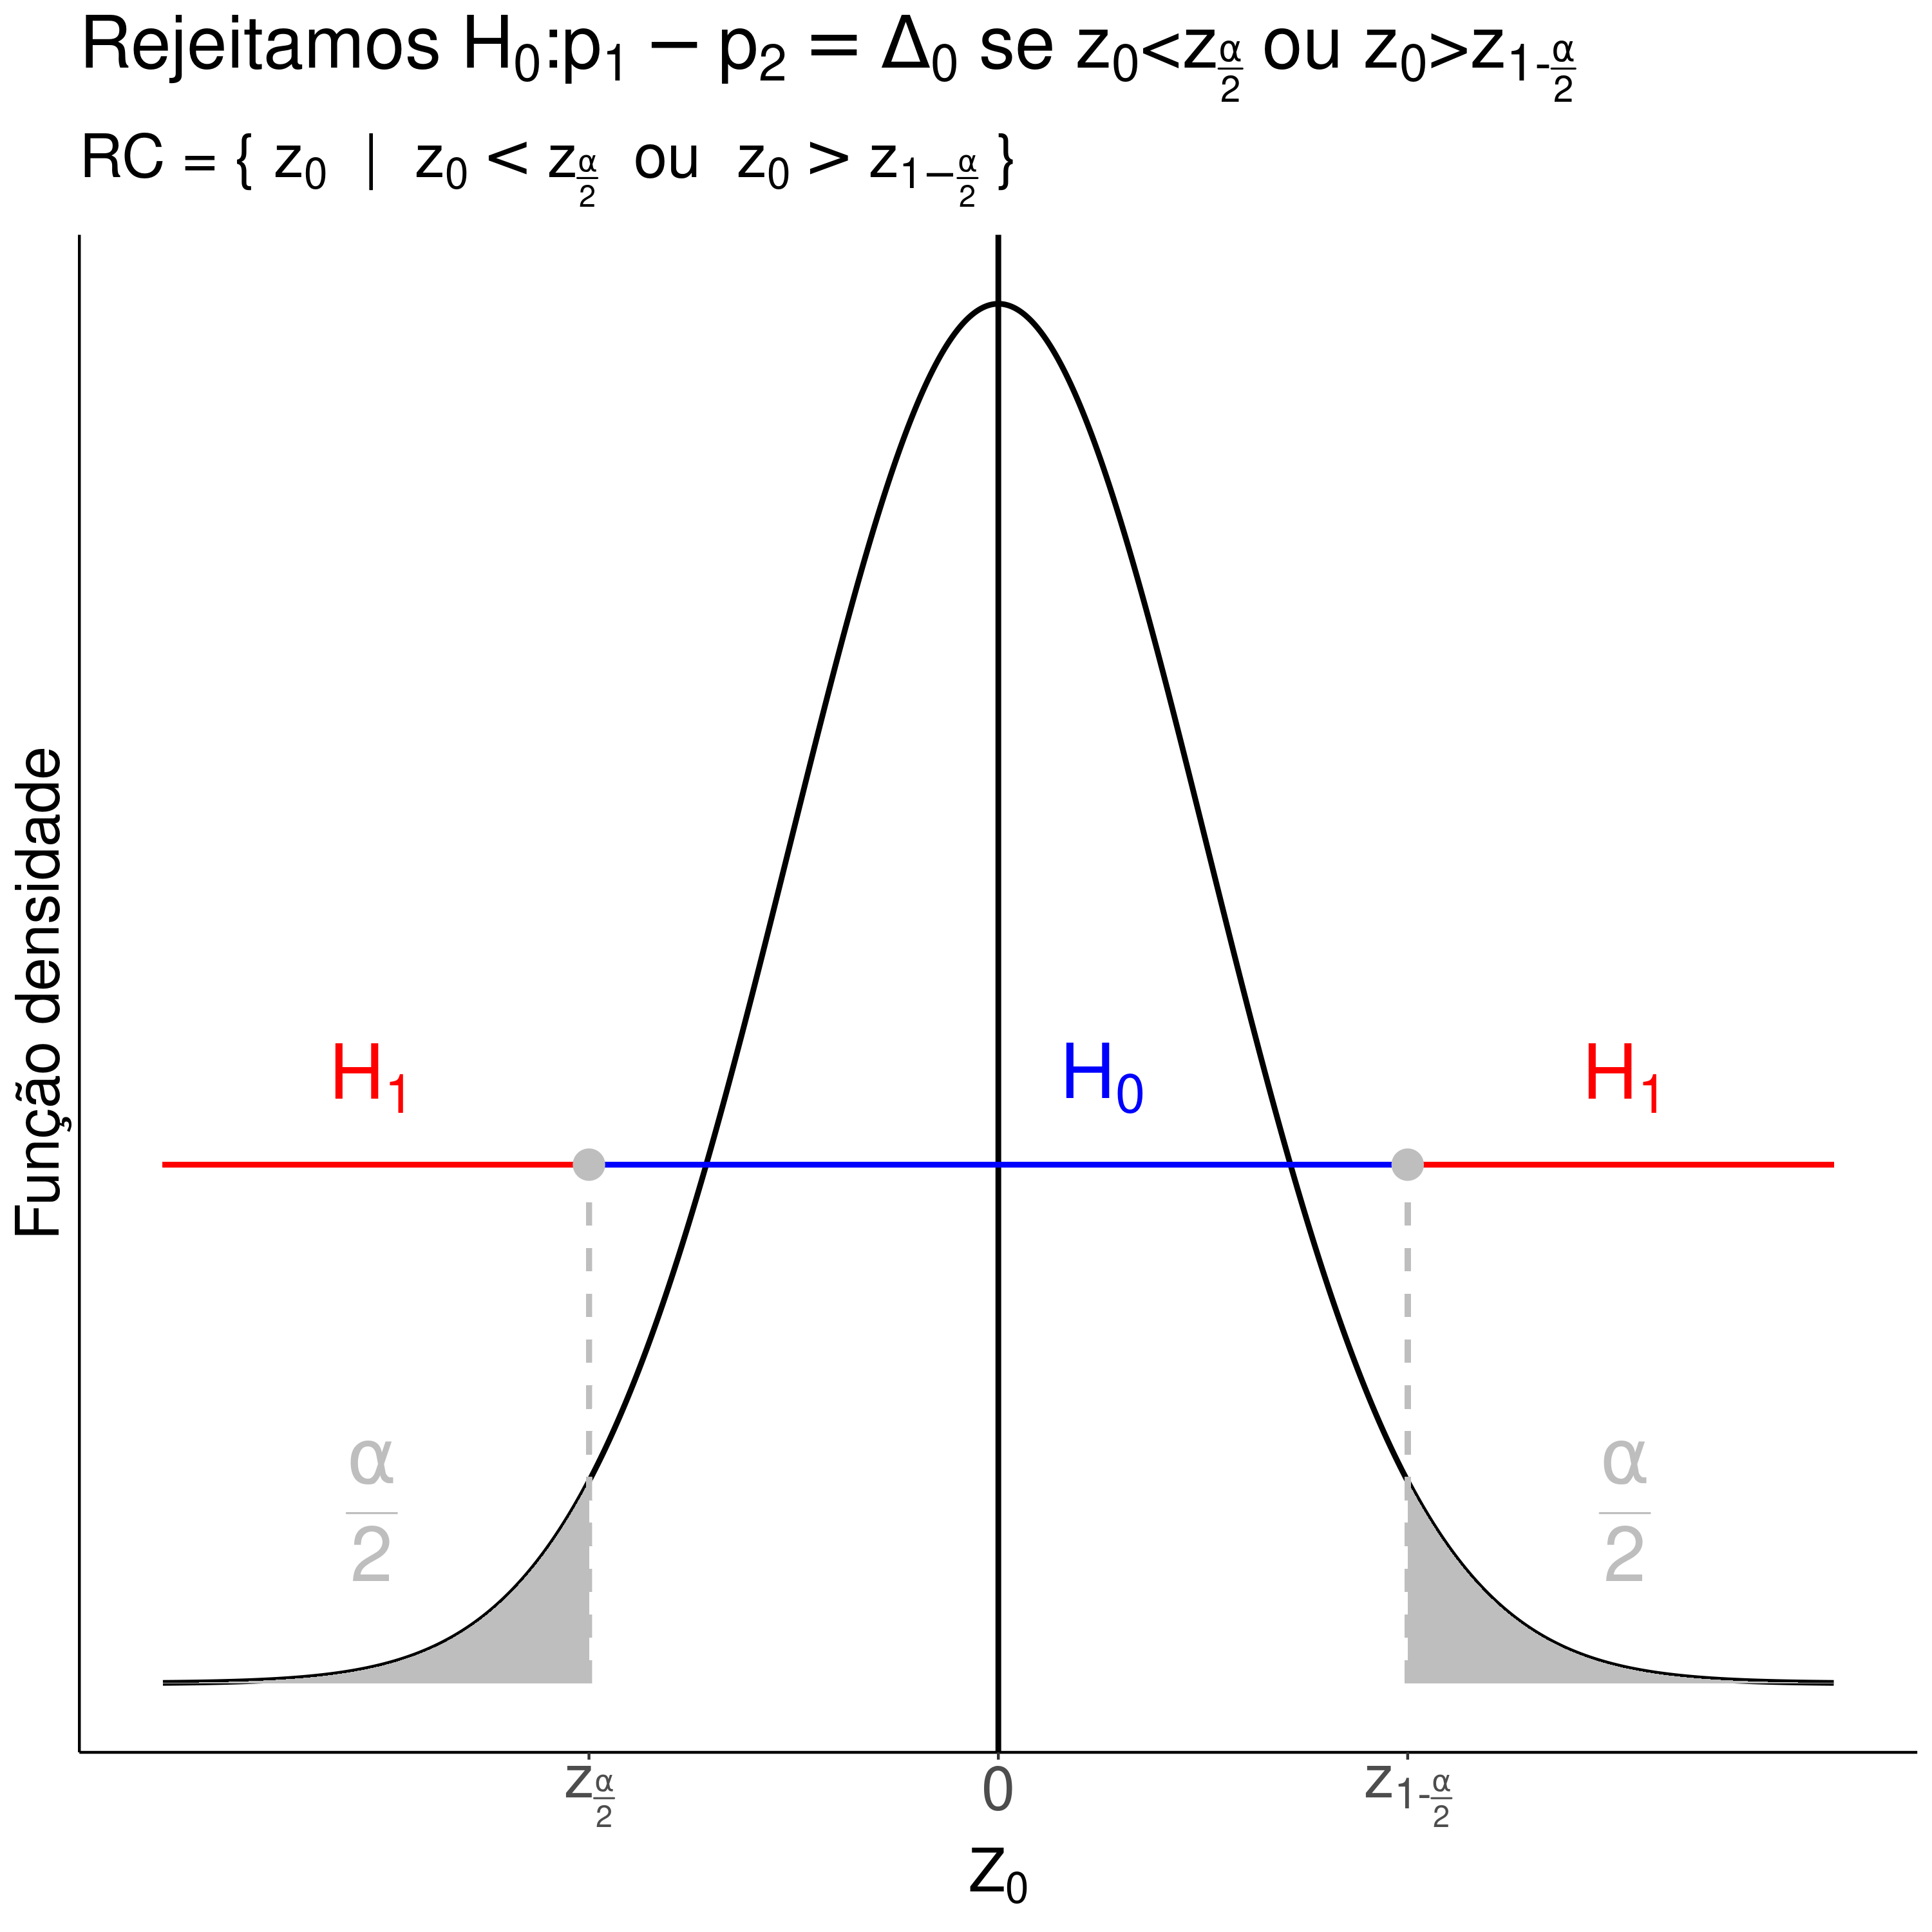
\includegraphics[width=0.32\linewidth]{figures/two-proportion-bilateral.png} \label{fig:two-proportion-bilateral}} \hfill
	\subfloat[][Teste unilateral.]{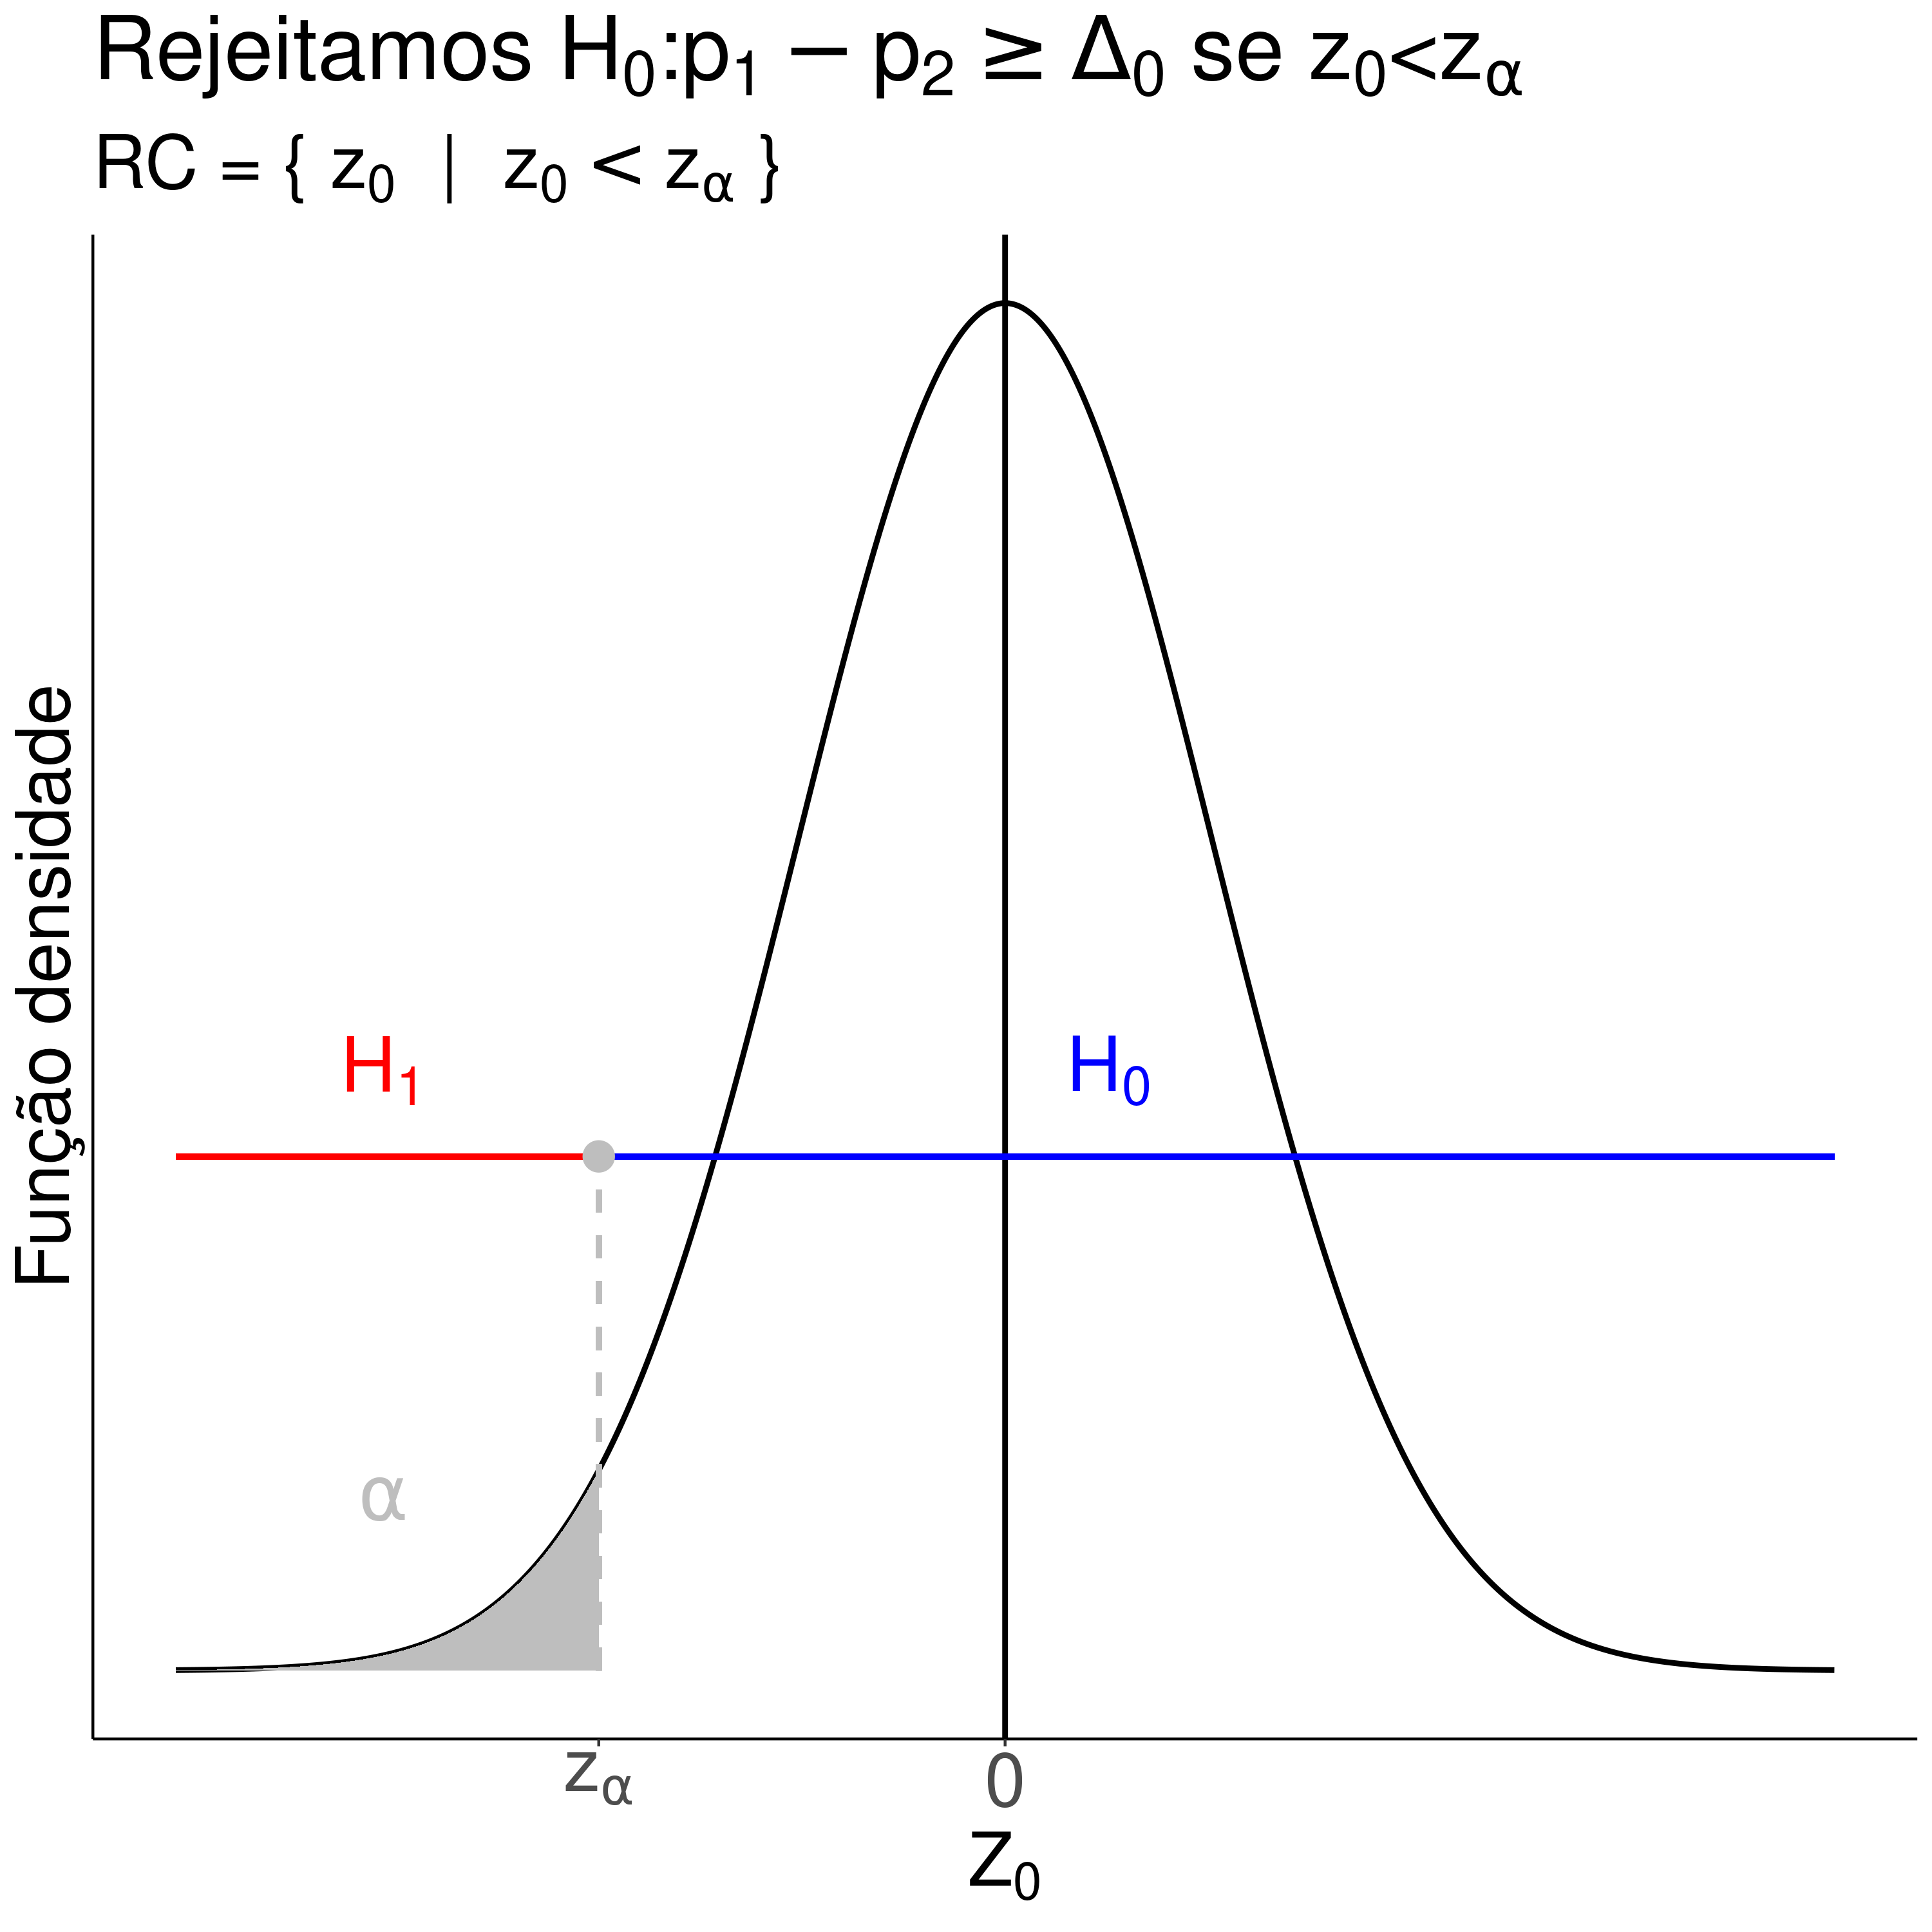
\includegraphics[width=0.32\linewidth]{figures/two-proportion-h1-lower.png} \label{fig:two-proportion-h1-lower}} \hfill
	\subfloat[][Teste unilateral.]{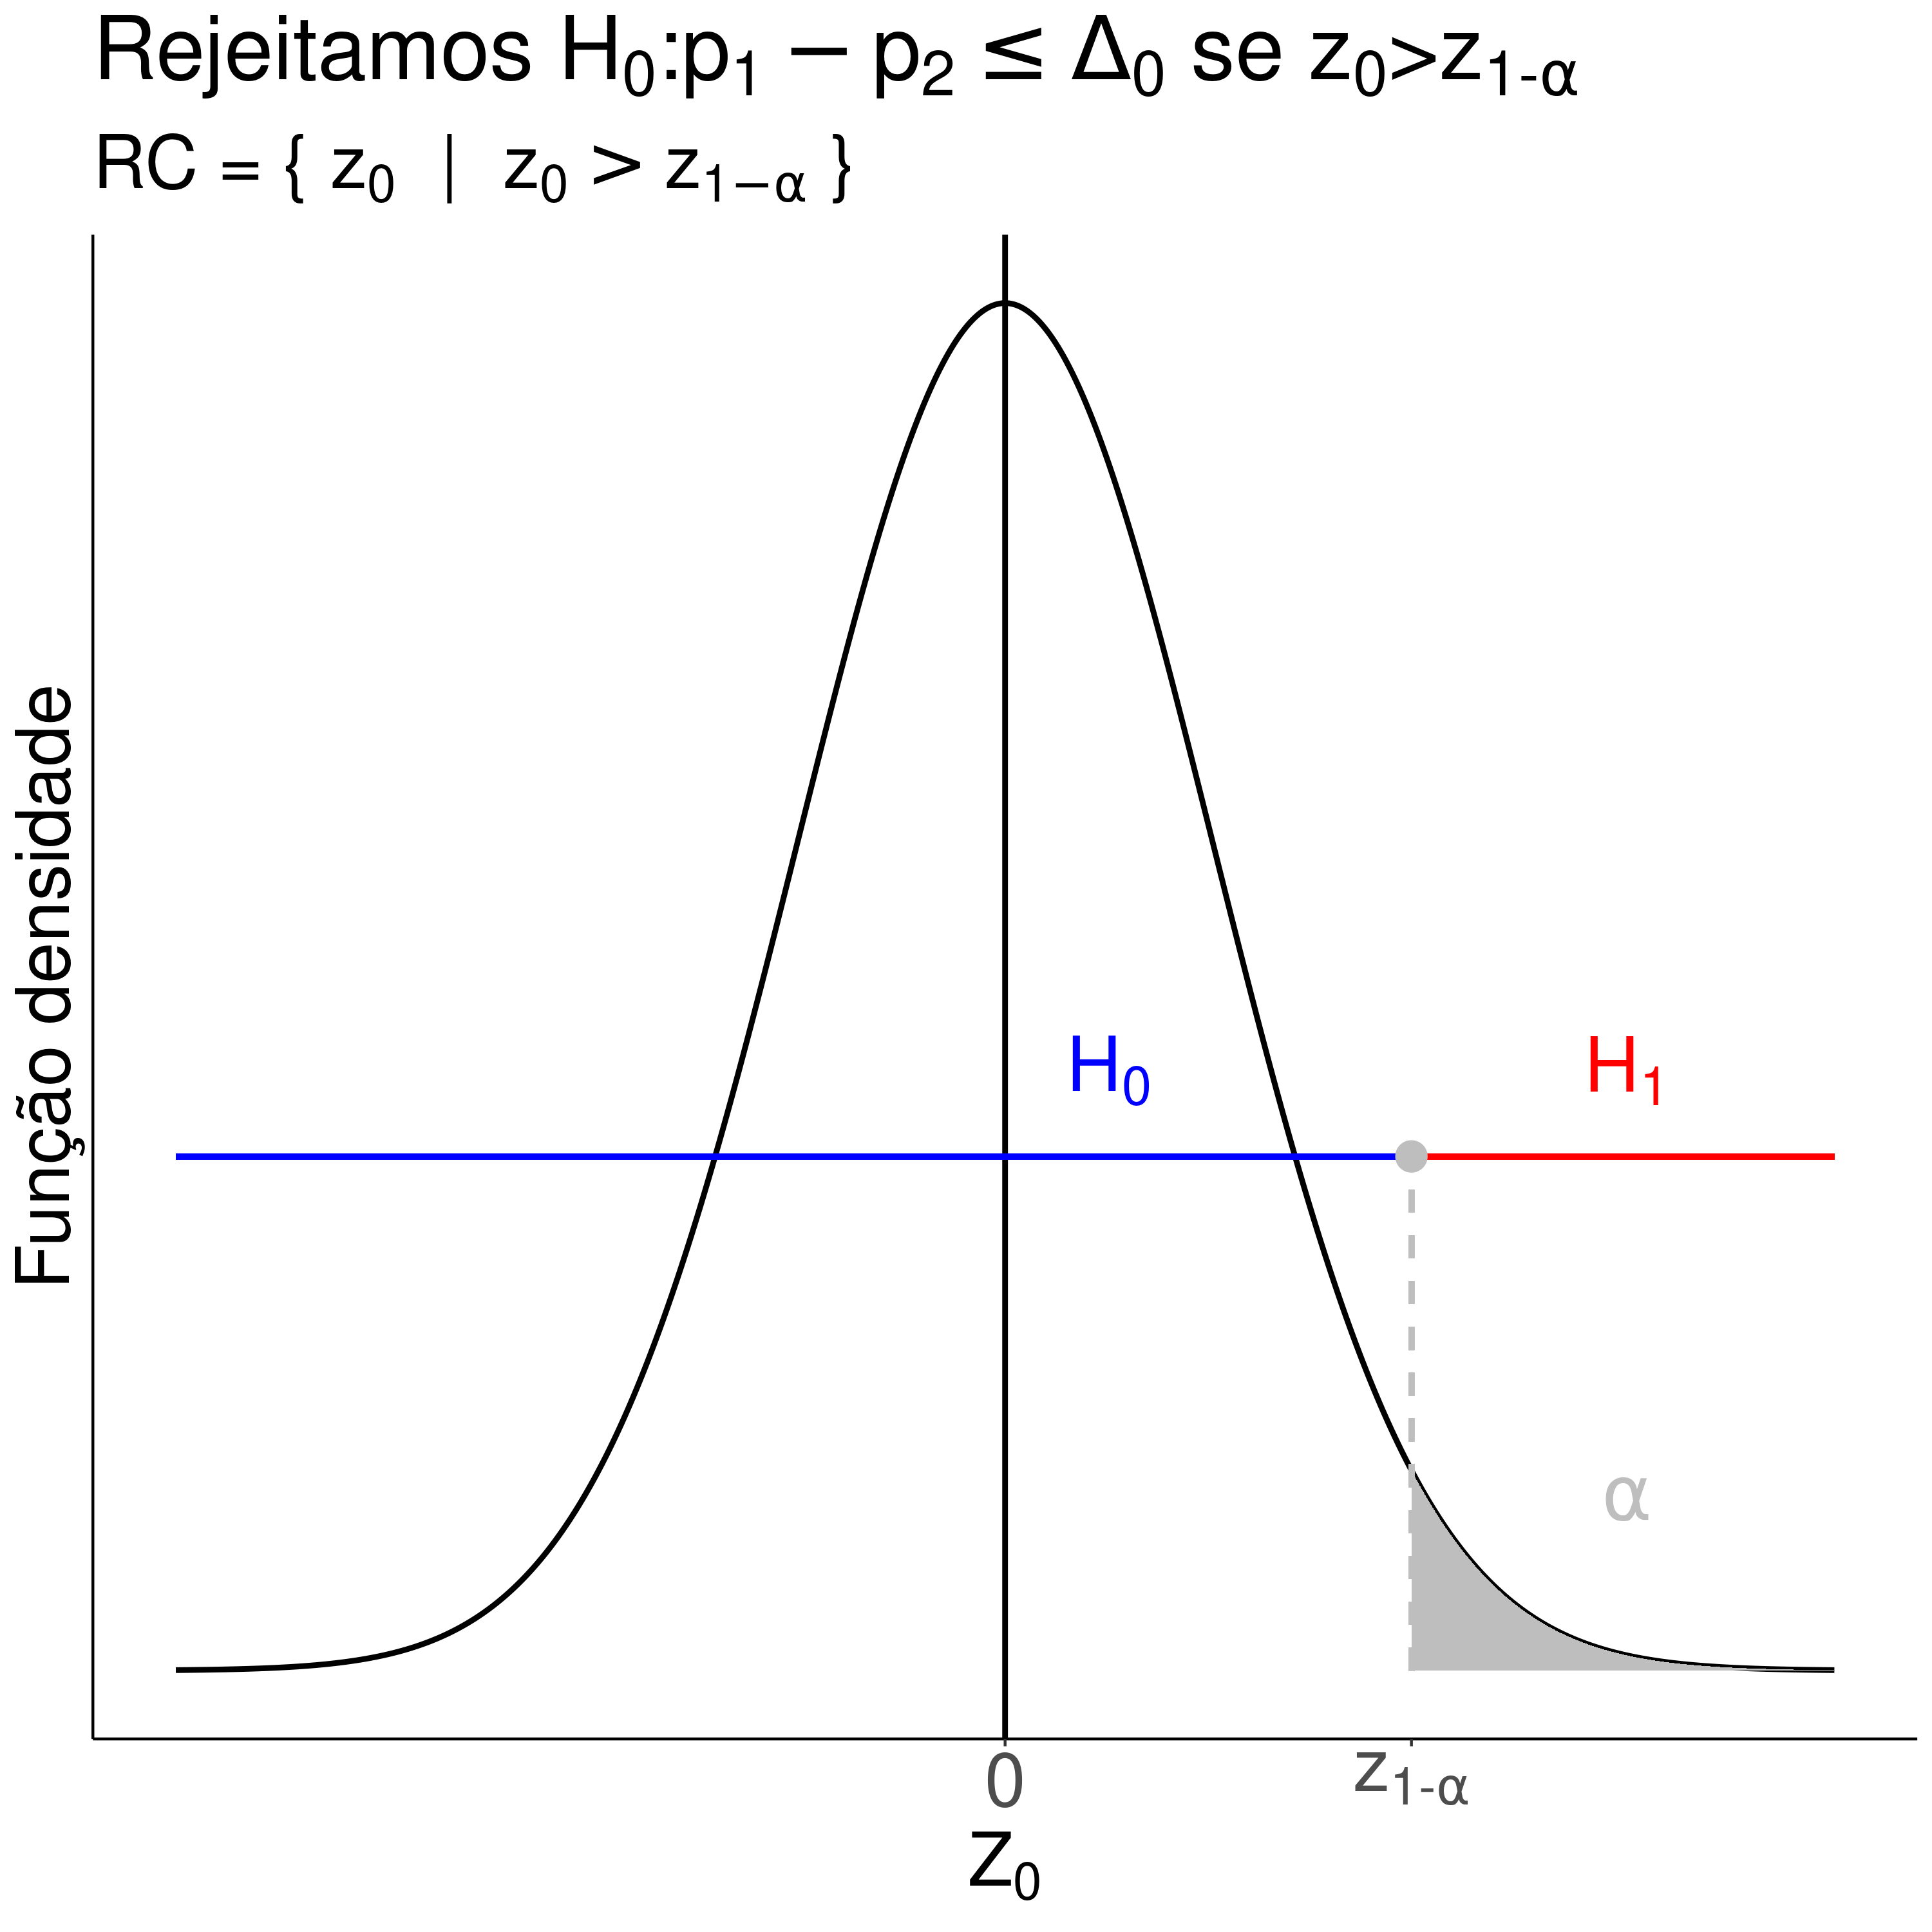
\includegraphics[width=0.32\linewidth]{figures/two-proportion-h1-upper.png} \label{fig:two-proportion-h1-upper}} 
	\caption{Região crítica para comparar médias de populações normais com variâncias desconhecidas e diferentes.}
\end{figure}

\end{frame}

\begin{frame}{Comparação de $p_1$ e $p_2$ (especialmente para $n \geq 40$).}

\begin{itemize}
	\item Na Figura~\ref{fig:two-proportion-bilateral}, testamos $H_0: p_1 - p_2 = \Delta_0$ versus $H_1: p_1 - p_2 \neq \Delta_0$. Rejeitamos $H_0$ se $z_0 = \frac{(\hat{p}_1 - \hat{p}_2 - \Delta_0)}{\sqrt{\hat{p}(1 - \hat{p})}\sqrt{\frac{1}{n_1} + \frac{1}{n_2}}} \in  RC=\{z_0 \mid z_0 < z_{\frac{\alpha}{2}} \allowbreak \mbox{ ou } z_0 > z_{1-\frac{\alpha}{2}} \}$, em que $\Phi\left( z_{\frac{\alpha}{2}} \right) = \frac{\alpha}{2}$, $\Phi\left(t_{1-\frac{\alpha}{2}} \right) = 1 - \frac{\alpha}{2}$ e $ \hat{p} = \frac{n_1 \hat{p}_1 + n_2 \hat{p}_2}{n_1 + n_2}$;
	\vfill
	
	\item Na Figura~\ref{fig:two-proportion-h1-lower}, testamos $H_0: p_1 - p_2 \leq \Delta_0 $ versus $H_1: p_1 - p_2 > \Delta_0$. Rejeitamos $H_0$ se $z_0 = \frac{(\hat{p}_1 - \hat{p}_2 - \Delta_0)}{\sqrt{\hat{p}(1 - \hat{p})}\sqrt{\frac{1}{n_1} + \frac{1}{n_2}}} \in \allowbreak RC=\{z_0 \mid z_0 > z_{1-\alpha}  \}$, em que $\Phi\left(z_{1-\alpha} \right) =1- \alpha$ e $ \hat{p} = \frac{n_1 \hat{p}_1 + n_2 \hat{p}_2}{n_1 + n_2}$;
	\vfill
	
	\item Na Figura~\ref{fig:two-proportion-h1-upper}, testamos $H_0: p_1 - p_2 \geq \Delta_0$ versus $H_1: p_1 - p_2  < \Delta_0$. Rejeitamos $H_0$ se $z_0 = \frac{(\hat{p}_1 - \hat{p}_2 - \Delta_0)}{\sqrt{\hat{p}(1 - \hat{p})}\sqrt{\frac{1}{n_1} + \frac{1}{n_2}}} \in \allowbreak RC=\{z_0 \mid z_0 < z_{\alpha}  \}$, em que $\Phi\left( z_{\alpha} \right) = \alpha$ e $ \hat{p} = \frac{n_1 \hat{p}_1 + n_2 \hat{p}_2}{n_1 + n_2}$.
\end{itemize}
Chamamos $z_\alpha$, $z_{1-\alpha}$, $z_\frac{\alpha}{2}$ e $z_{1-\frac{\alpha}{2}}$ de valores críticos.
\end{frame}

\begin{frame}{Comparação de $p_1$ e $p_2$ (especialmente para $n \geq 40$).}

\large
\begin{block}{Exemplo}
	A erva-de-são-joão (ou hipérico) tem sido usada para o tratamento de depressão por séculos. Um pesquisador decidiu estudar da erva-de-são-joão e escolheu 200 pacientes com depressão aguda: 100 pacientes foram tratados com erva-de-são-joão e 100 pacientes foram tratados com placebo. A distribuição dos pacientes foram aleatórias. Ao final do estudo, 19 pacientes com placebo se recuperam e 27 pacientes tratados com erva-de-são-joão se recuperaram. Existe evidência que a proporção de pessoas recuperadas com  erva-de-são-joão é diferente da proporção de pessoas recuperadas com placebo? Use $\alpha=5\%$. Calcule o p-valor.
\end{block}
\normalsize

\end{frame}

\begin{frame}{Comparação de $p_1$ e $p_2$ (especialmente para $n 
\geq 40$).}

\footnotesize
\begin{block}{Solução}
	Seja $p_1$ é a proporção de pessoas recuperadas usando erva-de-são-joão e $p_2$ é a proporção de pessoas recuperadas usando placebo.
	
	\textbf{Passo 1)} Queremos testar as hipóteses: $H_0: p_1 - p_2 = \Delta_0=0$ e $H_1: p_1 - p_2 \neq \Delta_0=0$;
	
	\textbf{Passo 2)} Nível de significância $\alpha=5\%$;
	
	\textbf{Passo 3)} Rejeitamos $H_0$ se $\lvert z_0 \rvert = \left\lvert \frac{(\hat{p}_1 - \hat{p}_2 - \Delta_0)}{\sqrt{\hat{p}(1 - \hat{p})}\sqrt{\frac{1}{n_1} + \frac{1}{n_2}}} \right\rvert$ for grande, em que $\hat{p} = \frac{n_1 \hat{p}_1 + n_2 \hat{p}_2}{n_1 + n_2}$. Ou seja, $RC = \left\{ z_0 \mid z_0 < z_\frac{\alpha}{2} \mbox{ ou } z_0 < z_{1-\frac{\alpha}{2}} \right\}$;
	
	\textbf{Passo 4)} Vamos encontrar os valores críticos:
	\begin{itemize}
		\item $\Phi\left( z_\frac{\alpha}{2} \right) = \Phi\left( z_{0,025} \right) = \frac{\alpha}{2} = 0,025$, então $z_{0,025} = -1,96$;
		\item $\Phi\left( z_{1-\frac{\alpha}{2}} \right) = \Phi\left( z_{0,975} \right) = 1-\frac{\alpha}{2} = 0,975$, então $z_{0,975} = 1,96$;
	\end{itemize}

	\textbf{Passo 5)} Como $\hat{p}_1 = \frac{27}{100} = 0,27$, $\hat{p_2} = \frac{19}{100}=0,19$, $n_1=n_2=100$, $\Delta_0=0$, $\hat{p} = \frac{n_1 \hat{p}_1 + n_2 \hat{p}_2}{n_1 + n_2} = \frac{100\cdot 0,27 + 100\cdot 0,19}{100 + 100} = 0,23$ e $z_0 = \frac{(\hat{p}_1 - \hat{p}_2 - \Delta_0)}{\sqrt{\hat{p}(1 - \hat{p})}\sqrt{\frac{1}{n_1} + \frac{1}{n_2}}} = \frac{(0,27 - 0,19 - 0)}{\sqrt{0,23(1 - 0,23)}\sqrt{\frac{1}{100} + \frac{1}{100}}} = 3,19 \in RC$, então rejeitamos $H_0$. 
	
	Ou seja, ao nível de significância $\alpha=5\%$, a proporção de pacientes recuperados com erva-de-são-joão e placebo são diferentes.
\end{block}
\normalsize
\end{frame}

\begin{frame}{Comparação de $p_1$ e $p_2$ (especialmente para $n 
	\geq 40$).}

\begin{block}{Solução (valor-p)}
	O valor-p pode calcular através de
	\begin{align*}
		p = P\left( \lvert Z_0 \rvert > \lvert z_0 \rvert \mid H_0 \right) = 2 \cdot \left[ 1 - \Phi(\lvert z_0 \rvert) \right].
	\end{align*}
	
	Como $\hat{p}_1 = \frac{27}{100} = 0,27$, $\hat{p_2} = \frac{19}{100}=0,19$, $n_1=n_2=100$, $\Delta_0=0$, $\hat{p} = \frac{n_1 \hat{p}_1 + n_2 \hat{p}_2}{n_1 + n_2} = \frac{100\cdot 0,27 + 100\cdot 0,19}{100 + 100} = 0,23$ e $z_0 = \frac{(\hat{p}_1 - \hat{p}_2 - \Delta_0)}{\sqrt{\hat{p}(1 - \hat{p})}\sqrt{\frac{1}{n_1} + \frac{1}{n_2}}} = \frac{(0,27 - 0,19 - 0)}{\sqrt{0,23(1 - 0,23)}\sqrt{\frac{1}{100} + \frac{1}{100}}} = 3,19$, o valor-p é dado por
	\begin{align*}
		p &= 2 \left[ 1 - \Phi \left( \lvert z_0 \rvert \right)\right]\\
		&= 2 \left[ 1 - \Phi \left( 3,19 \right)  \right]\\
		&= 2 \left[1 - 0,9993 \right]\\
		&= 0,0014.
	\end{align*}
	
	Como $p=0,0014 < \alpha = 0,05$, rejeitamos $H_0$, e a proporção de pacientes recuperados com placebo e erva-de-são-joão são diferentes.
\end{block}

\end{frame}

\begin{frame}{Comparação de $p_1$ e $p_2$ (especialmente para $n 
	\geq 40$).}

\large
\begin{block}{Exemplo}
	Um experimento tem o objetivo de avaliar a eficácia de uma cirurgia em homens diagnosticados com câncer de próstata. 347 homens diagnosticados com câncer de próstata tiveram esta cirurgia e 18 destes morreram, e 298 homens diagnosticados com câncer de próstata não tiveram esta cirurgia e 31 morreram. Existe evidência de que esta cirurgia diminui a taxa de mortalidade em homens diagnosticados com câncer próstata? Use $\alpha=5\%$. Calcule o valor-p.
\end{block}
\normalsize

\end{frame}

\begin{frame}{Comparação de $p_1$ e $p_2$ (especialmente para $n 
	\geq 40$).}

	\begin{block}{Solução}
		Seja $p_1$ é a proporção de homens diagnosticados com câncer que fizeram a cirurgia e $p_2$ é a proporção de homens diagnosticados com câncer que não fizeram a cirurgia.
		
		\textbf{Passo 1)} Queremos testar as hipóteses: $H_0: p_1 - p_2 \geq \Delta_0=0$ e $H_1: p_1 - p_2 < \Delta_0=0$;
		
		\textbf{Passo 2)} Nível de significância $\alpha=5\%$;
		
		\textbf{Passo 3)} Rejeito $H_0$ se $z_0 = \frac{\hat{p}_1 - \hat{p}_2 -\Delta_0}{\sqrt{\hat{p}(1-\hat{p}) \left( \frac{1}{n_1} + \frac{1}{n_2} \right)}}$ for pequeno. Ou seja, $RC = \left\{ z_0 \mid z_0 < z_\alpha \right\}$;
		
		\textbf{Passo 4)} Vamos calcular o valor críticos:
		\begin{itemize}
			\item $\Phi\left(z_\alpha\right) = \Phi\left(z_{0,05}\right) = \alpha = 0,05$, então $z_{0,05} = -1,65$;
		\end{itemize}
	
		\textbf{Passo 5)} Como $n_1=347$, $n_2 = 298$, $\hat{p}_1 = \frac{18}{347} = 0,05$, $\hat{p}_2 = \frac{31}{298} = 0,10$, $\Delta_0=0$, $\hat{p} = \frac{n_1 \hat{p}_1 + n_2 \hat{p}_2}{n_1 + n_2}=0,08$ e $z_0 = \frac{0,05 - 0,10 -0}{\sqrt{0,08(1-0,08) \left( \frac{1}{347} + \frac{1}{298} \right)}} = -2,33 \in RC$, então rejeitamos $H_0$. 
		
		Ou seja, ao nível de significância $\alpha=5\%$, a cirurgia diminui a taxa de mortalidade de homens com câncer de próstata.
	\end{block}

\end{frame}

\begin{frame}{Comparação de $p_1$ e $p_2$ (especialmente para $n 
	\geq 40$).}

\begin{block}{Solução (valor-p)}
	O valor-p é calculado por
	$$p = P(Z_0 < z_0 \mid H_0) = \Phi\left( z_0 \right).$$
	
	Como $n_1=347$, $n_2 = 298$, $\hat{p}_1 = \frac{18}{347} = 0,05$, $\hat{p}_2 = \frac{31}{298} = 0,10$, $\Delta_0=0$, $\hat{p} = \frac{n_1 \hat{p}_1 + n_2 \hat{p}_2}{n_1 + n_2}=0,08$ e $z_0 = \frac{0,05 - 0,10 -0}{\sqrt{0,08(1-0,08) \left( \frac{1}{347} + \frac{1}{298} \right)}} = -2,33$, então o valor-p é dado por
	\begin{align*}
		p &= \Phi\left( -2,33 \right) = 0,0099.
	\end{align*}
	
	Como $p=0,009 < \alpha = 0,05$, então rejeitamos $H_0$. Ou seja, ao nível de significância $\alpha=5\%$, a cirurgia diminui a taxa de mortalidade entre homens com câncer de próstata.
\end{block}

\end{frame}

\begin{frame}{Comparação de $p_1$ e $p_2$ (especialmente para $n 
	\geq 40$).}

\begin{block}{Exemplo}
	Um pesquisador deseja comparar duas proporções populacionais,ou seja, este pesquisador deseja decidir entre as hipóteses: $H_0: p_1 - p_2 \leq \Delta_0 =0$ e $H_1: p_1 - p_2 > \Delta_0 =0$. Algumas informações deste experimento está na Tabela~\ref{tab:h1-less-2-proportion}. Complete a Tabela~\ref{tab:h1-less-2-proportion}. Ao nível de significância $\alpha=5\%$, qual a decisão do pesquisador? Calcule o valor-p.
	\begin{table}[htbp]
		\centering
		\begin{tabular}{c|c|c|c}
			\toprule[0.05cm]
			$n_1$ & $n_2$ & $n_1 \hat{p}_1$ & $n_2 \hat{p}_2$\\ \midrule
			250 & 300 & 147 & 52 \\ \midrule[0.05cm]
			$z_0$ & $\alpha$ & Decisão & valor-p \\ \midrule
			& $5\%$ & & \\
			\bottomrule[0.05cm]
		\end{tabular}
		\caption{Algumas informações sobre experimentos.}
		\label{tab:h1-less-2-proportion}
	\end{table}
\end{block}

\end{frame}

\begin{frame}{Comparação de $p_1$ e $p_2$ (especialmente para $n 
	\geq 40$).}

\Large
\begin{block}{Solução}
	\textbf{Passo 1)} Queremos testar as seguintes hipóteses: $H_0: p_1 - p_2 \leq \Delta_0=0$ e $H_1: p_1 - p_2 > \Delta_0=0$;
	
	\textbf{Passo 2)} Nível de significância $\alpha=5\%$;
	
	\textbf{Passo 3)} Rejeitamos $H_0$ se $z_0 = \frac{\hat{p}_1 - \hat{p}_2 -\Delta_0}{\sqrt{\hat{p}(1-\hat{p}) \left( \frac{1}{n_1} + \frac{1}{n_2} \right)}}$ for grande. Ou seja, $RC = \left\{ z_0 \mid z_0 > z_{1-\alpha} \right\}$;
	
	\textbf{Passo 4)} Vamos encontrar o valor crítico:
	\begin{itemize}
		\item $\Phi\left( z_{1-\alpha} \right) = \Phi\left( z_{0,95} \right) = 1-\alpha = 0,95$, então $z_{0,95} = 1,65$;
	\end{itemize}

	\textbf{Passo 5)} Como $n_1=250$, $n_2=300$, $\hat{p}_1 = \frac{147}{250} = 0,59$, $\hat{p}_2 = \frac{52}{300} = 0,17$, $p = 0,36$ e $z_0 = \frac{0,59 - 0,17}{\sqrt{0,36(1 - 0,36) \left( \nicefrac{1}{250} + \nicefrac{1}{300} \right)}} = 10,22 \in RC$, então rejeitamos  $H_0$.
\end{block}
\normalsize
\end{frame}

\begin{frame}{Comparação de $p_1$ e $p_2$ (especialmente para $n 
	\geq 40$).}

\begin{block}{Solução (valor-p)}
	O valor-p é calculado através de 
	$$p = P \left( Z_0 > z_0 \mid H_0 \right) = 1 - \Phi \left( z_0 \right).$$
	
	Como $n_1=250$, $n_2=300$, $\hat{p}_1 = \frac{147}{250} = 0,59$, $\hat{p}_2 = \frac{52}{300} = 0,17$, $p = 0,36$ e $z_0 = \frac{0,59 - 0,17}{\sqrt{0,36(1 - 0,36) \left( \nicefrac{1}{250} + \nicefrac{1}{300} \right)}} = 10,22$, então o valor-p é dado por
	\begin{align*}
		p &= 1 - \Phi\left(z_0\right)\\
		&= 1 - \Phi\left(10,22\right)\\
		& = 1 -1\\
		&= 0.
	\end{align*}
	
	Como $p = 0 < \alpha = 0,05$, rejeitamos $H_0$.
\end{block}

\end{frame}


\subsection{Poder e tamanho da amostra.}

\begin{frame}{Poder do teste: $H_0:p_1 - p_2 = \Delta_0$ e $H_1: p_1 - p_2 \neq \Delta_0$.}

\tiny

Imagine que
\begin{itemize}
	\item Hipóteses: $H_0: p_1 - p_2 = \Delta_0$ e $H_1: p_1 -  p_2 \neq \Delta_0$;
	\item $H_1$ é verdade, então $\Delta = p_1-p_2 \neq \Delta_0$;
	\item $Z_0 = \frac{\hat{p}_1 - \hat{p}_2 - \Delta_0}{\sqrt{ 
	\frac{p_1(1-p_1)}{n_1} + \frac{p_2(1-p_2)}{n_2} }} \sim N\left( \frac{p_1 - p_2 - \Delta_0}{\sqrt{\frac{p_1(1-p_1)}{n_1} + \frac{p_2(1-p_2)}{n_2}}};1 \right)$;
	\item Ao nível de significância $\alpha$, temos $RC = \{ z_0 \mid z_0 < z_{\frac{\alpha}{2}} \mbox{ ou } z_{1-\frac{\alpha}{2}} < z_0  \}$.
\end{itemize}
\vfill	

Poder do teste é dado
\begin{align*}
\textcolor{important}{1-\beta} &=1 - \left[P\left( z_{\frac{\alpha}{2}} \leq Z_0 \leq z_{1-\frac{\alpha}{2}} \mid H_1 \right)\right] = 1 - \left[P\left( z_{\frac{\alpha}{2}} \leq Z_0 \leq z_{1-\frac{\alpha}{2}} \mid \Delta \neq \Delta_0 \right)\right]\\
&\approx \textcolor{important}{1 - \Phi\left( z_{1-\frac{\alpha}{2}} - \frac{p_1-p_2 - \Delta_0}{\sqrt{\frac{p_1(1-p_1)}{n_1} + \frac{p_2(1-p_2)}{n_2}}} \right)\ref{tab:h1-less-2-proportion-power} + \Phi\left( z_{\frac{\alpha}{2}} - \frac{p_1-p_2 - \Delta_0}{\sqrt{\frac{p_1(1-p_1)}{n_1} + \frac{p_2(1-p_2)}{n_2}}} \right).}
\end{align*}
A \textcolor{important}{Função Poder}, dado o tamanho da amostra $n$, é uma função das médias populacionais na hipótese alternativa  $\pi: \mathbb{R} - \{\Delta_0\} \longrightarrow [0,1]$ dada por
\begin{align*}
\pi(\Delta) = 1 - \Phi\left( z_{1-\frac{\alpha}{2}} - \frac{p_1-p_2 - \Delta_0}{\sqrt{\frac{p_1(1-p_1)}{n_1} + \frac{p_2(1-p_2)}{n_2}}} \right) + \Phi\left( z_{\frac{\alpha}{2}} - \frac{p_1-p_2 - \Delta_0}{\sqrt{\frac{p_1(1-p_1)}{n_1} + \frac{p_2(1-p_2)}{n_2}}} \right), \Delta = p_1 - p_2, \Delta \in \mathbb{R} - \{\Delta_0 \}.
\end{align*}
Alguns livros chamam a Função Poder de \textcolor{important}{Curva de Característica Operacional.}

\normalsize

\end{frame}


\begin{frame}{Tamanho da amostra: $H_0:p_1 - p_2 = \Delta_0$ e $H_1: p_1 - p_2 \neq \Delta_0$.}

\scriptsize
Imagine que
\begin{itemize}
	\item Hipóteses: $H_0: p_1 - p_2 = \Delta_0$ e $H_1: p_1 -  p_2 \neq \Delta_0$;
	\item $H_1$ é verdade, então $\Delta = p_1-p_2 \neq \Delta_0$;
	\item $Z_0 = \frac{\hat{p}_1 - \hat{p}_2 - \Delta_0}{\sqrt{ 
			\frac{p_1(1-p_1)}{n_1} + \frac{p_2(1-p_2)}{n_2} }} \sim N\left( \frac{p_1 - p_2 - \Delta_0}{\sqrt{\frac{p_1(1-p_1)}{n_1} + \frac{p_2(1-p_2)}{n_2}}};1 \right)$;
	\item Ao nível de significância $\alpha$, temos $RC = \{ z_0 \mid z_0 < z_{\frac{\alpha}{2}} \mbox{ ou } z_{1-\frac{\alpha}{2}} < z_0  \}$.
\end{itemize}
\vfill

Considere $1-\beta$, $\alpha$, $n_1=n_2=n$, $p_1$, $p_2$ e $\Delta_0$, então o tamanho \sout{mínimo} da amostra é solução da seguinte equação
\begin{align*}
1-\beta &= 1 - \Phi\left( z_{1-\frac{\alpha}{2}} - \frac{p_1-p_2 - \Delta_0}{\sqrt{\frac{p_1(1-p_1)}{n} + \frac{p_2(1-p_2)}{n}}} \right) + \underbrace{\Phi\left( z_{\frac{\alpha}{2}} - \frac{p_1-p_2 - \Delta_0}{\sqrt{\frac{p_1(1-p_1)}{n} + \frac{p_2(1-p_2)}{n}}} \right)}_{\approx 0}\\
&\approx 1 - \Phi\left( z_{1-\frac{\alpha}{2}} - \frac{p_1-p_2 - \Delta_0}{\sqrt{\frac{p_1(1-p_1)}{n} + \frac{p_2(1-p_2)}{n}}} \right)
\end{align*}
em que 
$$n = \left\lceil \frac{(z_{1-\frac{\alpha}{2}} + z_{1-\beta})^2 \left( p_1(1 - p_1) + p_2(1 - p_2) \right)}{\left(p_1 - p_2 - \Delta_0\right)^2} \right\rceil $$
\normalsize

\end{frame}


\begin{frame}{Poder do teste: $H_0:p_1 - p_2 = \Delta_0$ e $H_1: p_1 - p_2 \neq \Delta_0$.}

\large
\begin{block}{Exemplo}
	A erva-de-são-joão (ou hipérico) tem sido usada para o tratamento de depressão por séculos. Um pesquisador deseja estudar da erva-de-são-joão e escolheu 200 pacientes com depressão aguda: 100 pacientes foram tratados com erva-de-são-joão e 100 pacientes foram tratados com placebo. 
%	A distribuição dos pacientes foram aleatórias. Ao final do estudo, 19 pacientes com placebo se recuperam e 27 pacientes tratados com erva-de-são-joão se recuperaram. 
Imagine que a proporção de pacientes com depressão que se recuperam ao usar erva-de-são-joão  é $p_1 = 0,3$ e a proporção de pacientes com depressão que se recuperam usando placebo é $p_2 = 0,15$. 
	Qual o poder do teste? Use $\alpha=5\%$.
\end{block}
\normalsize
\end{frame}

\begin{frame}{Poder do teste: $H_0:p_1 - p_2 = \Delta_0$ e $H_1: p_1 - p_2 \neq \Delta_0$.}

\small

\begin{block}{Solução}
	\textbf{Passo 1)} Queremos testar as seguintes hipóteses: $H_0: p_1 - p_2 = \Delta_0=0$ e $H_1: p_1 - p_2 \neq \Delta_0=0$;
	
	\textbf{Passo 2)} Nível de significância $\alpha=5\%$;
	
	\textbf{Passo 3)} Rejeitamos $H_0$ se $Z_0 = \frac{\hat{p}_1 - \hat{p}_2 - \Delta_0}{\sqrt{\frac{p_1(1-p_1)}{n_1} + \frac{p_2(1-p_2)}{n_2}}}$. Ou seja, $RC = \left\{ z_0 \mid z_0 < z_\frac{\alpha}{2} \mbox{ ou } z_0 < z_{1-\frac{\alpha}{2}} \right\}$;
	
	\textbf{Passo 4)} Queremos encontrar os valores críticos:
	\begin{itemize}
		\item $\Phi\left( z_\frac{\alpha}{2}\right) = \Phi\left( z_{0,025}\right) = \frac{\alpha}{2} = 0,025$, então $z_{0,025} = -1,96$;
		\item $\Phi\left( z_{1-\frac{\alpha}{2}}\right) = \Phi\left( z_{0,975}\right) =1- \frac{\alpha}{2} = 0,975$, então $z_{0,975} = 1,96$.
	\end{itemize}
\end{block}

Como $p_1 = 0,3$, $p_2=0,15$, $n_1=n_2=100$, $\alpha = 0,05$ e $\Delta_0=0$, temos que
\tiny
\begin{align*}
	1-\beta &= 1 - \Phi\left( z_{1-\frac{\alpha}{2}} - \frac{p_1-p_2 - \Delta_0}{\sqrt{\frac{p_1(1-p_1)}{n_1} + \frac{p_2(1-p_2)}{n_2}}} \right) + \Phi\left( z_{\frac{\alpha}{2}} - \frac{p_1-p_2 - \Delta_0}{\sqrt{\frac{p_1(1-p_1)}{n_1} + \frac{p_2(1-p_2)}{n_2}}} \right)\\
	&= 1 - \Phi\left( z_{0,975} - \frac{0,3-0,15 - 0}{\sqrt{\frac{0,3(1-0,3)}{100} + \frac{0,15(1-0,15)}{100}}} \right) + \Phi\left( z_{0,025} - \frac{0,3-0,15 - 0}{\sqrt{\frac{0,3(1-0,3)}{100} + \frac{0,15(1-0,15)}{100}}} \right)\\
	&= 0,7330.
\end{align*}
\normalsize
\end{frame}


\begin{frame}{Tamanho da amostra: $H_0:p_1 - p_2 = \Delta_0$ e $H_1: p_1 - p_2 \neq \Delta_0$.}

\large
\begin{block}{Exemplo}
	A erva-de-são-joão (ou hipérico) tem sido usada para o tratamento de depressão por séculos. Um pesquisador deseja estudar a erva-de-são-joão e escolherá $2\cdot n$ pacientes com depressão aguda: $n$ pacientes serão tratados com erva-de-são-joão e $n$ pacientes serão tratados com placebo. 
	%	A distribuição dos pacientes foram aleatórias. Ao final do estudo, 19 pacientes com placebo se recuperam e 27 pacientes tratados com erva-de-são-joão se recuperaram. 
	Imagine que a proporção de pacientes com depressão que se recuperam ao usar erva-de-são-joão é $p_1 = 0,3$ e a proporção de pacientes com depressão que se recuperam usando placebo é $p_2 = 0,15$. 
	Qual o valor de $n$ para termos o poder de teste com $1-\beta = 99\%$? Use $\alpha=5\%$.
\end{block}
\normalsize

\end{frame}

\begin{frame}{Tamanho da amostra: $H_0:p_1 - p_2 = \Delta_0$ e $H_1: p_1 - p_2 \neq \Delta_0$.}

\normalsize
\begin{block}{Solução}
	\textbf{Passo 1)} Queremos testar as seguintes hipóteses: $H_0: p_1 - p_2 = \Delta_0=0$ e $H_1: p_1 - p_2 \neq \Delta_0=0$;
	
	\textbf{Passo 2)} Nível de significância $\alpha=5\%$;
	
	Como $p_1 = 0,3$, $p_2=0,15$, $n_1=n_2=n$, $\alpha = 0,05$ e $\Delta_0=0$, $1-\beta=99\%$, então
	\begin{itemize}
		\item $\Phi\left( z_{1-\frac{\alpha}{2}}\right) = \Phi\left( z_{0,975}\right) =1- \frac{\alpha}{2} = 0,975$, então $z_{0,975} = 1,96$;
		\item $\Phi\left( z_{1-\beta}\right) = \Phi\left( z_{0,99}\right) =1- \beta = 0,99$, então $z_{0,99} = 2,33$.
	\end{itemize}
	
	Então, o tamanho \sout{mínimo} de amostra é dado por
	\begin{align*}
		n &= \frac{(z_{1-\frac{\alpha}{2}} + z_{1-\beta})^2 \left( p_1(1 - p_1) + p_2(1 - p_2) \right)}{\left(p_1 - p_2 - \Delta_0\right)^2}\\
		&= \frac{(1,96 + 2,33)^2 \left( 0,3(1 - 0,3) + 0,15(1 - 0,15) \right)}{\left(0,3 - 0,15 - 0\right)^2}\\
		&= \left \lceil 276,0615 \right\rceil = 277.
	\end{align*}
\end{block}
\normalsize

\end{frame}

\begin{frame}{Poder do teste: $H_0:p_1 - p_2 \leq \Delta_0$ e $H_1: p_1 - p_2 > \Delta_0$.}

\footnotesize

Imagine que
\begin{itemize}
	\item Hipóteses: $H_0: p_1 - p_2 \leq \Delta_0$ e $H_1: p_1 -  p_2 > \Delta_0$;
	\item $H_1$ é verdade, então $\Delta = p_1-p_2 \neq \Delta_0$;
	\item $Z_0 = \frac{\hat{p}_1 - \hat{p}_2 - \Delta_0}{\sqrt{ 
			\frac{p_1(1-p_1)}{n_1} + \frac{p_2(1-p_2)}{n_2} }} \sim N\left( \frac{p_1 - p_2 - \Delta_0}{\sqrt{\frac{p_1(1-p_1)}{n_1} + \frac{p_2(1-p_2)}{n_2}}};1 \right)$;
	\item Ao nível de significância $\alpha$, temos $RC = \{ z_0 \mid z_0 > z_{1-\alpha}  \}$.
\end{itemize}
\vfill	

Poder do teste é dado
\begin{align*}
\textcolor{important}{1-\beta} &=1 - \left[P\left(  Z_0 \leq z_{1-\alpha} \mid H_1 \right)\right] = 1 - \left[P\left( Z_0 \leq z_{1-\alpha} \mid \Delta \neq \Delta_0 \right)\right]\\
&= \textcolor{important}{1 - \Phi\left( z_{1-\alpha} - \frac{p_1-p_2 - \Delta_0}{\sqrt{\frac{p_1(1-p_1)}{n_1} + \frac{p_2(1-p_2)}{n_2}}} \right).}
\end{align*}
A \textcolor{important}{Função Poder}, dado o tamanho da amostra $n$, é uma função das médias populacionais na hipótese alternativa  $\pi: (\Delta_0, \infty) \longrightarrow [0,1]$ dada por
\begin{align*}
\pi(\Delta) = 1 - \Phi\left( z_{1-\alpha} - \frac{p_1-p_2 - \Delta_0}{\sqrt{\frac{p_1(1-p_1)}{n_1} + \frac{p_2(1-p_2)}{n_2}}} \right), \Delta = p_1 - p_2, \Delta \in (\Delta_0, \infty).
\end{align*}
Alguns livros chamam a Função Poder de \textcolor{important}{Curva de Característica Operacional.}

\normalsize

\end{frame}


\begin{frame}{Tamanho da amostra: $H_0:p_1 - p_2 \leq \Delta_0$ e $H_1: p_1 - p_2 > \Delta_0$.}

Imagine que
\begin{itemize}
	\item Hipóteses: $H_0: p_1 - p_2 \leq \Delta_0$ e $H_1: p_1 -  p_2 > \Delta_0$;
	\item $H_1$ é verdade, então $\Delta = p_1-p_2 \neq \Delta_0$;
	\item $Z_0 = \frac{\hat{p}_1 - \hat{p}_2 - \Delta_0}{\sqrt{ 
			\frac{p_1(1-p_1)}{n_1} + \frac{p_2(1-p_2)}{n_2} }} \sim N\left( \frac{p_1 - p_2 - \Delta_0}{\sqrt{\frac{p_1(1-p_1)}{n_1} + \frac{p_2(1-p_2)}{n_2}}};1 \right)$;
	\item Ao nível de significância $\alpha$, temos $RC = \{ z_0 \mid z_0 > z_{1-\alpha}  \}$.
\end{itemize}
\vfill

Considere $1-\beta$, $\alpha$, $n_1=n_2=n$, $p_1$, $p_2$ e $\Delta_0$, então o tamanho \sout{mínimo} da amostra é solução da seguinte equação
\begin{align*}
1-\beta = 1 - \Phi\left( z_{1-\alpha} - \frac{p_1-p_2 - \Delta_0}{\sqrt{\frac{p_1(1-p_1)}{n} + \frac{p_2(1-p_2)}{n}}} \right),
\end{align*}
e
\begin{align*}
n = \left\lceil \frac{\left( z_{1-\alpha} + z_{1-\beta} \right)^2 \left( p_1(1 - p_1) + p_2(1 - p_2) \right)}{\left(p_1 - p_2 - \Delta_0\right)^2} \right\rceil.
\end{align*}
\end{frame}

\begin{frame}{Poder do teste: $H_0:p_1 - p_2 \leq \Delta_0$ e $H_1: p_1 - p_2 > \Delta_0$.}

\begin{block}{Exemplo}
	Um pesquisador deseja comparar duas proporções populacionais,ou seja, este pesquisador deseja decidir entre as hipóteses: $H_0: p_1 - p_2 \leq \Delta_0 =0$ e $H_1: p_1 - p_2 > \Delta_0 =0$. Algumas informações deste experimento está na Tabela~\ref{tab:h1-less-2-proportion-power}. Complete a Tabela~\ref{tab:h1-less-2-proportion-power}. Qual o poder do teste? 
	\begin{table}[htbp]
		\centering
		\begin{tabular}{c|c|c|c|c|c}
			\toprule[0.05cm]
			$n_1$ & $n_2$ & $\alpha$ & $1-\beta$ & $p_1$ & $p_2$ \\ \midrule
			250 & 300 & $5\%$ &  & $0,5$  & $0,2$ \\ \bottomrule[0.05cm]
		\end{tabular}
		\caption{Algumas informações sobre experimentos.}
		\label{tab:h1-less-2-proportion-power}
	\end{table}
\end{block}

\end{frame}

\begin{frame}{Poder do teste: $H_0:p_1 - p_2 \leq \Delta_0$ e $H_1: p_1 - p_2 > \Delta_0$.}

\begin{block}{Solução}
	\textbf{Passo 1)} Queremos testar as hipóteses: $H_0: p_1 - p_2 \leq \Delta_0$ e $H_1: p_1 - p_2 > \Delta_0$.
	
	\textbf{Passo 2)} Nível de significância $\alpha=5\%$;
	
	Como $n_1=250$, $n_2 = 300$, $\alpha = 0,05$, $p_1 = 0,5$, $p_2 =0,2$ e $\Delta_0=0$. Primeiro, vamos calcular o quantil da distribuição normal
	\begin{itemize}
		\item $\Phi\left( z_{1-\alpha}  \right) = \Phi\left( z_{0,95}  \right) = 1- \alpha = 0,95$, então $z_{0,95}  = 1,65$.
	\end{itemize} 

	Então, o poder do teste é dado por
	\begin{align*}
		1 - \beta &= 1 - \Phi \left( z_{1-\alpha} - \frac{p_1 - p_2 - \Delta_0}{\sqrt{\frac{p_1(1 - p_1)}{n_1} + \frac{p_2(1 - p_2)}{n_2}}} \right) \\
		&= 1 - \Phi \left( 1,65 - \frac{0,5 - 0,2 - 0}{\sqrt{\frac{0,5(1 - 0,5)}{250} + \frac{0,2(1 - 0,2)}{300}}} \right) \\ 
		&=1 - \Phi(-6,01) = 1.
	\end{align*}
\end{block}

\end{frame}

\begin{frame}{Tamanho da amostra: $H_0:p_1 - p_2 \leq \Delta_0$ e $H_1: p_1 - p_2 > \Delta_0$.}

\begin{block}{Exemplo}
	Um pesquisador deseja comparar duas proporções populacionais,ou seja, este pesquisador deseja decidir entre as hipóteses: $H_0: p_1 - p_2 \leq \Delta_0 =0$ e $H_1: p_1 - p_2 > \Delta_0 =0$. Algumas informações deste experimento está na Tabela~\ref{tab:h1-less-2-proportion-sample-size}. Complete a Tabela~\ref{tab:h1-less-2-proportion-sample-size}. Dado o poder do teste $1-\beta=99\%$, quantas observações precisamos coletar de cada variável? Use $\alpha=5\%$. 
	\begin{table}[htbp]
		\centering
		\begin{tabular}{c|c|c|c|c}
			\toprule[0.05cm]
			$n_1=n_2=n$ & $\alpha$ & $1-\beta$ & $p_1$ & $p_2$ \\ \midrule
			 & $5\%$ & $99\%$ & $0,5$  & $0,2$ \\ \bottomrule[0.05cm]
		\end{tabular}
		\caption{Algumas informações sobre experimentos.}
		\label{tab:h1-less-2-proportion-sample-size}
	\end{table}
\end{block}

\end{frame}

\begin{frame}{Tamanho da amostra: $H_0:p_1 - p_2 \leq \Delta_0$ e $H_1: p_1 - p_2 > \Delta_0$.}

\begin{block}{Solução}
	\textbf{Passo 1)} Queremos testar as seguintes hipóteses: $H_0: p_1 - p_2 \leq \Delta_0 = 0$ e $H_1: p_1 - p_2 > \Delta_0 = 0$;
	
	\textbf{Passo 2)} Nível de significância $\alpha=5\%$;
	
	Como $n_1=n_2=n$, $\alpha=0,05$, $1-\beta = 0,99$, $p_1 = 0,5$, $p_2 = 0,2$ e $\Delta_0=0$. Primeiro encontramos os quantis da distribuição normal
	\begin{itemize}
		\item $\Phi\left( z_{1-\beta} \right) = \Phi\left( z_{0,99} \right) = 1-\beta = 0,99$, então $z_{0,99} = 2,33$;
		\item $\Phi\left( z_{1-\alpha} \right) = \Phi\left( z_{0,95} \right) = 1-\alpha = 0,95$, então $z_{0,95} = 1,65$.
	\end{itemize}

	Então, para cada população precisamos coletar:
	\begin{align*}
	n &= \left\lceil \frac{\left(z_{1-\alpha} + z_{1-\beta}  \right)^2 \left( p_1(1 - p_1) + p_2(1 - p_2) \right)}{\left( p_1 -p_2 - \Delta_0 \right)^2} \right\rceil\\
	&= \left\lceil \frac{\left(1,65 + 2,33  \right)^2 \left( 0,5(1 - 0,5) + 0,2(1 - 0,2) \right)}{\left( 0,5 -0,2 - 0 \right)^2} \right\rceil\\
	&= \lceil 72,16  \rceil = 73.
	\end{align*}
	
\end{block}

\end{frame}

\begin{frame}{Poder do teste: $H_0:p_1 - p_2 \geq \Delta_0$ e $H_1: p_1 - p_2 < \Delta_0$.}

\footnotesize

Imagine que
\begin{itemize}
	\item Hipóteses: $H_0: p_1 - p_2 \geq \Delta_0$ e $H_1: p_1 -  p_2 < \Delta_0$;
	\item $H_1$ é verdade, então $\Delta = p_1-p_2 \neq \Delta_0$;
	\item $Z_0 = \frac{\hat{p}_1 - \hat{p}_2 - \Delta_0}{\sqrt{ 
			\frac{p_1(1-p_1)}{n_1} + \frac{p_2(1-p_2)}{n_2} }} \sim N\left( \frac{p_1 - p_2 - \Delta_0}{\sqrt{\frac{p_1(1-p_1)}{n_1} + \frac{p_2(1-p_2)}{n_2}}};1 \right)$;
	\item Ao nível de significância $\alpha$, temos $RC = \{ z_0 \mid z_0 < z_{\alpha}  \}$.
\end{itemize}
\vfill	

Poder do teste é dado
\begin{align*}
\textcolor{important}{1-\beta} &=1 - \left[P\left(  Z_0 \geq z_{\alpha} \mid H_1 \right)\right] = \left[P\left( Z_0 \leq z_{\alpha} \mid \Delta \neq \Delta_0 \right)\right]= \textcolor{important}{\Phi\left( z_{\alpha} - \frac{p_1-p_2 - \Delta_0}{\sqrt{\frac{p_1(1-p_1)}{n_1} + \frac{p_2(1-p_2)}{n_2}}} \right).}
\end{align*}
A \textcolor{important}{Função Poder}, dado o tamanho da amostra $n$, é uma função das médias populacionais na hipótese alternativa  $\pi: (-2, \Delta_0) \longrightarrow [0,1]$ dada por
\begin{align*}
\pi(\delta) = \Phi\left( z_{1-\alpha} - \frac{p_1-p_2 - \Delta_0}{\sqrt{\frac{p_1(1-p_1)}{n_1} + \frac{p_2(1-p_2)}{n_2}}} \right), \Delta = p_1 - p_2, \Delta \in (-2, \Delta_0).
\end{align*}
Alguns livros chamam a Função Poder de \textcolor{important}{Curva de Característica Operacional.}

\normalsize

\end{frame}


\begin{frame}{Tamanho da amostra: $H_0:p_1 - p_2 \geq \Delta_0$ e $H_1: p_1 - p_2 < \Delta_0$.}

Imagine que
\begin{itemize}
\item Hipóteses: $H_0: p_1 - p_2 \geq \Delta_0$ e $H_1: p_1 -  p_2 < \Delta_0$;
\item $H_1$ é verdade, então $\Delta = p_1-p_2 \neq \Delta_0$;
\item $Z_0 = \frac{\hat{p}_1 - \hat{p}_2 - \Delta_0}{\sqrt{ 
		\frac{p_1(1-p_1)}{n_1} + \frac{p_2(1-p_2)}{n_2} }} \sim N\left( \frac{p_1 - p_2 - \Delta_0}{\sqrt{\frac{p_1(1-p_1)}{n_1} + \frac{p_2(1-p_2)}{n_2}}};1 \right)$;
\item Ao nível de significância $\alpha$, temos $RC = \{ z_0 \mid z_0 < z_{\alpha}  \}$.
\end{itemize}
\vfill

Considere $1-\beta$, $\alpha$, $n_1=n_2=n$, $p_1$, $p_2$ e $\Delta_0$, então o tamanho \sout{mínimo} da amostra é solução da seguinte equação
\begin{align*}
1-\beta = \Phi\left( z_{\alpha} - \frac{p_1-p_2 - \Delta_0}{\sqrt{\frac{p_1(1-p_1)}{n} + \frac{p_2(1-p_2)}{n}}} \right),
\end{align*}
e
\begin{align*}
n = \left\lceil \frac{\left( z_{1-\alpha} + z_{1-\beta} \right)^2 \left( p_1(1 - p_1) + p_2(1 - p_2) \right)}{\left(p_1 - p_2 - \Delta_0\right)^2} \right\rceil.
\end{align*}
\end{frame}

\begin{frame}{Poder do teste: $H_0:p_1 - p_2 \geq \Delta_0$ e $H_1: p_1 - p_2 < \Delta_0$.}
\begin{block}{Exemplo}
	Um experimento tem o objetivo de avaliar a eficácia de uma cirurgia em homens diagnosticados com câncer de próstata. 347 homens diagnosticados com câncer de próstata tiveram esta cirurgia  e 298 homens diagnosticados com câncer de próstata não tiveram esta cirurgia. Imagine que a taxa de mortalidade de homens com câncer de próstata que fizeram a cirurgia é $p_1=5\%$ e a taxa de mortalidade de homens com câncer de próstata que não fizeram cirurgia é $p_2=10\%$. Qual o poder do teste? Use $\alpha=5\%$.
\end{block}
\end{frame}

\begin{frame}{Poder do teste: $H_0:p_1 - p_2 \geq \Delta_0$ e $H_1: p_1 - p_2 < \Delta_0$.}

\begin{block}{Solução}
	Seja $p_1$ é a taxa de mortalidade de homens com câncer de próstata que fizeram a cirurgia e $p_2$ é a taxa de mortalidade de homens com câncer de próstata que não fizeram a cirurgia.
	
	\textbf{Passo 1)} Queremos testar as hipóteses: $H_0: p_1 - p_2 \geq \Delta_0=0$ e $H_0: p_1 - p_2 < \Delta_0=0$;
	
	\textbf{Passo 2)} Nível de significância $\alpha=5\%$;
	
	Como $n_1=347$, $n_2=298$, $p_1=0,05$ e $p_2=0,1$. Primeiro calculamos o quantil da distribuição normal:
	\begin{itemize}
		\item $\Phi\left(z_{\alpha}\right) = \Phi\left(z_{0,05}\right) = \alpha = 0,05$, então $z_{0,05} = -1,65$.
	\end{itemize}
	Então, o poder do teste é dado por
	\begin{align*}
	1-\beta &= \Phi\left( z_{\alpha} - \frac{p_1-p_2 - \Delta_0}{\sqrt{\frac{p_1(1-p_1)}{n_1} + \frac{p_2(1-p_2)}{n_2}}} \right)\\
	&= \Phi \left( -1,65 - \frac{0,05 - 0,1 - 0}{ \sqrt{\frac{0,05(1-0,05)}{347} + \frac{0,1(1-0,1)}{298}}}  \right)= \Phi \left( 0,74 \right) = 0,7704.
	\end{align*}
\end{block}

\end{frame}

\begin{frame}{Tamanho da amostra: $H_0:p_1 - p_2 \geq \Delta_0$ e $H_1: p_1 - p_2 < \Delta_0$.}
\begin{block}{Exemplo}
	Um experimento tem o objetivo de avaliar a eficácia de uma cirurgia em homens diagnosticados com câncer de próstata. 
%	347 homens diagnosticados com câncer de próstata tiveram esta cirurgia  e 298 homens diagnosticados com câncer de próstata não tiveram esta cirurgia. 
	Imagine que a taxa de mortalidade de homens com câncer de próstata que fizeram a cirurgia é $p_1=5\%$ e a taxa de mortalidade de homens com câncer de próstata que não fizeram cirurgia é $p_2=10\%$. Dado que o poder do teste é $1-\beta=95\%$,  quantos homens com câncer de próstata precisam participar do estudo? Use $\alpha=5\%$.
\end{block}
\end{frame}

\begin{frame}{Tamanho da amostra: $H_0:p_1 - p_2 \geq \Delta_0$ e $H_1: p_1 - p_2 < \Delta_0$.}

\normalsize
\begin{block}{Solução}
	Seja $p_1$ é a taxa de mortalidade de homens com câncer de próstata que fizeram a cirurgia e $p_2$ é a taxa de mortalidade de homens com câncer de próstata que não fizeram a cirurgia.
	
	\textbf{Passo 1)} Queremos testar as hipóteses: $H_0: p_1 - p_2 \geq \Delta_0=0$ e $H_0: p_1 - p_2 < \Delta_0=0$;
	
	\textbf{Passo 2)} Nível de significância $\alpha=5\%$;
	
	Como $n_1=n_2=n$, $p_1=0,05$ e $p_2=0,1$. Primeiro calculamos o quantil da distribuição normal:
	\begin{itemize}
		\item $\Phi\left(z_{1-\alpha}\right) = \Phi\left(z_{0,95}\right) =1- \alpha = 0,95$, então $z_{0,95} = 1,65$;
		\item $\Phi\left(z_{1-\beta}\right) = \Phi\left(z_{0,95}\right) = 1-\beta=0,95$, então $z_{0,95} = 1,65$.
	\end{itemize}
	Então, o tamanho \sout{mínimo} de amostra é dado por
	\begin{align*}
		n &= \left\lceil \frac{\left( z_{1-\alpha} + z_{1-\beta} \right)^2 \left( p_1(1 - p_1) + p_2(1 - p_2) \right)}{\left(p_1 - p_2 - \Delta_0\right)^2} \right\rceil\\
		&= \left\lceil \frac{\left( 1,65 + 1,65 \right)^2 \left( 0,05(1 - 0,05) + 0,1(1 - 0,1) \right)}{\left(0,05 - 0,1 - 0\right)^2} \right\rceil = \lceil 598.95 \rceil = 599.
	\end{align*}
\end{block}

Ou seja, em nosso estudo, $n_1=599$ homens com câncer de próstata farão a cirurgia e $n_2=599$ homens com câncer de próstata não farão a cirurgia. 

\normalsize
\end{frame}

\subsection{Intervalo de confiança para diferenças de proporções: $p_1-p_2$.}

\begin{frame}{Intervalo de confiança para $p_1-p_2$.}

Sejam
\begin{itemize}
	\item $x_{1,1}, \dots, x_{1,n_1}$ valores amostrados da população 1 $X_1 \sim Bernoulli(p_1)$;
	\item $x_{2,1}, \dots, x_{2,n_2}$ valores amostrados da população 2 $X_2 \sim Bernoulli(p_2)$;
	\item $X_1$ e $X_2$ são independentes;
	\item $\gamma=1-\alpha$ é o coeficiente de confiança. (Geralmente, $\gamma=95\%$).
\end{itemize}
\vfill

Note que $Z_0 = \frac{\hat{p}_1 - \hat{p}_2 - \Delta_0}{\sqrt{ \frac{p_1(1-p_1)}{n_1} + \frac{p_2(1-p_2)}{n_2} }} \sim N(0,1)$, e 
{\tiny
	\begin{align*}
	1-\alpha &= P \left( z_\frac{\alpha}{2} \leq \frac{\hat{p}_1 - \hat{p}_2 - \Delta_0}{\sqrt{ \frac{p_1(1-p_1)}{n_1} + \frac{p_2(1-p_2)}{n_2} }} \leq z_{1-\frac{\alpha}{2}} \right)\\
	&= P \left( z_\frac{\alpha}{2} \sqrt{\frac{p_1(1-p_1)}{n_1} + \frac{p_2(1-p_2)}{n_2}} + \hat{p}_1 - \hat{p}_2 \leq p_1 - p_2 \leq z_{1-\frac{\alpha}{2}} \sqrt{\frac{p_1(1-p_1)}{n_1} + \frac{p_2(1-p_2)}{n_2}} + \hat{p}_1 - \hat{p}_2 \right)
	\end{align*}
}
\vfill

Note que $\max\{p_1(1-p_1);p_2(1-p_2) \} \leq \frac{1}{4}$, então o intervalo de confiança para $\mu_D = \mu_1 - \mu_2$ com coeficiente de confiança $\gamma=1-\alpha$ é dado por
$$IC\left(p_1 - p_2; \gamma\right) = \left( \frac{z_\frac{\alpha}{2}}{2} \sqrt{\frac{1}{n_1} + \frac{1}{n_2}} + \hat{p}_1 - \hat{p}_2; \frac{z_{1-\frac{\alpha}{2}}}{2} \sqrt{\frac{1}{n_1} + \frac{1}{n_2}} + \hat{p}_1 - \hat{p}_2 \right).$$


\end{frame}

\begin{frame}{Intervalo de confiança para $p_1 - p_2$.}

\large
\begin{block}{Exemplo}
Considere o processo de fabricação de rolamentos do virabrequim e a equipe de controle de qualidade coletou 85 peças com 10 defeituosas. Então, um engenheiro modificou as especificações das máquinas e da linha de produção e coletou outras 85 peças e 8 peças foram defeituosas. Construa um intervalo de confiança para $p_1 - p_2$ com coeficiente de confiança $\gamma=95\%$. Interprete.
\end{block}
\normalsize

\end{frame}

\begin{frame}{Intervalo de confiança para $p_1 - p_2$.}

\begin{block}{Solução}
Primeiro encontramos os quantis da distribuição normal padrão:
\begin{itemize}
\item $\Phi\left(z_\frac{\alpha}{2}\right) = \Phi\left(z_{0,025}\right) = \frac{\alpha}{2} = 0,025$, então $z_{0,025} =-1,96$;
\item $\Phi\left(z_{1-\frac{\alpha}{2}}\right) = \Phi\left(z_{0,975}\right) =1- \frac{\alpha}{2} = 0,975$, então $z_{0,975} =1,96$.
\end{itemize}	

Note que $n_1=n_2=85$, $\hat{p}_1 = \frac{10}{85} = 0,12$, $\hat{p}_2 = \frac{8}{85} = 0,09$. Então, o intervalo de confiança $\gamma=1-\alpha = 0,95$ é dado por
\begin{align*}
IC(p_1 - p_2, \gamma) &= \left( \frac{z_\frac{\alpha}{2}}{2} \sqrt{\frac{1}{n_1} + \frac{1}{n_2}} + \hat{p}_1 - \hat{p}_2; \frac{z_{1-\frac{\alpha}{2}}}{2} \sqrt{\frac{1}{n_1} + \frac{1}{n_2}} + \hat{p}_1 - \hat{p}_2  \right)\\
&= \left( \frac{-1,96}{2} \sqrt{\frac{1}{85} + \frac{1}{85}} + 0,12 - 0,09; \frac{1,96}{2} \sqrt{\frac{1}{85} + \frac{1}{85}} + 0,12 - 0,09 \right)\\
&= \left( -0,12; 0,18 \right).
\end{align*}
Como $0 \in 	IC(p_1 - p_2; 95\%)=(-0,12; 0,18)$, então concluímos que a modificação proposta pelo engenheiro não diminuiu a proporção de rolamentos de virabrequim defeituosos.
\end{block}

\end{frame}


\section{Associação entre variáveis qualitativas}

\begin{frame}{Associação entre variáveis qualitativas.}

\begin{block}{Objetivo}
	Sejam $X$ e $Y$ duas variáveis qualitativas com valores possíveis:
	\begin{itemize}
		\item $X$: $A_1, A_2, \cdots, A_r$;
		\item $Y$: $B_1, B_2, \cdots, B_s$.
	\end{itemize}
	Desejamos estudar a associação entre $X$ e $Y$.
\end{block}
\vfill

\begin{block}{O que é associação entre $X$ e $Y$?}
	Suponha que $f_i \cdot 100 \%$ dos elementos da população tenham valor de $X$ igual a $A_i$. Então, $X$ e $Y$ são
	\begin{description}
		\item[não associados] se ao conhecermos o valor de $Y$ para um elemento da população, {\color{red} continuamos} com o valor $f_i \cdot 100\%$ de chance do indivíduo ter valor de $X$ igual a $A_i$;
		\item[associados] se ao conhecermos o valor de $Y$ para um elemento da população, {\color{red} alteramos} o valor $f_i \cdot 100\%$ de chance do indivíduo ter valor de $X$ igual a $A_i$;
	\end{description}
	
\end{block}

\end{frame}

\begin{frame}{Exemplo de associação}
Um pesquisador interessado em estudar a associação entre Câncer e o tabagismo coletou uma amostra com 300 indivíduos e obteve a tabela de distribuição de frequência conforme Tabela~\ref{tab:associacao}. Você diria que as duas variáveis estão associadas?
\begin{table}[htbp]
	\centering
	\caption{Tabela de contingência entre Câncer e Tabagismo.}
	\label{tab:associacao}
	\begin{tabular}{l|cc|l}
		\toprule[0.05cm]
		& \multicolumn{2}{|c|}{Câncer} & \\ \cmidrule{2-3}
		Tabagismo & Não & Sim & Total\\ \midrule[0.05cm]
		Não-Fumante & 200 & 0 & 200 \\
		Fumante & 0 & 100 & 100\\ \midrule[0.05cm]
		Total & 200 & 100 & 300\\ \bottomrule[0.05cm]
	\end{tabular}
\end{table}
\end{frame}

\begin{frame}{Exemplo de associação: solução}
Precisamos de uma referência e podemos calcular a frequência relativa ao total das colunas ou total das linhas. Neste exemplo, vamos usar o total das linhas.
\begin{table}[htbp]
	\centering
	\caption{Tabela de contingência com frequência relativa ao total das linhas.}
	\label{tab:associacao_rel}
	\scalebox{0.80}{
	\begin{tabular}{l|ll|l}
		\toprule[0.05cm]
		& \multicolumn{2}{|c|}{Câncer (Y)} & \\ \cmidrule{2-3}
		Tabagismo (X) & Não & Sim & Total\\ \midrule[0.05cm]
		Não-Fumante & $\frac{200}{200}\cdot 100 = 100\%$ & {\color{brown} $\frac{0}{200}\cdot 100 = 0\%$} & $\frac{200}{200}\cdot 100= 100\%$ \\
		Fumante & $\frac{0}{100}\cdot 100 = 0\%$  & {\color{blue} $\frac{100}{100}\cdot 100= 100\%$} &  $\frac{100}{100}\cdot 100=100\%$ \\ \midrule[0.05cm]
		Total & $\frac{200}{300}\cdot 100= 66,67\%$ & {\color{red} $\frac{100}{300}\cdot 100 = 33,33\%$}  & $\frac{300}{300}\cdot 100= 100\%$ \\ \bottomrule[0.05cm]
	\end{tabular}
	}
\end{table} 

Note que a probabilidade de um indivíduo ter câncer é {\color{red} $33,33\%$}, mas
\begin{itemize}
	\item Se o valor de $Y$ é igual ``Não-Fumante'', então a probabilidade do indivíduo ter câncer é {\color{brown} $0\%$};
	\item Se o valor de $Y$ é igual ``Fumante'', então a probabilidade do indvíduo ter câncer é {\color{blue} $100\%$}.
\end{itemize}

\end{frame}

\begin{frame}{Exemplo de associação: solução}

\begin{figure}[htbp]
	\centering
	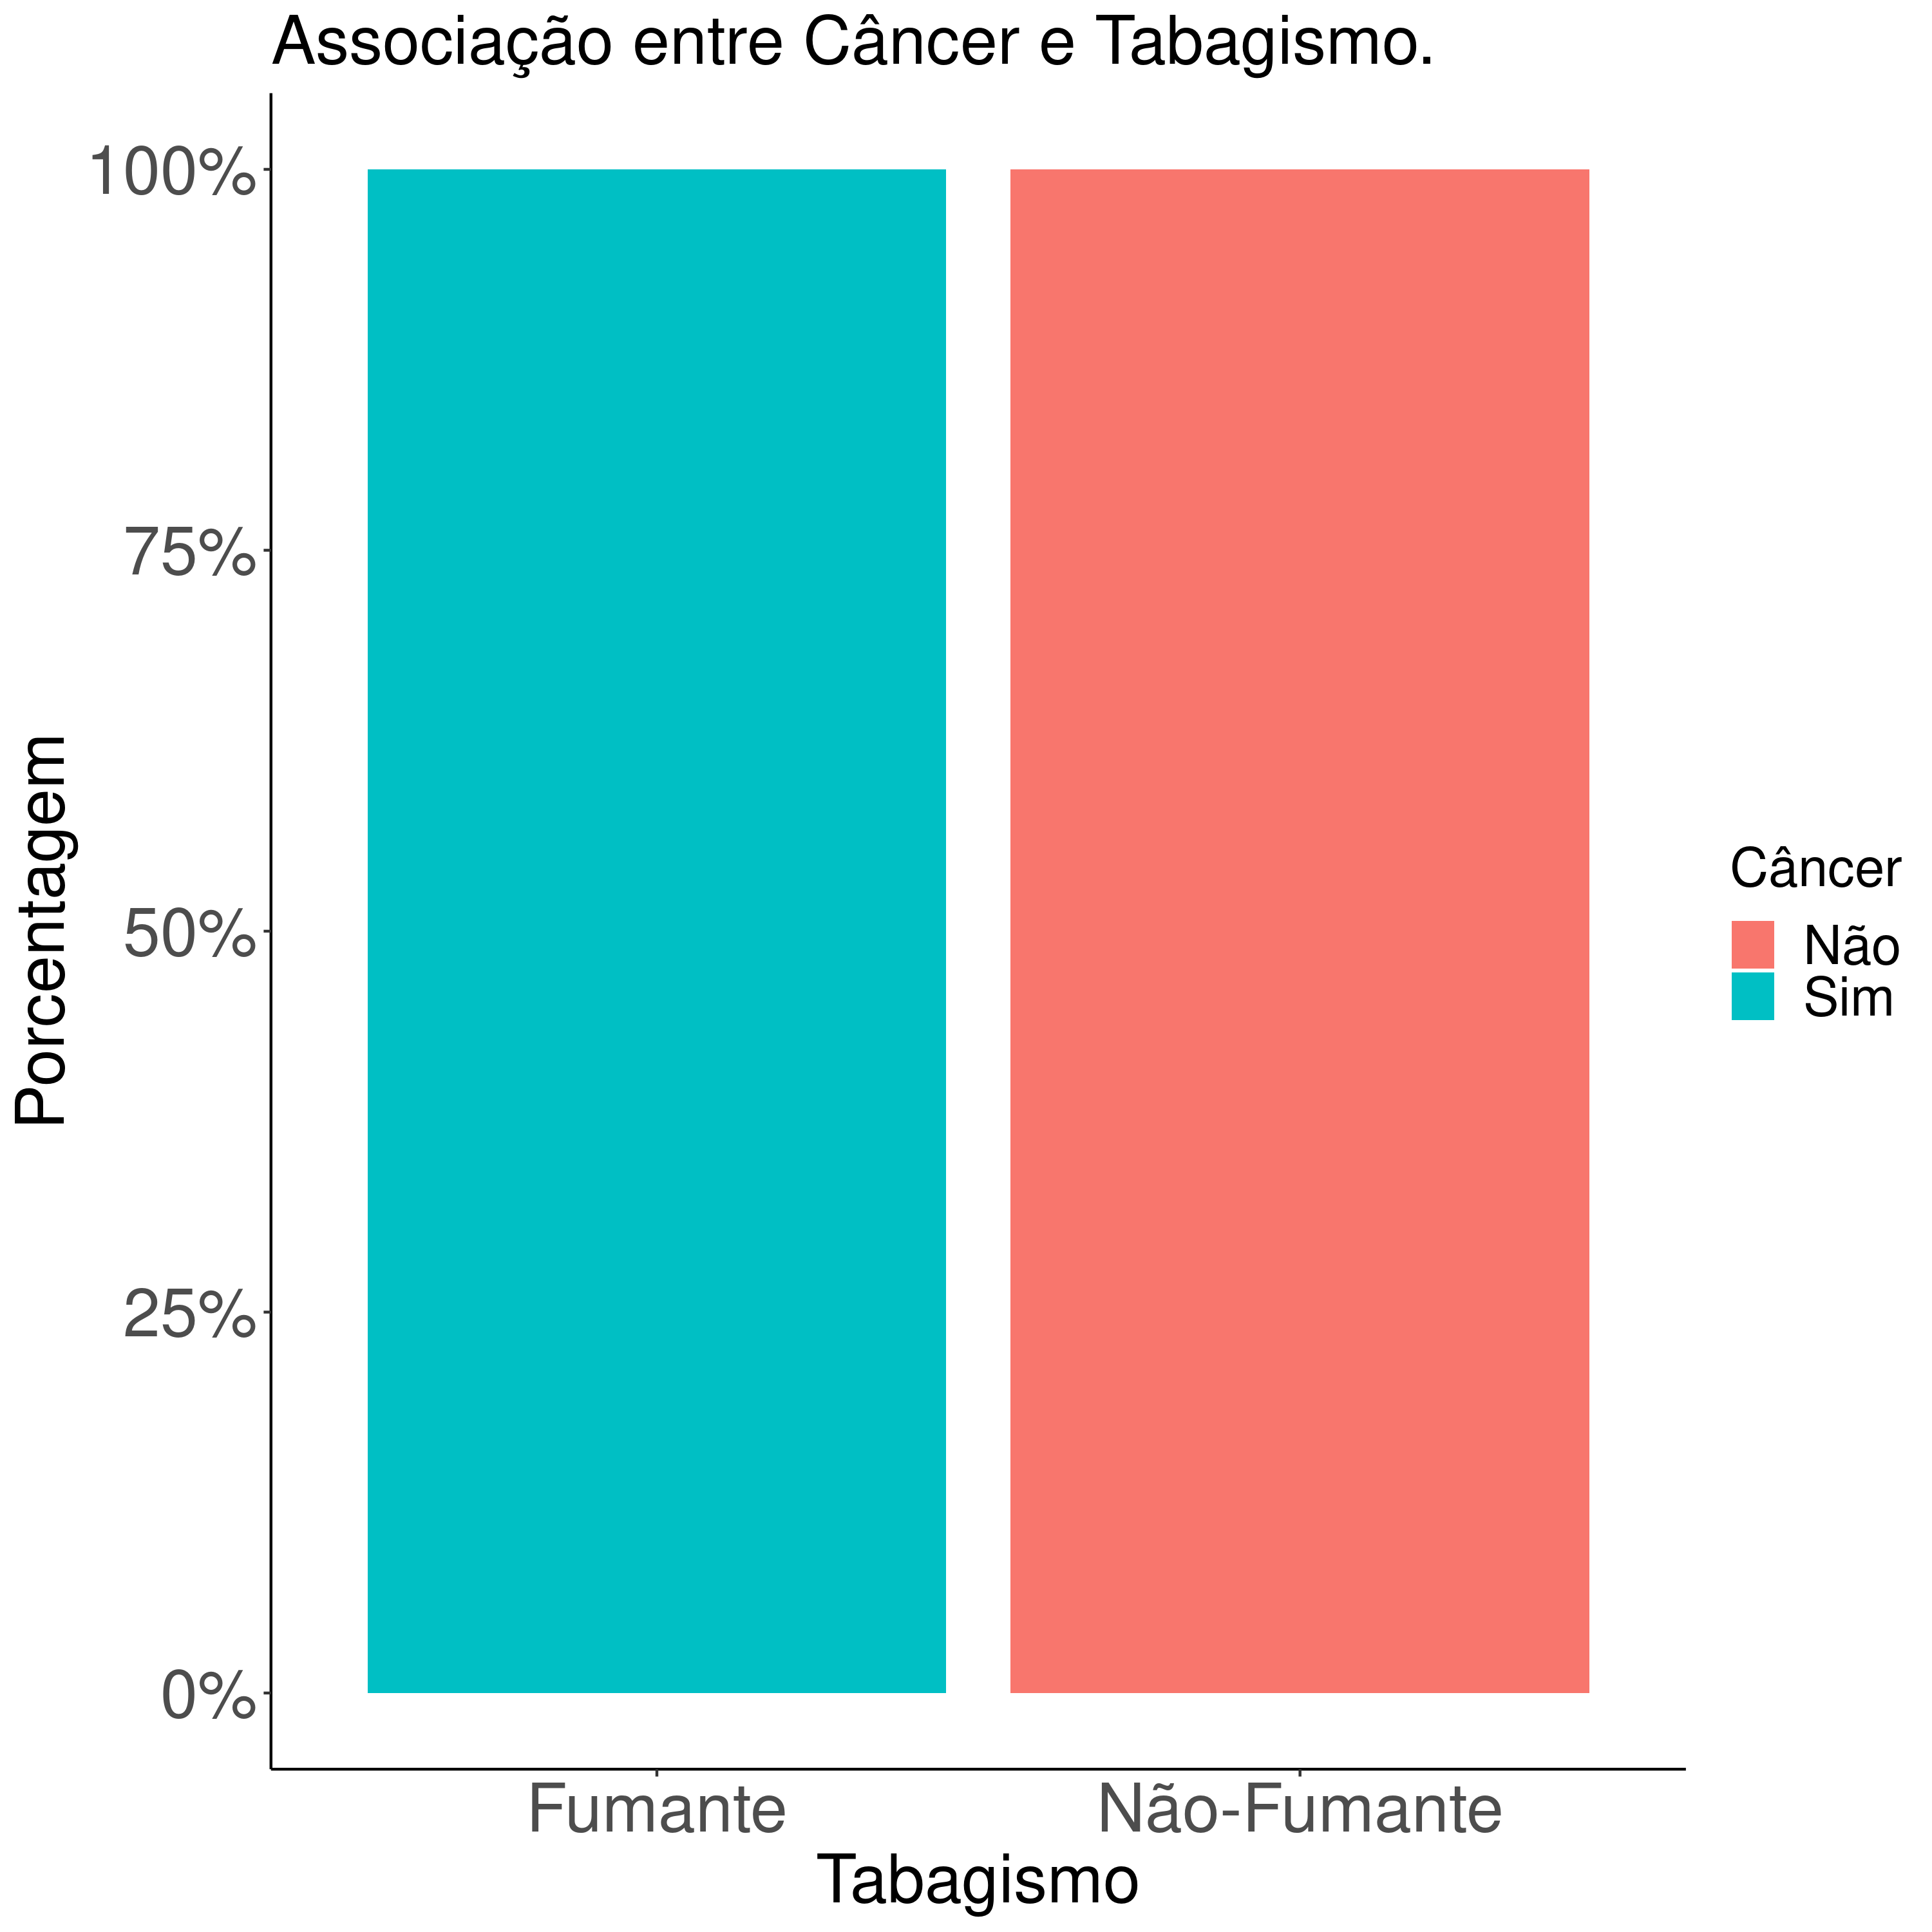
\includegraphics[width = 0.75\linewidth]{figures/associacao.png}
	\caption{Representação da Tabela~\ref{tab:associacao_rel} usando gráfico de barras.}
	\label{tab:graph-associacao}
\end{figure}
\end{frame}

\begin{frame}{Exemplo de não associação}
Um pesquisador está interessado em estudar a associação entre Gênero e Tabagismo. Para isso, ele coletou uma amostra de 300 de elementos da população e obteve a tabela contingência na Tabela~\ref{tab:nao-associacao}.
\begin{table}[htbp]
	\centering
	\caption{Tabela de contingência entre Gênero e Tabagismo.}
	\label{tab:nao-associacao}
	\begin{tabular}{l|cc|l}
		\toprule[0.05cm]
		& \multicolumn{2}{|c|}{Gênero} & \\ \cmidrule{2-3}
		Tabagismo & Homem & Mulher & Total\\ \midrule[0.05cm]
		Não-Fumante & 80 & 40 & 120\\
		Fumante & 120 & 60 & 180\\ \midrule[0.05cm]
		Total & 200 & 100 & 300\\ \bottomrule[0.05cm]
	\end{tabular}
\end{table}
\end{frame}

\begin{frame}{Exemplo de não-associação: solução}
Precisamos de uma referência e podemos calcular a frequência relativa ao total das colunas ou total das linhas. Neste exemplo, vamos usar o total das colunas.
\begin{table}[htbp]
	\centering
	\caption{Tabela de distribuição de frequência relativa ao total das colunas.}
	\label{tab:nao-associacao_rel}
	\scalebox{0.80}{
	\begin{tabular}{l|ll|l}
		\toprule[0.05cm]
		& \multicolumn{2}{|c|}{Gênero (Y)} & \\ \cmidrule{2-3}
		Tabagismo (X) & Homem & Mulher & Total\\ \midrule[0.05cm]
		Não-Fumante & {\color{brown} $\frac{80}{200}\cdot 100 = 40\%$} &  {\color{blue}$\frac{40}{100}\cdot 100 = 40\%$} & {\color{red}$\frac{120}{300}\cdot 100= 40\%$} \\
		Fumante & $\frac{120}{200}\cdot 100 = 60\%$  &  $\frac{60}{100}\cdot 100= 60\%$ &  $\frac{180}{300}\cdot 100=60\%$ \\ \midrule[0.05cm]
		Total & $\frac{200}{200}\cdot 100= 100\%$ &  $\frac{100}{100}\cdot 100 = 100\%$  & $\frac{300}{300}\cdot 100= 100\%$ \\ \bottomrule[0.05cm]
	\end{tabular}
	}
\end{table} 

Note que a probabilidade de um indivíduo ser Fumante é {\color{red} $40\%$}, mas
\begin{itemize}
	\item Se o valor de $Y$ é igual Homem, então a probabilidade do indvíduo ser Fumante é {\color{brown} $40\%$};
	\item Se o valor de $Y$ é igual Mulher, então a probabilidade do indvíduo ser Fumante é {\color{blue} $40\%$}.
\end{itemize}
\end{frame}

\begin{frame}{Exemplo de associação: solução}

\begin{figure}[htbp]
	\centering
	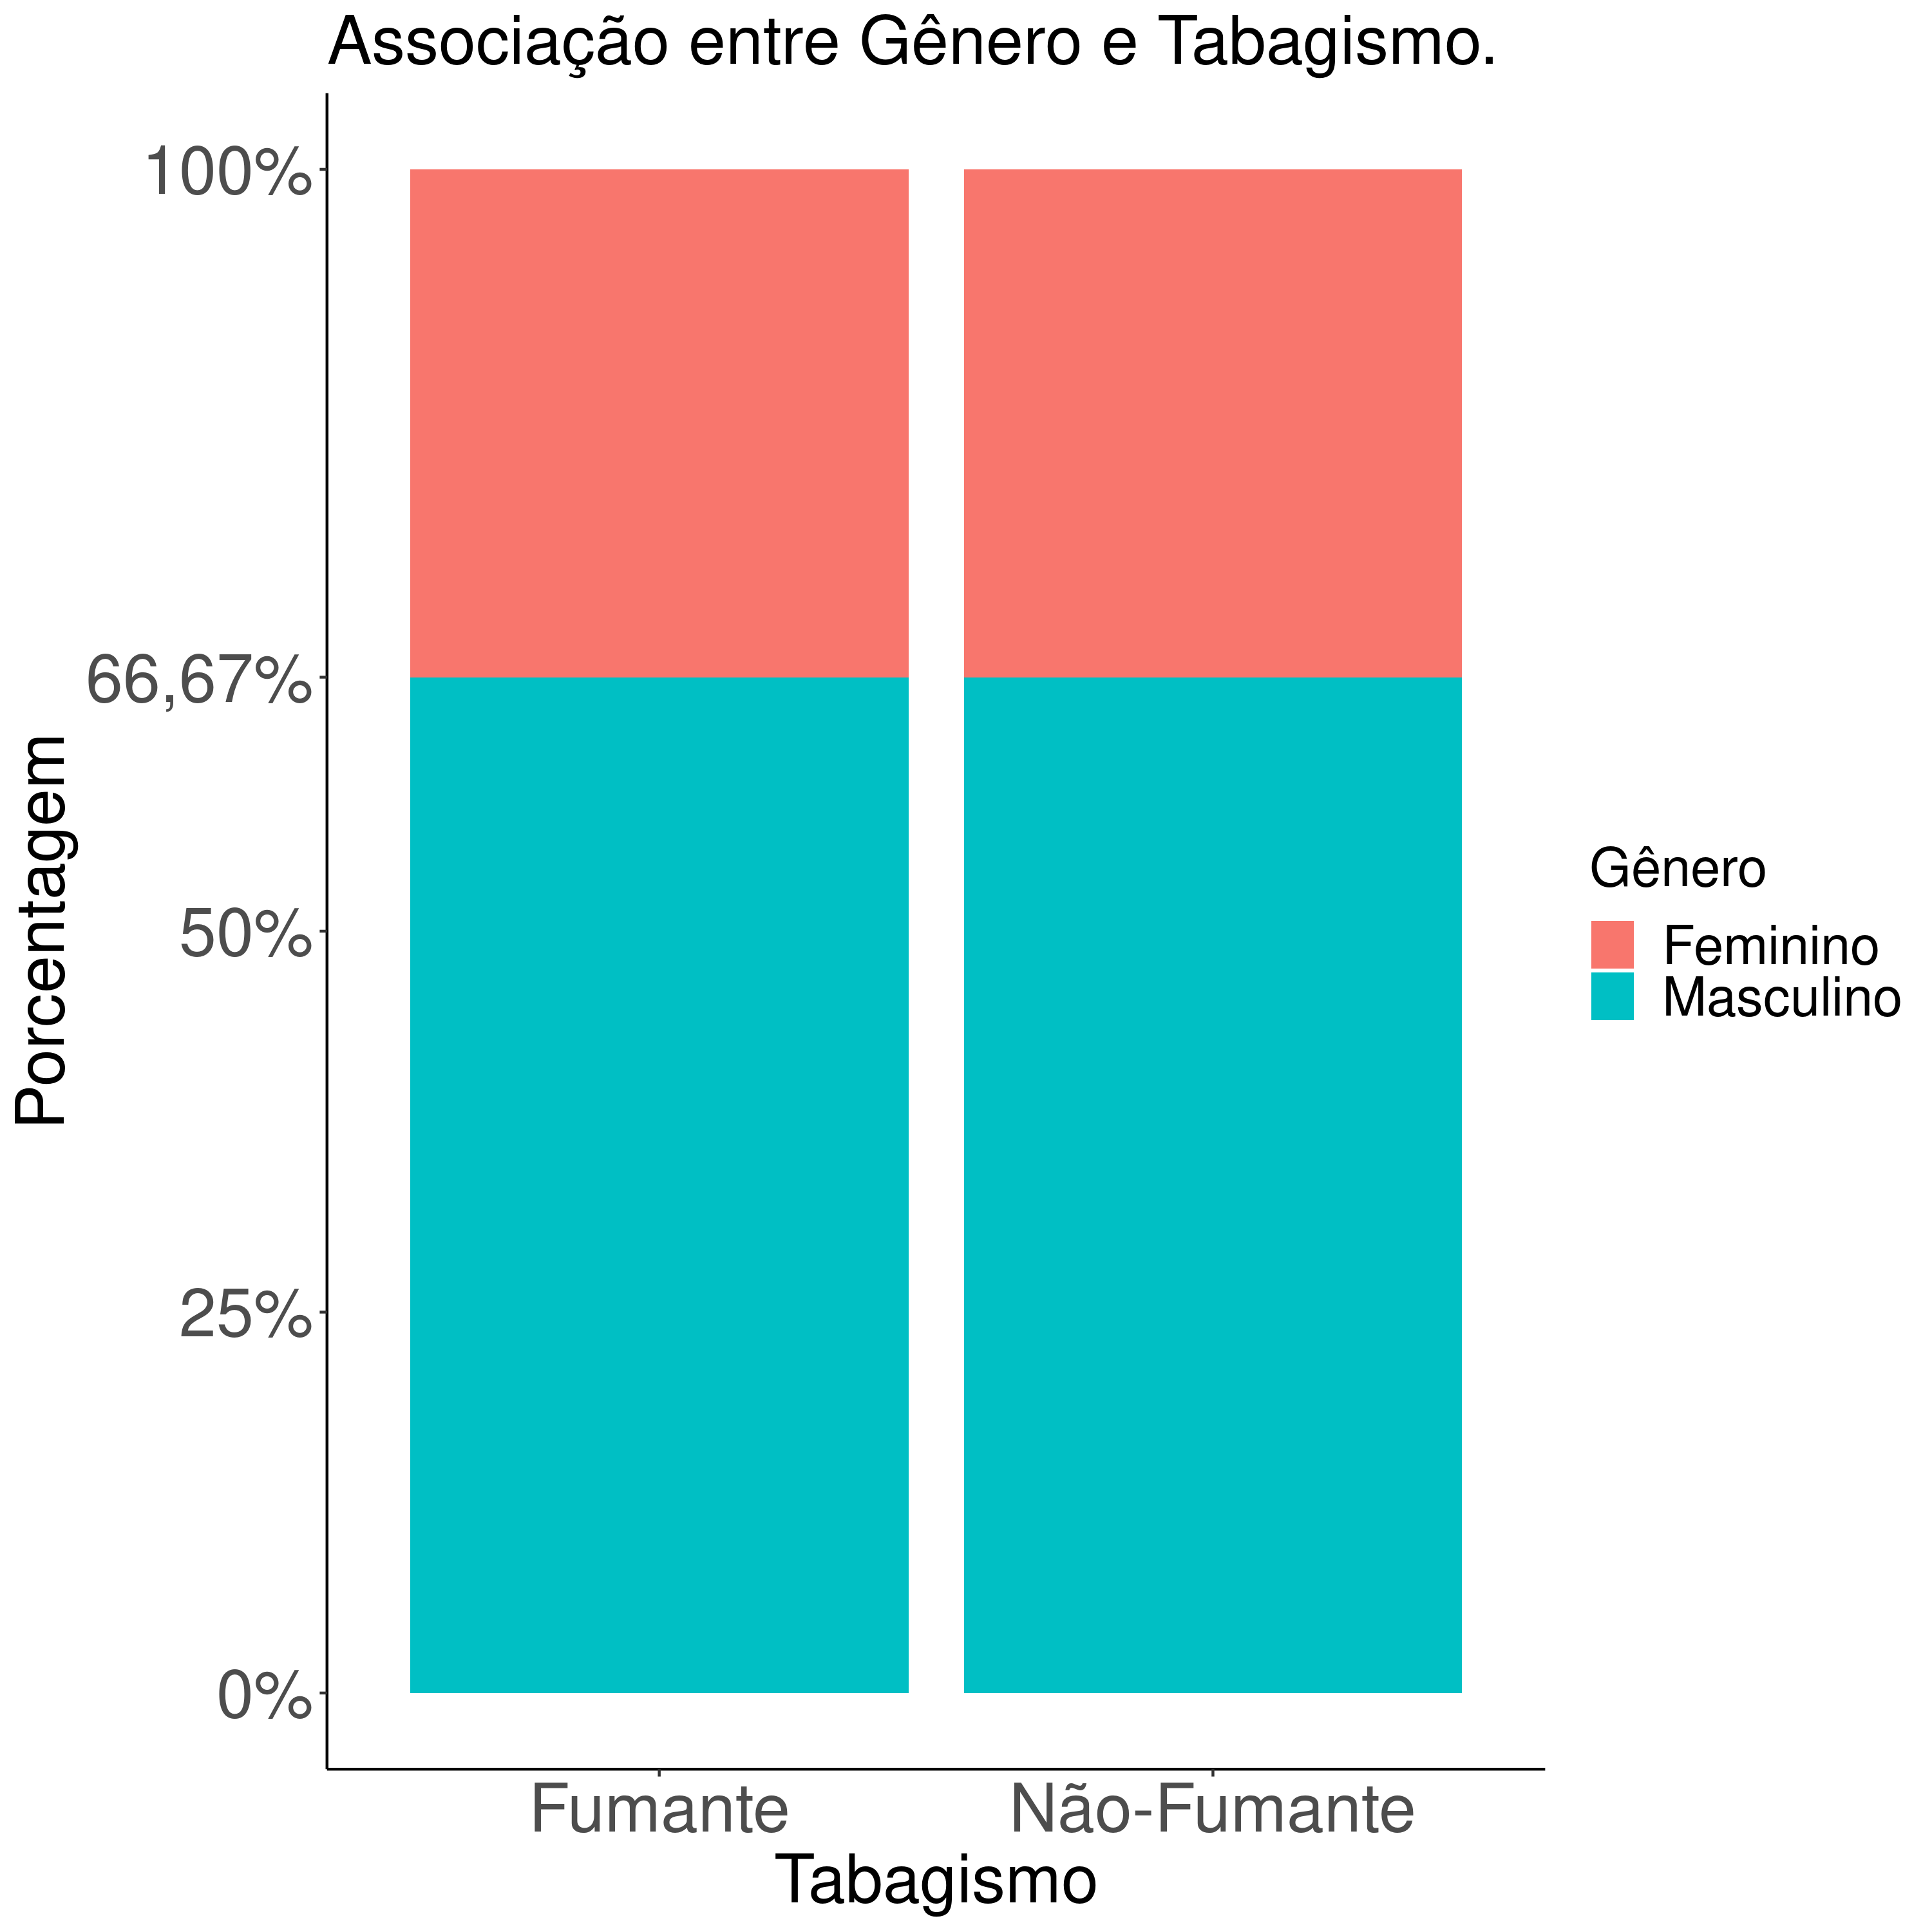
\includegraphics[width = 7cm]{figures/nao_associacao.png}
	\caption{Representação da tabela~\ref{tab:nao-associacao_rel} usando gráfico de barras.}
	\label{tab:graph-nao-associacao}
\end{figure}

\end{frame}


\begin{frame}{Propriedade de não associação}

\begin{table}[htbp]
	\centering
	\begin{minipage}{0.45\linewidth}
		\centering
		\caption{Tabela de contingência:  frequência observada.}
		\scalebox{0.65}{
		\begin{tabular}{l|cc|l}
			\toprule[0.05cm]
			& \multicolumn{2}{|c|}{Gênero} & \\ \cmidrule{2-3}
			Tabagismo & Homem & Mulher & Total\\ \midrule[0.05cm]
			Não-Fumante & 80 & 40 & 120\\
			Fumante & 120 & 60 & 180\\ \midrule[0.05cm]
			Total & 200 & 100 & 300\\ \bottomrule[0.05cm]
		\end{tabular}
		}
	\end{minipage}  
	\begin{minipage}{0.45\linewidth}
		\centering
		\caption{Tabela de contingência: frequência esperada.}
		\scalebox{0.65}{
		\begin{tabular}{l|cc|l}
			\toprule[0.05cm]
			& \multicolumn{2}{|c|}{Gênero} & \\ \cmidrule{2-3}
			Tabagismo & Homem & Mulher & Total\\ \midrule[0.05cm]
			Não-Fumante & $\frac{{\color{blue}200}\cdot {\color{brown} 120}}{{\color{red} 300}}= 80$ & $\frac{{\color{blue} 100} \cdot {\color{brown} 120}}{{\color{red} 300}}= 40$ & {\color{brown} 120}\\
			Fumante & $\frac{{\color{blue} 200} \cdot {\color{brown} 180}}{{\color{red} 300}}= 120$ & $\frac{{\color{blue} 100} \cdot {\color{brown} 180}}{{\color{red} 300}} =60$ & {\color{brown} 180}\\ \midrule[0.05cm]
			Total & {\color{blue} 200} & {\color{blue} 100} & {\color{red} 300}\\ \bottomrule[0.05cm]
		\end{tabular}
		}
	\end{minipage}
\end{table}


\vfill

{\color{red}\bf Propriedade importante:} {\color{red} No contexto de não associação, as tabelas de distribuição de frequência observada e a tabela de distribuição de frequência esperada são iguais.}

\end{frame}

\begin{frame}{Associação}
Considere um estudo exploratório que estuda a recuperação funcional de pacientes submetidos a uma certa classe de atos cirúrgicos em cinco hospitais. Os hospitais $A, B, C, D$ são hospitais comuns e o hospital $E$ é um hospital de referência que recebe hospitais mais greves. Obtemos a seguinte tabela de contingência descrita Tabela~\ref{tab:independencia_conj}. As duas variáveis estão associadas?
\begin{table}[htbp]
	\centering
	\caption{Tabela de contingência.}
	\label{tab:independencia_conj}
	\begin{tabular}{l|ccc|l}
		\toprule[0.05cm]
		& \multicolumn{3}{|c|}{Recuperação funcional} & \\ \cmidrule[0.05cm]{2-4}
		Hospital & Nenhuma & Parcial & Completa & Total \\ \midrule[0.05cm]
		$A+B+C+D$ & 47 & 120 & 118 & 285\\
		$E$ & 43 & 29 & 10 & 82 \\ \midrule[0.05cm]
		Total & 90 & 149 & 128 & 367\\ \bottomrule[0.05cm]
	\end{tabular}
\end{table}
\end{frame}

\begin{frame}{Solução}
Primeiro, vamos construir a tabela de contingência com frequência relativa em relação ao total das linhas conforme Tabela~\ref{tab:independencia_row}.
\begin{table}[htbp]
	\centering
	\caption{Tabela de contingência relativa ao total das linhas.}
	\label{tab:independencia_row}
	\begin{tabular}{l|ccc|l}
		\toprule[0.05cm]
		& \multicolumn{3}{|c|}{Recuperação funcional} & \\ \cmidrule[0.05cm]{2-4}
		Hospital & Nenhuma & Parcial & Completa & Total \\ \midrule[0.05cm]
		$A+B+C+D$ & 16,5\% & 42,1\% & 41,4\% & 100\%\\
		$E$ & 52,4\% & 35,4\% & 12,2\% & 100\% \\ \midrule[0.05cm]
		Total & 24,5\% & 40,6\% & 34,9\% & 100\%\\ \bottomrule[0.05cm]
	\end{tabular}
\end{table} 
\end{frame}

\begin{frame}{Solução}

\begin{figure}[htbp]
	\centering
	\caption{Associação entre Recuperação Funcional e Hospital.}
	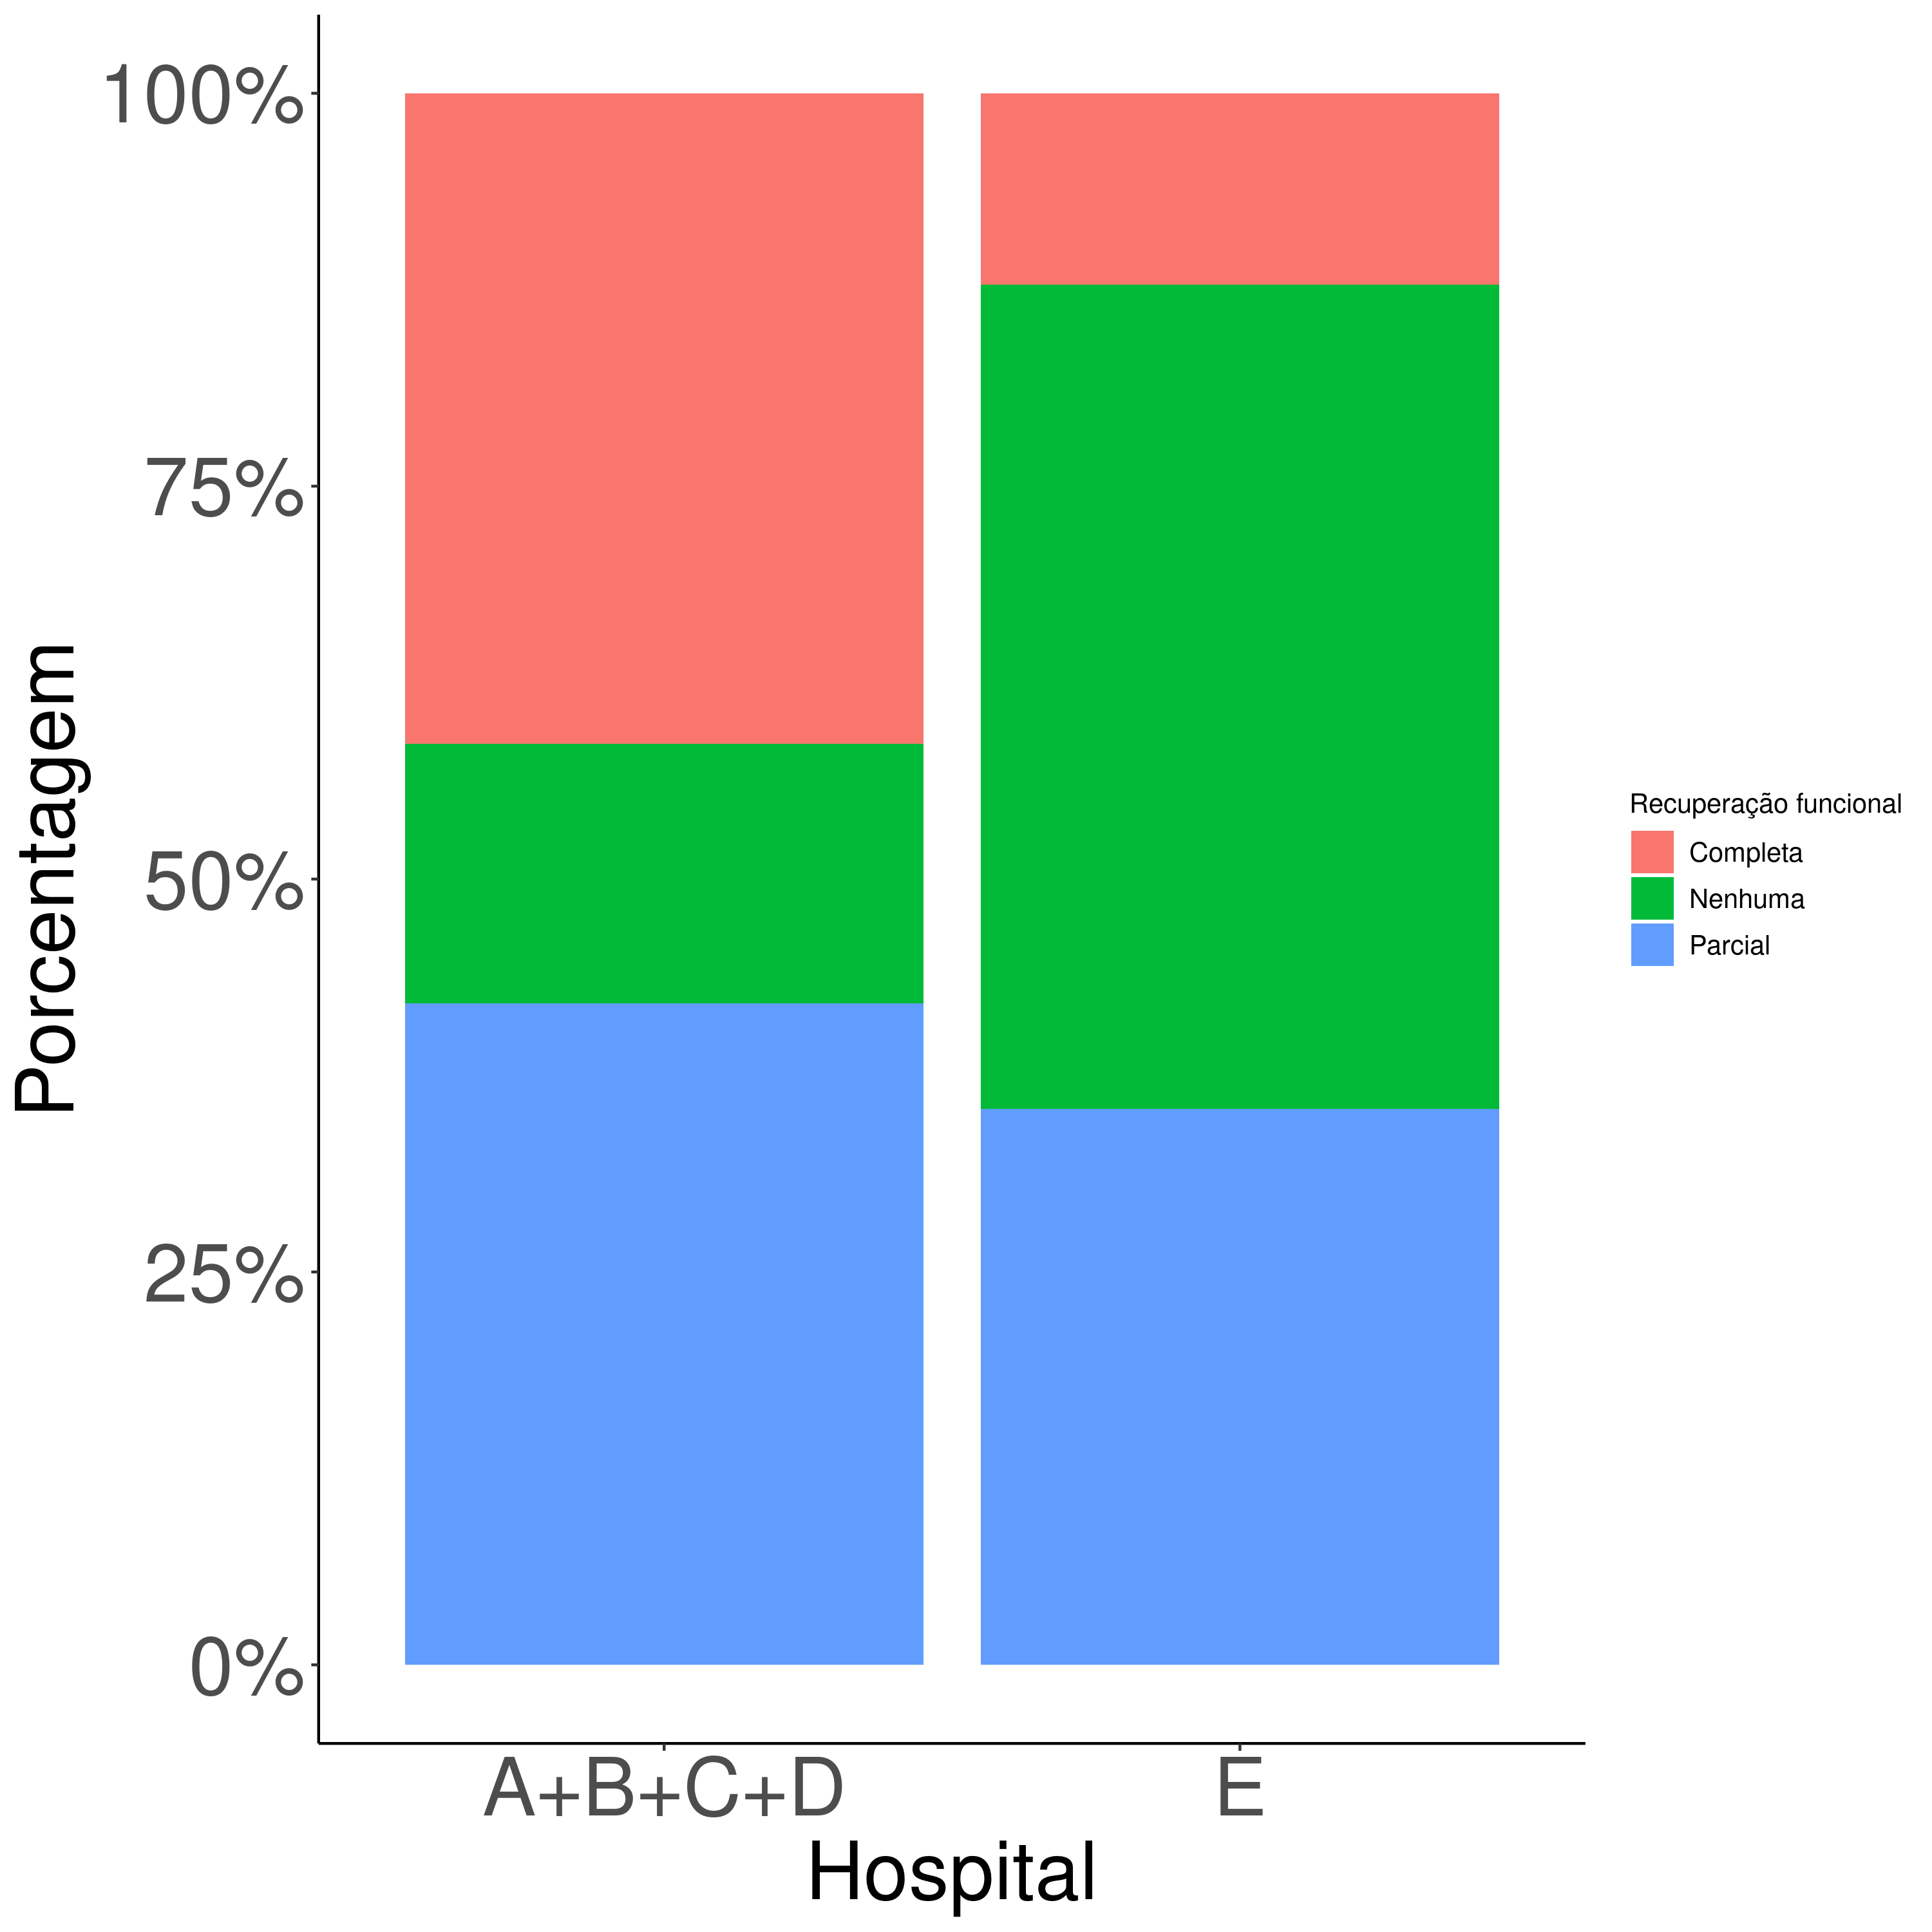
\includegraphics[width = 0.6\linewidth]{figures/associacao_moderada.png}
\end{figure}

Como as barras do gráfico de barras são diferentes, podemos afirmar que existe associação entre Recuperação Funcional e o tipo de Hospital.
\end{frame}

\begin{frame}{Teste de associação}
Considere duas variáveis qualitativas $X$ e $Y$ com valores possíveis:
\begin{itemize}
	\item $X: A_1, A_2, \cdots, A_r$;
	\item $Y: B_1, B_2, \cdots, B_s$;
\end{itemize}
com tabela de contingência conforme tabela abaixo
\begin{table}[htbp]
	\centering
	\begin{tabular}{c|cccc|c}
		\toprule[0.05cm]
		& \multicolumn{4}{|c|}{$Y$} & \\ \cmidrule[0.05cm]{2-5}
		$X$ & $B_1$ & $B_2$ & $\cdots$ & $B_s$ & Total\\ \midrule[0.05cm]
		$A_1$ & $n_{11}$ & $n_{12}$ & $\cdots$ & $n_{1s}$ & $n_{1.}$\\
		$A_2$ & $n_{21}$ & $n_{22}$ & $\cdots$ & $n_{2s}$ & $n_{2.}$\\
		$\vdots$ & $\vdots$ & $\vdots$ & $\ddots$ & $\vdots$ & $\vdots$\\
		$A_r$ & $n_{r1}$ & $n_{r2}$ & $\cdots$ & $n_{rs}$ & $n_{r.} $\\ \midrule[0.05cm]
		Total & $n_{.1}$ & $n_{.2}$ & $\cdots$ & $n_{.s}$ & $n_{..}$\\
		\bottomrule[0.05cm]
	\end{tabular}
\end{table}
em que 
\begin{itemize}
	\item $n_{i.} = n_{i1}+n_{i2}+\cdots+n_{is}, \quad i =1,2, \cdots, r$;
	\item $n_{.j} = n_{1j}+n_{2j}+\cdots+n_{rj}, \quad j =1,2, \cdots, s$;
	\item $n_{..}$ é o tamanho da amostra.
\end{itemize}

\end{frame}

\begin{frame}{Teste de associação}
Desejamos testar se $X$ e $Y$ são independentes, ao nível de significância $\alpha$.

\textbf{Passo 1)}  Vamos testar as hipóteses:
\begin{align*}
&H_0: \mbox{As duas variáveis não estão associadas};\\
&H_1: \mbox{As duas variáveis estão associadas}.
\end{align*}
\vfill

{\bf Passo 2)} Nível de significância $\alpha$ fixado pelo pesquisador.
\vfill

{\bf Passo 3)} Sob $H_0$, teríamos a tabela de contingência conforme Tabela~\ref{tab:tab_h0}.


\begin{table}[htbp]
	\centering
	\caption{Tabela de contingência sob $H_0$.}
	\label{tab:tab_h0}
	\scalebox{0.75}{
	\begin{tabular}{c|cccc}
		\toprule[0.05cm]
		& \multicolumn{4}{|c}{$Y$}  \\ \cmidrule[0.05cm]{2-5}
		$X$ & $B_1$ & $B_2$ & $\cdots$ & $B_s$ \\ \midrule[0.05cm]
		$A_1$ & $n^\star_{11}=\dfrac{n_{1.}\cdot n_{.1}}{n_{..}} $ & $n^\star_{12}=\dfrac{n_{1.}\cdot n_{.2}}{n_{..}}$ & $\cdots$ & $n^\star_{1s}=\dfrac{n_{1.}\cdot n_{.s}}{n_{..}}$ \\
		$A_2$ & $n^\star_{21}=\dfrac{n_{2.}\cdot n_{.1}}{n_{..}}$ & $n^\star_{22}=\dfrac{n_{2.}\cdot n_{.2}}{n_{..}}$ & $\cdots$ & $n^\star_{2s}=\dfrac{n_{2.}\cdot n_{.s}}{n_{..}}$ \\
		$\vdots$ & $\vdots$ & $\vdots$ & $\ddots$ & $\vdots$ \\
		$A_r$ & $n^\star_{r1}=\dfrac{n_{r.}\cdot n_{.1}}{n_{..}}$ & $n^\star_{r2}=\dfrac{n_{r.}\cdot n_{.2}}{n_{..}}$ & $\cdots$ & $n^\star_{rs}=\dfrac{n_{r.}\cdot n_{.s}}{n_{..}}$ \\ 
		\bottomrule[0.05cm]
	\end{tabular}
	}
\end{table}

\end{frame}


\begin{frame}{Teste de associação}

\scriptsize
{\bf Passo 3) (continuação)} Se $X$ e $Y$ são independentes (sob $H_0$), temos que $n^\star_{ij}=n_{ij}, \quad i=1,\dots, r,j=1,\dots, s$. Note que se,
\begin{itemize}
	\item Se as distâncias $\dfrac{(n_{ij}-n^\star_{ij})^2}{n^\star{ij}}$ forem pequenas, decidimos por $H_0$;
	\item Se as distâncias $\dfrac{(n_{ij}-n^\star_{ij})^2}{n^\star{ij}}$ forem grandes, decidimos por $H_1$;
\end{itemize}
então calculamos uma medida chamada qui-quadrado 
\begin{align*}
\chi^2 &= \dfrac{(n_{11} - n^\star_{11})^2}{n^\star_{11}} + \dfrac{(n_{12} - n^\star_{12})^2}{n^\star_{12}} + \cdots + \dfrac{(n_{1s} - n^\star_{1s})^2}{n^\star_{1s}} + \\
&+ \dfrac{(n_{21} - n^\star_{21})^2}{n^\star_{21}} + \dfrac{(n_{22} - n^\star_{22})^2}{n^\star_{22}} + \cdots + \dfrac{(n_{2s} - n^\star_{2s})^2}{n^\star_{2s}} + \\
&\vdots\\
&+\dfrac{(n_{r1} - n^\star_{r1})^2}{n^\star_{r1}} + \dfrac{(n_{r2} - n^\star_{r2})^2}{n^\star_{r2}} + \cdots + \dfrac{(n_{rs} - n^\star_{rs})^2}{n^\star_{rs}},
\end{align*}
e
\begin{itemize}
	\item Se $\chi^2$ for pequeno ($\chi^2 \leq x_c$), decidimos por $H_0$;
	\item Se $\chi^2$ for grande ($\chi^2 > x_c$), decidimos por $H_1$;
\end{itemize}
e a região crítica é da forma $RC= \{\chi^2 \mid \chi^2 > x_c \}$.
	
\normalsize
\end{frame}

\begin{frame}{Teste de associação}


{\bf Passo 4)} Pode-se provar que $\chi^2$ tem distribuição qui-quadrado com $(r-1)\cdot (s-1)$ graus de liberdade. 

Precisamos achar o valor crítico:
\begin{align*}
\alpha &= P(H_1 \mid H_0)= P(\chi_{(r-1)\cdot (s-1)}^2 > \chi^2_{1-\alpha;(r-1)\cdot (s-1)} \mid H_0)\\
&= 1 - P(\chi^2 \leq \chi^2_{1-\alpha;(r-1)\cdot (s-1)})
\end{align*}
e $P(\chi^2 \leq \chi^2_{1-\alpha;(r-1)\cdot (s-1)}) = 1 - \alpha$.
\vfill

{\bf Passo 5)} Verificar se a $\chi^2 \in RC$ para decidir entre $H_0$ e $H_1$.
\vfill

{\bf Valor-p} Suponha que o valor de qui-quadrado seja $Q$ e seja $X$ uma variável aleatória com distribuição qui-quadrado com $(r-1)\cdot (s-1)$ graus de liberdade. Calculamos o p-valor através 
\begin{align*}
p = P(X > \chi^2 \mid H_0) = 1 - P(\chi_{(r-1)\cdot (s-1)}^2 \leq \chi^2).
\end{align*}

\end{frame}

\begin{frame}{Teste de associação}

\begin{block}{Exemplo}
Considere um estudo exploratório que estuda a recuperação funcional de pacientes submetidos a uma certa classe de atos cirúrgicos em cinco hospitais. Os hospitais $A, B, C, D$ são hospitais comuns e o hospital $E$ é um hospital de referência que recebe hospitais mais greves. Obtemos a seguinte tabela de contingência conforme Tabela~\ref{tab:independencia}. As duas variáveis estão associadas ao nível de 5\%?
\begin{table}[htbp]
	\centering
	\caption{Tabela de distribuição de frequênia conjunta.}
	\label{tab:independencia}
	\begin{tabular}{l|ccc|l}
		\toprule[0.05cm]
		& \multicolumn{3}{|c|}{Recuperação funcional} & \\ \cmidrule[0.05cm]{2-4}
		Hospital & Nenhuma & Parcial & Completa & Total \\ \midrule[0.05cm]
		$A+B+C+D$ & 47 & 120 & 118 & 285\\
		$E$ & 43 & 29 & 10 & 82 \\ \midrule[0.05cm]
		Total & 90 & 149 & 128 & 367\\ \bottomrule[0.05cm]
	\end{tabular}
\end{table}	
\end{block}

\end{frame}


\begin{frame}{Teste de associação}

\normalsize
\begin{block}{Solução}
	{\bf Passo 1)} Desejamos testar as seguintes hipóteses
	\begin{itemize}
		\item $H_0:$ as duas variáveis não são associadas;
		\item $H_1:$ as duas variáveis estão associadas.
	\end{itemize}
	\vfill
	
	{\bf Passo 2)} Nível de significância $\alpha = 0,01.$
	\vfill
	
	{\bf Passo 3)} Rejeitamos $H_0$ se $\chi^2$ for grande. Ou seja,
	$RC = \{ \chi^2 \mid \chi^2 > \chi^2_{1-\alpha;(r-1)\cdot (s-1)} \}.$
	\vfill
	
	{\bf Passo 4)} Vamos encontrar o valor crítico:
	\begin{itemize}
		\item $P\left( \chi_{(r-1)\cdot (s-1)}^2 \leq \chi^2_{1-\alpha;(r-1)\cdot (s-1)} \right) =  P\left( \chi_{(2-1)\cdot (3-1)}^2 \leq \chi^2_{1-\alpha;(r-1)\cdot (s-1)} \right) = \allowbreak 1 -\alpha = 0,99$, então $\chi^2_{0,99;2} = 9,2103404 $
	\end{itemize}

\end{block}
\normalsize

\end{frame}

\begin{frame}{Teste de associação}

\small
	{\bf Passo 5)}
	Agora calculamos a tabela de contingência esperada.
	\begin{table}[htbp]
		\centering
		\caption{Tabela de contingência esperada.}
		\label{tab:esperada}
		\begin{tabular}{l|ccc|l}
			\toprule[0.05cm]
			& \multicolumn{3}{|c|}{Recuperação funcional} & \\ \cmidrule[0.05cm]{2-4}
			Hospital & Nenhuma & Parcial & Completa & Total \\ \midrule[0.05cm]
			$A+B+C+D$ & $\frac{90\cdot 285}{367} = 69,89$ & $\frac{149\cdot 285}{367}= 115,71$  & $\frac{128\cdot 285}{367} =99,40$  & 185\\
			$E$ & $\frac{90\cdot 82}{367} = 20,11$ & $\frac{149 \cdot 82}{367} = 33,29$ & $\frac{128 \cdot 82}{367} = 28,60$ & 82 \\ \midrule[0.05cm]
			Total & 90 & 149 & 128 & 367\\ \bottomrule[0.05cm]
		\end{tabular}
	\end{table}
	Então o $\chi^2$ é 
	\begin{align*}
	\chi^2 &= \dfrac{(47-69,89)^2}{69,89} + \dfrac{(115,71-120)^2}{115,71} + \dfrac{(99,40-118)^2}{99,40}+\\
	&+ \dfrac{(20,11-43)^2}{20,11} + \dfrac{(29-33,29)^2}{33,29} + \dfrac{(28,60-10)^2}{28,60} = 49,84.
	\end{align*}
	
	Como $\chi^2 = 49,84 > \chi^2_{0,99;2} = 9,2103404$, então $\chi^2 \in RC$ e rejeitamos $H_0$.
	\vfill
	
	Então, ao nível de significância $1\%$, o tipo de hospital e a recuperação estão associadas.
	
\normalsize
\end{frame}

\begin{frame}{Teste de associação}

\begin{block}{Solução (valor-p)}
	O  valor-p é dado por
	\begin{align*}
		p &= P \left( \chi^2 > \chi^2_{obs} \mid H_0 \right) = 1 - P \left( \chi^2_{(r-1)\cdot (s-1)} \leq \chi^2_{obs} \right),
	\end{align*}
	em que $\chi^2_{obs}$ é o valor observado da medida qui-quadrado da amostra.
	
	Note que $\chi^2_{obs} = 49,84$, então o valor-p é dado por
	\begin{align*}
		p &= 1 - P \left( \chi^2_{(r-1)\cdot (s-1)} \leq \chi^2_{obs} \right)\\
		&= 1 - P \left( \chi_{2}^2 \leq 49,84 \right)\\
		&= 1 - 1\\
		&= 0.
	\end{align*}
	
	Como $p = 0 < \alpha = 0,01$, e rejeitamos $H_0$. Ou seja, ao nível de significância $\alpha=0,01$, as duas variáveis qualitativas estão associadas. 
\end{block}

\end{frame}

\subsection{Poder e tamanho da amostra.}

\begin{frame}{Poder do teste: $H_0:\mbox{Não existe associação}$ e $H_1:\mbox{Existe associação} $.}

\normalsize

Imagine que
\begin{itemize}
	\item Hipóteses: $H_0:\mbox{Não existe associação}$ e $H_1:\mbox{Existe associação} $;
	\item $H_1$ é verdade e $\lambda = \chi^2_{obs}$. Considere $w^2 = \frac{\chi^2}{n}$ e $n$ é o tamanho da amostra. $w$ é chamado de \textit{effect size};
	\item $\chi^2  \sim \chi^2_{(r-1)\cdot (s-1)}\left( \lambda \right)$;
	\item Ao nível de significância $\alpha$, temos $RC = \{ \chi^2 \mid \chi^2 > \chi^2_{1-\alpha; (r-1) \cdot (s-1)}  \}$.
\end{itemize}
\vfill	

Poder do teste é dado
\begin{align*}
\textcolor{important}{1-\beta} &=1 - \left[P\left(  \chi^2 \leq \chi_{1-\alpha; (r-1)\cdot (s-1)}^2 \mid H_1 \right)\right]\\
&= 1 - P\left( \chi_{(r-1)\cdot (s-1)}^2(\lambda) \leq \chi_{1-\alpha; (r-1)\cdot (s-1)}^2 \right).
\end{align*}
A \textcolor{important}{Função Poder}, dado o tamanho da amostra $n$, é uma função das médias populacionais na hipótese alternativa  $\pi: (0, \infty) \longrightarrow [0,1]$ dada por
\begin{align*}
\pi(\lambda) = 1 - P\left( \chi_{(r-1)\cdot (s-1)}^2(\lambda) \leq \chi_{1-\alpha; (r-1)\cdot (s-1)}^2 \right), \lambda \in (0, \infty).
\end{align*}
Alguns livros chamam a Função Poder de \textcolor{important}{Curva de Característica Operacional.}

\normalsize

\end{frame}


\begin{frame}{Tamanho da amostra: $H_0:\mbox{Não existe associação}$ e $H_1:\mbox{Existe associação} $.}

Imagine que
\begin{itemize}
	\item Hipóteses: $H_0:\mbox{Não existe associação}$ e $H_1:\mbox{Existe associação} $;
	\item $H_1$ é verdade e $\lambda = \chi^2_{obs}$. Chamamos $w = \sqrt{\frac{\chi^2}{n}}$ de \textit{effect size} e $n$ é o tamanho da amostra;
	\item $\chi^2  \sim \chi^2_{(r-1)\cdot (s-1)}\left( \lambda \right)$;
	\item Ao nível de significância $\alpha$, temos $RC = \{ \chi^2 \mid \chi^2 > \chi^2_{1-\alpha; (r-1) \cdot (s-1)}  \}$.
\end{itemize}
\vfill

Considere $1-\beta$, $\alpha$, $n$, $r = $ número de linhas e $s$ = número de colunas, então o tamanho \sout{mínimo} da amostra é solução da seguinte equação
\begin{align*}
1-\beta = 1 - P\left( \chi_{(r-1)\cdot (s-1)}^2(\lambda) \leq \chi_{1-\alpha; (r-1)\cdot (s-1)}^2 \right),
\end{align*}
em que $\lambda = n \cdot w^2$. Geralmente, usamos
\begin{itemize}
	\item $w=0,1$ para detectar uma associação fraca;
	\item $w=0,3$ para detectar uma associação moderada;
	\item $w=0,5$ para detectar uma associação forte.
\end{itemize}
Ideal seria calcular $w$ através de uma amostra piloto ou obtê-lo usando um sistema publicado e validado com a mesma população \sout{ou uma população similar}.
\end{frame}

\begin{frame}{Poder do teste: $H_0:\mbox{Não existe associação}$ e $H_1:\mbox{Existe associação} $.}

\large
\begin{block}{Exemplo}
	Considere um estudo exploratório que analisará a associação entre recuperação funcional-- Nenhuma, Parcial e Completa -- de pacientes submetidos a uma certa classe de atos cirúrgicos e o tipo de hospital. Os hospitais $A, B, C, D$ são hospitais comuns e o hospital $E$ é um hospital de referência que recebe hospitais mais greves. De um estudo piloto, sabemos que $w= 0,3$. O pesquisador planeja acompanhar $n=400$ pacientes. Qual o poder do teste ao nível de significância $\alpha=5\%$?
\end{block}
\normalsize

\end{frame}

\begin{frame}[fragile]{Poder do teste: $H_0:\mbox{Não existe associação}$ e $H_1:\mbox{Existe associação} $.}

\scriptsize
\begin{block}{Solução}
	\textbf{Passo 1)} Queremos testar as seguintes hipóteses:
	\begin{itemize}
		\item $H_0:$ recuperação funcional e o tipo de hospital não estão associadas;
		\item $H_1:$ recuperação funcional e o tipo de hospital estão associadas.
	\end{itemize}

	\textbf{Passo 2)} Nível de significância $\alpha=5\%$;
	
	\textbf{Passo 3)} Rejeitamos $H_0$ se $\chi^2$ for grande. Ou seja, $RC =\left\{ \chi^2 \mid \chi^2 > \chi^2_{1-\alpha; (r-1)\cdot (s-1)} \right\}$;
	
	\textbf{Passo 4)} Vamos encontrar o valor críticos:
	\begin{itemize}
		\item $P\left( \chi^2_{(r-1)\cdot (s-1)} \leq \chi^2_{1-\alpha;(r-1)\cdot (s-1)} \right) = P\left( \chi^2_{(2-1)\cdot (3-1)} \leq \chi^2_{0,95;(2-1)\cdot (3-1)} \right) = \allowbreak 1-\alpha=0,95$, então $\chi^2_{0,95;2} = 5,9914645$.
	\end{itemize}

	Como $n=400$, $r=2$, $s=3$, $w=0,3$ e $\lambda = n \cdot w^2 = 400 \cdot 0,3^2 = 36$, então o poder do teste é dado por
	\begin{align*}
		1-\beta &= 1 - P\left( \chi_{(r-1)\cdot (s-1)}^2(\lambda) \leq \chi_{1-\alpha; (r-1)\cdot (s-1)}^2 \right)\\
		&= 1 - P\left( \chi_{2}^2(36) \leq \chi_{0,95; 2}^2 \right) = 1 - P\left( \chi_{2}^2(36) \leq 5,9914645 \right) = 0,9999.
	\end{align*}
\end{block}

\begin{lstlisting}[language = C, caption = Código no R.]
pwr_chisq_test_association(es = 0.3, nrow = 2, ncol = 3, n = 400,
		pwr = NULL, sig_level = 0.05)
\end{lstlisting}

\normalsize

\end{frame}

\begin{frame}{Tamanho da amostra: $H_0:\mbox{Não existe associação}$ e $H_1:\mbox{Existe associação} $.}

\large
\begin{block}{Exemplo}
	Considere um estudo exploratório que analisará a associação entre recuperação funcional-- Nenhuma, Parcial e Completa -- de pacientes submetidos a uma certa classe de atos cirúrgicos e o tipo de hospital. Os hospitais $A, B, C, D$ são hospitais comuns e o hospital $E$ é um hospital de referência que recebe hospitais mais greves. De um estudo piloto, sabemos que $w= 0,3$. Dado um poder de teste $99\%$, precisamos acompanhar quantos pacientes? Use $\alpha=5\%$.
\end{block}
\normalsize

\end{frame}

\begin{frame}[fragile]{Tamanho da amostra: $H_0:\mbox{Não existe associação}$ e $H_1:\mbox{Existe associação} $.}

\scriptsize
\begin{block}{Solução}
	\textbf{Passo 1)} Queremos testar as seguintes hipóteses:
	\begin{itemize}
		\item $H_0:$ recuperação funcional e o tipo de hospital não estão associadas;
		\item $H_1:$ recuperação funcional e o tipo de hospital estão associadas.
	\end{itemize}
	
	\textbf{Passo 2)} Nível de significância $\alpha=5\%$;
	
	\textbf{Passo 3)} Rejeitamos $H_0$ se $\chi^2$ for grande. Ou seja, $RC =\left\{ \chi^2 \mid \chi^2 > \chi^2_{1-\alpha; (r-1)\cdot (s-1)} \right\}$;
	
	\textbf{Passo 4)} Vamos encontrar o valor críticos:
	\begin{itemize}
		\item $P\left( \chi^2_{(r-1)\cdot (s-1)} \leq \chi^2_{1-\alpha;(r-1)\cdot (s-1)} \right) = P\left( \chi^2_{(2-1)\cdot (3-1)} \leq \chi^2_{0,95;(2-1)\cdot (3-1)} \right) = \allowbreak 1-\alpha=0,95$, então $\chi^2_{0,95;2} = 5,9914645$.
	\end{itemize}
	
	Como $1-\beta=0,99$, $r=2$, $s=3$, $w=0,3$ e $\lambda = n \cdot w^2 = n \cdot 0,3^2$, então o poder do teste é dado por
	\begin{align*}
	1-\beta &= 0,99 = 1 - P\left( \chi_{(r-1)\cdot (s-1)}^2(n \cdot w^2) \leq \chi_{1-\alpha; (r-1)\cdot (s-1)}^2 \right)\\
	&= 1 - P\left( \chi_{2}^2(n \cdot 0,3^2) \leq \chi_{0,95; 2}^2 \right) = 1 - P\left( \chi_{2}^2(n \cdot 0,3^2) \leq 5,9914645 \right)
	\end{align*}
\end{block}
Então, precisamos acompanhar $n=238$ pacientes.

\begin{lstlisting}[language = C, caption = Código no R.]
pwr_chisq_test_association(es = 0.3, nrow = 2, ncol = 3, n = NULL,
		pwr = 0.99, sig_level = 0.05)
\end{lstlisting}
\normalsize

\end{frame}

\section{Associação entre variáveis quantitativas}

\begin{frame}{Associação entre variáveis quantitativas.}

\scriptsize
\begin{block}{Objetivo}
	Checar a associação entre duas variáveis  quantitativas estão associadas, usando:
	\begin{itemize}
		\item gráfico de dispersão;
		\item coeficiente de correlação linear de Pearson;
		\item teste de associação;
		\item Intervalo de confiança para o coeficiente de correção linear de Pearson.
	\end{itemize}
\end{block}


\begin{block}{Exemplo}
	Considere uma amostra com 10 funcionários e suponha que coletamos duas variáveis:
	\begin{itemize}
		\item $X$: Anos de serviços;
		\item $Y$: Número de clientes.
	\end{itemize}
	Os dados estão mostrados na Tabela~\ref{tab:positiva}.
		\begin{table}[ht]
		\centering
		\scalebox{0.75}{
		\begin{tabular}{c|c|c}
			\toprule[0.05cm]
			Agente & Anos de serviço ($X$) & Número de clientes ($Y$)\\ 
			\midrule[0.05cm]
			A & 2 & 48 \\ 
			B & 3 & 50 \\ 
			C & 4 & 56 \\ 
			D & 5 & 52 \\ 
			E & 4 & 43 \\ 
			F & 6 & 60 \\ 
			G & 7 & 62 \\ 
			H & 8 & 58 \\ 
			I & 8 & 64 \\ 
			J & 10 & 72 \\ 
			\bottomrule[0.05cm]
		\end{tabular}
		}
		\caption{Amostra de 10 corretores de seguros.} 
		\label{tab:positiva}
	\end{table}
\end{block}
\normalsize
\end{frame}


\begin{frame}{Associação entre variáveis quantitativas}

\begin{block}{Solução}
	\begin{figure}[htbp]
		\centering
		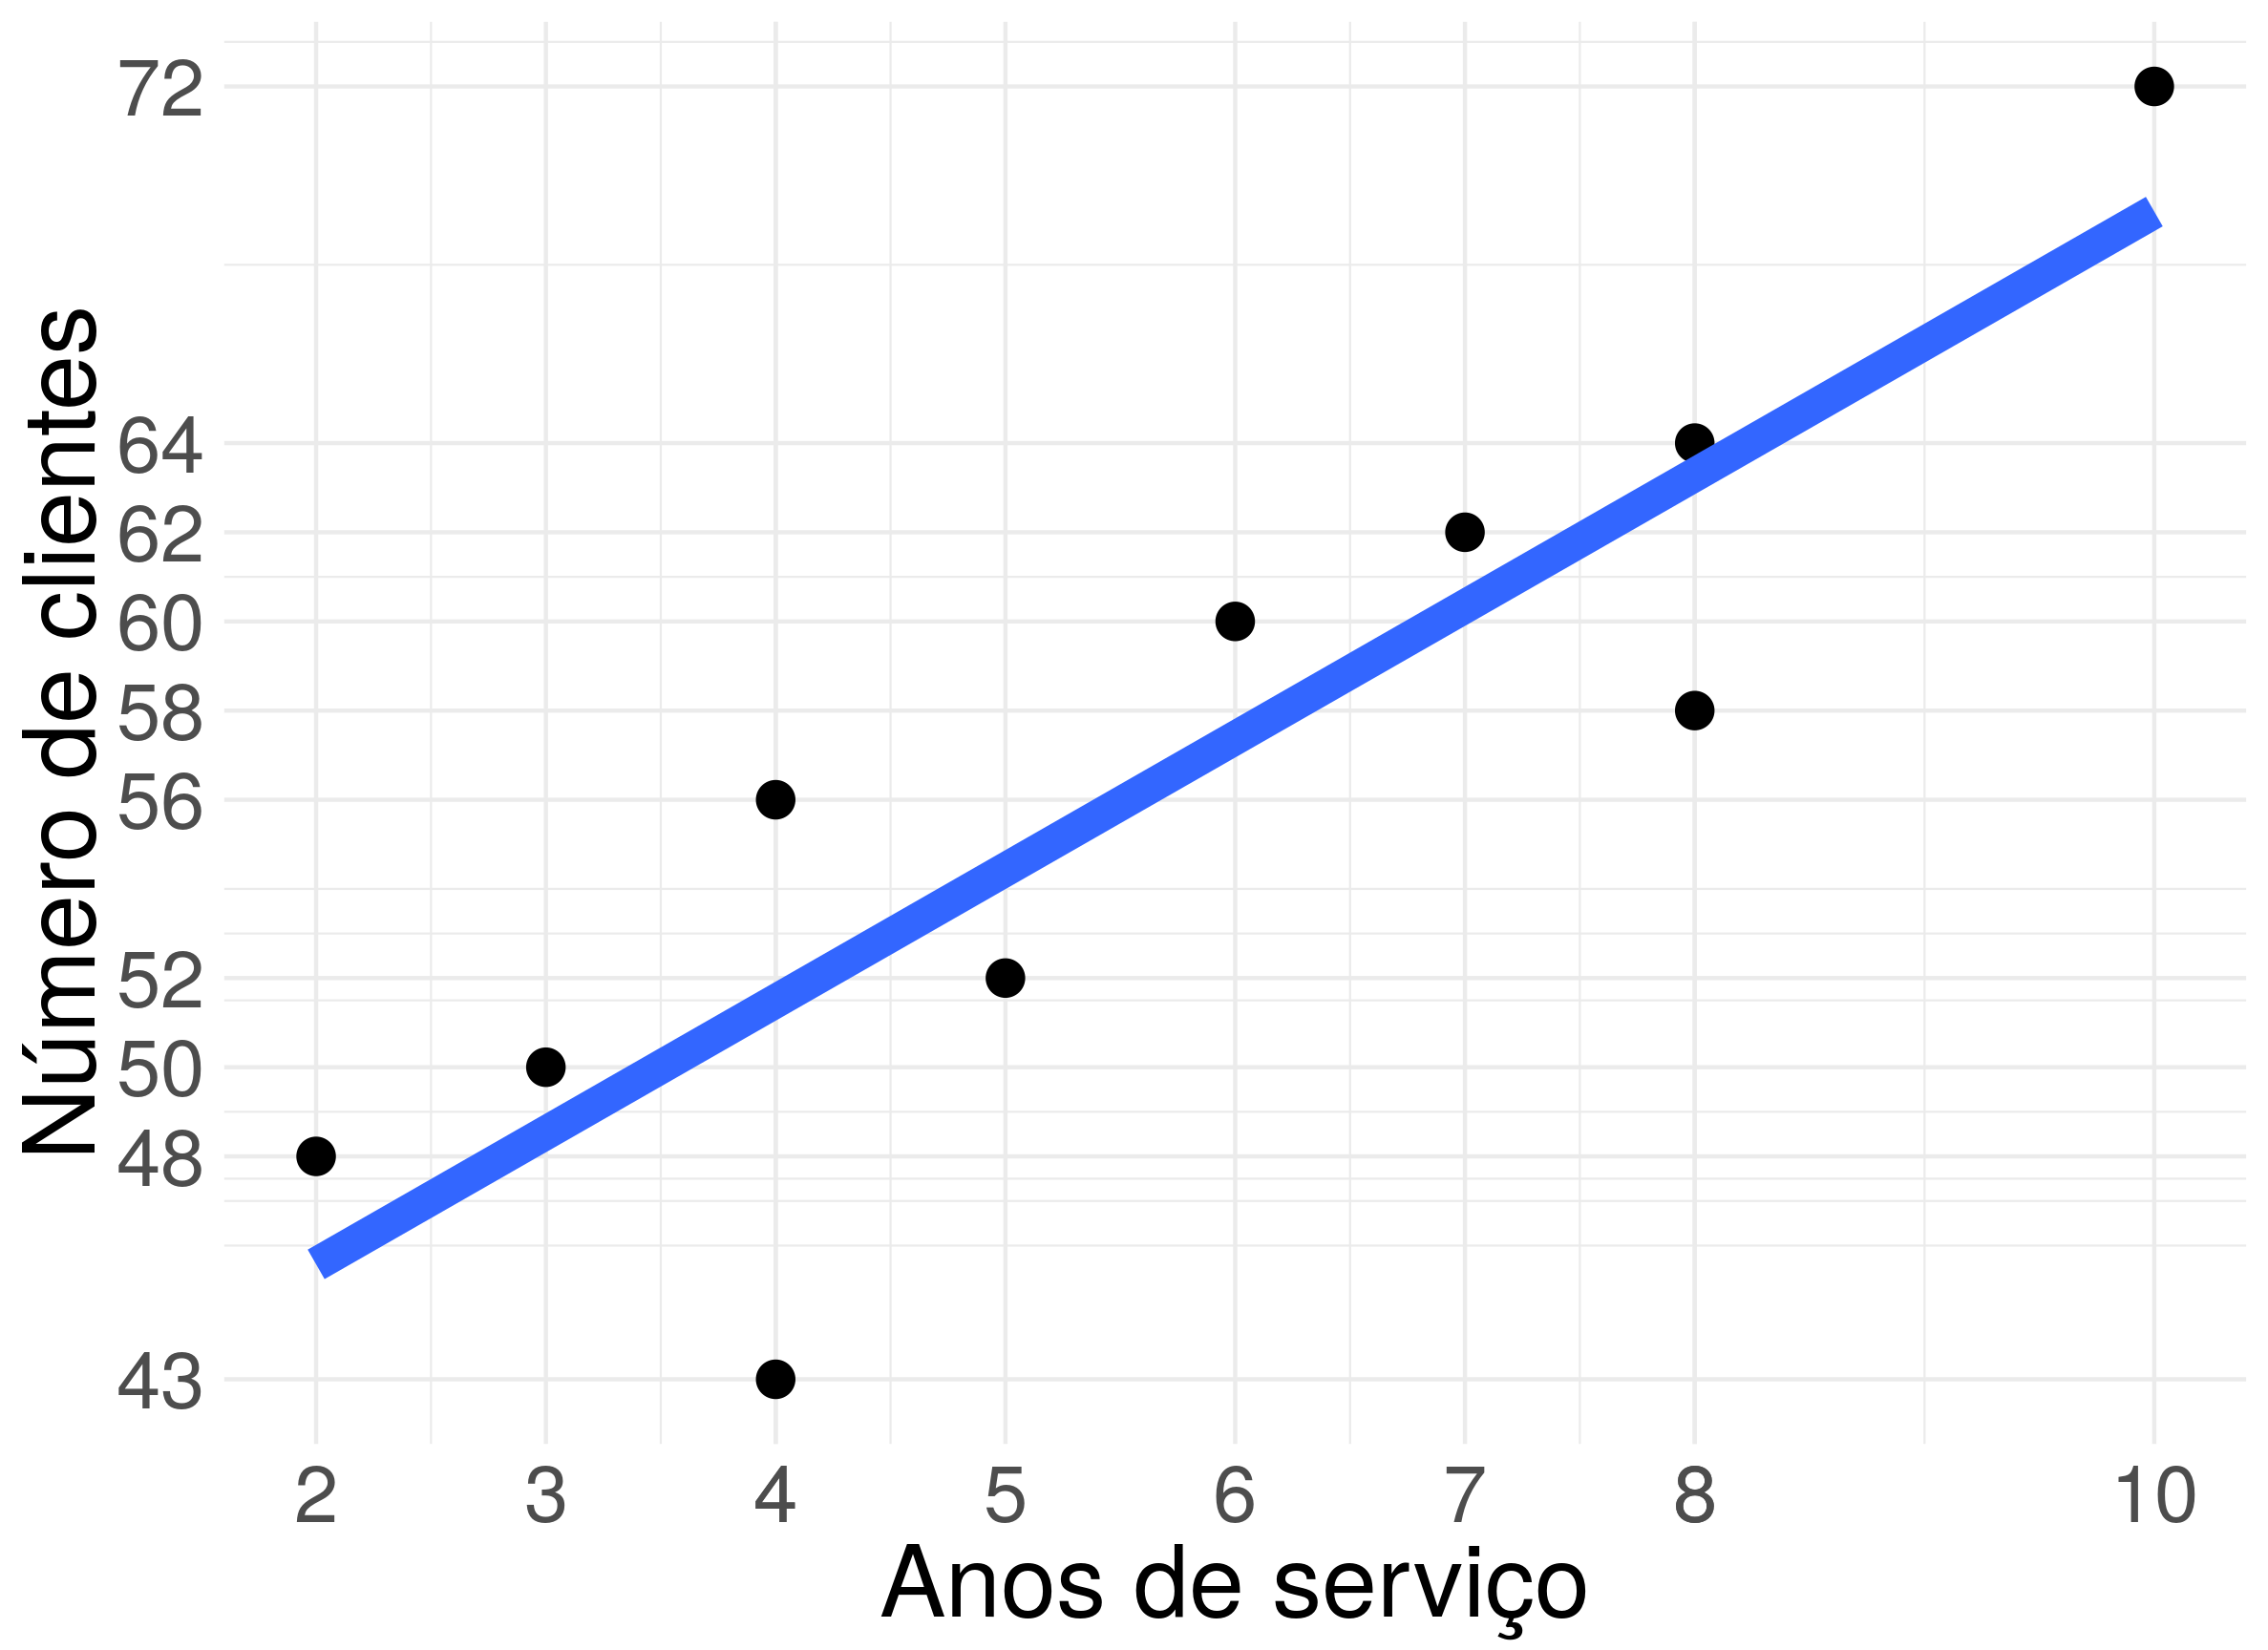
\includegraphics[width = 0.7\linewidth]{figures/positiva.png}
		\caption{Gráfico de dispersão: associação positiva}
		\label{fig:associacao-positiva}
	\end{figure}	
\end{block}

\end{frame}

\begin{frame}{Associação entre variáveis quantitativas}

\begin{block}{Exemplo}
	Numa pesquisa feita com 10 famílias com renda bruta mensal entre 10 e 60 salários mínimos, mediram-se:
	\begin{description}
		\item[$X$] renda bruta mensal (expressa em número de salários mínimos);
		\item[$Y$]  a porcentagem da renda bruta anual gasta com assistência médica.
	\end{description}
	Os dados estão na Tabela~\ref{tab:negativa}.
	
	\begin{table}[ht]
		\centering
		\scalebox{0.6}{
		\begin{tabular}{l|c|c}
			\toprule[0.05cm]
			Família & X & Y \\ 
			\midrule[0.025cm]
			A & 12 & 7,2 \\ 
			B & 16 & 7,4 \\ 
			C & 18 & 7,0 \\ 
			D & 20 & 6,5 \\ 
			E & 28 & 6,6 \\ 
			F & 30 & 6,7 \\ 
			G & 40 & 6,0 \\ 
			H & 48 & 5,6 \\ 
			I & 50 & 6,0 \\ 
			J & 54 & 5,5 \\ 
			\bottomrule[0.05cm]
		\end{tabular}
		}
		\caption{Renda bruta mensal (X) e porcentagem da renda gasta em saúde (Y) para 10 famílias.} 
		\label{tab:negativa}
	\end{table}
		
\end{block}
\end{frame}

\begin{frame}{Associação entre variáveis quantitativas}

\begin{block}{Solução}
	\begin{figure}[htbp]
		\centering
		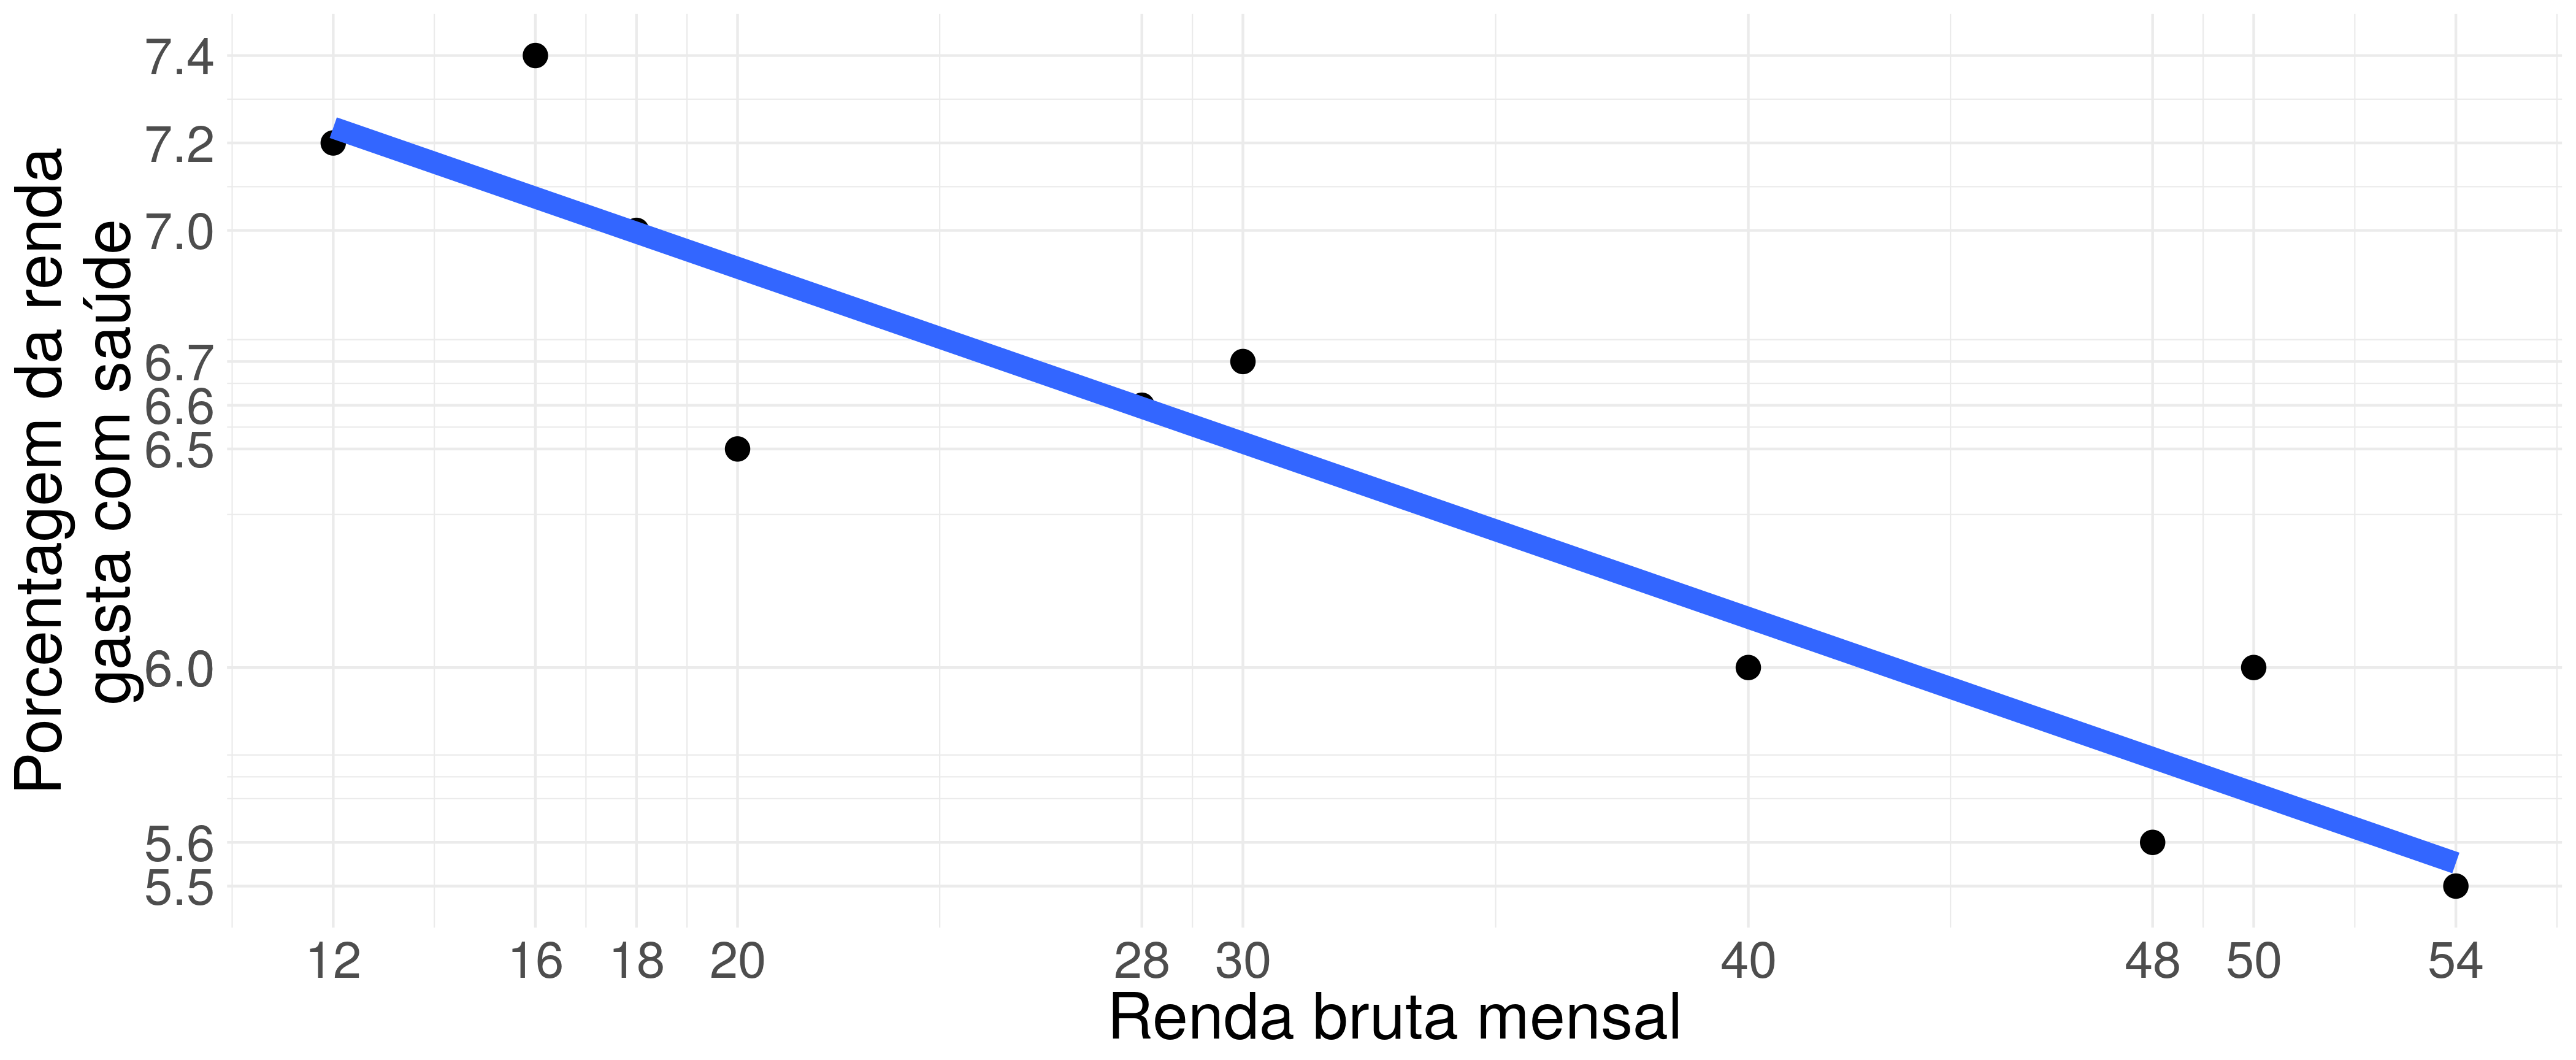
\includegraphics[width = 1.05\linewidth]{figures/negativa.png}
		\caption{Gráfico de dispersão: associação negativa}
		\label{tab:associacao-negativa}
	\end{figure}	
\end{block}

\end{frame}

\begin{frame}{Associação entre variáveis quantitativas}

\begin{block}{Exemplo}
	Oito indivíduos foram submetidos a um teste sobre conhecimento de língua estrangeira e, em seguida, mediu-se o tmepo gasto para cada um aprender a operar uma determinada máquina. As variáveis medidas foram:
	\begin{description}
		\item[$X$] resultado obtido no teste (máximo = 100 pontos);
		\item[$Y$] tempo, em minutos, necessário para operar a máquina satisfatoriamente.
	\end{description}
	Os dados estão na Tabela~\ref{tab:nula}.
	\begin{table}[ht]
		\centering
		\scalebox{0.65}{
		\begin{tabular}{l|cc}
			\toprule[0.05cm]
			Indivíduo & X & Y \\ 
			\midrule[0.025cm]
			A & 45 & 343 \\ 
			B & 52 & 368 \\ 
			C & 61 & 355 \\ 
			D & 70 & 334 \\ 
			E & 74 & 337 \\ 
			F & 76 & 381 \\ 
			G & 80 & 345 \\ 
			H & 90 & 375 \\ 
			\bottomrule[0.05cm]
		\end{tabular}
		}
		\caption{Amostra de famílias.} 
		\label{tab:nula}
	\end{table}	
\end{block}

\end{frame}

\begin{frame}{Associação entre variáveis quantitativas}

\begin{block}{Solução}
	\begin{figure}[htbp]
		\centering
		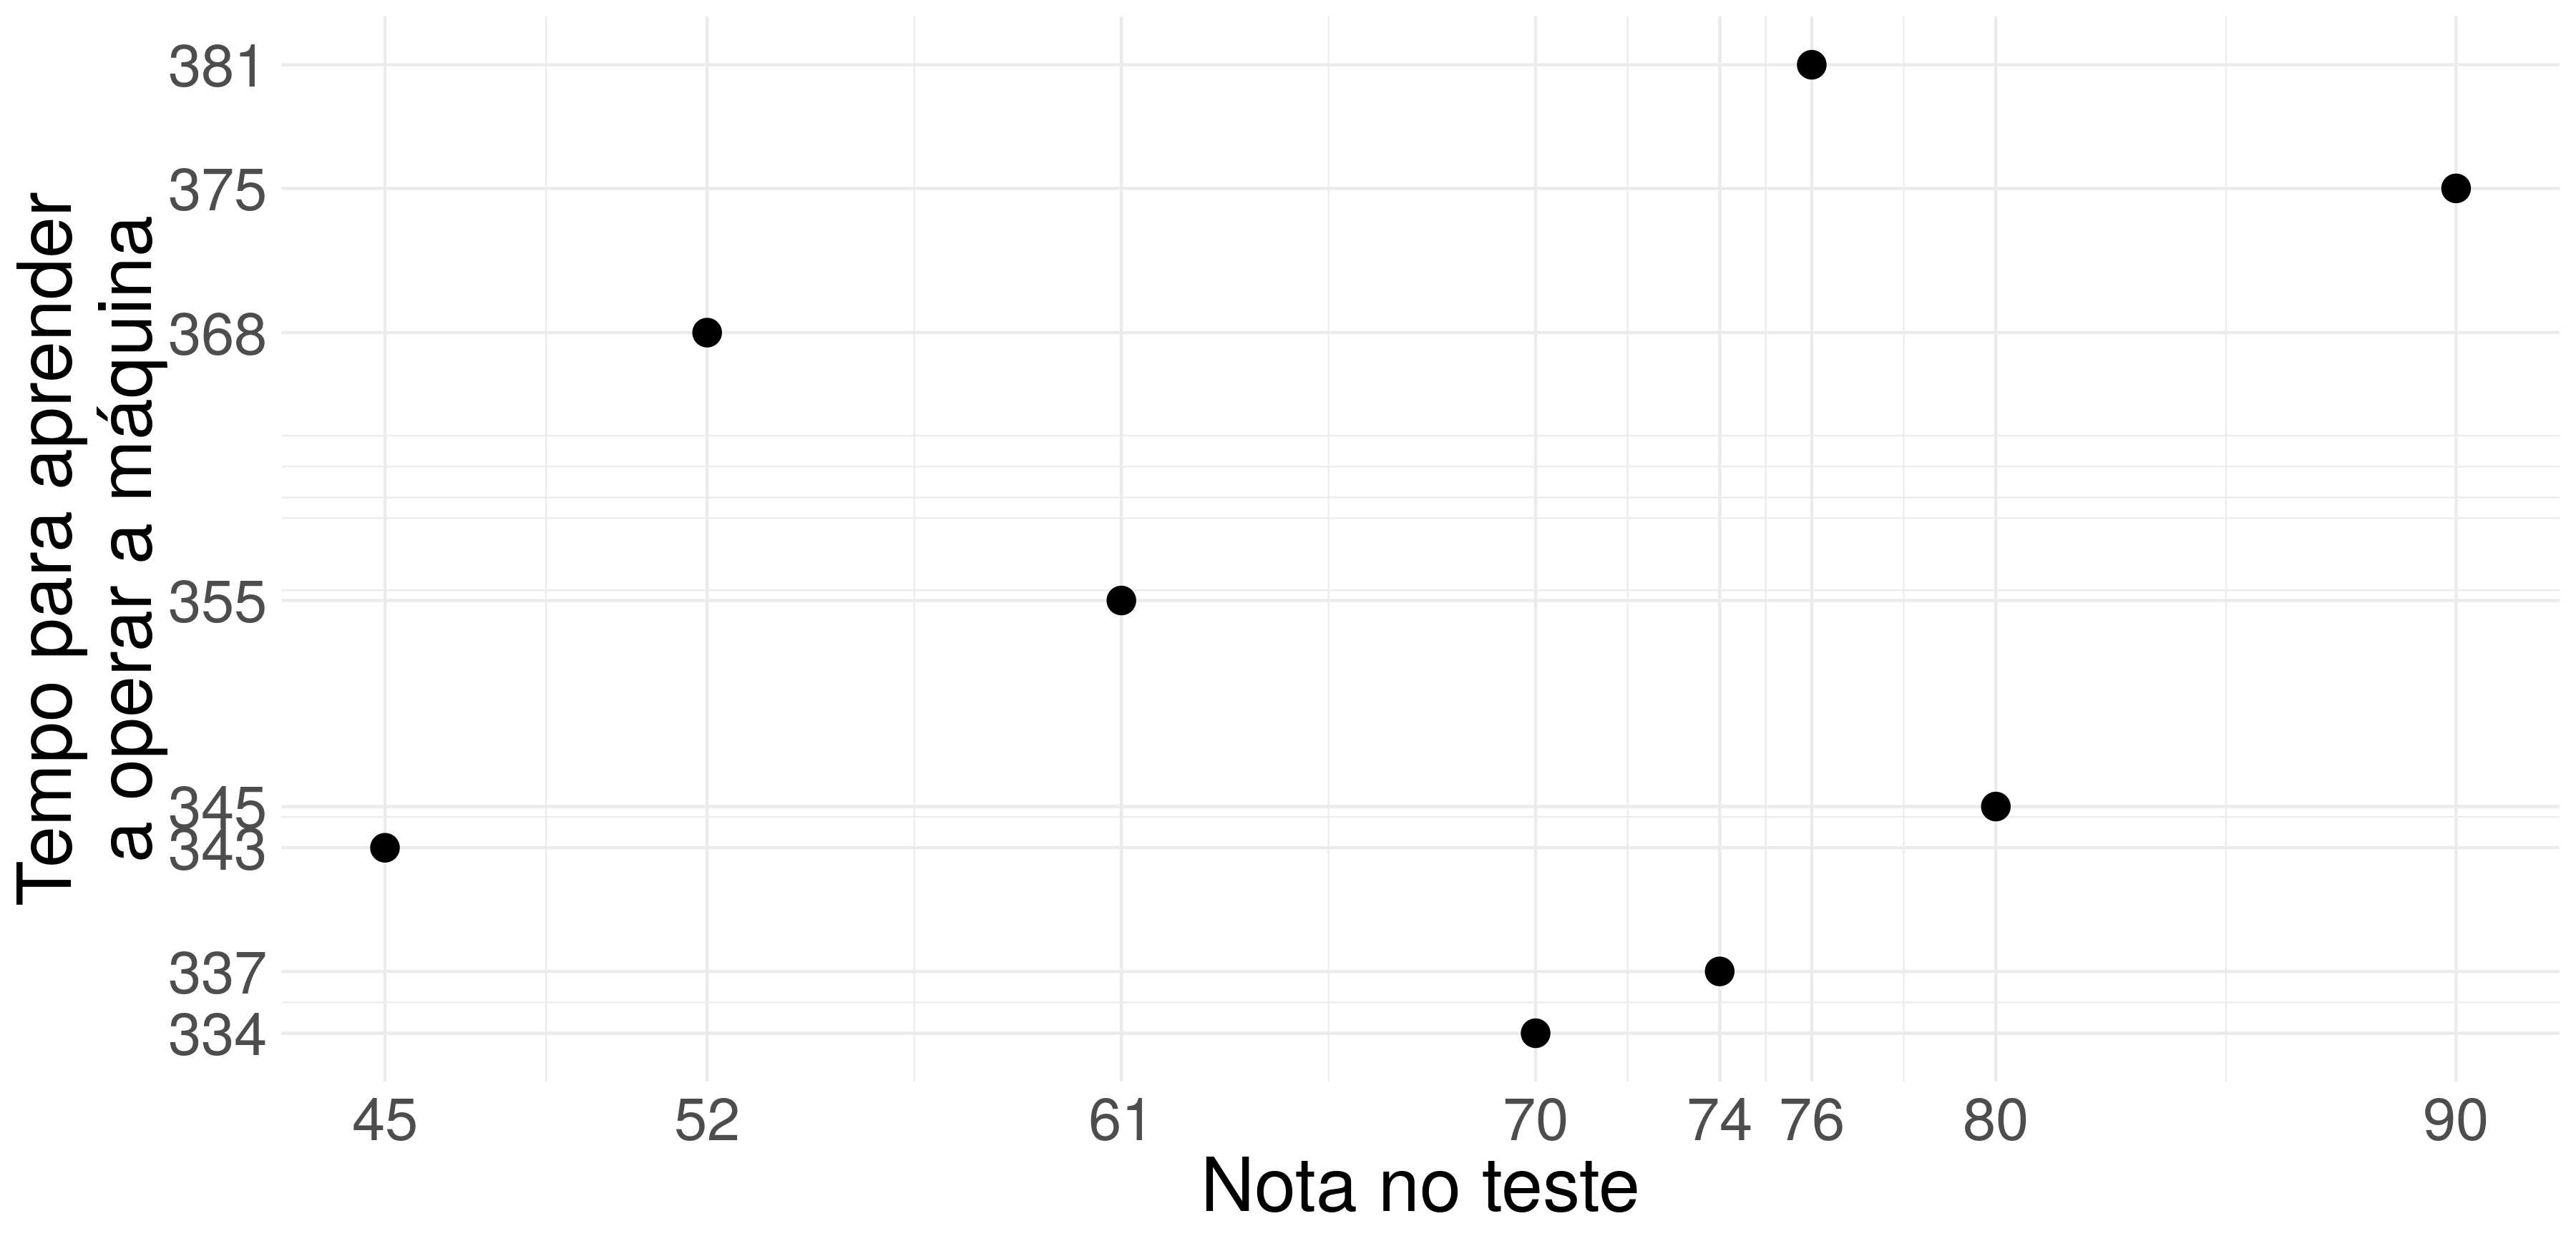
\includegraphics[width = \linewidth]{figures/nula.png}
		\caption{Gráfico de dispersão: associação nula}
		\label{tab:associacao-nula}
	\end{figure}		
\end{block}

\end{frame}


\subsection{Coeficiente de correlação linear de Pearson}

\begin{frame}{Coeficiente de correlação de Pearson}

\footnotesize
	Podemos resumir a associação entre duas variáveis quantitativas em três casos (para variáveis padronizadas -- subtrair a média e dividir pelo desvio padrão):
	
	
	\begin{minipage}[b]{0.24\linewidth}
		\begin{figure}[htbp]
			\centering
			\caption{\footnotesize  Associação positiva.}
			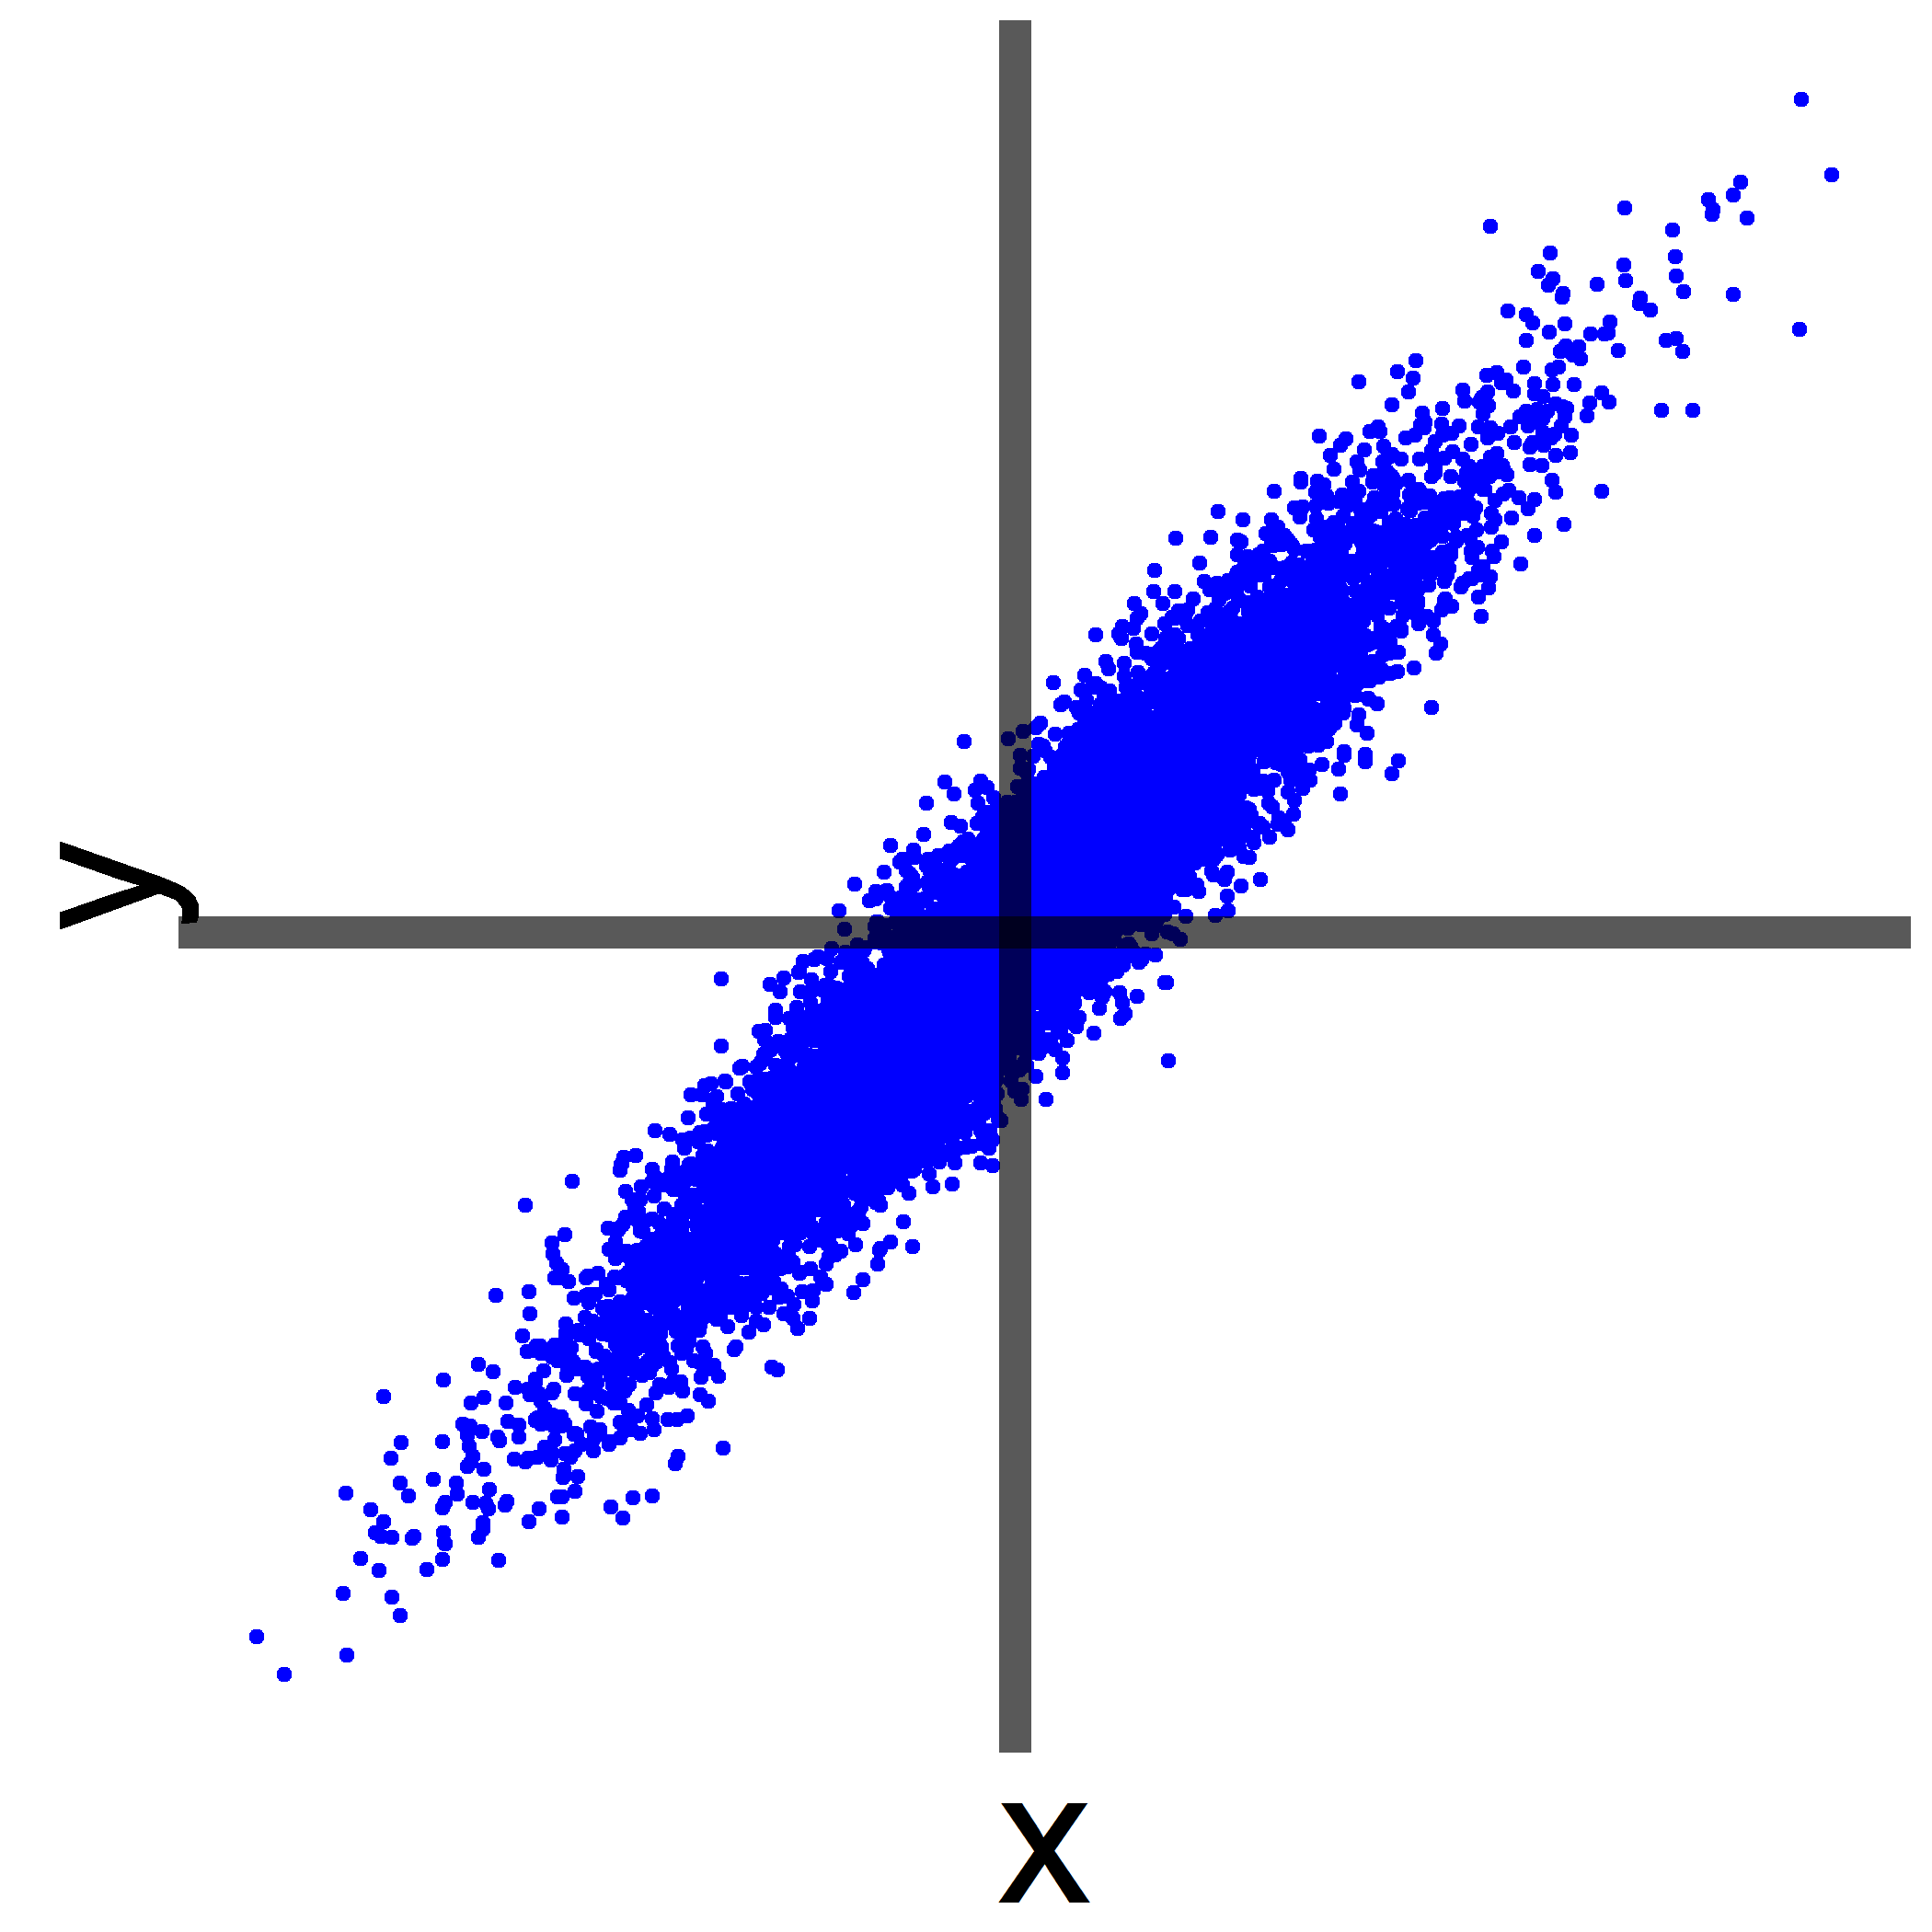
\includegraphics[width= 1.5cm]{figures/a_positiva.png}
		\end{figure}
	\end{minipage}%
	\begin{minipage}[b]{0.24\linewidth}
		\begin{center}
				A maioria dos pontos estão no primeiro e no terceiro quadrantes e a maioria das multiplicações das coordenadas destes pontos são positivas.
		\end{center}
	\end{minipage}	
	\begin{minipage}[b]{0.24\linewidth}
		\begin{figure}[htbp]
			\centering
			\caption{\footnotesize  Associação negativa.}
			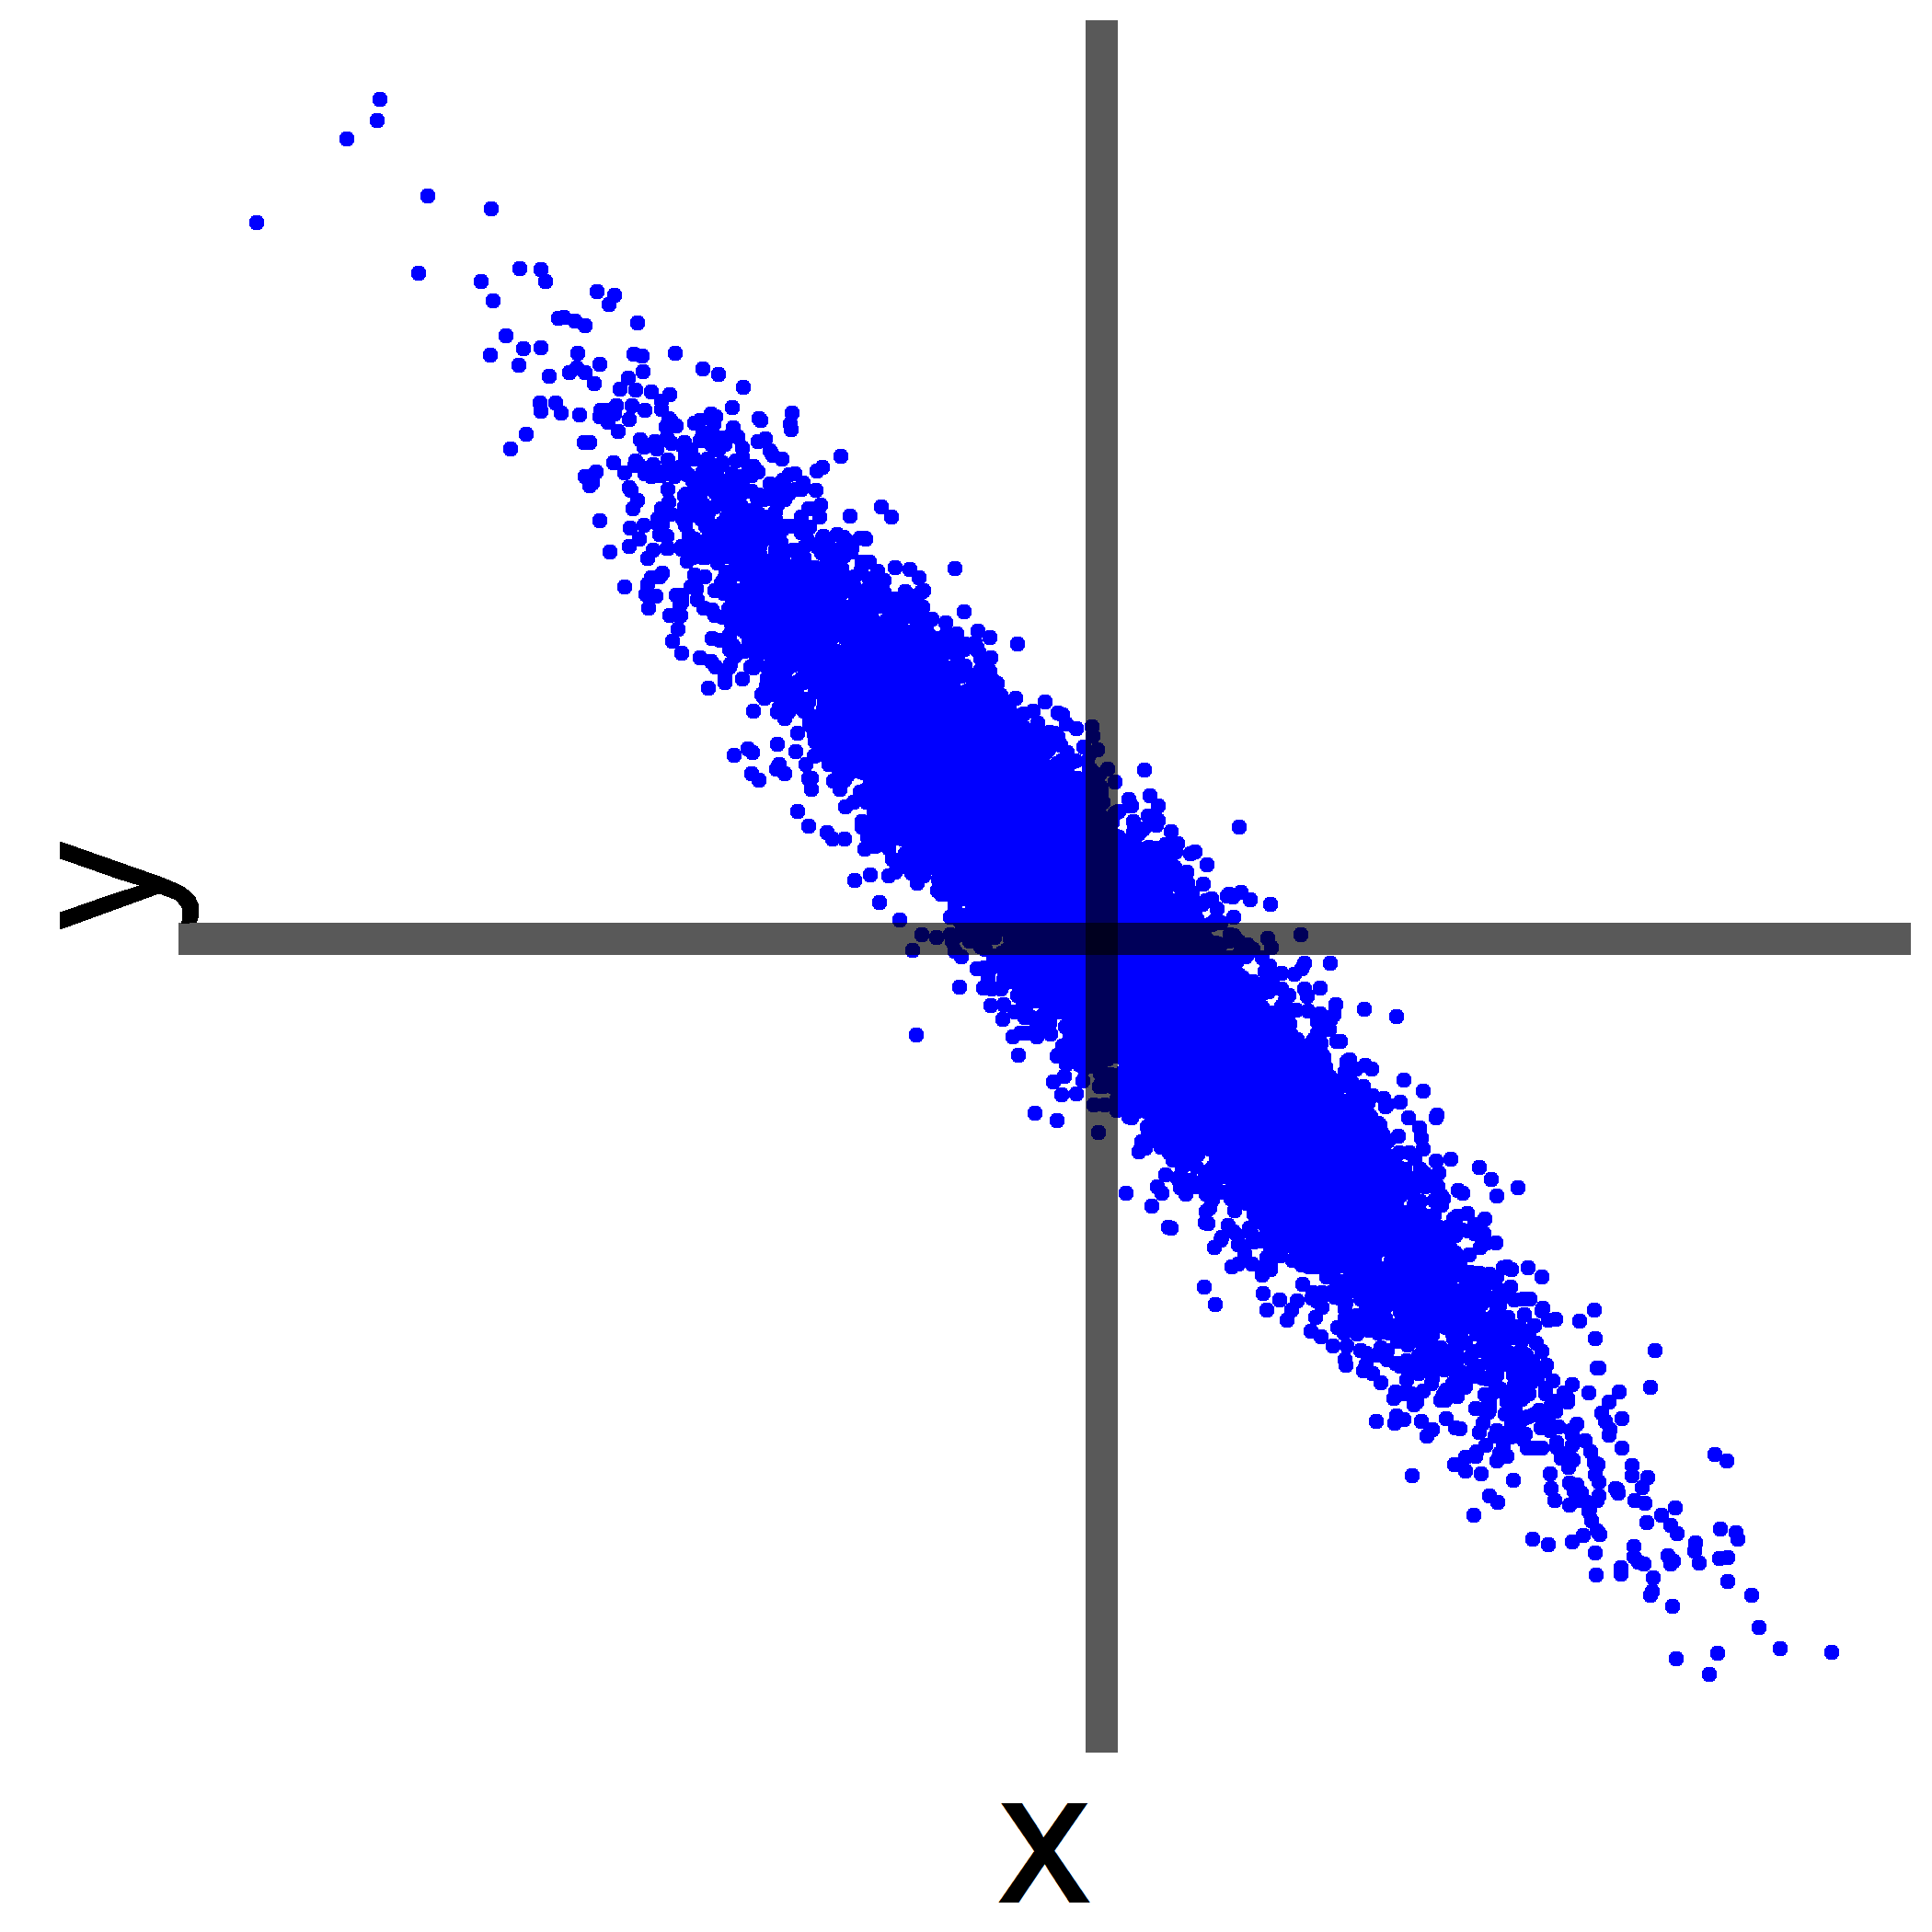
\includegraphics[width= 1.5cm]{figures/a_negativa.png}
		\end{figure}
	\end{minipage}%
	\begin{minipage}[b]{0.24\linewidth}
		\begin{center}
				A maioria dos pontos estão no segundo e quarto quadrantes e a maioria das multiplicações das coordenadas destes pontos são negativas.
		\end{center}
	\end{minipage} \\
	\begin{center}
		\begin{minipage}[b]{0.35\linewidth}
			\begin{figure}[htbp]
				\centering
				\caption{\footnotesize Associação nula.}
				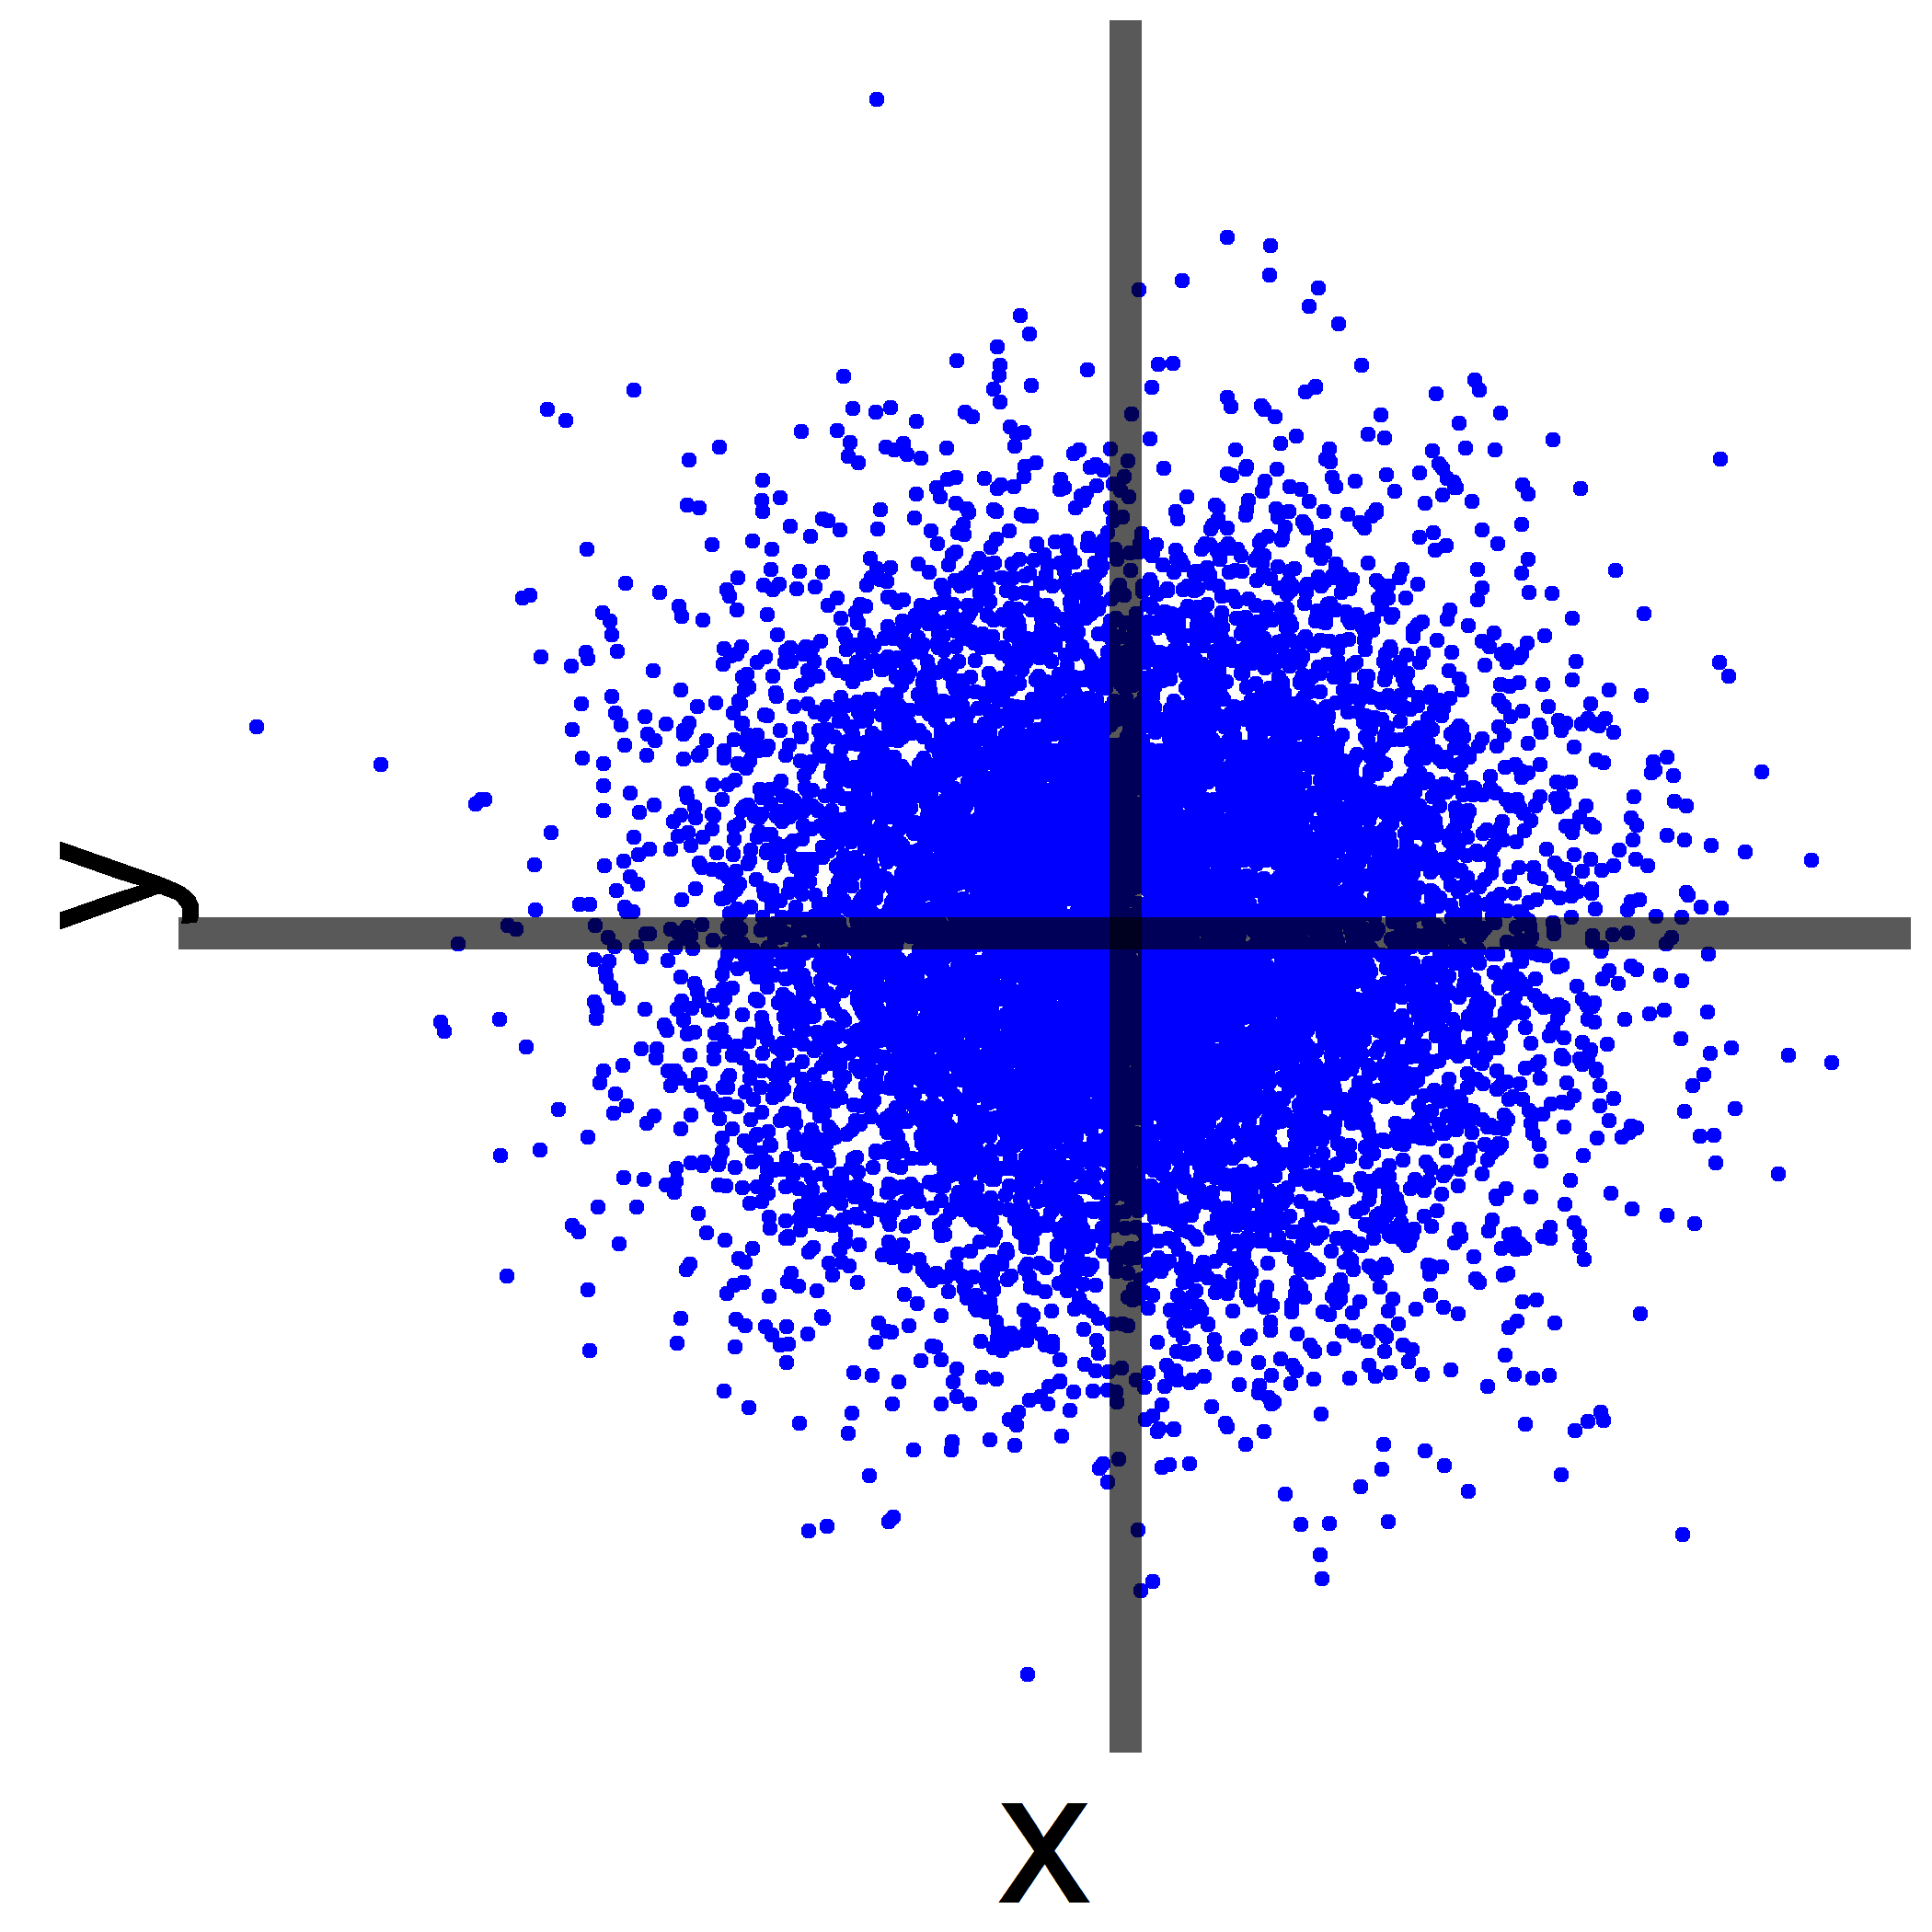
\includegraphics[width= 1.5cm]{figures/a_nula.png}
			\end{figure}
		\end{minipage}%
		\begin{minipage}[b]{0.35\linewidth}
			\begin{center}
					Uma igual proporção de pontos estão no primeiro, no segundo e no terceiro quadrantes.
			\end{center}
		\end{minipage} 
	\end{center}
	
\normalsize
\end{frame}

\begin{frame}{Coeficiente de correlação linear de Pearson}

\small
\begin{block}{Motivação}
	Consideramos as variáveis padronizadas $z_i = \frac{x_i - \bar{x}}{dp(X)}, i=1, \dots, n$ e $w_i = \frac{y_i - \bar{y}}{dp(Y)}$ e multiplicamos as coordenadas $z_i \cdot w_i, i=1, \dots, n$. Se:
	\begin{itemize}
		\item A maioria dos valores  $z_i \cdot w_i, i=1, \dots, n$ são positivos, então a associação é positiva. Ou seja, se a média dos valores $z_i \cdot w_i, i=1, \dots, n$ é positiva, a associação é positiva.
		\item A maioria dos valores  $z_i \cdot w_i, i=1, \dots, n$ são negativos, então a associação é negativa. Ou seja, se a média dos valores $z_i \cdot w_i, i=1, \dots, n$ é negativa, a associação é negativa.
		\item Se aproximadamente $50\%$ dos valores $z_i \cdot w_i, i=1, \dots, n$ são negativos e $50\%$ dos valores são positivos, então a associação é nula. Ou seja,  se a média dos valores $z_i \cdot w_i, i=1, \dots, n$ é aproximadamente zero, então a associação é nula.
	\end{itemize}
\end{block}
\vfill

\begin{block}{Definição}
	Definimos o Coeficiente de Correlação Linear de Pearson por
	\begin{align*}
	r =	Corr(X, Y) = \dfrac{ \frac{x_1 - \bar{X}}{dp(X)} \cdot \frac{y_1 - \bar{Y}}{dp(Y)} + \frac{x_2 - \bar{X}}{dp(X)} \cdot \frac{y_2 - \bar{Y}}{dp(Y)} + \cdots + \frac{x_n - \bar{X}}{dp(X)} \cdot \frac{y_n - \bar{Y}}{dp(Y)} }{n}.
	\end{align*}
\end{block}
\normalsize

\end{frame}

\begin{frame}{Coeficiente de correlação linear de Pearson}

\footnotesize
\begin{block}{Propriedades}
	\begin{itemize}
		\item $r = Corr(X, Y) \in [-1,1]$;
		\item $r=Corr(X, Y) \approx 0$ se, e somente se, $X$ e $Y$ não estão associadas;
		\item $r=Corr(X, Y) > 0$ se, e somente se, $X$ e $Y$ estão positivamente associadas;
		\item $r=Corr(X, Y) < 0$ se, e somente se, $X$ e $Y$  estão negativamente associadas;
		\item 
		$
		r = Corr(X, Y) = \dfrac{S_{xy} - n \bar{x}\bar{y} }{ \sqrt{(S_{x^2}- n \bar{x}^2)(S_{y^2} - n\bar{y}^2)} }
		$ em que 
		\begin{itemize}
			\item $S_{xy} = x_1 y_1 + x_2 y_2 + \dots + x_n y_n$;
			\item $S_{x^2} = x_1^2 + x_2^2 + \dots + x_n^2$;
			\item $S_{y^2} = y_1^2 + y_2^2 + \dots + y_n^2$.
		\end{itemize}
	\end{itemize}
\end{block}
\vfill

\begin{block}{Regra de ouro}
		\begin{table}[htbp]
			\centering
			\scalebox{0.75}{
			\begin{tabular}{lc|c|lc}
				\toprule[0.05cm]
				$Corr(X, Y)$ & Tipo de Associação & & $Corr(X, Y)$ & Tipo de Associação \\
				\midrule[0.05cm]
				$(0,8;1]$ & Forte associação positiva & & $[-1;-0,8)$ & Forte associação negativa\\
				$(0,2;0,8]$ & Associação moderada positiva  & & $[-0,8;-0,2)$ & Associação moderada negativa\\
				$[0;0,2]$ & Associação nula & & $[-0,2;0]$ & Associação nula\\
				\bottomrule[0.05cm]
			\end{tabular}
			}
		\end{table}
\end{block}
\normalsize

\end{frame}

\begin{frame}{Coeficiente de correlação de Pearson}

\begin{block}{Exemplo}
	Considere as variáveis  $X$: anos de serviço e $Y$: número de clientes da Tabela~\ref{tab:corr}. Calcule o coeficiente de correlação.
\end{block}


\begin{block}{Solução}
	Note que $\bar{x}= 5,7$, $\bar{y}=56,5$, $dp(X)=2,41$ e $dp(Y)=8,11$.
	\begin{table}[ht]
		\centering
		
		\scalebox{0.55}{
		\begin{tabular}{l|cc|cc|c}
			\toprule[0.05cm]
			Agente & $X$ & $Y$ & $Z=\frac{X - \bar{X}}{dp(X)}$ & $W = \frac{Y - \bar{Y}}{dp(Y)}$ & $Z \cdot W$ \\ 
			\midrule[0.05cm]
			A & 2 & 48 & -1,54 & -1,05 & 1,61 \\ 
			B & 3 & 50 & -1,12 & -0,80 & 0,90 \\ 
			C & 4 & 56 & -0,71 & -0,06 & 0,04 \\ 
			D & 5 & 52 & -0,29 & -0,55 & 0,16 \\ 
			E & 4 & 43 & -0,71 & -1,66 & 1,17 \\ 
			F & 6 & 60 & 0,12 & 0,43 & 0,05 \\ 
			G & 7 & 62 & 0,54 & 0,68 & 0,37 \\ 
			H & 8 & 58 & 0,95 & 0,18 & 0,18 \\ 
			I & 8 & 64 & 0,95 & 0,92 & 0,88 \\ 
			J & 10 & 72 & 1,78 & 1,91 & 3,41 \\ 
			\midrule[0.05cm]
			Total & 57 & 565 & 0 & 0 & 8,77\\
			\bottomrule[0.05cm]
		\end{tabular}
		}
		\caption{Cálculo do coeficiente de correlação linear de Pearson.} 
		\label{tab:corr}
	\end{table}
	Então  $r = \dfrac{8,77}{10} = 0,88$ e as variáveis $X$ e $Y$ estão positivamente e fortemente associadas.
\end{block}
\end{frame}

\begin{frame}{Coeficiente de correlação linear de Pearson}

\begin{block}{Exemplo}
	Está sendo estudado o efeito do teor de ferro na capacidade de vigas de concreto. Os da Tabela~\ref{tab:vigas} apresentam os resultados obtidas em uma amostra. Desenhe o gráfico de dispersão e calcule o coeficiente de correlação entre as duas variáveis.
	\begin{table}[ht]
		\centering
		\scalebox{0.8}{
		\begin{tabular}{l|cccccccccc}
			\toprule[0.05cm]
			X: ferro(\% peso) & 5,4 & 6,8 & 6,9 & 7,3 & 7,7 & 8,1 & 8,2 & 8,5 & 8,6 & 8,9 \\ \midrule[0.025cm]
			Y: Carga (ton. / m$^2$) & 2,1 & 2,2 & 2,9 & 2,9 & 3,0 & 3,1 & 3,1 & 3,1 & 3,4 & 3,5 \\ \bottomrule[0.05cm]
		\end{tabular}
		}
		\caption{Amostra com 10 vigas.} 
		\label{tab:vigas}
	\end{table}
	Note que $S_{x}= 76,4$, $S_{Y}=29,3$, $S_{x^2}=593,86$, $S_{y^2}=87,71$ e $S_{xy} = 227,85$.
\end{block}
\end{frame}

\begin{frame}{Coeficiente de correlação linear de Pearson}

\begin{block}{Solução}
	\begin{minipage}{0.4\linewidth}
		\begin{figure}[htbp]
			\centering
			\caption{Gráfico de dispersão entre $X$ e $Y$.}
			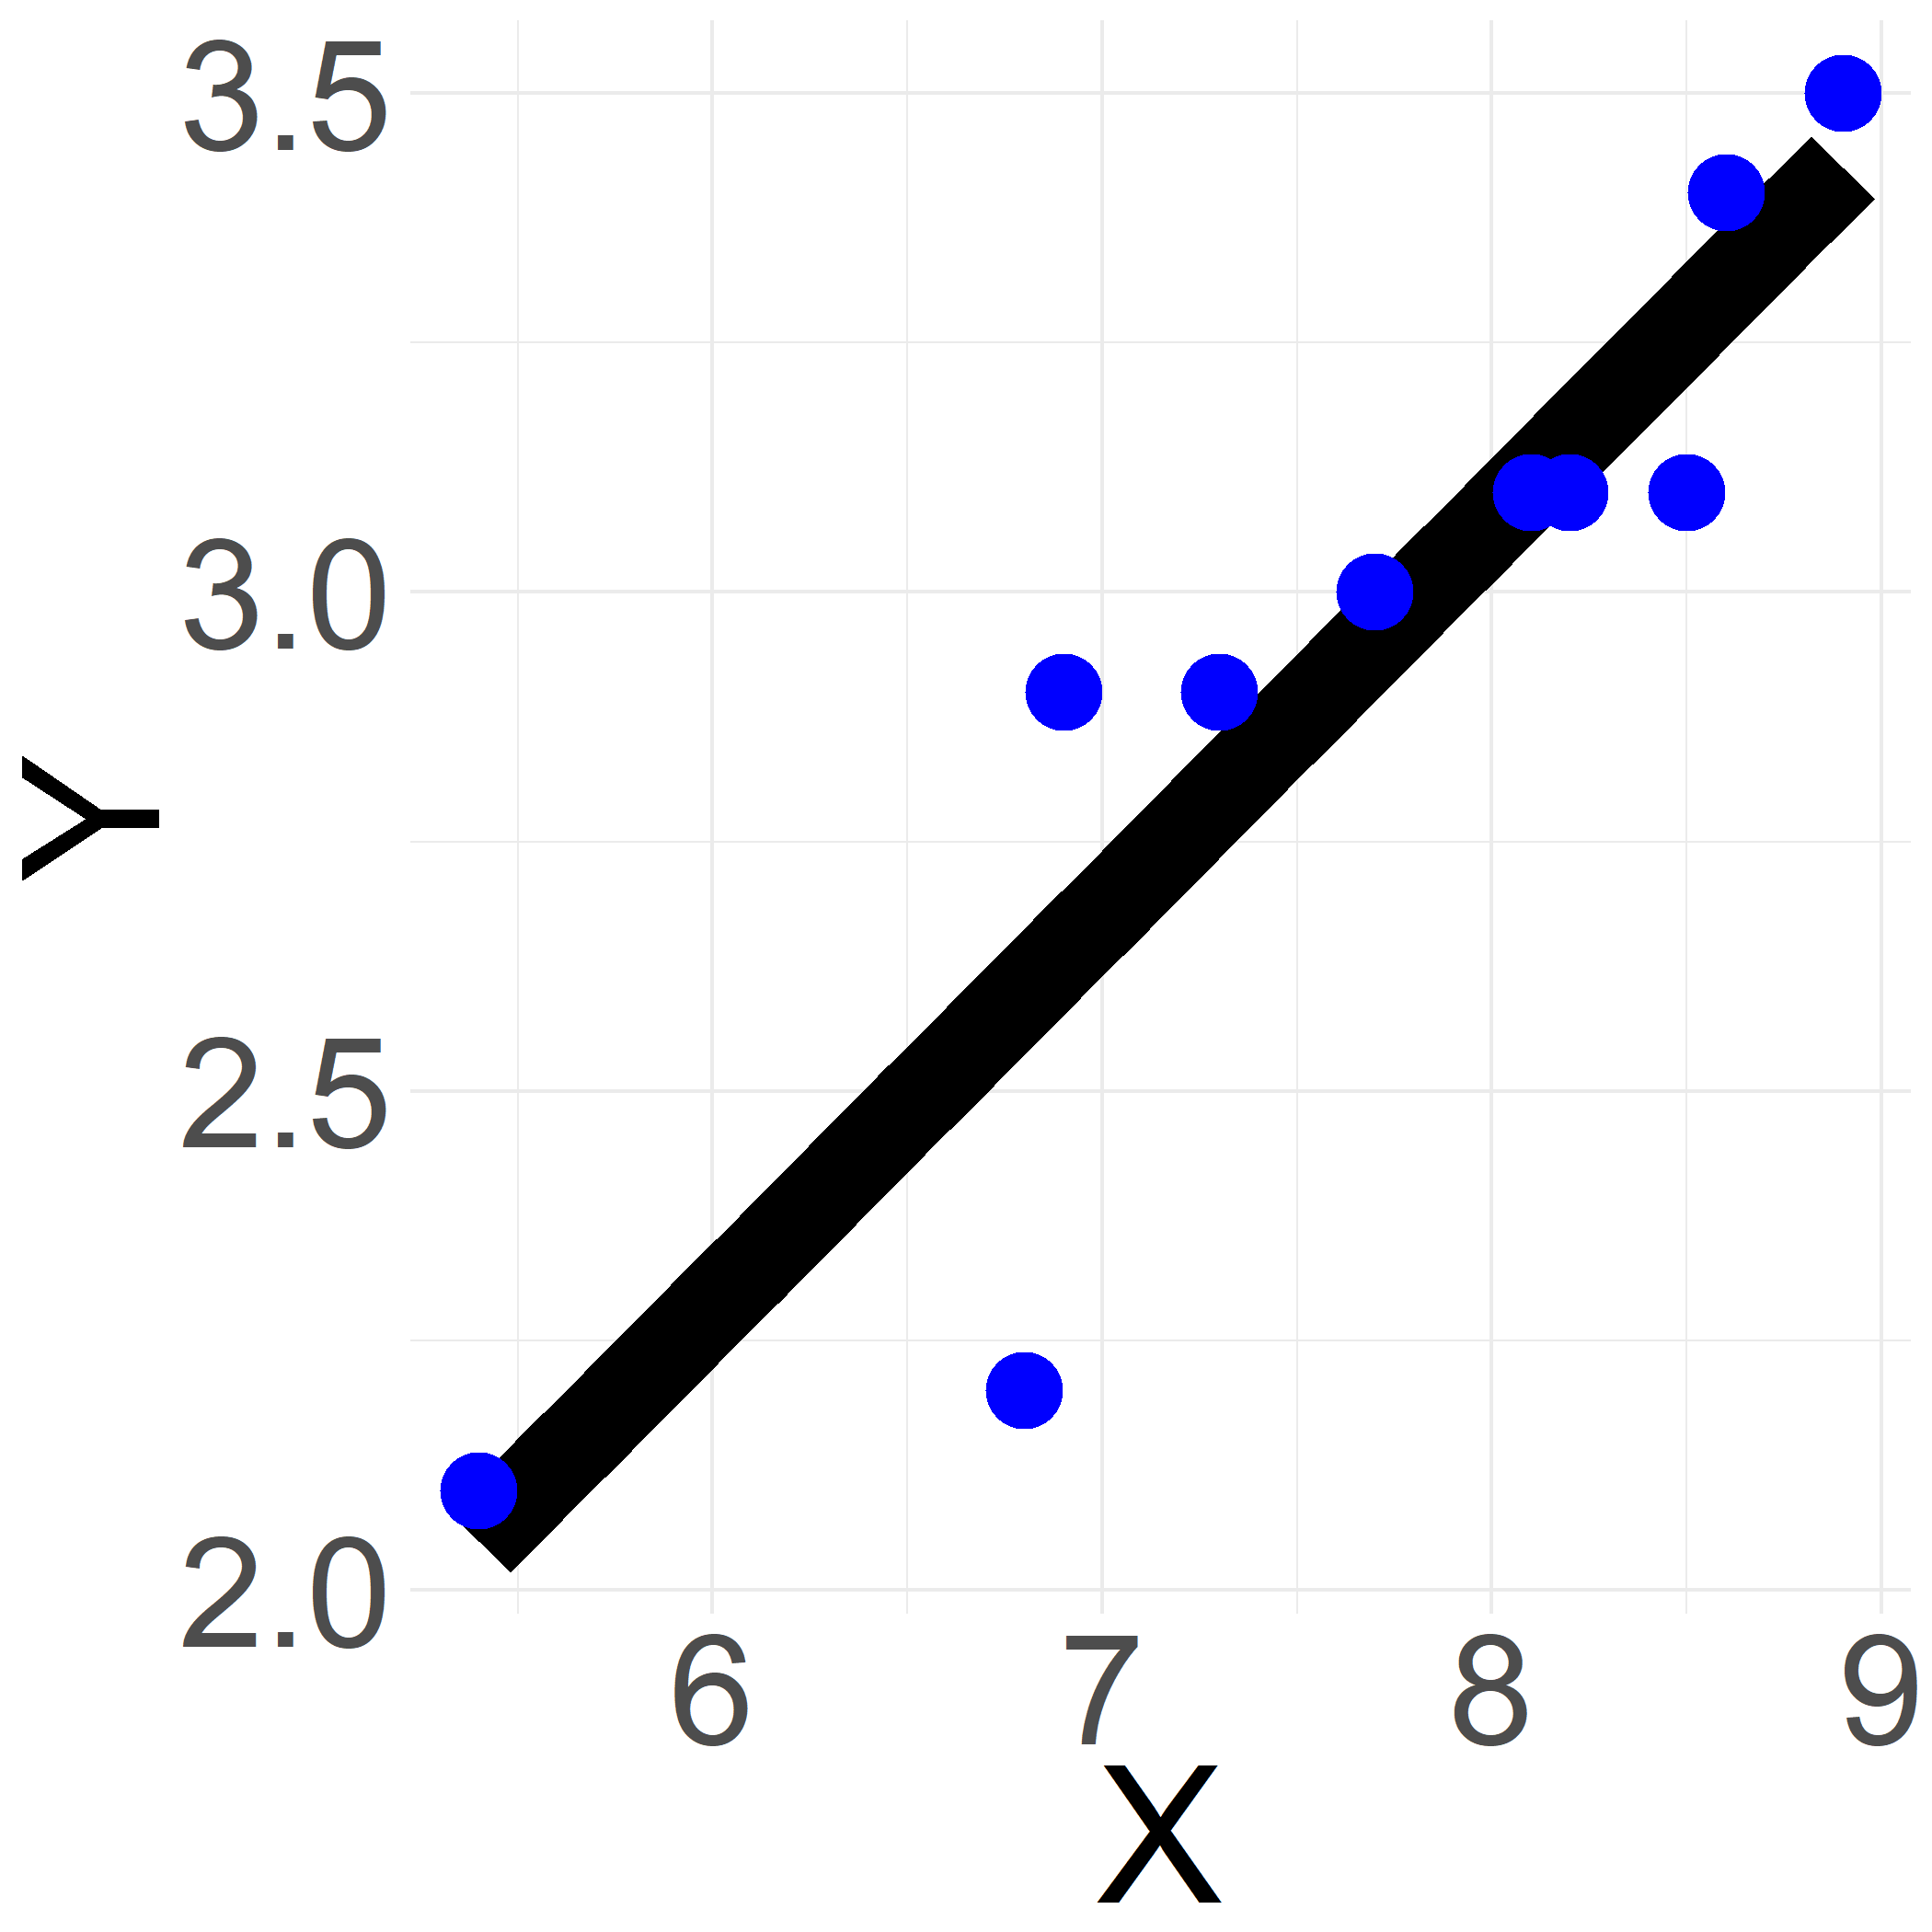
\includegraphics[width=0.75\linewidth]{figures/exemplo2.png}
		\end{figure}
	\end{minipage}
	\begin{minipage}{0.4\linewidth}
		{\small
		\begin{flushleft}
			Note que $\bar{x} = \dfrac{S_x}{n}=\frac{76,4}{10}= 7,64$ e $\bar{y}=\frac{S_y}{n} = \frac{29,3}{10} = 2,93$, então
			\begin{align*}
			r &= \dfrac{S_{xy} - n \bar{x} \bar{y}}{\sqrt{(S_{x^2} - n \bar{x})(S_{y^2} - n \bar{y})}}\\
			&= \dfrac{227,85 - 10 \cdot 7,64 \cdot 2,93}{\sqrt{(593,86 - 10 \cdot 7,64^2) (87,71 - 10 \cdot 2,93^2)}}\\
			&= 0,92.
			\end{align*}
		\end{flushleft}
		}
	\end{minipage}

Notamos no gráfico de dispersão que as variáveis $X$ e $Y$ estão positivamente associadas, ou seja, quanto maior  a porcentagem de ferro maior a capacidade da viga. Além disso, o coeficiente de correlação linear de Pearson é $0,92$ e temos uma forte associação positiva entre as variáveis.
	
\end{block}

\end{frame}

\begin{frame}{Teste de hipóteses para $\rho$.}

\small

Sejam
\begin{itemize}
	\item $x_{1,1}, \dots, x_{1, n_1}$ valores amostrados da população 1 $x_1 \sim N(\mu_1, \sigma_1^2)$;
	\item $x_{2,1}, \dots, x_{2, n_2}$ valores amostrados da população 1 $x_2 \sim N(\mu_2, \sigma_2^2)$;
	\item $\frac{1}{2} \ln \left( \frac{1 + r}{1 - r} \right) \sim N \left( \frac{1}{2} \ln \left( \frac{1 + \rho}{1 - \rho}\right); \frac{1}{n-3}  \right)$, em que $\rho$ é o coeficiente de correlação linear de Pearson populacional;
	\item $f(x) = \frac{1}{2} \ln \left( \frac{1 + x}{1 - x} \right)$ é chamada de transformação Z de Fisher;
	\item $\alpha$ é o nível de significância (geralmente $\alpha=5\%$). 
\end{itemize}
\vfill

Queremos testar as seguintes hipóteses:
\begin{itemize}
	\item Teste bilateral: $H_0: \rho = \rho_0$ e $H_1: \rho \neq \rho_0$;
	\item Teste unilateral: $H_0: \rho \leq \rho_0$ e $H_1: \rho > \rho_0$;
	\item Teste unilateral: $H_0: \rho \geq \rho_0$ e $H_1: \rho < \rho_0$.
\end{itemize}
\vfill

\textbf{Ideia:} Primeiro calculamos $Z_0 = \frac{ \frac{1}{2} \ln \left( \frac{1 + r}{1 - r} \right) - \frac{1}{2} \ln \left( \frac{1 + \rho_0}{1 - \rho_0} \right) }{\sqrt{\nicefrac{1}{n-3}}}$. Então, 
\begin{itemize}
	\item Teste bilateral: Rejeitamos $H_0: \rho = \rho_0$ se $\lvert Z_0 \rvert$ for grande;
	\item Teste unilateral: Rejeitamos $H_0: \rho \leq \rho_0$ se $Z_0 $ for grande;
	\item Teste unilateral: Rejeitamos $H_0: \rho \geq \rho_0$ se $Z_0 $ for pequeno.
\end{itemize}

\normalsize
\end{frame}

\begin{frame}{Teste de hipóteses para $\rho$.}
\begin{figure}[htbp]
	\centering
	\subfloat[][Teste bilateral.]{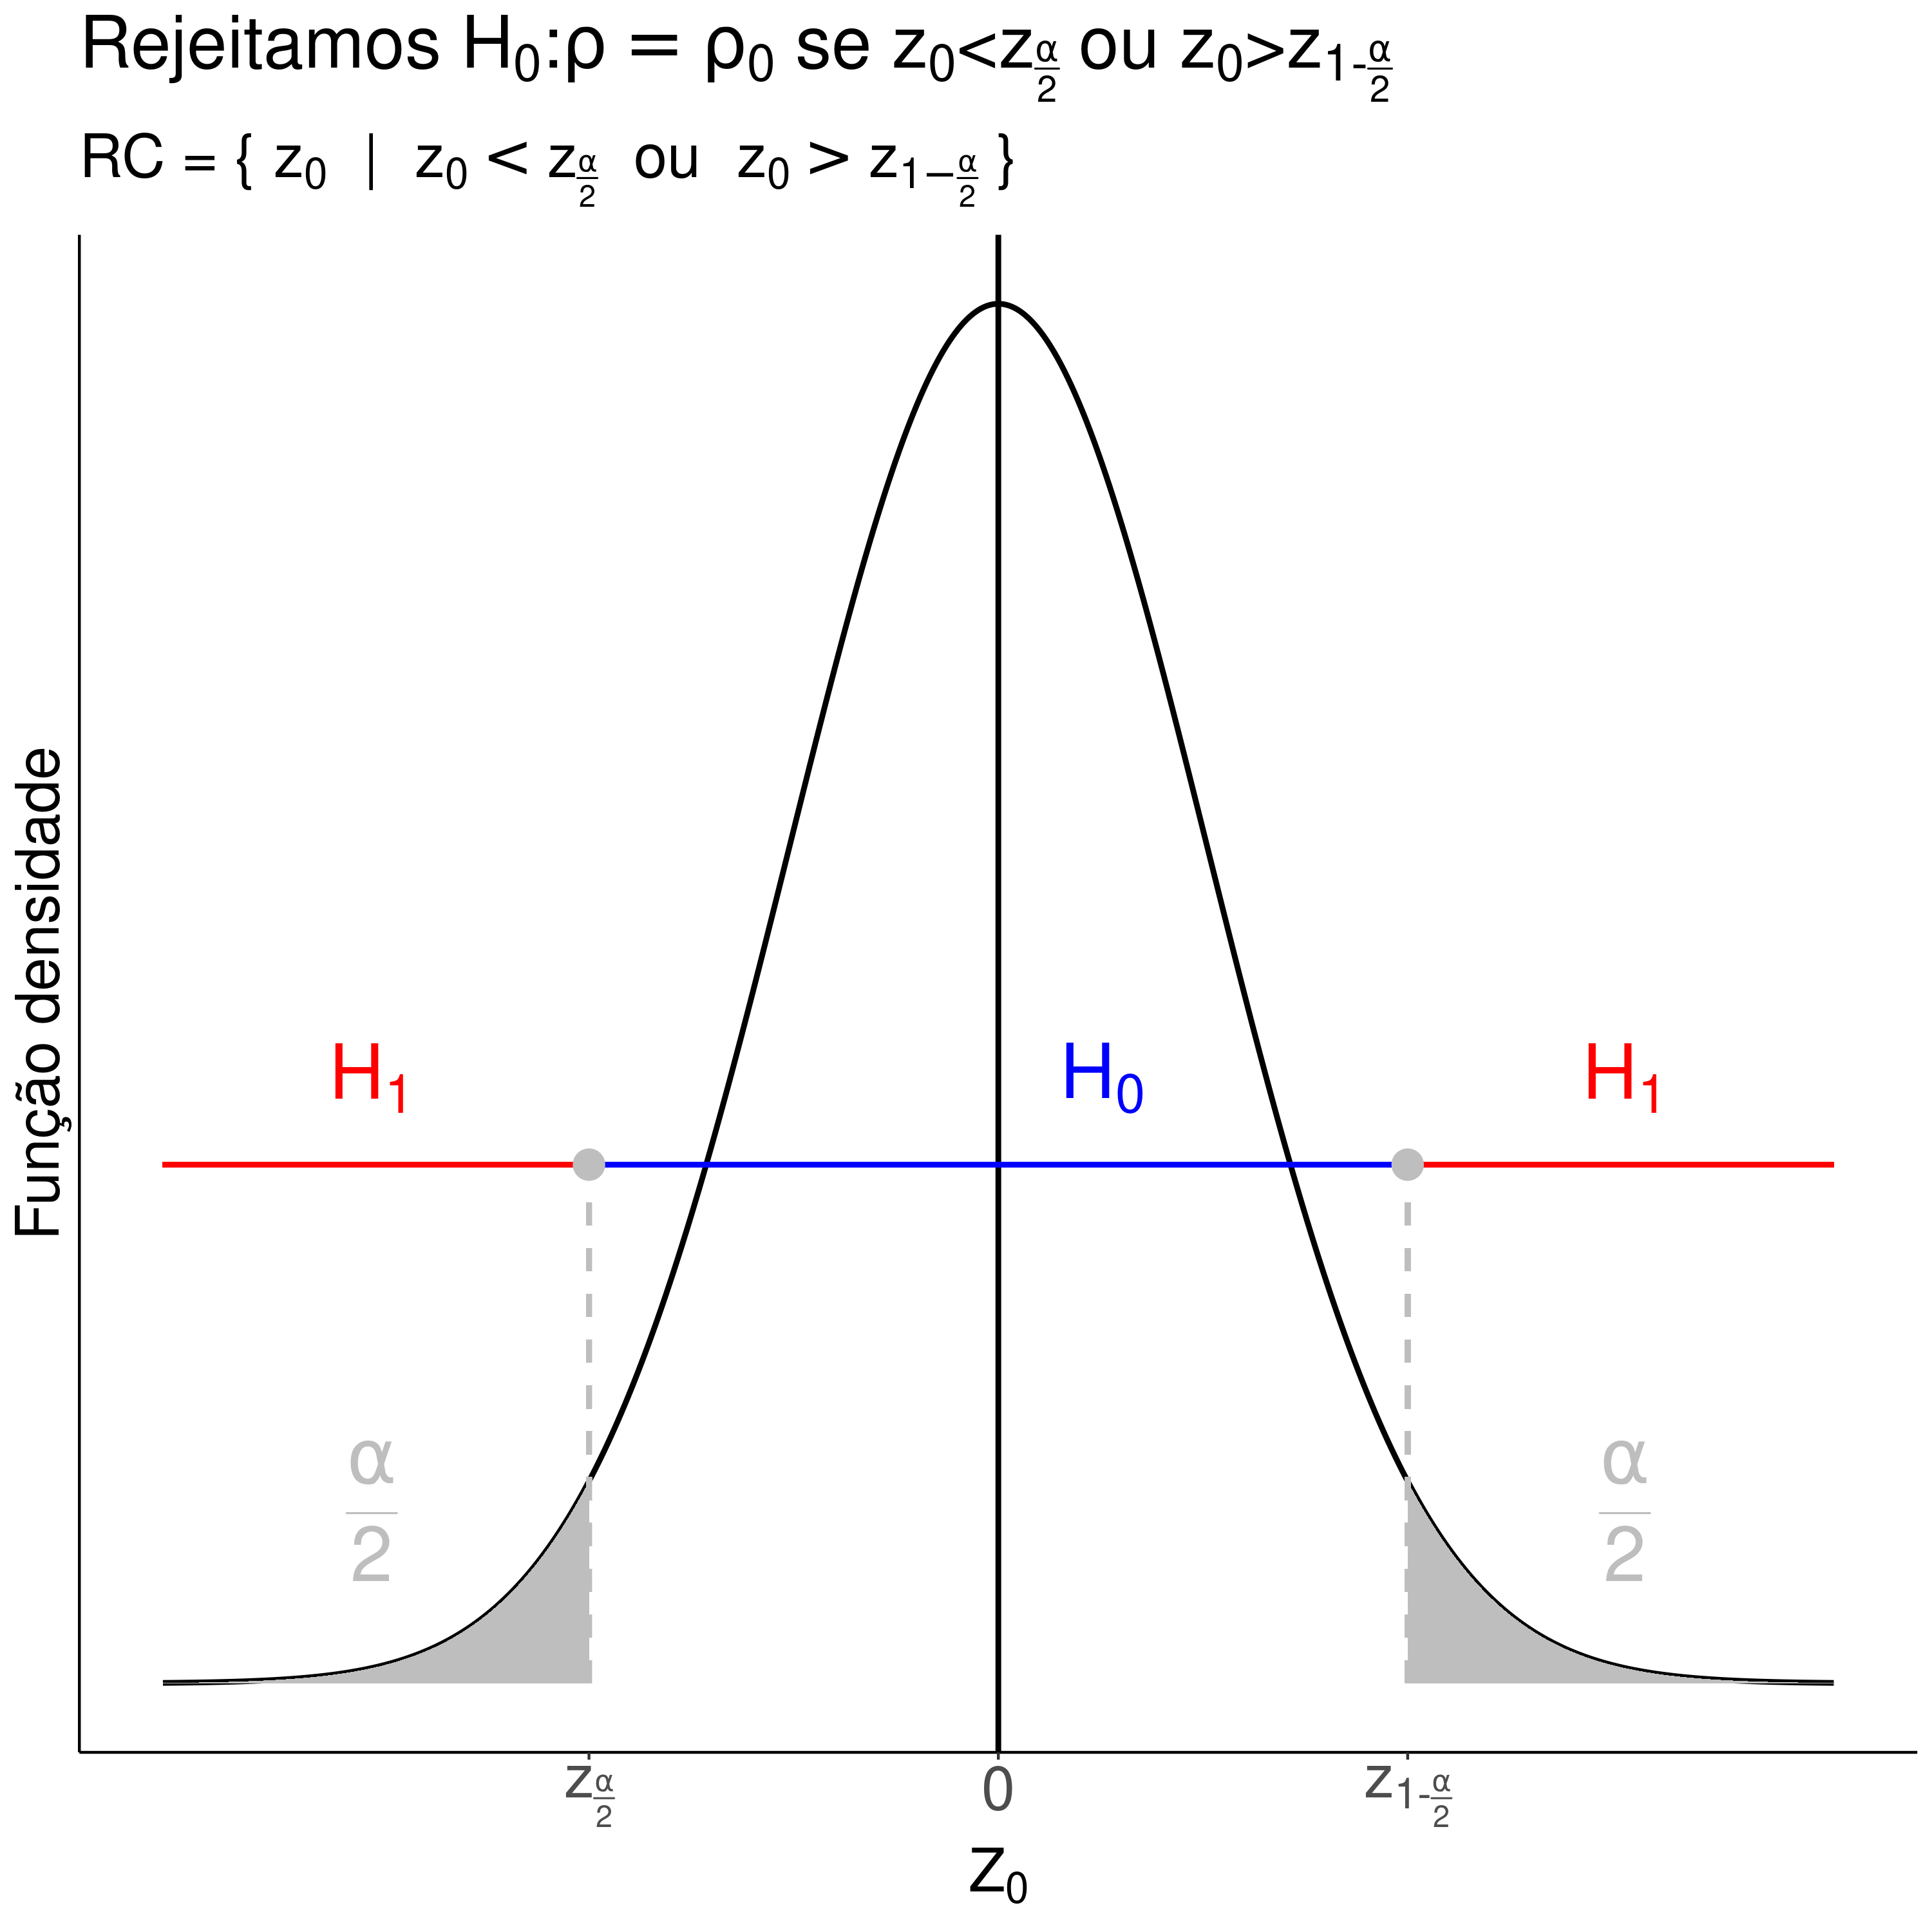
\includegraphics[width=0.32\linewidth]{figures/z-fisher-cor-bilateral.png} \label{fig:z-fisher-cor-bilateral}} \hfill
	\subfloat[][Teste bilateral.]{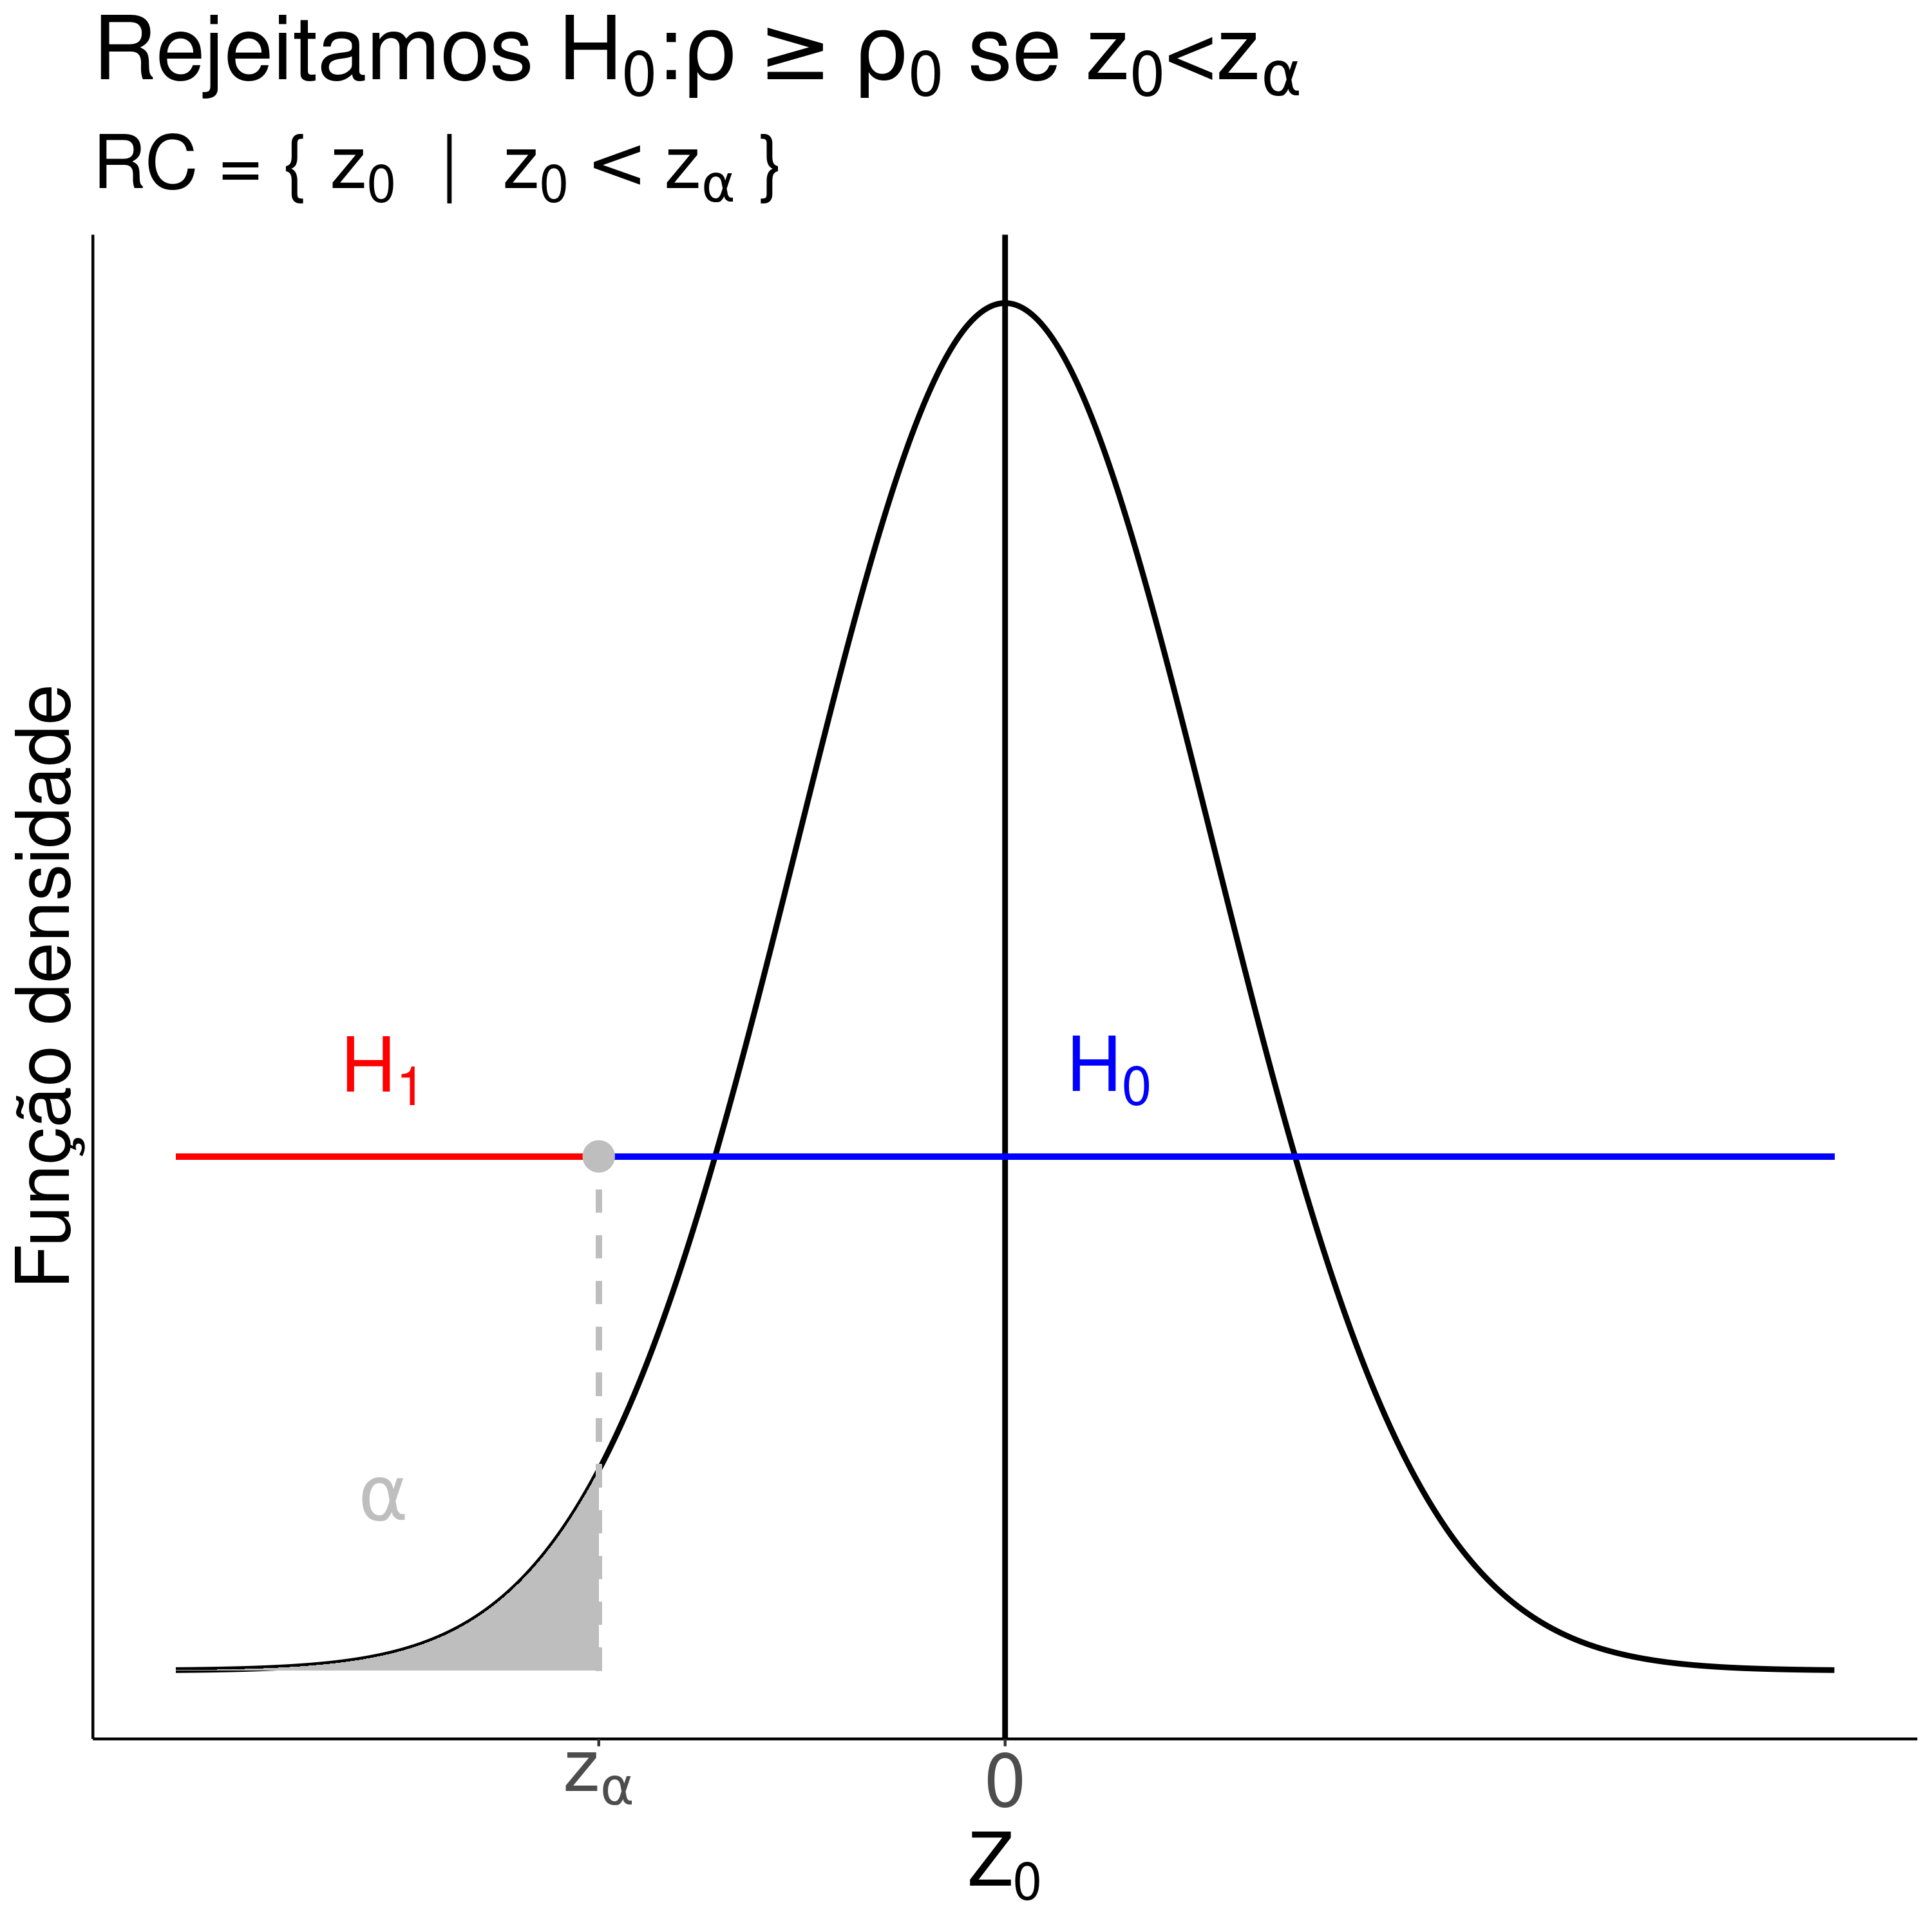
\includegraphics[width=0.32\linewidth]{figures/z-fisher-cor-h1-lower.png} \label{fig:z-fisher-cor-h1-lower}} \hfill
	\subfloat[][Teste bilateral.]{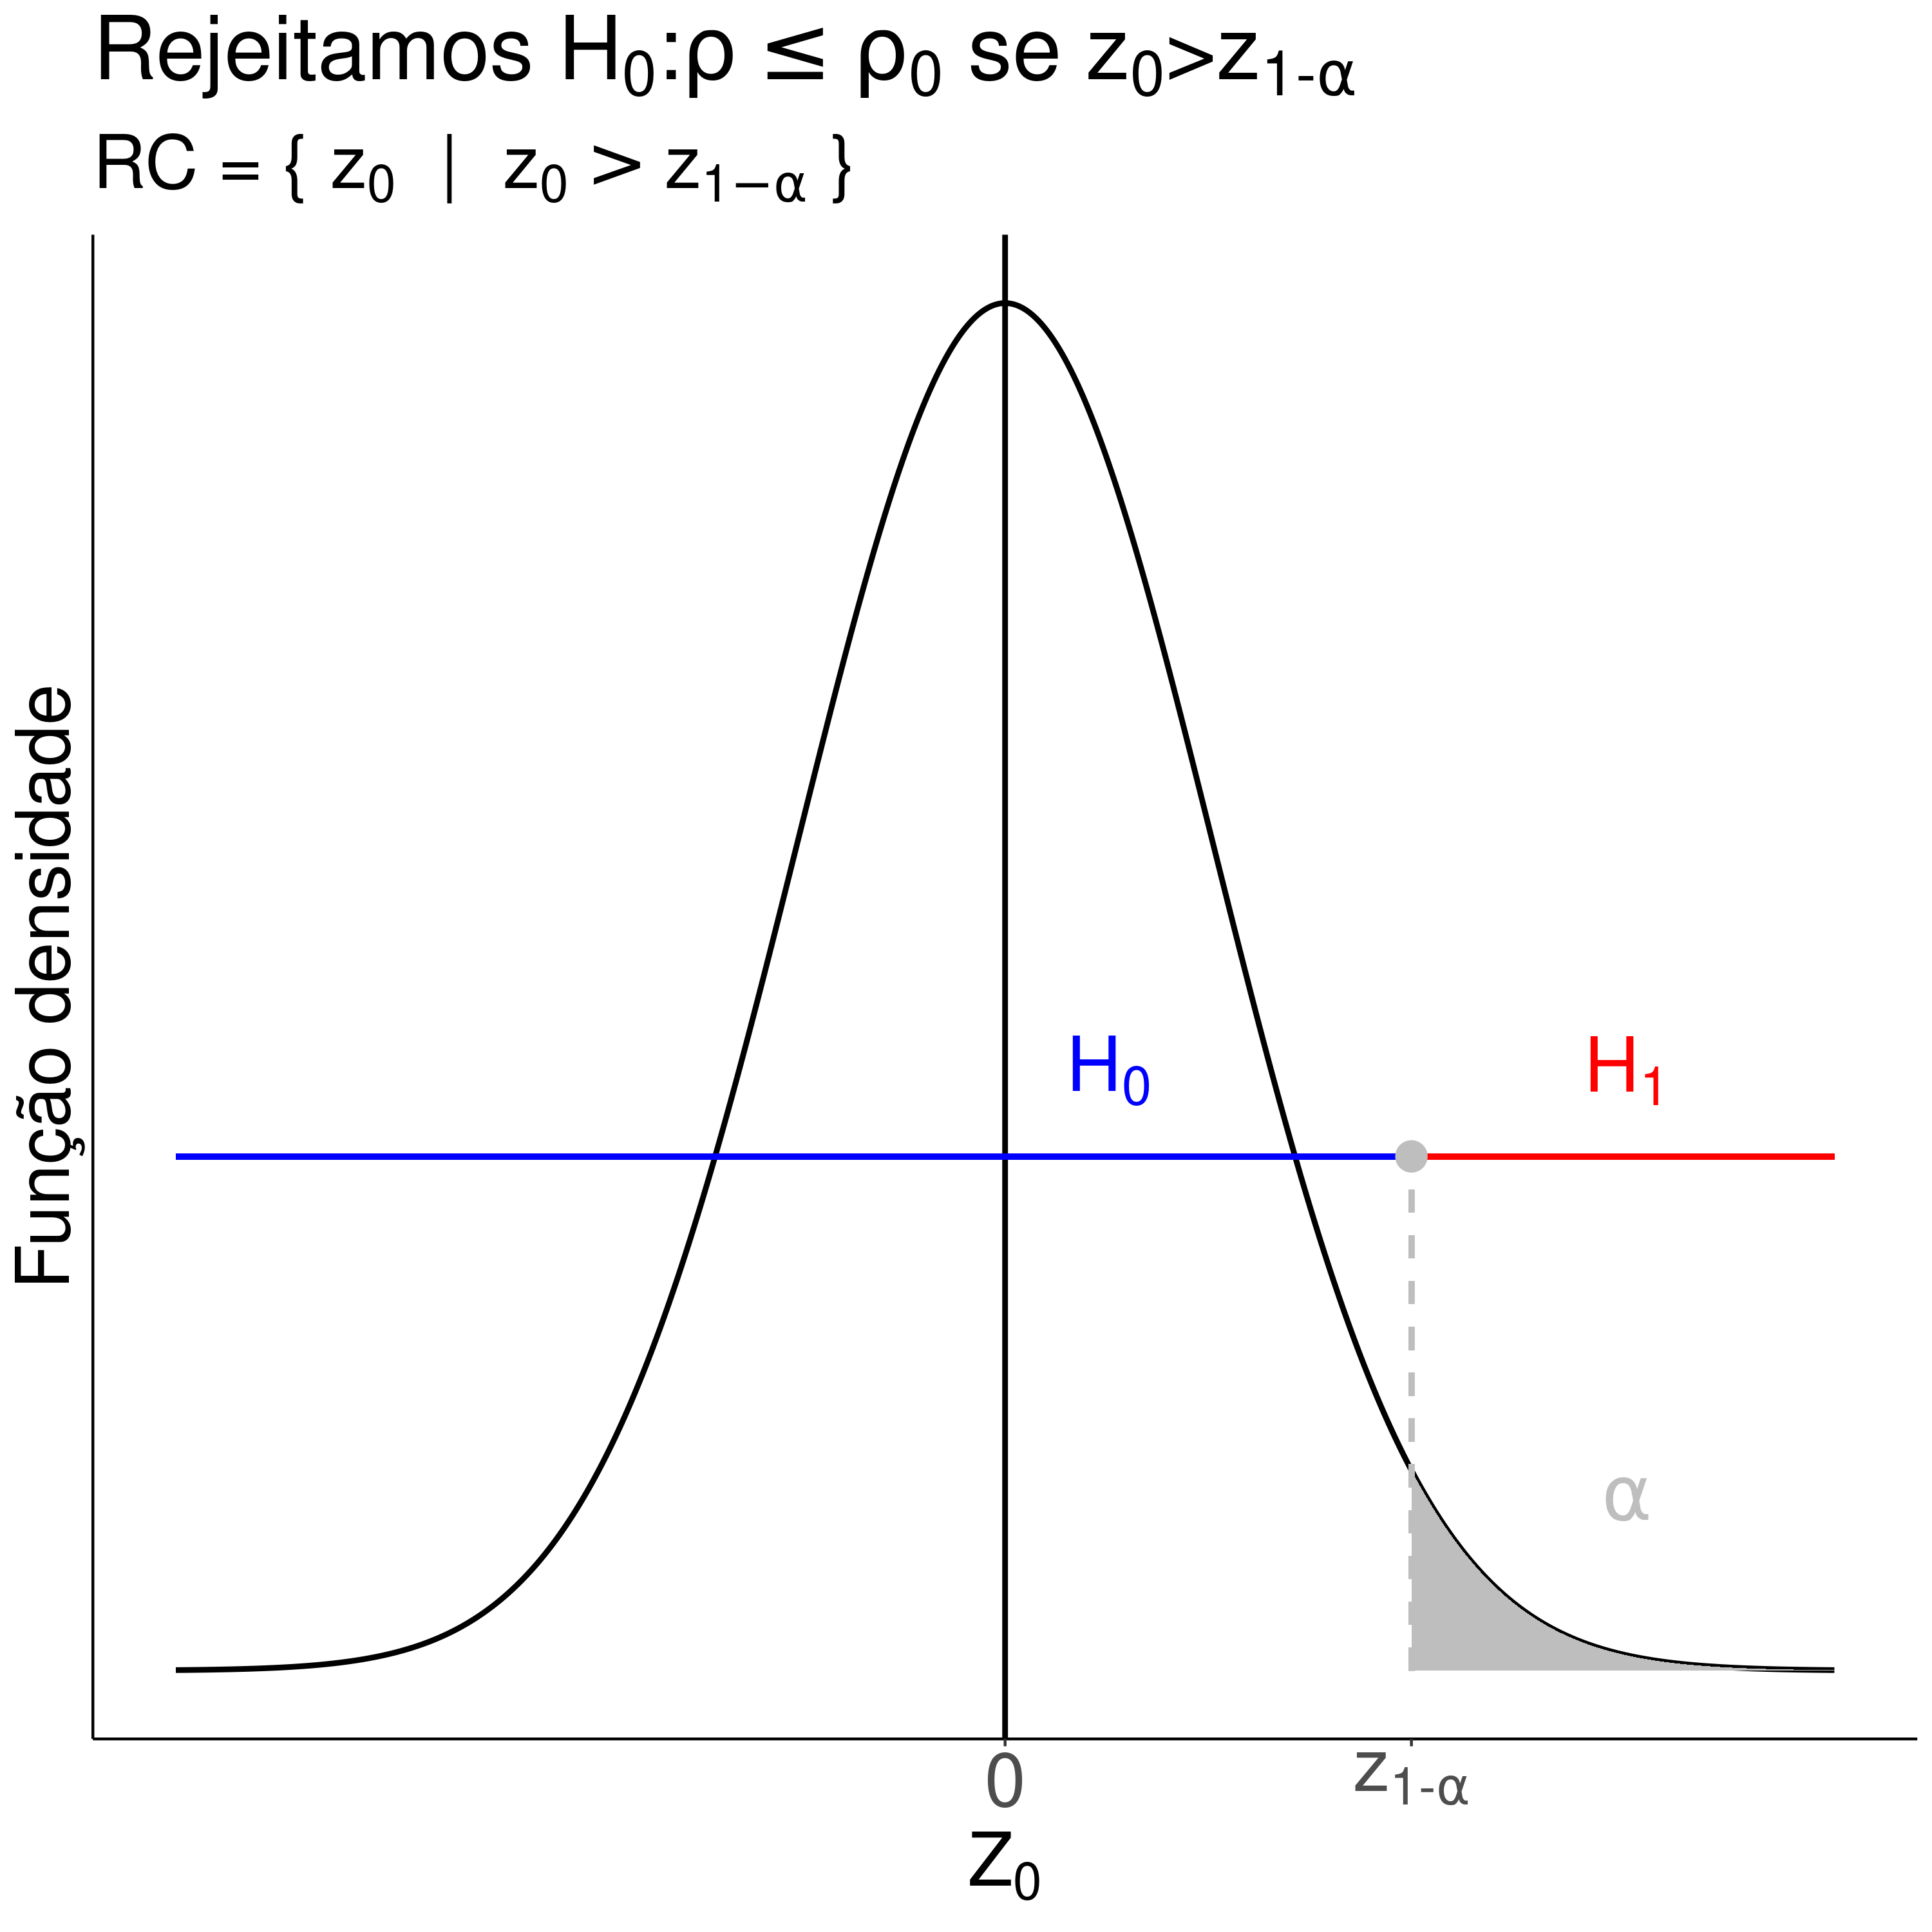
\includegraphics[width=0.32\linewidth]{figures/z-fisher-cor-h1-upper.png} \label{fig:z-fisher-cor-h1-upper}} 
	\caption{Região crítica para o teste de correlação linear de Pearson.}
\end{figure}
\end{frame}

\begin{frame}{Teste de hipóteses para $\rho$.}

\normalsize

\begin{itemize}
	\item Na Figura~\ref{fig:z-fisher-cor-bilateral}, testamos $H_0: \rho = \rho_0$ versus $H_1: \rho \neq \rho_0$. Rejeitamos $H_0$ se $z_0 = \frac{ \frac{1}{2} \ln \left( \frac{1 + r}{1 - r} \right) - \frac{1}{2} \ln \left( \frac{1 + \rho_0}{1 - \rho_0} \right) }{\sqrt{\nicefrac{1}{n-3}}} \in  RC=\{z_0 \mid z_0 < z_{\frac{\alpha}{2}} \allowbreak \mbox{ ou } z_0 > z_{1-\frac{\alpha}{2}} \}$, em que $\Phi\left(z_{\frac{\alpha}{2}} \right) = \frac{\alpha}{2}$ e $\Phi\left(z_{1-\frac{\alpha}{2}} \right) = 1 - \frac{\alpha}{2}$;
	\vfill
	
	\item Na Figura~\ref{fig:z-fisher-cor-h1-lower}, testamos $H_0: \rho \leq \rho_0 $ versus $H_1: \rho > \rho_0$. Rejeitamos $H_0$ se $z_0 = \frac{ \frac{1}{2} \ln \left( \frac{1 + r}{1 - r} \right) - \frac{1}{2} \ln \left( \frac{1 + \rho_0}{1 - \rho_0} \right) }{\sqrt{\nicefrac{1}{n-3}}} \in \allowbreak RC=\{z_0 \mid z_0 > z_{1-\alpha}  \}$, em que $\Phi\left(z_{1-\alpha} \right) =1- \alpha$;
	\vfill
	
	\item Na Figura~\ref{fig:z-fisher-cor-h1-upper}, testamos $H_0: \rho \geq \rho_0$ versus $H_1: \rho  < \rho_0$. Rejeitamos $H_0$ se $z_0 = \frac{ \frac{1}{2} \ln \left( \frac{1 + r}{1 - r} \right) - \frac{1}{2} \ln \left( \frac{1 + \rho_0}{1 - \rho_0} \right) }{\sqrt{\nicefrac{1}{n-3}}} \in \allowbreak RC=\{z_0 \mid z_0 < z_{\alpha}  \}$, em que $\Phi\left(z_{1-\alpha} \right) =1- \alpha$.
\end{itemize}
$z_{\alpha}$, $z_{1-\alpha}$, $z_{\frac{\alpha}{2}}$ e $z_{1-\frac{\alpha}{2}}$ são chamados de valores críticos. 

\normalsize

\end{frame}

\begin{frame}{Teste de hipóteses para $\rho$.}
\begin{block}{Exemplo}
	Está sendo estudado o efeito do teor de ferro na capacidade de vigas de concreto. Os dados da Tabela~\ref{tab:vigas-test} apresentam os resultados obtidas em uma amostra. As duas variáveis estão correlacionadas? Use $\alpha=5\%$. Calcule o valor-p.
	\begin{table}[ht]
		\centering
		\scalebox{0.9}{
			\begin{tabular}{l|cccccccccc}
				\toprule[0.05cm]
				X: ferro(\% peso) & 5,4 & 6,8 & 6,9 & 7,3 & 7,7 & 8,1 & 8,2 & 8,5 & 8,6 & 8,9 \\ \midrule[0.025cm]
				Y: Carga (ton. / m$^2$) & 2,1 & 2,2 & 2,9 & 2,9 & 3,0 & 3,1 & 3,1 & 3,1 & 3,4 & 3,5 \\ \bottomrule[0.05cm]
			\end{tabular}
		}
		\caption{Amostra com 10 vigas.} 
		\label{tab:vigas-test}
	\end{table}
	Note que $S_{x}= 76,4$, $S_{Y}=29,3$, $S_{x^2}=593,86$, $S_{y^2}=87,71$ e $S_{xy} = 227,85$.
\end{block}
\end{frame}

\begin{frame}{Teste de hipóteses para $\rho$.}

\begin{block}{Solução}
	\textbf{Passo 1)} Queremos testar as seguintes hipóteses: $H_0: \rho  = \rho_0=0$ e $H_0: \rho  \neq \rho_0=0$;
	
	\textbf{Passo 2)} Nível de significância $\alpha=5\%$;
	
	\textbf{Passo 3)} Rejeitamos $H_0$ se $\lvert Z_0 \rvert = \left\lvert \frac{ \frac{1}{2} \ln \left( \frac{1 + r}{1 - r} \right) - \frac{1}{2} \ln \left( \frac{1 + \rho_0}{1 - \rho_0} \right) }{\sqrt{\nicefrac{1}{n-3}}} \right\rvert$ for grande. Ou seja, $RC = \left\{ z_0 \mid z_0 < z_\frac{\alpha}{2} \mbox{ ou } z_{1-\frac{\alpha}{2}}  < z_0\right\}$;
	
	\textbf{Passo 4)} Vamos encontrar os valores críticos:
	\begin{itemize}
		\item $\Phi\left(z_\frac{\alpha}{2}\right) = \Phi\left(z_{0,025}\right) = \frac{\alpha}{2} = 0,025$, então $z_{0,025} = -1,96$;
		\item $\Phi\left(z_{1-\frac{\alpha}{2}}\right) = \Phi\left(z_{0,975}\right) =1- \frac{\alpha}{2} = 0,975$, então $z_{0,975} = 1,96$.
	\end{itemize}

	\textbf{Passo 5)} Como $r = 0,92$, $\rho_0=0$, $n = 10$ e $Z_0 = \frac{\frac{1}{2} \ln\left( \frac{1+r}{1-r} \right) - \frac{1}{2} \ln\left( \frac{1 + \rho_0}{1 - \rho_0} \right) }{\sqrt{\nicefrac{1}{n - 3}}} =\allowbreak \frac{\frac{1}{2} \ln\left( \frac{1 + 0,92}{1 - 0,92} \right) - \frac{1}{2} \ln\left( \frac{1 + 0}{1 - 0} \right) }{\sqrt{\nicefrac{1}{10 - 3}}} = 4,20 \in RC$, então rejeitamos $H_0$. 
	
	Ou seja, ao nível de significância $\alpha=5\%$, as duas variáveis estão associadas.
\end{block}

\end{frame}

\begin{frame}{Teste de hipóteses para $\rho$.}

\begin{block}{Solução (valor-p)}
	O valor-p é dado por
	$$p = P \left( \lvert Z_0 \rvert > \lvert z_0 \rvert \right) = 2 \cdot\left[ 1 - \Phi \left( \lvert z_0 \rvert \right) \right] .$$
\end{block}

Como $r = 0,92$, $\rho_0=0$, $n = 10$ e $Z_0 = \frac{\frac{1}{2} \ln\left( \frac{1+r}{1-r} \right) - \frac{1}{2} \ln\left( \frac{1 + \rho_0}{1 - \rho_0} \right) }{\sqrt{\nicefrac{1}{n - 3}}} =\allowbreak \frac{\frac{1}{2} \ln\left( \frac{1 + 0,92}{1 - 0,92} \right) - \frac{1}{2} \ln\left( \frac{1 + 0}{1 - 0} \right) }{\sqrt{\nicefrac{1}{10 - 3}}} = 4,20$, o valor-p é dado por
\begin{align*}
	p &= 2 \cdot \left[ 1 - \Phi\left( \lvert z_0 \rvert\right) \right]\\
	&= 2 \cdot \left[ 1 - \Phi(4,20) \right]\\
	&= 2 \cdot \left[1 - 1\right]\\
	&= 0.
\end{align*}

Como $p = 0 < \alpha = 0,05$, rejeitamos $H_0$. Ou seja, ao nível de significância $\alpha=5\%$, o teor de ferro está associada com a capacidade das vigas de concreto.

\end{frame}

\begin{frame}{Teste de hipóteses para $\rho$.}

\begin{block}{Exemplo}
	Considere uma amostra com 10 funcionários e suponha que coletamos duas variáveis:
	\begin{itemize}
		\item $X$: Anos de serviços;
		\item $Y$: Número de clientes.
	\end{itemize}
	Os dados estão mostrados na Tabela~\ref{tab:positiva-test}. O coeficiente de correlação linear de Pearson é maior que $0,5$? Use $\alpha=5\%$. Calcule o valor-p.
	\begin{table}[ht]
		\centering
		\scalebox{0.75}{
			\begin{tabular}{c|c|c}
				\toprule[0.05cm]
				Agente & Anos de serviço ($X$) & Número de clientes ($Y$)\\ 
				\midrule[0.05cm]
				A & 2 & 48 \\ 
				B & 3 & 50 \\ 
				C & 4 & 56 \\ 
				D & 5 & 52 \\ 
				E & 4 & 43 \\ 
				F & 6 & 60 \\ 
				G & 7 & 62 \\ 
				H & 8 & 58 \\ 
				I & 8 & 64 \\ 
				J & 10 & 72 \\ 
				\bottomrule[0.05cm]
			\end{tabular}
		}
		\caption{Amostra de 10 corretores de seguros.} 
		\label{tab:positiva-test}
	\end{table}
\end{block}

\end{frame}


\begin{frame}{Teste de hipóteses para $\rho$.}

\begin{block}{Solução}
	\textbf{Passo 1)} Queremos testar as seguintes hipóteses: $H_0: \rho \leq \rho_0= 0,5$ e $H_1: \rho > \rho_0= 0,5$;
	
	\textbf{Passo 2)} Nível de significância $\alpha=5\%$;
	
	\textbf{Passo 3)} Rejeitamos $H_0$ se $Z_0 =  \frac{\frac{1}{2} \ln\left( \frac{1+r}{1-r} \right) - \frac{1}{2} \ln\left( \frac{1 + \rho_0}{1 - \rho_0} \right) }{\sqrt{\nicefrac{1}{n - 3}}}$ for grande. Ou seja, $RC = \left\{ z_0 \mid z_0 > z_{1-\alpha} \right\}$;
	
	\textbf{Passo 4)} Vamos encontrar o valor crítico:
	\begin{itemize}
		\item $\Phi\left( z_{1-\alpha} \right) = \Phi\left( z_{0,95} \right) = 1-\alpha = 0,95$, então $z_{0,95} = 1,65$;
	\end{itemize}

	\textbf{Passo 5)} Como $r = 0,88$, $\rho_0 = 0,5$, $n = 10$ e $Z_0 =  \frac{\frac{1}{2} \ln\left( \frac{1+r}{1-r} \right) - \frac{1}{2} \ln\left( \frac{1 + \rho_0}{1 - \rho_0} \right) }{\sqrt{\nicefrac{1}{n - 3}}}\allowbreak \frac{\frac{1}{2} \ln\left( \frac{1 + 0,88}{1 - 0,88} \right) - \frac{1}{2} \ln\left( \frac{1 + 0,5}{1 - 0,5} \right) }{\sqrt{\nicefrac{1}{10 - 3}}} = 2, 19 \in RC$, então rejeitamos $H_0$.
	
	Ou seja, o nível de significância $\alpha=5\%$, a coeficiente de correlação linear de Pearson é maior que $0,5$.
\end{block}

\end{frame}

\begin{frame}{Teste de hipóteses para $\rho$.}

\begin{block}{Solução (valor-p)}
	O valor-p é dado por
	$$p = P(Z_0 > z_0 \mid H_0) = 1 - \Phi(z_0).$$
	
	 Como $r = 0,88$, $\rho_0 = 0,5$, $n = 10$ e $Z_0 =  \frac{\frac{1}{2} \ln\left( \frac{1+r}{1-r} \right) - \frac{1}{2} \ln\left( \frac{1 + \rho_0}{1 - \rho_0} \right) }{\sqrt{\nicefrac{1}{n - 3}}}\allowbreak \frac{\frac{1}{2} \ln\left( \frac{1 + 0,88}{1 - 0,88} \right) - \frac{1}{2} \ln\left( \frac{1 + 0,5}{1 - 0,5} \right) }{\sqrt{\nicefrac{1}{10 - 3}}} = 2, 19$, então o valor-p é dado por
	 \begin{align*}
		 p &= 1 - \Phi(z_0)\\
		 &= 1 - \Phi(2,19)\\
		 &= 1 - 0,9857\\
		 &= 0,0143.
	 \end{align*}
	 
	 Como $p = 0,0143 < \alpha = 0,05$, rejeitamos $H_0$. Ou seja, a correlação linear de Pearson é maior que $0,5$ ao nível de significância $\alpha=5\%$.
\end{block}

\end{frame}

\begin{frame}{Teste de hipóteses para $\rho$.}

\begin{block}{Exemplo}
	Imagine que um pesquisador deseja checar se duas variáveis aleatórias -- $X$ e $Y$ -- com distribuição normal tem associação forte e negativa. Algumas informações estão na Tabela~\ref{tab:experimento-test-rho}. Complete esta tabela. Ao nível de significância $\alpha=5\%$, as duas variáveis estão fortemente e negativamente associadas? Use $\alpha=5\%$. Calcule o valor-p.
	
	\begin{table}[ht]
		\centering
		\begin{tabular}{c|c|c|c|c}
			\toprule[0.05cm]
			$s_x$ & $s_y$ & $s_x^2$ & $s_y^2$ & $s_{xy}$\\
			\midrule
			-0,49 & 2004,01 & 942,57 & 4960,45 & -934,66  \\ \midrule[0.05cm]
			  $n$ & $\alpha$ & Decisão & valor-p & $Z_0$ \\ \midrule
			  1000 & 0,05 &  &  &  \\ \bottomrule[0.05cm]
		\end{tabular}
		\caption{Algumas informações do experimento} 
		\label{tab:experimento-test-rho}
	\end{table}
\end{block}

\end{frame}

\begin{frame}{Teste de hipóteses para $\rho$.}

\begin{block}{Solução}
	\textbf{Passo 1)} Queremos testar as hipóteses: $H_0: \rho \geq -0,8$ e $H_1: \rho < -0,8$;
	
	\textbf{Passo 2)} Nível de significância $\alpha=5\%$;
	
	\textbf{Passo 3)} Rejeitamos $H_0$ se $Z_0 =  \frac{\frac{1}{2} \ln\left( \frac{1+r}{1-r} \right) - \frac{1}{2} \ln\left( \frac{1 + \rho_0}{1 - \rho_0} \right) }{\sqrt{\nicefrac{1}{n - 3}}}$ for pequeno. Ou seja, $RC = \left\{ z_0 \mid z_0 < z_{\alpha}  \right\}$;
	
	\textbf{Passo 4)} Vamos encontrar o valor crítico:
	\begin{itemize}
		\item $\Phi\left(z_\alpha\right) = \Phi\left(z_{0,05}\right) = \alpha = 0,05$, então $z_{0,05} = -1,65$.
	\end{itemize}

	Como, $\bar{x} = -0,049$ $\bar{y} = 200,401$, $r = \frac{s_{xy} - n \cdot \bar{x}\bar{y}}{\sqrt{ (s_{x^2} - n \cdot \bar{x}^2) (s_{y^2} - n \cdot \bar{y}^2) }} =\allowbreak \frac{-934,66 - 10 \cdot (-0,049) \cdot (200,401) }{\sqrt{ (942,57 - 10 \cdot (-0,049)^2) (4960,45 - 10 \cdot (200,401)^2) }} = -0,9896$, $\rho_0 = -0,8$, $n = 10$ e $Z_0 =  \frac{\frac{1}{2} \ln\left( \frac{1+r}{1-r} \right) - \frac{1}{2} \ln\left( \frac{1 + \rho_0}{1 - \rho_0} \right) }{\sqrt{\nicefrac{1}{n - 3}}}=\allowbreak \frac{\frac{1}{2} \ln\left( \frac{1 - 0,9896}{1 + 0,9896} \right) - \frac{1}{2} \ln\left( \frac{1 - 0,8}{1 + 0,8} \right) }{\sqrt{\nicefrac{1}{10 - 3}}}= -4,04 \in RC$, então rejeitamos $H_0$.
	
	Ou seja, ao nível de significância $\alpha=5\%$, as duas variáveis estão fortemente e negativamente associadas.
\end{block}

\end{frame}

\begin{frame}{Teste de hipóteses para $\rho$.}

\begin{block}{Solução (valor-p)}
	O valor-p é dado por
	$$p = P\left( Z_0 < z_0 \mid H_0 \right) = \Phi(z_0).$$
	
	Como, $\bar{x} = -0,049$ $\bar{y} = 200,401$, $r = \frac{s_{xy} - n \cdot \bar{x}\bar{y}}{\sqrt{ (s_{x^2} - n \cdot \bar{x}^2) (s_{y^2} - n \cdot \bar{y}^2) }} =\allowbreak \frac{-934,66 - 10 \cdot (-0,049) \cdot (200,401) }{\sqrt{ (942,57 - 10 \cdot (-0,049)^2) (4960,45 - 10 \cdot (200,401)^2) }} = -0,9896$, $\rho_0 = -0,8$, $n = 10$ e $Z_0 =  \frac{\frac{1}{2} \ln\left( \frac{1+r}{1-r} \right) - \frac{1}{2} \ln\left( \frac{1 + \rho_0}{1 - \rho_0} \right) }{\sqrt{\nicefrac{1}{n - 3}}}=\allowbreak \frac{\frac{1}{2} \ln\left( \frac{1 - 0,9896}{1 + 0,9896} \right) - \frac{1}{2} \ln\left( \frac{1 - 0,8}{1 + 0,8} \right) }{\sqrt{\nicefrac{1}{10 - 3}}}= -4,04$, então o valor-p é dado por
	\begin{align*}
		p &= \Phi(z_0)\\
		&= \Phi(-4,04)\\
		&= 0.
	\end{align*}
	
	Como $p = 0 < \alpha=0,05$, então rejeitamos $H_0$. Ou seja, ao nível de significância $\alpha=0,05$, as duas variáveis estão fortemente e negativamente associadas.
\end{block}

\end{frame}

\subsection{Poder e tamanho da amostra.}

\begin{frame}{Poder do teste: $H_0:\rho = \rho_0$ e $H_1: \rho \neq \rho_0$.}

\normalsize

Imagine que
\begin{itemize}
	\item Hipóteses: $H_0:\rho = \rho_0$ e $H_1: \rho \neq \rho_0$;
	\item $H_1$ é verdade, então $\rho \neq \rho_0$;
	\item $Z_0 = \frac{\frac{1}{2} \ln\left( \frac{1 + r}{1 - r} \right) - \frac{1}{2} \ln\left( \frac{1 + \rho_0}{1 - \rho_0} \right)}{\sqrt{\frac{1}{n-3}}} \sim N\left( \mu; 1 \right)$, em que $\mu = \frac{ \frac{1}{2} \ln\left( \frac{1 + \rho}{1 - \rho} \right) -\frac{1}{2} \ln\left( \frac{1 + \rho_0}{1 - \rho_0} \right)  }{\sqrt{\nicefrac{1}{n-3}}}$;
	\item Ao nível de significância $\alpha$, temos $RC = \{ z_0 \mid z_0 < z_{\frac{\alpha}{2}} \mbox{ ou } z_{1-\frac{\alpha}{2}} < z_0  \}$.
\end{itemize}
\vfill	

Poder do teste é dado
\begin{align*}
\textcolor{important}{1-\beta} &=1 - \left[P\left( z_{\frac{\alpha}{2}} \leq Z_0 \leq z_{1-\frac{\alpha}{2}} \mid H_1 \right)\right] = 1 - \left[P\left( z_{\frac{\alpha}{2}} \leq Z_0 \leq z_{1-\frac{\alpha}{2}} \mid \rho \neq \rho_0 \right)\right]\\
&=\textcolor{important}{1 - \Phi\left( z_{1-\frac{\alpha}{2}} - \mu \right) + \Phi\left( z_{\frac{\alpha}{2}} - \mu \right).}
\end{align*}
A \textcolor{important}{Função Poder}, dado o tamanho da amostra $n$, é uma função das médias populacionais na hipótese alternativa  $\pi: (-1, 1) - \{\rho_0\} \longrightarrow [0,1]$ dada por
\begin{align*}
\pi(\rho) = 1 - \Phi\left( z_{1-\frac{\alpha}{2}} - \mu \right) + \Phi\left( z_{\frac{\alpha}{2}} - \mu \right), \rho \in (-1, 1) - \{\rho_0\}.
\end{align*}
Alguns livros chamam a Função Poder de \textcolor{important}{Curva de Característica Operacional.}

\normalsize

\end{frame}


\begin{frame}{Tamanho da amostra: $H_0:p_1 - p_2 = \Delta_0$ e $H_1: p_1 - p_2 \neq \Delta_0$.}

\normalsize
Imagine que
\begin{itemize}
	\item Hipóteses: $H_0:\rho = \rho_0$ e $H_1: \rho \neq \rho_0$;
	\item $H_1$ é verdade, então $\rho \neq \rho_0$;
	\item $Z_0 = \frac{\frac{1}{2} \ln\left( \frac{1 + r}{1 - r} \right) - \frac{1}{2} \ln\left( \frac{1 + \rho_0}{1 - \rho_0} \right)}{\sqrt{\frac{1}{n-3}}} \sim N\left( \mu; 1 \right)$, em que $\mu = \frac{ \frac{1}{2} \ln\left( \frac{1 + \rho}{1 - \rho} \right) -\frac{1}{2} \ln\left( \frac{1 + \rho_0}{1 - \rho_0} \right)  }{\sqrt{\nicefrac{1}{n-3}}}$;
	\item Ao nível de significância $\alpha$, temos $RC = \{ z_0 \mid z_0 < z_{\frac{\alpha}{2}} \mbox{ ou } z_{1-\frac{\alpha}{2}} < z_0  \}$.
\end{itemize}
\vfill

Considere $1-\beta$, $\alpha$, $\rho$ e $\rho_0$, então o tamanho \sout{mínimo} da amostra é solução da seguinte equação
\begin{align*}
1-\beta &= 1 - \Phi\left( z_{1-\frac{\alpha}{2}} - \mu \right) + \underbrace{\Phi\left( z_{\frac{\alpha}{2}} - \mu \right)}_{\approx 0} \approx 1 - \Phi\left( z_{1-\frac{\alpha}{2}} - \mu \right).
\end{align*}
Então, o tamanho \sout{mínimo} de amostra é dado por
$$n = \left\lceil \left[\frac{z_{1-\frac{\alpha}{2}} + z_{1-\beta} }{ \frac{1}{2} \ln \left( \frac{1 + \rho}{1 - \rho} \right) - \frac{1}{2} \ln \left( \frac{1 + \rho_0}{1 - \rho_0} \right) }\right]^2 + 3 \right\rceil $$
\normalsize

\end{frame}

\begin{frame}{Poder do teste: $H_0:\rho = \rho_0$ e $H_1: \rho \neq \rho_0$.}

\begin{block}{Exemplo}
	Está sendo estudado o efeito do teor de ferro na capacidade de vigas de concreto, ou seja, desejamos verificar se o teor de ferro está associado com a capacidade de vigas de concreto. Um pesquisador planeja estudar analisar $10$ vigas de concreto. E de outros estudos, o pesquisador acredita que $\rho = 0,95$. Qual o poder do teste? Use $\alpha=5\%$.

\end{block}

\end{frame}

\begin{frame}{Poder do teste: $H_0:\rho = \rho_0$ e $H_1: \rho \neq \rho_0$.}
\begin{block}{Solução}
	\textbf{Passo 1)} Queremos testar as hipóteses: $H_0: \rho = \rho_0$ e $H_1: \rho \neq \rho_0$;
	
	\textbf{Passo 2)} Nível de significância $\alpha=0,05$;
	
	Como $\rho = 0,95$, $\rho_0 = 0$, $n  =10$, $\mu = \frac{\frac{1}{2}\ln \left(\frac{1 + \rho}{1 - \rho}\right) - \frac{1}{2}\ln \left(\frac{1 + \rho_0}{1 - \rho_0}\right)}{\sqrt{\frac{1}{n-3}}} =\allowbreak \frac{\frac{1}{2}\ln \left(\frac{1 + 0,95}{1 - 0,95}\right) - \frac{1}{2}\ln \left(\frac{1 + 0}{1 - 0}\right)}{\sqrt{\frac{1}{10-3}}} = 4,85$. 
	
	Primeiro vamos encontrar os quantis:
	\begin{itemize}
		\item $\Phi\left( z_\frac{\alpha}{2} \right) = \Phi\left( z_{0,025} \right) = \frac{\alpha}{2} = 0,025$, então $z_{0,025} = -1,96$;
		\item $\Phi\left( z_{1-\frac{\alpha}{2}} \right) = \Phi\left( z_{0,975} \right) = 1-\frac{\alpha}{2} = 0,975$, então $z_{0,975} = 1,96$.
	\end{itemize}

	Então, o poder do teste é dado por
	\begin{align*}
		1-\beta &= 1 - \Phi\left( z_{1-\frac{\alpha}{2}} - \mu \right) + \Phi\left( z_{\frac{\alpha}{2}} - \mu \right) = 1 - \Phi\left(1,96 - 4,85\right) + \Phi\left( -1,96 - 4,85 \right)\\
		&= 1- \Phi\left( -2,89 \right) + \Phi\left( -6,81 \right) = 1  - 0,0019 + 0 = 0,9981.
	\end{align*}
\end{block}

\end{frame}

\begin{frame}{Tamanho do amostra: $H_0:\rho = \rho_0$ e $H_1: \rho \neq \rho_0$.}

\begin{block}{Exemplo}
	Está sendo estudado o efeito do teor de ferro na capacidade de vigas de concreto, ou seja, desejamos verificar se o teor de ferro está associado com a capacidade de vigas de concreto. E de outros estudos, o pesquisador acredita que $\rho = 0,95$. Dados o poder do teste $1-\beta = 0,99$, quantas vigas de concreto o pesquisador precisa analisar? Use $\alpha=5\%$.
	
\end{block}

\end{frame}

\begin{frame}{Tamanho do amostra: $H_0:\rho = \rho_0$ e $H_1: \rho \neq \rho_0$.}

\footnotesize
\begin{block}{Solução}
	\textbf{Passo 1)} Queremos testar as hipóteses: $H_0: \rho = \rho_0=0$ e $H_1: \rho \neq \rho_0 =0$;
	
	\textbf{Passo 2)} Nível de significância $\alpha=0,05$;
	
	Como $\rho = 0,95$, $\rho_0 = 0$, $n  =10$, $\mu = \frac{\frac{1}{2}\ln \left(\frac{1 + \rho}{1 - \rho}\right) - \frac{1}{2}\ln \left(\frac{1 + \rho_0}{1 - \rho_0}\right)}{\sqrt{\frac{1}{n-3}}} =\allowbreak \frac{\frac{1}{2}\ln \left(\frac{1 + 0,95}{1 - 0,95}\right) - \frac{1}{2}\ln \left(\frac{1 + 0}{1 - 0}\right)}{\sqrt{\frac{1}{10-3}}} = 4,85$. 
	
	Primeiro vamos encontrar os quantis:
	\begin{itemize}
		\item $\Phi\left( z_{1-\beta} \right) = \Phi\left( z_{0,99} \right) = 1-\beta = 0,99$, então $z_{0,99} = 2,33$;
		\item $\Phi\left( z_{1-\frac{\alpha}{2}} \right) = \Phi\left( z_{0,975} \right) = 1-\frac{\alpha}{2} = 0,975$, então $z_{0,975} = 1,96$.
	\end{itemize}
	
	Então, o tamanho \sout{mínimo} da amostra é dado por
	\begin{align*}
	n &= \left\lceil \left[ \frac{z_{1-\beta} + z_{1-\frac{\alpha}{2}}}{\frac{1}{2} \ln \left( \frac{1 + \rho}{1 - \rho} \right) - \frac{1}{2} \ln \left( \frac{1 + \rho_0}{1 - \rho_0} \right)} \right]^2  + 3\right\rceil = \left\lceil \left[ \frac{z_{0,99} + z_{0,975}}{\frac{1}{2} \ln \left( \frac{1 + 0,95}{1 - 0,95} \right) - \frac{1}{2} \ln \left( \frac{1 + 0}{1 - 0} \right)} \right]^2  + 3\right\rceil\\
	&= \left\lceil \left[ \frac{2,33 + 1,96}{\frac{1}{2} \ln \left( \frac{1 + 0,95}{1 - 0,95} \right) - \frac{1}{2} \ln \left( \frac{1 + 0}{1 - 0} \right)} \right]^2  + 3\right\rceil = \lceil 8,48 \rceil = 9.
	\end{align*}
	
	Ou seja, precisamos analisar $n=9$ vigas de concreto.
\end{block}
\normalsize

\end{frame}

\begin{frame}{Poder do teste: $H_0:\rho \leq \rho_0$ e $H_1: \rho > \rho_0$.}

\normalsize

Imagine que
\begin{itemize}
	\item Hipóteses: $H_0:\rho \leq \rho_0$ e $H_1: \rho > \rho_0$;
	\item $H_1$ é verdade, então $\rho > \rho_0$;
	\item $Z_0 = \frac{\frac{1}{2} \ln\left( \frac{1 + r}{1 - r} \right) - \frac{1}{2} \ln\left( \frac{1 + \rho_0}{1 - \rho_0} \right)}{\sqrt{\frac{1}{n-3}}} \sim N\left( \mu; 1 \right)$, em que $\mu = \frac{ \frac{1}{2} \ln\left( \frac{1 + \rho}{1 - \rho} \right) -\frac{1}{2} \ln\left( \frac{1 + \rho_0}{1 - \rho_0} \right)  }{\sqrt{\nicefrac{1}{n-3}}}$;
	\item Ao nível de significância $\alpha$, temos $RC = \{ z_0 \mid z_0 > z_{1 - \alpha}   \}$.
\end{itemize}
\vfill	

Poder do teste é dado
\begin{align*}
\textcolor{important}{1-\beta} &=1 - \left[P\left( Z_0 \leq z_{1-\alpha} \mid H_1 \right)\right] = 1 - \left[P\left(  Z_0 \leq z_{1-\alpha} \mid \rho \neq \rho_0 \right)\right]\\
&=\textcolor{important}{1 - \Phi\left( z_{1-\alpha} - \mu \right).}
\end{align*}
A \textcolor{important}{Função Poder}, dado o tamanho da amostra $n$, é uma função das médias populacionais na hipótese alternativa  $\pi: (\rho_0, 1) \longrightarrow [0,1]$ dada por
\begin{align*}
\pi(\rho) = 1 - \Phi\left( z_{1-\alpha} - \mu \right), \rho \in (\rho_0, 1).
\end{align*}
Alguns livros chamam a Função Poder de \textcolor{important}{Curva de Característica Operacional.}

\normalsize

\end{frame}


\begin{frame}{Tamanho da amostra: $H_0:p_1 - p_2 \leq \Delta_0$ e $H_1: p_1 - p_2 > \Delta_0$.}

\normalsize
Imagine que
\begin{itemize}
	\item Hipóteses: $H_0:\rho \leq \rho_0$ e $H_1: \rho > \rho_0$;
	\item $H_1$ é verdade, então $\rho > \rho_0$;
	\item $Z_0 = \frac{\frac{1}{2} \ln\left( \frac{1 + r}{1 - r} \right) - \frac{1}{2} \ln\left( \frac{1 + \rho_0}{1 - \rho_0} \right)}{\sqrt{\frac{1}{n-3}}} \sim N\left( \mu; 1 \right)$, em que $\mu = \frac{ \frac{1}{2} \ln\left( \frac{1 + \rho}{1 - \rho} \right) -\frac{1}{2} \ln\left( \frac{1 + \rho_0}{1 - \rho_0} \right)  }{\sqrt{\nicefrac{1}{n-3}}}$;
	\item Ao nível de significância $\alpha$, temos $RC = \{ z_0 \mid z_0 > z_{1 - \alpha}   \}$.
\end{itemize}
\vfill

Considere $1-\beta$, $\alpha$, $\rho$ e $\rho_0$, então o tamanho \sout{mínimo} da amostra é solução da seguinte equação
\begin{align*}
1-\beta &= 1 - \Phi\left( z_{1-\alpha} - \mu \right).
\end{align*}
Então, o tamanho \sout{mínimo} de amostra é dado por
$$n = \left\lceil \left[\frac{z_{1-\alpha} + z_{1-\beta} }{ \frac{1}{2} \ln \left( \frac{1 + \rho}{1 - \rho} \right) - \frac{1}{2} \ln \left( \frac{1 + \rho_0}{1 - \rho_0} \right) }\right]^2 + 3 \right\rceil. $$
\normalsize

 \end{frame}

\begin{frame}{Poder do teste: $H_0:\rho \leq \rho_0$ e $H_1: \rho > \rho_0$.}

\begin{block}{Exemplo}
	Um gestor deseja verificar se a associação entre as variáveis
	\begin{itemize}
		\item $X$: Anos de serviços;
		\item $Y$: Número de clientes.
	\end{itemize}
	é  positiva e maior que $0,5$. Esse gestor coletou informações de 10 trabalhadores. Suponha que a correlação linear de Pearson populacional é $\rho=0,85$. Qual o poder do teste? Use $\alpha=5\%$. 
\end{block}

\end{frame}

\begin{frame}{Poder do teste: $H_0:\rho \leq \rho_0$ e $H_1: \rho > \rho_0$.}

\begin{block}{Solução}
	\textbf{Passo 1)} Queremos testar as hipóteses: $H_0: \rho \leq \rho_0= 0,5$ e $H_1:\rho > \rho_0= 0,5$;
	
	\textbf{Passo 2)} Nível de significância $\alpha=5\%$;
	
	Note que $\rho_0 = 0,5$, $\rho = 0,85$, $n = 10$ e $\mu = \frac{ \frac{1}{2} \ln\left( \frac{1 + \rho}{1 - \rho} \right) -\frac{1}{2} \ln\left( \frac{1 + \rho_0}{1 - \rho_0} \right)  }{\sqrt{\nicefrac{1}{n-3}}} = \allowbreak \frac{ \frac{1}{2} \ln\left( \frac{1 + 0,85}{1 - 0,85} \right) -\frac{1}{2} \ln\left( \frac{1 + 0,5}{1 - 0,5} \right)  }{\sqrt{\nicefrac{1}{10-3}}} = 1,87$.
	
	Primeiro calculamos o quantil da distribuição normal
	\begin{itemize}
		\item $\Phi\left( z_{1-\alpha} \right) = \Phi\left( z_{1-\alpha} \right) = 1 - \alpha = 0,95$, então $z_{0,95} = 1,65$.
	\end{itemize}

	Então, o poder do teste é dado por
	\begin{align*}
		1-\beta &= 1 - \Phi \left( z_{1-\alpha} - \mu \right)\\
		&= 1 - \Phi \left(1,65 - 1,87 \right)\\
		&= 1 - \Phi\left( -0,22 \right)\\
		&= 1 - 0,4129 = 0,5871.
	\end{align*}
\end{block}
\end{frame}

\begin{frame}{Tamanho de amostra: $H_0:\rho \leq \rho_0$ e $H_1: \rho > \rho_0$.}

\begin{block}{Exemplo}
	Um gestor deseja verificar se a associação entre as variáveis
	\begin{itemize}
		\item $X$: Anos de serviços;
		\item $Y$: Número de clientes.
	\end{itemize}
	é  positiva e maior que $r=0,5$. Suponha que a correlação linear de Pearson populacional é $\rho=0,85$. Dado o poder do teste $1-\beta=99\%$, precisamos entrevistar quantos trabalhadores? Use $\alpha=5\%$. 
\end{block}

\end{frame}

\begin{frame}{Tamanho de amostra: $H_0:\rho \leq \rho_0$ e $H_1: \rho > \rho_0$.}

\small
\begin{block}{Solução}
	\textbf{Passo 1)} Queremos testar as hipóteses: $H_0: \rho \leq \rho_0= 0,5$ e $H_1:\rho > \rho_0= 0,5$;

	\textbf{Passo 2)} Nível de significância $\alpha=5\%$;
	
	Note que $\rho_0 = 0,5$, $\rho = 0,85$, $n = 10$ e $\mu = \frac{ \frac{1}{2} \ln\left( \frac{1 + \rho}{1 - \rho} \right) -\frac{1}{2} \ln\left( \frac{1 + \rho_0}{1 - \rho_0} \right)  }{\sqrt{\nicefrac{1}{n-3}}} = \allowbreak \frac{ \frac{1}{2} \ln\left( \frac{1 + 0,85}{1 - 0,85} \right) -\frac{1}{2} \ln\left( \frac{1 + 0,5}{1 - 0,5} \right)  }{\sqrt{\nicefrac{1}{10-3}}} = 1,87$.
	
	Primeiro calculamos os quantis da distribuição normal
	\begin{itemize}
		\item $\Phi\left( z_{1-\alpha} \right) = \Phi\left( z_{1-\alpha} \right) = 1 - \alpha = 0,95$, então $z_{0,95} = 1,65$;
		\item $\Phi\left( z_{1-\beta} \right) = \Phi\left( z_{1-\beta} \right) = 1 - \beta = 0,99$, então $z_{0,99} = 2,33$ 
	\end{itemize}
	
	Então, o tamanho \sout{mínimo} é dado por
	\begin{align*}
		n &= \left\lceil \left[ \frac{z_{1-\beta} + z_{1-\alpha}}{ \frac{1}{2} \ln \left( \frac{1 + \rho}{1 - \rho} \right) - \frac{1}{2} \ln \left( \frac{1 + \rho_0}{1 - \rho_0} \right) } \right]^2 + 3 \right\rceil = \left\lceil \left[ \frac{2,33 + 1,65}{\frac{1}{2} \ln \left( \frac{1 + 0,85}{1 - 0,85} \right) - \frac{1}{2} \ln \left( \frac{1 + 0,5}{1 - 0,5} \right)} \right]^2 + 3 \right\rceil\\
		&= \lceil 34,70 \rceil = 35
	\end{align*}	
	
	Então, precisamos entrevistar $35$ funcionários.
\end{block}
\normalsize
\end{frame}

\begin{frame}{Poder do teste: $H_0:\rho \geq \rho_0$ e $H_1: \rho < \rho_0$.}

\normalsize

Imagine que
\begin{itemize}
	\item Hipóteses: $H_0:\rho \geq \rho_0$ e $H_1: \rho < \rho_0$;
	\item $H_1$ é verdade, então $\rho < \rho_0$;
	\item $Z_0 = \frac{\frac{1}{2} \ln\left( \frac{1 + r}{1 - r} \right) - \frac{1}{2} \ln\left( \frac{1 + \rho_0}{1 - \rho_0} \right)}{\sqrt{\frac{1}{n-3}}} \sim N\left( \mu; 1 \right)$, em que $\mu = \frac{ \frac{1}{2} \ln\left( \frac{1 + \rho}{1 - \rho} \right) -\frac{1}{2} \ln\left( \frac{1 + \rho_0}{1 - \rho_0} \right)  }{\sqrt{\nicefrac{1}{n-3}}}$;
	\item Ao nível de significância $\alpha$, temos $RC = \{ z_0 \mid z_0 < z_{\alpha}   \}$.
\end{itemize}
\vfill	

Poder do teste é dado
\begin{align*}
\textcolor{important}{1-\beta} &=1 - \left[P\left( Z_0 \geq z_{\alpha} \mid H_1 \right)\right] = \left[P\left(  Z_0 \leq z_{\alpha} \mid \rho \neq \rho_0 \right)\right]=\textcolor{important}{\Phi\left( z_{\alpha} - \mu \right).}
\end{align*}
A \textcolor{important}{Função Poder}, dado o tamanho da amostra $n$, é uma função das médias populacionais na hipótese alternativa  $\pi: (-1, \rho) \longrightarrow [0,1]$ dada por
\begin{align*}
\pi(\rho) = \Phi\left( z_{\alpha} - \mu \right), \rho \in (-1, \rho).
\end{align*}
Alguns livros chamam a Função Poder de \textcolor{important}{Curva de Característica Operacional.}

\normalsize

\end{frame}


\begin{frame}{Tamanho da amostra: $H_0:p_1 - p_2 \leq \Delta_0$ e $H_1: p_1 - p_2 > \Delta_0$.}

\normalsize
Imagine que
\begin{itemize}
	\item Hipóteses: $H_0:\rho \geq \rho_0$ e $H_1: \rho < \rho_0$;
	\item $H_1$ é verdade, então $\rho < \rho_0$;
	\item $Z_0 = \frac{\frac{1}{2} \ln\left( \frac{1 + r}{1 - r} \right) - \frac{1}{2} \ln\left( \frac{1 + \rho_0}{1 - \rho_0} \right)}{\sqrt{\frac{1}{n-3}}} \sim N\left( \mu; 1 \right)$, em que $\mu = \frac{ \frac{1}{2} \ln\left( \frac{1 + \rho}{1 - \rho} \right) -\frac{1}{2} \ln\left( \frac{1 + \rho_0}{1 - \rho_0} \right)  }{\sqrt{\nicefrac{1}{n-3}}}$;
	\item Ao nível de significância $\alpha$, temos $RC = \{ z_0 \mid z_0 < z_{\alpha}   \}$.
\end{itemize}
\vfill

Considere $1-\beta$, $\alpha$, $\rho$ e $\rho_0$, então o tamanho \sout{mínimo} da amostra é solução da seguinte equação
\begin{align*}
1-\beta &= \Phi\left( z_{\alpha} - \mu \right).
\end{align*}
Então, o tamanho \sout{mínimo} de amostra é dado por
$$n = \left\lceil \left[\frac{z_{1-\alpha} + z_{1-\beta} }{ \frac{1}{2} \ln \left( \frac{1 + \rho}{1 - \rho} \right) - \frac{1}{2} \ln \left( \frac{1 + \rho_0}{1 - \rho_0} \right) }\right]^2 + 3 \right\rceil. $$
\normalsize

\end{frame}


\begin{frame}{Poder do teste: $H_0:\rho \geq \rho_0$ e $H_1: \rho < \rho_0$.}

\begin{block}{Exemplo}
	Imagine que um pesquisador deseja checar se duas variáveis -- $X$ e $Y$ --  com distribuição normal tem associação forte e negativa. Algumas informações estão na Tabela~\ref{tab:experimento-test-rho-power}. Complete esta tabela. Suponha que o coeficiente de correlação linear de Pearson populacional é $\rho=-0,95$. Qual o poder do teste? Use $\alpha=5\%$.
	
	\begin{table}[ht]
		\centering
		\begin{tabular}{c|c|c|c|c}
			\toprule[0.05cm]
			$1-\beta$ & $\rho$ & $\alpha$ & $n$ & $\rho_0$ \\
			\midrule
			 & $-0,95$ & $0,05$ & $200$  &   \\ \bottomrule[0.05cm]
		\end{tabular}
		\caption{Algumas informações do experimento} 
		\label{tab:experimento-test-rho-power}
	\end{table}
\end{block}


\end{frame}

\begin{frame}{Poder do teste: $H_0:\rho \geq \rho_0$ e $H_1: \rho < \rho_0$.}

\begin{block}{Solução}
	\textbf{Passo 1)} Queremos testar as hipóteses: $H_0: \rho \geq \rho_0 = -0,8$ e $H_1:  \rho < \rho_0 = -0,8$
	
	\textbf{Passo 2)} Nível de significância $\alpha = 0,05$;
	
	Note que $\rho_0=-0,8$, $\rho=-0,95$, $n=200$ e $\mu = \frac{\frac{1}{2} \ln \left( \frac{1 + \rho}{1 - \rho} \right) - \frac{1}{2} \ln \left( \frac{1 + \rho_0}{1 - \rho_0} \right)}{\sqrt{\frac{1}{n-3}}}= \allowbreak \frac{\frac{1}{2} \ln \left( \frac{1 - 0,95}{1 + 0,95} \right) - \frac{1}{2} \ln \left( \frac{1 -0,8}{1 + 0,8} \right)}{\sqrt{\frac{1}{200-3}}} = -10,29$.
	
	Primeiro encontramos os quantis da distribuição normal:
	\begin{itemize}
		\item $\Phi\left(z_{\alpha}\right) = \Phi\left(z_{0,05}\right) = \alpha = 0,05$, então $z_{0,05} = -1,65$.
	\end{itemize}

	Então, o poder do teste é dado por
	\begin{align*}
		1 - \beta &= \Phi\left( z_\alpha - \mu \right)\\
		&= \Phi\left( -1,65 - (-10,29) \right)\\
		&= \Phi(9,64)\\
		&= 1.
	\end{align*}
\end{block}

\end{frame}

\begin{frame}{Tamanho de amostra: $H_0:\rho \geq \rho_0$ e $H_1: \rho < \rho_0$.}

\begin{block}{Exemplo}
	Imagine que um pesquisador deseja checar se duas variáveis -- $X$ e $Y$ -- com distribuição normal tem associação forte e negativa. Algumas informações estão na Tabela~\ref{tab:experimento-test-rho-samp-size}. Complete esta tabela. Suponha que o coeficiente de correlação linear de Pearson populacional é $\rho=-0,95$. Para termos um poder de teste $99\%$, qual deve ser o tamanho da amostra? Use $\alpha=5\%$.
	
	\begin{table}[ht]
		\centering
		\begin{tabular}{c|c|c|c|c}
			\toprule[0.05cm]
			$1-\beta$ & $\rho$ & $\alpha$ & $n$ & $\rho_0$ \\
			\midrule
		 $99\%$	& $-0,95$ & $0,05$ &   &   \\ \bottomrule[0.05cm]
		\end{tabular}
		\caption{Algumas informações do experimento} 
		\label{tab:experimento-test-rho-samp-size}
	\end{table}
\end{block}

\end{frame}

\begin{frame}{Tamanho de amostra: $H_0:\rho \geq \rho_0$ e $H_1: \rho < \rho_0$.}

\begin{block}{Solução}
	\textbf{Passo 1)} Queremos testar as hipóteses: $H_0: \rho \geq \rho_0 = -0,8$ e $H_1:  \rho < \rho_0 = -0,8$
	
	\textbf{Passo 2)} Nível de significância $\alpha = 0,05$;
	
	Note que $\rho_0=-0,8$, $\rho=-0,95$, $1-\beta = 0,99$ e $\mu = \frac{\frac{1}{2} \ln \left( \frac{1 + \rho}{1 - \rho} \right) - \frac{1}{2} \ln \left( \frac{1 + \rho_0}{1 - \rho_0} \right)}{\sqrt{\frac{1}{n-3}}}= \allowbreak \frac{\frac{1}{2} \ln \left( \frac{1 - 0,95}{1 + 0,95} \right) - \frac{1}{2} \ln \left( \frac{1 -0,8}{1 + 0,8} \right)}{\sqrt{\frac{1}{200-3}}} = -1,94$.
	
	Primeiro encontramos os quantis da distribuição normal:
	\begin{itemize}
		\item $\Phi\left(z_{1-\alpha}\right) = \Phi\left(z_{0,95}\right) =1- \alpha = 0,95$, então $z_{0,95} = 1,65$;
		\item $\Phi\left(z_{1 - \beta}\right) = \Phi\left(z_{0,99}\right) =1- \beta = 0,99$, então $z_{0,99} = 2,33$.
	\end{itemize}
	
	Então, o tamanho \sout{mínimo} de amostra é dado por
	\begin{align*}
		n &= \left\lceil \left[ \frac{z_{1-\beta} + z_{1-\alpha}}{ \frac{1}{2} \ln \left( \frac{1 + \rho}{1 - \rho} \right) - \frac{1}{2} \ln \left( \frac{1 + \rho_0}{1 - \rho_0} \right) } \right]^2 + 3  \right\rceil = \left\lceil \left[ \frac{2,33 + 1,65}{ \frac{1}{2} \ln \left( \frac{1 - 0,95}{1 + 0,95} \right) - \frac{1}{2} \ln \left( \frac{1 - 0,8}{1 + 0,8} \right) } \right]^2 + 3  \right\rceil\\
		&= \lceil 32,47 \rceil = 33.
	\end{align*}
\end{block}

\end{frame}

\subsection{Intervalo de Confiança para $\rho$.}

\begin{frame}{Intervalo de confiança para $\rho$.}

\normalsize

Sejam
\begin{itemize}
	\item $x_{1,1}, \dots, x_{1,n_1}$ valores amostrados da população 1 $N(\mu_1, \sigma_1^2)$;
	\item $x_{2,1}, \dots, x_{2,n_2}$ valores amostrados da população 2 $N(\mu_2, \sigma_2^2)$;
	\item $\gamma=1-\alpha$ é o coeficiente de confiança. (Geralmente, $\gamma=95\%$).
\end{itemize}
\vfill

Note que $Z =  \frac{ \frac{1}{2} \ln \left( \frac{1 + r}{1 - r} \right) - \frac{1}{2} \ln \left( \frac{1 + \rho}{1 - \rho} \right) }{\sqrt{\nicefrac{1}{n-3}}}  \sim N(0,1)$, e 
$$P\left( z_{\frac{\alpha}{2}} \leq \frac{ \frac{1}{2} \ln \left( \frac{1 + r}{1 - r} \right) - \frac{1}{2} \ln \left( \frac{1 + \rho}{1 - \rho} \right) }{\sqrt{\nicefrac{1}{n-3}}} \leq z_{1-\frac{\alpha}{2}} \right) = 1 - \alpha.$$
\vfill

Então o intervalo de confiança para $\rho$ com coeficiente de confiança $\gamma=1-\alpha$ é dado por
$$IC(\rho; \gamma) = \left( \dfrac{ \exp\left[ 2 \left( z_{\frac{\alpha}{2}} \sqrt{\dfrac{1}{n - 3}} + \xi \right) \right] - 1}{ \exp\left[ 2 \left( z_{\frac{\alpha}{2}} \sqrt{\dfrac{1}{n - 3}} + \xi \right) \right] + 1 }; \dfrac{ \exp\left[ 2 \left( z_{1-\frac{\alpha}{2}} \sqrt{\dfrac{1}{n - 3}} + \xi \right) \right] - 1}{ \exp\left[ 2 \left( z_{1-\frac{\alpha}{2}} \sqrt{\dfrac{1}{n - 3}} + \xi \right) \right] + 1 }  \right).$$
em que $\xi = \frac{1}{2} \ln \left(  \frac{1+r}{1-r}\right)$.

\normalsize
\end{frame}

\begin{frame}{Intervalo de confiança para $\rho$.}

\begin{block}{Exemplo}
	Uma amostra aleatória com $n=25$ observações no tempo de falha do componente eletrônico e a temperatura no ambiente de aplicação em que os componentes foram usados.Obteve-se $r = 0,83$. Construa um intervalo de confiança para $\rho$ Use $\gamma = 95\%$.
\end{block}

\end{frame}

\begin{frame}{Intervalo de confiança para $\rho$.}

 \begin{block}{Solução}
 	Note que $r = 0,83$, $n=25$ e $\xi = \frac{1}{2} \ln\left( \frac{1+r}{1-r} \right) = 1,19$.
 	
 	Primeiro vamos encontrar os quantis da distribuição normal padrão:
 	\begin{itemize}
 		\item $\Phi\left(z_{\frac{\alpha}{2}}\right) = \Phi\left(z_{0,025}\right) = \frac{\alpha}{2} = 0,025$, então $z_{0,025} = -1,96$;
 		\item $\Phi\left(z_{1-\frac{\alpha}{2}}\right) = \Phi\left(z_{0,975}\right) = 1-\frac{\alpha}{2} = 0,975$, então $z_{0,975} = 1,96$.
 	\end{itemize}
 
 	Então, o intervalo de confiança é dado por
 	\tiny
 	\begin{align*}
 	IC(\rho; 95\%) &= \left( \dfrac{ \exp\left[ 2 \left( z_{\frac{\alpha}{2}} \sqrt{\dfrac{1}{n - 3}} + \xi \right) \right] - 1}{ \exp\left[ 2 \left( z_{\frac{\alpha}{2}} \sqrt{\dfrac{1}{n - 3}} + \xi \right) \right] + 1 }; \dfrac{ \exp\left[ 2 \left( z_{1-\frac{\alpha}{2}} \sqrt{\dfrac{1}{n - 3}} + \xi \right) \right] - 1}{ \exp\left[ 2 \left( z_{1-\frac{\alpha}{2}} \sqrt{\dfrac{1}{n - 3}} + \xi \right) \right] + 1 }  \right)\\
 	&= \left( \dfrac{ \exp\left[ 2 \left( -1,96 \sqrt{\dfrac{1}{25 - 3}} + 1,19 \right) \right] - 1}{ \exp\left[ 2 \left( -1,96 \sqrt{\dfrac{1}{25 - 3}} + 1,19 \right) \right] + 1 }; \dfrac{ \exp\left[ 2 \left( 1,96 \sqrt{\dfrac{1}{25 - 3}} + 1,19 \right) \right] - 1}{ \exp\left[ 2 \left( 1,96 \sqrt{\dfrac{1}{25 - 3}} + 1,19 \right) \right] + 1 }  \right)\\
 	& = \left(0,65; 0,92\right).
 	\end{align*}
 \end{block}
\normalsize

Então, o coeficiente de correlação linear de Pearson está entre $0,65$ e $0,92$ com coeficiente de confiança $\gamma=95\%$.
\end{frame}

\end{document}

